
\RequirePackage[l2tabu, orthodox]{nag}

\documentclass[letterpaper, 11 pt]{report}
%\documentclass[a5paper, 8 pt]{extreport}
%\usepackage[a5paper, top = 1.0 in, bottom = 0.9 in]{geometry}
%\usepackage[pass]{geometry}

%\usepackage[sc]{mathpazo}
%\linespread{1.05}

\usepackage{garamondx}
\usepackage[garamondx,cmbraces]{newtxmath}

\usepackage[T2A, T1]{fontenc}
\usepackage[utf8]{inputenc}
\usepackage{CJKutf8}
\usepackage{mathtools}
\usepackage{amsfonts}
\usepackage{amsmath}
\usepackage{amssymb}
\usepackage{braket}
\usepackage{ellipsis}
\usepackage{microtype}
\usepackage{graphicx}
\usepackage{placeins}
\usepackage{booktabs}
\usepackage{caption}
\usepackage{subcaption}
\usepackage[usenames,dvipsnames]{xcolor}
\usepackage{setspace}
\usepackage[sc]{titlesec}
\usepackage[doi = false, url = false, isbn = false,
            maxbibnames = 99, sorting = none, backend = bibtex,
            giveninits = true, style = numeric-comp]{biblatex}
\usepackage[colorlinks, breaklinks=true]{hyperref}
\usepackage[toc,page]{appendix}


\usepackage{showlabels}

\widowpenalty=10000
\clubpenalty=10000

%change link colours:
\hypersetup{ linktocpage, colorlinks=true, linkcolor=blue,
             citecolor=blue, filecolor=blue, urlcolor=blue }

%Bibliography stuff:
\addbibresource{diss.bib}

%Make titles a link:
\newbibmacro{string+doiurlisbn}[1]{%
   \iffieldundef{doi}{%
      \iffieldundef{url}{%
         \iffieldundef{isbn}{%
            \iffieldundef{issn}{%
               #1%
            }{%
               \href{http://books.google.com/books?vid=ISSN\thefield{issn}}{#1}%
            }%
         }{%
            \href{http://books.google.com/books?vid=ISBN\thefield{isbn}}{#1}%
         }%
      }{%
         \href{\thefield{url}}{#1}%
      }%
   }{%
      \href{http://dx.doi.org/\thefield{doi}}{#1}%
   }%
}

\DeclareFieldFormat{title}{\usebibmacro{string+doiurlisbn}{\mkbibemph{#1}}}
\DeclareFieldFormat[article,incollection]{title}%
   {\usebibmacro{string+doiurlisbn}{\mkbibquote{#1}}}


\title{Dissertation: early version}
\author{Matthew Baxter}
\date{\today}

\begin{document}

\pagenumbering{alph}

\begin{titlepage}

   \centering

   {\Huge Ion-Atom Collisions:}

   {\large a time-dependent density-functional-theory perspective}

   \vspace{2 cm}

   \textsc{matthew baxter}

   \vspace{2 cm}

   \textsc{a dissertation submitted to the faculty of graduate studies in partial fulfillment of the
           requirements for the degree of doctor of philosophy}

   \vspace{2 cm}

   \textsc{graduate programme in the department of physics and astronomy}

   \textsc{york university}

   \textsc{toronto ontario}

   Month Year

   \vspace{3.5 cm}

   \copyright Matthew Baxter, Year (\textsc{CC BY} 4.0).

   \thispagestyle{empty}

\end{titlepage}

\cleardoublepage
\phantomsection
\addcontentsline{toc}{chapter}{Abstract}

\begin{abstract}

   \thispagestyle{plain}
   \pagenumbering{roman}
   \setcounter{page}{2}

   \onehalfspacing

   Time-dependent density functional theory (\textsc{tdft}) is an alternate formulation of $N$-body
   quantum mechanics which allows one to describe a system via the single-particle density, $n$, rather
   than the full $N$-body wave function. While this reformulation is in theory exact in practice it
   necessitates at least two approximations. First, the exchange-correlation potential which encodes the
   two-particle interactions present in the time-dependent Schr\"{o}dinger equation into the language
   of the single-particle description is not precisely know. Even if one had perfect knowledge of this
   potential a further approximation would be required when attempting to extract the values of
   observables as the exact relation between the one-particle density and most observables of interest
   is also unknown.

   This dissertation investigates these issues using ion-atom collision systems as a test-bed. First,
   the observable problem is explored in antiproton-helium, proton-helium, and He\textsuperscript{2+}-He
   collision systems. Total cross sections for all charge transfer processes in these systems, the
   observables of choice in the present situation, are determined using a two centred extension of a
   correlation-integral model.

   Following this theoretical total cross section results for all ionization/capture processes in the
   He\textsuperscript{+}-He collision system are presented in the approximate impact energy range
   10-1000~keV/amu. Calculations were performed within the framework of time-dependent spin-density
   functional theory (a spin-dependent extension of \textsc{tddft}). These cross sections are used as a
   bench mark to test an accurate exchange-correlation potential generated via the Krieger-Li-Iafrate
   approximation applied within the exchange-only limit (correlation is ignored). The results of two
   models, one where electron translation factors in the orbitals used to calculate the potential are
   ignored and another where partial electron translation factors are included, are compared with
   available experimental data as well as a selection of previous theoretical calculations.

\end{abstract}

\singlespacing

\setcounter{page}{3}

\cleardoublepage
\phantomsection
\addcontentsline{toc}{chapter}{Contents}
\tableofcontents

\cleardoublepage
\phantomsection
\addcontentsline{toc}{chapter}{List of Tables}
\listoftables

\cleardoublepage
\phantomsection
\addcontentsline{toc}{chapter}{List of Figures}
\listoffigures

\newpage

\pagenumbering{arabic}

\onehalfspacing  %spacing here

\begin{chapter}{Introduction \label{chap:intro}}

   Atomic collision systems are of interest both on their own merits, and for there potential in
   applications. As a  particular the He\textsuperscript{+}-He collision system, a focus of a large
   portion of the present work, is applicable in such diverse areas as fusion reactors~\cite{fusion1,
   fusion2}, astrophysics~\cite{astro1, astro2}, and dark matter detection~\cite{dmdet}.

   From the point of view of theory, atomic collision systems are often explored as test-beds for
   few-electron quantum dynamics. A helium-like target, consisting of two electrons and a nucleus, and a
   bare projectile represent the archetypal few-electron collision system. The simplest example of such
   a system uses an antiproton, the negatively charged antiparticle of the proton, as the projectile.
   With a negative projectile the collision may be treated as an effective one-centred system which
   involves electron excitation and ionization.

   One might envision more complex systems by simply increasing the number of electrons on the target
   however, a more useful course is to replace the negatively charged projectile with one that is
   positively charged. With a positive projectile one must consider electron transfer in addition to
   ionization processes.

   Even more complex collision systems may be created by adding active electrons to the projectile. With
   this addition one must consider various combinations of ionization from both centres as well as
   transfers between target and projectile.

   This chain of accruing complexity essentially describes the path of this work in which a series of
   increasingly involved collision systems are investigated. This sequence begins with a negative
   projectile with an antiproton-helium system. Following this two systems, proton-helium
   (\textit{p}-He) and fully stripped helium ions on helium (He\textsuperscript{2+}-He), involving
   positively charged projectiles are investigated. Finally, singly charged helium ions incident on
   helium atoms (He\textsuperscript{+}-He), a system which contains one electron on the projectile and
   two on the target, was studied.

   Solving the Schr\"{o}dinger equation describing a system of more than two particles is
   computationally taxing, even for a small number of particles (three or more). Thus, the so called
   few-body problem, tests the limits of current computational power.

   In the standard treatment of many-body quantum mechanics there is a well-established process for
   calculating observables from the full many-body wave function describing the system. In
   time-dependent density functional theory~\cite{tddft, ullrich} (\textsc{tddft}) one does not
   necessarily know the full wave function, instead one works with the one-particle density. This
   method is, in principle, just as accurate as the standard wave function treatment while, at the
   same time being far more computationally efficient.

   One down side is that, unlike in standard quantum mechanics, observables are not readily calculable,
   as they are from the many-electron wave function. While the Runge-Gross theorem~\cite{rgt} guarantees
   that all observables are expressible as functionals of the one-particle density, exact expressions
   are only available in a limited number of cases~\cite{obs_exac}. In most situations one is then
   forced to work with approximate observable functionals.

   Additionally, when working within the context of \textsc{tddft} one typically determines the
   one-particle density via an auxiliary system of non-interacting particles. To obtain this a new
   potential, the Kohn-Sham potential (\textsc{ks}), which encodes the interacting system into the
   language of non-interacting particles, must be introduced. As with the observables, mentioned above,
   this potential is an unknown functional of the one-particle density and, as such, must also be
   approximated. These issues will be laid out in greater detail in Chap.~\ref{chap:dft} where the
   relevant \textsc{dft} background material is presented.

   This discussion is followed in Chap.~\ref{chap:p-he2p-he} where the antiproton-, proton-, and
   He\textsuperscript{+2}-He collision systems are investigated. The chapter focuses on exploring the
   observable problem through an application of a correlation integral model~\cite{wb} to the
   aforementioned collision systems. The second of the main problems of \textsc{dft} is explored in
   Chap.~\ref{chap:hephe} where a procedure for accurately approximating the Kohn-Sham potential is
   implemented and applied to the He\textsuperscript{+}-He collision system. Finally, A summary of the
   results and conclusions of this work are given in Chap.~\ref{chap:con}.

   Atomic units ($\hbar = m_e = e = 1$) are used throughout unless otherwise stated.

\end{chapter}

\begin{chapter}{Density Functional Theory \label{chap:dft}}

   This chapter concerns itself with a brief introduction to the world of density-functional theory,
   both ground-state~\cite{dft-engel} (\textsc{dft}) and time-dependent~\cite{tddft, ullrich, marques-1}
   (\textsc{tddft}). This discussion begins with an overview  of various existence theorems central to
   density functional theory (Sec.~\ref{sec:dft}). Next the Kohn-Sham equations are introduced in
   Sec.~\ref{sec:ks}. More practical matters are considered when two of the main problems of density
   functional theory, the observable problem (Sec.~\ref{sec:obs}) and the determination of the
   exchange-correlation potential (Sec.~\ref{sec:xcpot}) are introduced. The discussion of the
   xc-potential is focused on the optimized potential method (Sec.~\ref{sec:opm}) and the
   Krieger-Li-Iafrate approximation (Sec.~\ref{sec:kli}).

   \begin{section}{\textsc{dft} and \textsc{tddft} Existence Theorems \label{sec:dft}}

      In the standard treatment of non-relativistic many-body quantum mechanics a system is described by
      a wavefunction $\Psi$ which, depending upon the situation, is determined by either the
      time-dependent Schr\"{o}dinger equation (\textsc{tdse})
      %
      \begin{equation} \label{eq:tdse}
         \hat{H}(t) \Psi(t) = i \frac{\mathrm{d} \Psi(t)}{\mathrm{d} t},
      \end{equation}
      %
      or the stationary Schr\"{o}dinger equation (\textsc{sse})
      %
      \begin{equation} \label{eq:sse}
         \hat{H} \Psi = E \Psi.
      \end{equation}
      %
      If the system in question consists of $N$ electrons then $\Psi$ becomes a function of $N$ position
      variables $\mathbf{r}_i$ and spin variables $\sigma_i = \uparrow,$ $\downarrow$. The Hamiltonian,
      $\hat{H}$, may be decomposed into a kinetic energy term
      %
      \begin{equation} \label{eq:Top}
         \hat{T} = -\frac{1}{2} \sum\limits^{N}_{j=1} \Delta_j,
      \end{equation}
      %
      an electron-electron term
      %
      \begin{equation} \label{eq:Vee}
         \hat{V}_{ee} = \frac{1}{2} \sum\limits^{N}_{k \neq j}
                        \frac{1}{\left| \mathbf{r}_k - \mathbf{r}_j \right|},
      \end{equation}
      %
      and a, possibly, time-dependent external potential
      %
      \begin{equation} \label{eq:Vext}
         \hat{V}_\mathrm{ext} = \sum\limits^{n}_{j = 1} v_\mathrm{ext} (\mathbf{r}_j, \sigma_j, t).
      \end{equation}
      %
      The function $\hat{V}_\mathrm{ext}$ contains all of the one-body interactions, including the
      nuclear and any external potentials.

      Given the one-particle electronic density
      %
      \begin{equation} \label{eq:dendef1}
         n(\mathbf{r}, t) = N \sum\limits_{\sigma_1 \dots \sigma_N} \int \mathrm{d}^3 r_2 \dots
                              \mathrm{d}^3 r_N \left| \Psi(\mathbf{r}, \sigma_1, \mathbf{r}_2,
                              \sigma_2, \dots, \mathbf{r}_N, \sigma_N) \right|^2
      \end{equation}
      %
      the Hohenberg–Kohn theorem~\cite{hk-theorem} in the stationary case and the Runge-Gross
      theorem~\cite{rgt} in the time-dependent case establish a one-to-one mapping between the
      one-particle density $n$ and the external potential $\hat{V}_\mathrm{ext}$. The potential is
      then a unique functional of the one-particle density
      %
      \begin{equation} \label{eq:vext-func}
         \hat{V}_\mathrm{ext} = \hat{V}_\mathrm{ext} [n].
      \end{equation}
      %
      It should be noted that for time-dependent systems this mapping is unique only up to the addition
      of an arbitrary time-dependent function. As this serves only to introduce a phase into the
      associated wave function $\Psi[\hat{V}_\mathrm{ext}]$ it can be safely ignored in all future
      discussions. For more on this see the discussion following Eq.~\eqref{eq:obsfunc1}.

      In general, the time-dependent external potential will also be a functional of the initial state
      of the system $\Psi_0$. For a system consisting of a single electron no such initial-state
      dependence exists~\cite{initial1, initial1-erratum}, for two or more electrons the initial-state
      dependence is not necessarily unique~\cite{initial2, initial2-re, initial2-rere, initial3}.
      Fortunately, in most cases of interest initial-state dependence is not an issue. As an example
      any system initially in the ground state, as is the case in this work, may appeal to the
      Hohenberg-Kohn theorem to guarantee that any functionals depend uniquely on the initial state.

      We have formulated the density-potential mapping for an explicitly spin-dependent system, it
      then must be noted that the original existence theorems were not formulated in such general terms.
      Luckily, generalizations for both the stationary~\cite{spin-dep1, spin-dep2} and
      time-dependent~\cite{td-spindep} cases to spin-polarized systems exist.

   \end{section}

   \begin{section}{The Kohn-Sham Equations \label{sec:ks}}

      In practice the correspondence between the density and potential is used to map the interacting
      many-body \textsc{sse} or \textsc{tdse} onto an auxiliary non-interacting system. The
      density-potential mappings discussed in the previous section allow one to rewrite the interacting
      system in terms of an auxiliary system of non-interacting particles described by the functions
      $\varphi_{j\sigma}$ ($j = 1, \dots, N_\sigma$, $N = N_\uparrow + N_\downarrow$) with
      %
      \begin{equation} \label{eq:dendef2}
         n = \sum\limits_{\sigma} \sum\limits_{j = 1}^{N_\sigma}
                           \left| \varphi_{j\sigma} \right|^2,
      \end{equation}
      %
      where $n$ is the one-particle density of the fully interacting system. The orbitals $\varphi_i$
      are determined through the stationary or time-dependent Kohn-Sham equations~\cite{ks-eq,
      spin-dep1, spin-dep3, tdks} (\textsc{sks}, \textsc{tdks} respectively)
      %
      \begin{equation} \label{eq:sks}
         \left( -\frac{\Delta}{2} + v^\sigma_\mathrm{\textsc{ks}}[n_\uparrow,
         n_\downarrow](\mathbf{r}) \right)
          \varphi_{j\sigma}(\mathbf{r}) = \epsilon_{j \sigma} \varphi_{j \sigma}(\mathbf{r}),
      \end{equation}
      %
      \begin{equation} \label{eq:tdks}
         i \frac{\partial}{\partial t} \varphi_{j\sigma} =
            \left( -\frac{\Delta}{2} +
            v^\sigma_\mathrm{\textsc{ks}}[n_\uparrow, n_\downarrow](\mathbf{r},t)
            \right) \varphi_{j\sigma}(\mathbf{r},t),
      \end{equation}
      %
      where the $\epsilon_{j \sigma}$ appearing in Eq.~\eqref{eq:sks} are the Kohn-Sham eigenvalues and
      the quantities $n_\uparrow$, $n_\downarrow$ are the spin-up/down one-particle densities defined by
      %
      \begin{equation} \label{eq:spinden}
         n_\sigma = \sum\limits_{j=1}^{N_\sigma} \left| \varphi_{j\sigma} \right|^2,
      \end{equation}
      %
      such that
      %
      \begin{equation} \label{eq:denconstraint}
         n = n_\uparrow + n_\downarrow.
      \end{equation}

      The potential in Eqs.~\eqref{eq:sks} and~\eqref{eq:tdks} is known as the Kohn-Sham potential. This
      potential may be simplified by splitting it into a series of less complex objects
      %
      \begin{equation} \label{eq:vks}
         v^\sigma_\mathrm{\textsc{ks}}[n_\uparrow, n_\downarrow] = v_\mathrm{ext} + v_\mathrm{H}[n]
            + v^\sigma_\mathrm{xc}[n_\uparrow, n_\downarrow].
      \end{equation}
      %
      The first term in this expression is the external potential, which is the potential
      $\hat{V}_\mathrm{ext}$ of Eqs.~\eqref{eq:sse} and~\eqref{eq:tdse} on the single-particle level.
      The next term is the Hartree screening potential
      %
      \begin{equation} \label{eq:vh}
         v_\mathrm{H}(\mathbf{r},t) = \int \frac{n(\mathbf{r}^\prime, t)}
            {\left| \mathbf{r} - \mathbf{r}^\prime\right|} \, \mathrm{d}^3 r^\prime.
      \end{equation}
      %
      The last term is the exchange-correlation potential which encodes the complicated
      electron-electron interaction potential into the language of the non-interacting system. For
      convenience this is often further broken down into separate exchange and correlation potentials
      %
      \begin{equation} \label{eq:vxc}
         v^\sigma_\mathrm{xc} = v^\sigma_\mathrm{x} + v^\sigma_\mathrm{c}.
      \end{equation}

   \end{section}

   \begin{section}{Observables \label{sec:obs}}

      In the standard treatment of many-body quantum mechanics there is a well established process for
      calculating observables from the full many-body wave function describing the system. For any
      solution $\Psi$, unique up to a phase factor, of the \textsc{sse} or \textsc{tdse} and any
      observable $\hat{O}$ we immediately have the unique functional
      %
      \begin{equation} \label{eq:obsfunc1}
         O[\Psi] = \braket{\Psi| \hat{O} | \Psi},
      \end{equation}
      %
      so long as $\hat{O}$ contains no time-derivative terms.

      The density-potential mappings of Sec.~\ref{sec:dft} provide the relation
      %
      \begin{equation} \label{eq:denpot}
         n \mapsto \hat{V}_\mathrm{ext}[n] + c(t).
      \end{equation}
      %
      As the function $c$ only serves to introduce another phase factor we may use the uniqueness of
      solutions of the \textsc{sse}/\textsc{tdse} to define a map
      %
      \begin{equation} \label{eq:obsfunc2}
         n \mapsto \hat{V}_\mathrm{ext} \mapsto \Psi \mapsto O
      \end{equation}
      %
      or, $O = O[n]$.

      In principle all observables are functionals of the one-particle density. However, in practice the
      exact functional is only known in a handful of cases~\cite[p.~211-213]{obs_exac}. This discussion
      will be made far more explicit in Sec.~\ref{sec:obs} where the difficulties of extracting
      observables, total cross sections in this case, are described in detail.

   \end{section}

   \begin{section}{xc-potential \label{sec:xcpot}}

      Consider the energy functional for the interacting system
      %
      \begin{equation} \label{eq:efunc}
         E[n] = \braket{\Psi[n] | \hat{H} | \Psi[n] }= T[n] + E_{ee}[n] + E_\mathrm{ext}[n]
      \end{equation}
      %
      where the energies on the right hand side are the contributions from the constituent operators
      Eq.~\eqref{eq:Top}--\eqref{eq:Vext}. Similarly, we may define the energy functional for the
      non-interacting, \textsc{ks}, system as
      %
      \begin{equation} \label{eq:esfunc}
         E_s[n] =  T_s[n] + E_\mathrm{xc}[n] + E_\mathrm{H}[n] + E_\mathrm{ext}[n].
      \end{equation}
      %
      Making use of the fact that the energy is a unique functional of the density it follows that
      %
      \begin{equation} \label{eq:exc}
         E_\mathrm{xc} = T - T_s + E_{ee} - E_\mathrm{H}.
      \end{equation}
      %
      Finally making use of the fact that the ground-state one-particle density will minimize the energy
      it follows that
      %
      \begin{equation} \label{eq:vxc-der}
         \frac{\delta E_\mathrm{xc}[n]}{\delta n_\sigma(\mathbf{r})}
            = v^\sigma_\mathrm{xc}[n](\mathbf{r}).
      \end{equation}
      %
      The universality of the xc-functional~\cite{dft-engel} means that once an approximation to
      $E_\mathrm{xc}$ has been found we may apply the resulting potential to any system. Of course,
      some approximations will be better suited to certain situations.

      There are a few caveats to apply Eq.~\eqref{eq:vxc-der}. First, the functional is only defined
      for the set of ground-state $v$-representable densities, those densities which arise as
      ground-state solutions of the \textsc{sse} for some potential $v$. The second problem follows
      from the first. Due to the fact that not all densities are $v$-representable~\cite{not-vrep1,
      not-vrep2, not-vrep3}, one must establish that the set of functions for which the functional is
      defined is dense enough to ensure the existence of the functional derivative. For densities
      defined on a lattice~\cite{vrep-lat} as well as the general case~\cite{nonint1, nonint2,
      vrep-levy1, not-vrep1, vrep-lieb, vrep-rev} both the issue of $v$-representability and the
      existence of the functional derivatives of the energy functional have been addressed.

      In the case of \textsc{tddft} one can no longer rely upon minimizing the energy functional when
      seeking solutions. Instead one looks for stationary points of the quantum mechanical
      action~\cite{qmaction}
      %
      \begin{equation} \label{eq:qmact}
         A[n] = \int^{t_f}_{t_i} \mathrm{d}t
            \braket{\Psi[n] |i\frac{\partial}{\partial t} -\hat{H}(t) | \Psi[n]}.
      \end{equation}
      %
      In analogy to the ground state case the exchange correlation part of the action may be defined in
      terms of the difference between the actions for the interacting and non-interacting systems. We
      then find at a stationary point:
      %
      \begin{equation} \label{eq:tdvxc-der}
         \frac{\delta A_\mathrm{xc}[n]}{\delta n_\sigma(\mathbf{r},t)}
            = v^\sigma_\mathrm{xc}[n](\mathbf{r},t).
      \end{equation}

      In addition to similar issues of $v$-representability and functional differentiability the action
      Eq.~\eqref{eq:qmact} does not distinguish the direction of time and thus its naive use may lead
      to violations of causality~\cite{tddft-causality}. The existence of functional derivatives has
      been established in a similar style as in the stationary case~\cite{td-welldef}. The problem of
      which densities are $v$-representable has also been solved~\cite{td-vrep}. The causality problem
      may be solved in several ways including extending the time domain to the Keldysh
      contour~\cite{caus-sol1} and relaxing the boundary condition on one end point of the time
      interval~\cite{caus-sol2}.

      The simplest explicit density functional is the local density approximation~\cite{ks-eq}
      (\textsc{lda}). At its simplest the \textsc{lda} approximates the energy functional of a general
      system as that of the homogeneous electron gas (\textsc{heg})
      %
      \begin{equation} \label{eq:ldaE}
         E^\textsc{lda}[n] = \int \mathrm{d}^3 r \, n(\mathbf{r}) \epsilon_\textsc{heg}(n),
      \end{equation}
      %
      where $\epsilon_\textsc{heg}$ is the energy density of the \textsc{heg}, which is a function of
      the density of the gas. Exchange contributions to $\epsilon_\textsc{heg}$ have been determined
      analytically~\cite{heg}.

      Taking things further one is led to the hierarchy of increasingly complex
      generalized gradient approximations and hybrid functionals~\cite{gga+}. For time-dependent systems
      one may simply apply one of the many ground-state functionals to arrive at an adiabatic
      approximation in which the xc-potential depends only on the instantaneous density. Going beyond
      the adiabatic approximation is possible, however such functionals are much more complex. As an
      example the fully time-dependent version of the \textsc{lda}, the local deformation
      approximation~\cite{TDLDefA1, TDLDefA2} (\textsc{tdld}ef\textsc{a}) can be mentioned. A complete
      description of the time-time dependent xc-potential is a complicated task. Such a model would need
      to capture a wide range of phenomena. It has been shown that derivative
      discontinuities~\cite{derDis} and memory effects (see, for instance, the discussions
      in~\cite{tddft} and \cite{ullrich}) are important.

      \begin{subsection}{Optimized Potential Method \label{sec:opm}}

         An alternate approach to the explicit density functionals mentioned above is to employ an
         implicit density functional. For an implicit functional the xc-potential may be determined
         indirectly from the \textsc{ks}-orbitals, and their eigenvalues, through a procedure known as
         the optimized potential method~\cite{opm1, opm2} (\textsc{opm}) for which there are several
         derivations~\cite{opm1, opm2, opm3, opm4, opm5, opm-rev}.

         Without reproducing too many long equations one may use Eq.~\eqref{eq:vxc-der} and several
         applications of the chain rule for functional derivatives to arrive at ($c.c.$ denoting the
         complex conjugate of the preceding term)
         %
         \begin{equation} \label{eq:opm1}
            \begin{split}
               v^\sigma_\mathrm{xc}(\mathbf{r}) & = \int \mathrm{d}^3 r^\prime
                  \frac{\delta v^\sigma_\mathrm{\textsc{ks}}(\mathbf{r^\prime})}
                       {\delta n_\sigma(\mathbf{r}) } \\
                                    & \times \sum\limits_{j} \left\{ \int \mathrm{d}^3 r^{\prime\prime}
                \left[
               \frac{\delta E_\mathrm{xc}}{\delta \varphi_{j\sigma}(\mathbf{r^{\prime\prime}}) }
               \frac{\delta \varphi_{j\sigma}(\mathbf{r^{\prime\prime}}) }
                    {\delta v^\sigma_\mathrm{\textsc{ks}}(\mathbf{r^{\prime}}) }
               + c.c.
            \right]
               + \frac{\delta \epsilon_k}{\delta v^\sigma_\mathrm{\textsc{ks}}(\mathbf{r^{\prime}})}
              \frac{\partial E_\mathrm{xc}}{\partial \epsilon_k}
            \right\}
            \end{split}
         \end{equation}
         %
         from which the \textsc{opm} integral equation is then derived. A similar derivation for the
         time-dependent case leads to the time-dependent \textsc{opm} equation~\cite{tdopm}. In either
         situation an appropriate choice of $E_\mathrm{xc}$ or $A_\mathrm{xc}$ can include both exchange
         and correlation effects~\cite{opm5, tdopm}. With that said the \textsc{opm} is typically used
         to calculate exact exchange using the functional
         %
         \begin{equation} \label{eq:xfunc}
            \begin{split}
               A_\mathrm{x}[\varphi_{j\sigma}(\mathbf{r},t)]
                 = & \int \mathrm{d} t \, E_\mathrm{x}[\varphi_{j\sigma}(\mathbf{r},t)] \\
                = & -\frac{1}{2} \int \mathrm{d} t \, \sum\limits_\sigma \sum\limits_{j,k}
                    \int\mathrm{d}^3 r \mathrm{d}^3 r^\prime \\
                   & \times \frac{ \varphi^*_{j\sigma}(\mathbf{r}^\prime,t)
                           \varphi^*_{k\sigma}(\mathbf{r},t)
                           \varphi_{j\sigma}(\mathbf{r},t) \varphi_{k\sigma}(\mathbf{r}^\prime,t)}
                   {\left| \mathbf{r} -\mathbf{r}^\prime \right|}.
            \end{split}
         \end{equation}

         After some work the stationary version of the exchange-only \textsc{opm} will then follow from
         Eqs.~\eqref{eq:opm1} and \eqref{eq:xfunc}. The result may be expressed, adapting the notation
         of~\cite{klieq}, as
         %
         \begin{equation} \label{eq:opmEq}
            \sum\limits_j \int \mathrm{d}^3 r^\prime
            \left[ v^\sigma_\mathrm{x}(\mathbf{r}^\prime)
                 - \tilde{v}_{j \sigma} (\mathbf{r}^\prime) \right]
                 G_{j \sigma}(\mathbf{r}^\prime, \mathbf{r}) \varphi^*_{j \sigma} (\mathbf{r}^\prime)
                 \varphi_{j \sigma} (\mathbf{r}) + c.c. = 0,
         \end{equation}
         %
         where $G_{j \sigma}$ are the Green's functions
         %
         \begin{equation}
            G_{j \sigma}(\mathbf{r}, \mathbf{r}^\prime) = \sum\limits_{k \neq j}
            \frac{\varphi_{k \sigma} (\mathbf{r}) \varphi^*_{k \sigma} (\mathbf{r}^\prime)}
            {\epsilon_{k \sigma} - \epsilon_{j \sigma}}
         \end{equation}
         %
         and
         %
         \begin{equation} \label{eq:tildev}
            \tilde{v}_{j \sigma} (\mathbf{r}) =  - \sum\limits_k \int \mathrm{d}^3 r^\prime
               \frac{ \varphi^*_{j \sigma} (\mathbf{r}^\prime) \varphi^*_{k \sigma} (\mathbf{r}^\prime)
                      \varphi_{k \sigma} (\mathbf{r}) }
                      {\left| \mathbf{r} - \mathbf{r}^\prime \right| \varphi^*_{j \sigma} (\mathbf{r})}.
         \end{equation}

      \end{subsection}

      \begin{subsection}{The Krieger-Li-Iafrate Approximation \label{sec:kli}}

         Solving of the full \textsc{opm} integral equation can be quite difficult. To aid in this
         process the Krieger-Li-Iafrate approximation~\cite{kli1} (\textsc{kli}) may be used. One can
         think of \textsc{kli} as a closure approximation where the complicated interactions between
         orbitals are simplified by the introduction of an average energy difference
         $\Delta \epsilon_\sigma \approx \epsilon_{k \sigma} - \epsilon_{j \sigma}$ in the Green's
         functions. Returning to the exchange-only example introduced earlier this approximation causes
         Eq.~\eqref{eq:opmEq} to become
         %
         \begin{equation} \label{eq:kliEq}
            v_\mathrm{x}^\sigma(\mathrm{r}) =
               \frac{\sum\limits_{j} \varphi^*_{j \sigma} (\mathbf{r}) \varphi_{j \sigma} (\mathbf{r})
               \left[ \tilde{v}_{j \sigma}(\mathbf{r}) + \bar{v}_{j \sigma \mathrm{x}}
                                               - \bar{v}_{j \sigma} \right]}{n(\mathbf{r})},
         \end{equation}
         %
         where
         %
         \begin{equation}
            \bar{v}_{j \sigma} = \int \mathrm{d}^3 r \, \varphi^*_{j \sigma} (\mathbf{r})
               \varphi_{j \sigma} (\mathbf{r}) \tilde{v}_{j \sigma} (\mathbf{r})
         \end{equation}
         %
         and $\bar{v}_{j \sigma \mathrm{x}}$ is defined similarly.

         If one then multiplies both sides of Eq.~\eqref{eq:kliEq} by $\varphi^*_{l \sigma} (\mathbf{r})
         \varphi_{l \sigma} (\mathbf{r})$ and integrates over $\mathrm{d}^3 r$ one is left with a set of
         linear equations for $\bar{v}^\sigma_{l \sigma}$. This approximation turns the complex
         \textsc{opm} integral equation into a much simpler linear system of equations.

         It should be noted that while several variations of the \textsc{kli} exist~\cite{kli1, kli2,
         kli3} they differ by only a term proportional to $\partial E_\mathrm{xc} / \partial \epsilon_k$
         which, for functionals such as the exact exchange functional that do not depend on the
         \textsc{ks} eigenvalues does not contribute. As one might expect the \textsc{kli} approximation
         is also applicable in the time-dependent regime~\cite{tdkli1, tdkli2, tdkli3}.

         For a wide range of systems \textsc{kli} and the full \textsc{opm} produce very similar
         results~\cite{opm-rev}. The success of both \textsc{opm} and \textsc{kli} potentials is due in
         part to the fact that both capture the correct asymptotics of the exchange potential
         %
         \begin{equation}
            \lim\limits_{r \rightarrow \infty} v_\mathrm{x}^\sigma (\mathbf{r}) = -\frac{1}{r}.
         \end{equation}

         This is not to say that the \textsc{kli} is perfect, it is still an approximation. Both the
         exact and \textsc{opm} exchange-correlation potentials satisfy
         %
         \begin{equation} \label{eq:zft}
            \int \mathrm{d}^3 r \, n(\mathbf{r}, t) \nabla v^\sigma_\mathrm{xc}(\mathbf{r},t) = 0.
         \end{equation}
         %
         This relation is often referred to as the zero-force theorem, the name coming from the obvious
         interpretation that the force deriving from the exchange-correlation potential exerts no net
         force on the electron cloud. An unfortunate consequence of the \textsc{kli} approximation is
         that it can lead to violations of the zero-force theorem which, in turn, can lead to
         auto-excitation~\cite{kli-zero-force}. This is particularly pertinent in collision systems
         where spurious excitations may artificially enhance electron transfer processes.

      \end{subsection}

   \end{section}

\end{chapter}

\begin{chapter}{Bare Ion-Helium Collisions \label{chap:p-he2p-he}}

   Correlation enters \textsc{tddft} calculations in two distinct ways. First of these is dynamic
   correlation, those effects which emerge from a full time-dependent correlation potential. These are
   precisely the effects we ignore through the use of the frozen correlation model which is discussed
   along side a description of the collision systems of interest in Sec.~\ref{sec:p-he2p-he-sys}.

   The second source of correlation comes from the density functional
   used in the determination of observables. This so called functional correlation is the main focus of
   this chapter. The exploration of this topic begins in Sec.~\ref{sec:phe2p-obs} were several
   observable functional approximations are introduced. The results of application of these models to
   $p$-He, He\textsuperscript{2+}-He, as well as $\bar{p}$-He collisions are presented and discussed in
   Sec.~\ref{sec:phe2p-res}.

   The analysis presented in this chapter closely follows that of~\cite{p-he2p-he}. Additionally, while
   some results for $\bar{p}$-He collision system are presented here the bulk of the theoretical
   underpinnings of this work are not as this represents work undertaken during the completion of the
   author's Master's thesis~\cite{thesis}. The $\bar{p}$-He cross sections reproduced in this
   dissertation are an updated version of the previous results making use of the improved averaging
   scheme (Sec.~\ref{sec:phe2p-det}) developed when investigating the $p$-He and
   He\textsuperscript{2+}-He systems.

   \begin{section}{Collision System \label{sec:p-he2p-he-sys}}

      For the current systems of interest, $\bar{p}$-He, $p$-He, and He\textsuperscript{2+}-He
      collisions, the \textsc{tdks} [Eq.~\eqref{eq:tdks}] are greatly simplified. First, the initial
      state of the helium atom will be a spin-singlet. As a result of this we need only consider one
      \textsc{ks}-orbital
      %
      \begin{equation} \label{eq:oneorb}
         \varphi = \varphi_{1\uparrow} = \varphi_{1\downarrow}.
      \end{equation}
      %
      With this in mind all spin indices will be suppressed for the remainder of this chapter. An
      additional consequence of the spin-singlet nature of the system is that the exchange potential
      takes the form
      %
      \begin{equation} \label{eq:vxvh}
         v_\mathrm{x} = - \tfrac{1}{2} v_\mathrm{H}.
      \end{equation}

      As in~\cite{pbarhe} the correlation potential $v_\mathrm{c}$ will be approximated using a frozen
      correlation model. This potential is determined by inverting the Kohn-Sham scheme for the density
      of an accurate multi-configuration Hartree-Fock~\cite{mchf} (\textsc{mchf}) ground-state helium
      wave function. The details of this process can be found in~\cite{thesis, pbarhe}.

      Finally, the external potential can be specified. For a collision system in the semi-classical
      approximation this consists of the Coulomb potentials of the nuclear centres of the target and
      projectile. We may write
      %
      \begin{equation} \label{eq:phe2p-ext}
         v_\mathrm{ext}(\mathbf{r},t) = -\frac{Q_T}{r}
         - \frac{Q_P}{\left| \mathbf{r} - \mathbf{R}(t) \right|},
      \end{equation}
      %
      where $Q_T$ and $Q_P$ are the charges of the target and projectile nuclei and
      $\mathbf{R}(t) = (b,0,V t)$ is the straight-line trajectory of the projectile with velocity $V$ and
      impact parameter (distance of closest approach) $b$. In the current work we consider antiprotons,
      protons, and He\textsuperscript{2+} ions incident on helium atoms, thus $Q_T = 2$ and
      $Q_P = -1$, 1, and 2 respectively.

      The \textsc{tdks} described above was solved with the basis generator method~\cite{bgm}
      (\textsc{bgm}) using a basis similar to the one employed in~\cite{keim-ihe}. As in~\cite{pbarhe}
      the basis rooted in an x-only description of the helium atom in~\cite{keim-ihe} is replaced by one
      that reflects the incorporation of the ground-state correlation potential. In the \textsc{bgm} we
      expand the time-dependent orbital in terms of the basis functions
      %
      \begin{equation} \label{eq:bgmbasis}
         \chi^{KJ}_k (\mathbf{r},t)
         = W_T(r,\epsilon_T)^K W_P( \mathbf{r},t, \epsilon_P)^J \chi^{00}_k (\mathbf{r}),
      \end{equation}
      %
      with
      %
      \begin{equation}
         W_T(r,\epsilon_T) = \frac{1 - e^{-\epsilon_T r}}{r},
      \end{equation}
      %
      \begin{equation}
         W_P (\mathbf{r},t,\epsilon_P)
         = \frac{1 - e^{-\epsilon_P|\mathbf{r} - \mathbf{R}(t)|}}{|\mathbf{r} - \mathbf{R}(t)|}
      \end{equation}
      %
      and $\chi^{00}_k$ the eigenstates of the initial Hamiltonian (in this case the ground-state
      Kohn-Sham system for the helium atom). In order to keep the number of states in the basis to a
      minimum and simplify the description only those states with $K = 0$ where included. This
      simplification has proved sufficient in the past~\cite{bgm-rev}. The remaining regularizer is set
      to $\epsilon_P = 1$. A more general two-centred version of the \textsc{bgm} (\textsc{tc-bgm})
      which includes explicit basis states on both the target and the potential is also possible. The
      full machinery of the two-centred will be discussed in the following chapter.

   \end{section}

   \begin{section}{Approximating Observable Functionals \label{sec:phe2p-obs}}

      The discussion started in Sec.~\ref{sec:obs} may be elaborated upon by introducing the observables
      of interest for our ion-atom collision systems, the ionization and capture probabilities. For both
      negatively and positively charged projectiles we must consider the two pure ionization processes,
      single ionization
      %
      \begin{equation} \label{eq:TI}
         A^z + \mathrm{He} \rightarrow A^z + \mathrm{He}^+ + e^-
      \end{equation}
      %
      and double ionization
      %
      \begin{equation} \label{eq:II}
         A^z + \mathrm{He} \rightarrow A^z + \mathrm{He}^{2+} + 2e^-,
      \end{equation}
      %
      where $A^z = \mathrm{H}^+$ or $p$ for protons, $A^z = \mathrm{He}^{2+}$, or $A^z = \bar{p}$, and
      assuming we exclude processes involving only excitation of the target.

      For positively charged projectiles additional processes involving capture must also be included.
      The three additional channels are single capture
      %
      \begin{equation} \label{eq:TP}
         A^z + \mathrm{He} \rightarrow A^{z-1} + \mathrm{He}^{+},
      \end{equation}
      %
      transfer ionization
      %
      \begin{equation} \label{eq:IP}
         A^z + \mathrm{He} \rightarrow A^{z-1} + \mathrm{He}^{2+} + e^-,
      \end{equation}
      %
      and double capture
      %
      \begin{equation} \label{eq:PP}
         A^z + \mathrm{He} \rightarrow A^{z-2} + \mathrm{He}^{2+}.
      \end{equation}

      The probabilities of finding an electron on the target ($T$), on the projectile ($P$), or in the
      continuum ($I$) are given exactly in terms of the two-particle density $\rho = 2 |\Psi|^2$ by
      %
      \begin{subequations} \label{eq:prob-rho}
         \begin{equation} \label{eq:ptt-rho}
            p^{TT} = \frac{1}{2} \int_T \int_T \mathrm{d}^3 r_1 \mathrm{d}^3 r_2 \;
            \rho(\mathbf{r}_1, \mathbf{r}_2, t_f),
         \end{equation}
         %
         \begin{equation} \label{eq:pti-rho}
            p^{TI} =  \int_T \int_I \mathrm{d}^3 r_1 \mathrm{d}^3 r_2 \;
            \rho(\mathbf{r}_1, \mathbf{r}_2, t_f),
         \end{equation}
         %
         \begin{equation} \label{eq:pii-rho}
            p^{II} = \frac{1}{2} \int_I \int_I \mathrm{d}^3 r_1 \mathrm{d}^3 r_2 \;
            \rho(\mathbf{r}_1, \mathbf{r}_2, t_f),
         \end{equation}
         %
         \begin{equation} \label{eq:ptp-rho}
            p^{TP} = \int_T \int_P \mathrm{d}^3 r_1 \mathrm{d}^3 r_2 \;
            \rho(\mathbf{r}_1, \mathbf{r}_2, t_f),
         \end{equation}
         %
         \begin{equation} \label{eq:pip-rho}
            p^{IP} = \int_I \int_P \mathrm{d}^3 r_1 \mathrm{d}^3 r_2 \;
            \rho(\mathbf{r}_1, \mathbf{r}_2, t_f),
         \end{equation}
         %
         \begin{equation} \label{eq:ppp-rho}
            p^{PP} = \frac{1}{2} \int_P \int_P \mathrm{d}^3 r_1 \mathrm{d}^3 r_2 \;
            \rho(\mathbf{r}_1, \mathbf{r}_2, t_f).
         \end{equation}
      \end{subequations}
      %
      In the above expressions $T$, $P$ are disjoint regions containing the target and projectile,
      $I = \mathbb{R}^3\setminus(T \cup P)$, and $t_f$ is some time chosen far enough after the collision
      for the two nuclear centres to become independent. As the functional $\rho[n]$ is unknown these
      exact expressions are of limited utility.

      By introducing the correlation integrals
      %
      \begin{equation} \label{eq:ic}
         I_\mathrm{c}^{V_1V_2} = \int_{V_1} \int_{V_2} \mathrm{d}^3r_1 \, \mathrm{d}^3r_2 \,
         g_\mathrm{c}(\mathrm{r}_1,\mathrm{r}_2,t_f) \, n(\mathbf{r}_1,t_f) \, n(\mathbf{r}_2,t_f),
      \end{equation}
      %
      with
      %
      \begin{equation} \label{eq:gc}
         g_\mathrm{c} = \frac{\rho(\mathbf{r}_1,\mathbf{r}_2,t_f)}
         { n(\mathbf{r}_1,t_f) n(\mathbf{r}_2,t_f)} - \frac{1}{2}
      \end{equation}
      %
      and $V_1, V_2 \in \{T,P,I\}$, and the single-particle probabilities to find an electron on the
      target
      %
      \begin{equation} \label{eq:pt}
         p_T = \frac{1}{2} \int_T \mathrm{d}^3 r \; n(\mathbf{r},t_f)
      \end{equation}
      %
      or the projectile
      %
      \begin{equation} \label{eq:pp}
         p_P = \frac{1}{2} \int_P \mathrm{d}^3 r \; n(\mathbf{r},t_f)
      \end{equation}
      %
      Eq.~\eqref{eq:prob-rho} become
      %
      \begin{subequations} \label{eq:prob-ic}
         \begin{equation} \label{eq:ptt-ic}
            p^{TT} = p_T^2 + \tfrac{1}{2} I^{TT}_\mathrm{c},
         \end{equation}
         %
         \begin{equation} \label{eq:pti-ic}
            p^{TI} = 2p_T(1 - p_T - p_P) - I^{TP}_\mathrm{c} - I^{TT}_\mathrm{c},
         \end{equation}
         %
         \begin{equation} \label{eq:pii-ic}
            p^{II} = (1 - p_T - p_P)^2 + \tfrac{1}{2} I^{PP}_\mathrm{c} + I^{TP}_\mathrm{c} +
            \tfrac{1}{2} I^{TT}_\mathrm{c},
         \end{equation}
         %
         \begin{equation} \label{eq:ptp-ic}
            p^{TP} = 2 p_T p_P + I^{TP}_\mathrm{c},
         \end{equation}
         %
         \begin{equation} \label{eq:pip-ic}
            p^{IP} = 2 p_p (1 - p_T - p_P) - I^{PP}_\mathrm{c} - I^{TP}_\mathrm{c},
         \end{equation}
         %
         \begin{equation} \label{eq:ppp-ic}
            p^{PP} = {p_P}^2 + \tfrac{1}{2} I^{PP}_\mathrm{c}.
         \end{equation}
      \end{subequations}

      With an appropriate choice of $t_f$ Eq.~\eqref{eq:pt} reduces to a sum over the occupations of the
      bound states of the basis defined in Eq.~\eqref{eq:bgmbasis}. The single-centred \textsc{bgm}, as
      opposed to the two-centred \textsc{BGM} discussed in Sec.~\ref{sec:pot}, basis contains no
      explicit projectile states, thus one must first project the one-particle solutions onto an
      appropriate set of projectile state (H or He ground state) in order to generate a sum over
      projectile occupations analogous to that described for the target. The process of projecting onto
      projectile states may lead to inaccuracies depending on how well the final state is represented by
      a finite number of \textsc{bgm} basis states.

      The expressions for no, single, and double ionization in $\bar{p}$-He collisions presented
      in~\cite{pbarhe} may be recovered by setting closing the capture channels, i.e.\
      $p_p = I^{PP}_\mathrm{c} = I^{TP}_\mathrm{c} = 0$. Being explicit we have
      %
      \begin{subequations} \label{eq:prob-pbarhe}
         \begin{equation} \label{eq:ptt-pbarhe}
            p^{TT} = p_T^2 + \tfrac{1}{2} I^{TT}_\mathrm{c},
         \end{equation}
         %
         \begin{equation} \label{eq:pti-pbarhe}
            p^{TI} = 2p_T(1 - p_T) - I^{TT}_\mathrm{c},
         \end{equation}
         %
         \begin{equation} \label{eq:pii-pbarhe}
            p^{II} = (1 - p_T)^2 + \tfrac{1}{2} I^{TT}_\mathrm{c}
         \end{equation}
      \end{subequations}

      As in~\cite{pbarhe} we may proceed in one of two ways\footnote{A third model, the frozen
      correlation model, was also discussed in~\cite{thesis, pbarhe} but was shown to essentially
      reproduce \textsc{iem} results.}. The first and simplest method is to ignore correlation in the
      functionals for observables. This is equivalent to setting $I^{V_1 V_2} = 0$ for $V_1,V_2 \in
      \{T,P\}$ and leads to an independent electron model (\textsc{iem}) description
      %
      \begin{subequations} \label{eq:prob-iem}
         \begin{equation} \label{eq:ptt-iem}
            p^{TT}_\mathrm{\textsc{iem}} = {p_T}^2,
         \end{equation}
         %
         \begin{equation} \label{eq:pti-iem}
            p^{TI}_\mathrm{\textsc{iem}} = 2p_T(1 - p_T - p_P),
         \end{equation}
         %
         \begin{equation} \label{eq:pii-iem}
            p^{II}_\mathrm{\textsc{iem}} = (1 - p_T - p_P)^2,
         \end{equation}
         %
         \begin{equation} \label{eq:ptp-iem}
            p^{TP}_\mathrm{\textsc{iem}} = 2 p_T p_P,
         \end{equation}
         %
         \begin{equation} \label{eq:pip-iem}
            p^{IP}_\mathrm{\textsc{iem}} = 2 p_p (1 - p_T - p_P),
         \end{equation}
         %
         \begin{equation} \label{eq:ppp-iem}
            p^{PP}_\mathrm{\textsc{iem}} = {p_P}^2.
         \end{equation}
      \end{subequations}

      The second option is to explicitly deal with the correlation integrals by employing the adiabatic
      model of Wilken and Bauer~\cite{wb} (\textsc{wb}). In this approach the one- and two-particle
      densities appearing in Eq.~\eqref{eq:gc} are approximated by, the so-called, adiabatic densities,
      which are modelled by linear interpolations between the ground-state densities for the given
      centre, hydrogen or helium, with no, one, or two electrons bound. Labelling the various densities
      with a subscript denoting the number of bound electrons, for example the one-particle densities
      will be $n_0$, $ n_1,$ and $n_2$ respectively, we then have
      %
      \begin{equation} \label{eq:n1a}
         n^{A} (t_f) = \begin{cases}
         N_V n_1 & N_V \in [0,1] \\
         \left[ 2-N_V \right] n_1 + \left[ N_V-1 \right] n_2 & N_V \in [1,2]
         \end{cases}
      \end{equation}
      %
      and
      %
      \begin{equation} \label{eq:p2a}
         \rho^{A} (t_f) =
         \begin{cases}
            0 & N_V \in [0,1] \\
            \left[ N_V-1 \right] \rho_2 & N_V \in [1,2],
         \end{cases}
      \end{equation}
      %
      where
      %
      \begin{equation} \label{eq:Nv}
         N_V(t_f) = N_V(t_f) = \int_V \mathrm{d}^3 r \; n(\mathbf{r},t_f)
      \end{equation}
      %
      for $V \in \{T,P\}$.

      The quantity $I_\mathrm{c}^{TT}$ will then be handled, as it was in~\cite{thesis}
      and~\cite{pbarhe}, by
      %
      \begin{equation} \label{eq:wbExplicit}
         I_\mathrm{c}^{TT} = - 2 {p_T}^2 +
         \begin{cases}
            0 & N_T \leq 1 \\
            \iint\limits_T \frac{\rho^A(\mathbf{r}_1, \mathbf{r}_2,t_f)}
                    {n^{A}(\mathbf{r}_1,t_f) n^{A}(\mathbf{r}_1,t_f)}
                    n(\mathbf{r}_1,t_f) n(\mathbf{r}_1,t_f) \mathrm{d}^3 r_1 \mathrm{d}^3 r_2
            & N_T > 1.
         \end{cases}
      \end{equation}
      %
      $I_\mathrm{c}^{PP}$ is treated analogously with constituent parts appropriately replaced by their
      projectile counterparts. $I_\mathrm{c}^{TP}$ must be handled with more care. As there is no clear
      generalization of the \textsc{wb} model to an explicit two-centre situation a different
      approximation scheme must be found. A fair starting place is to consider the constraints placed on
      the probabilities
      %
      \begin{equation} \label{eq:sum}
         p^{TT} + p^{TI} + p^{II} + p^{TP} + p^{IP} + p^{PP} = 1
      \end{equation}
      %
      and
      %
      \begin{equation} \label{eq:bound}
         0 \leq p^{V_1 V_2} \leq 1 ~ ~ ~ V_1, V_2 \in\{ T,P,I\}.
      \end{equation}
      %
      The satisfaction of Eq.~\eqref{eq:sum} is guaranteed by the form of Eq.~\eqref{eq:prob-ic}
      regardless of the models chosen for the correlation integrals.

      By considering the probabilities to be functions of the correlation integrals and single-particle
      probabilities,
      %
      \begin{equation} \label{eq:thing}
         p^{V_1 V_2} =
         p^{V_1 V_2} \left(p_T, p_P, I^{TT}_\mathrm{c}, I^{TP}_\mathrm{c}, I^{PP}_\mathrm{c} \right),
      \end{equation}
      %
      the expressions given by Eq.~\eqref{eq:bound} may be inverted to place a set of upper/lower bounds
      on values of $I_\mathrm{c}^{TP}$ that will produce probabilities between zero and one. If we let
      $U_i$ and $L_i$, $i = 1, \dots,4$, be the upper and lower bounds placed on $I^{TP}_\mathrm{c}$, we
      obtain
      %
      \begin{subequations} \label{eq:bounds}
         \begin{equation} \label{eq:l1}
            L_1 = 2p_t(1-p_T-p_P) - I^{TT}_\mathrm{c} -1,
         \end{equation}
         %
         \begin{equation} \label{eq:u1}
            U_1 = 2p_T(1-p_T-p_P) - I^{TT}_\mathrm{c},
         \end{equation}
         %
         \begin{equation} \label{eq:l2}
            L_2 = -(1-p_T-p_P)^2 - \tfrac{1}{2} I^{PP}_\mathrm{c} - \tfrac{1}{2} I^{TT}_\mathrm{c},
         \end{equation}
         %
         \begin{equation} \label{eq:u2}
            U_2 = 1 -(1-p_T-p_P)^2 - \tfrac{1}{2} I^{PP}_\mathrm{c} - \tfrac{1}{2} I^{TT}_\mathrm{c},
         \end{equation}
         %
         \begin{equation} \label{eq:l3}
            L_3 = -2 p_T p_P,
         \end{equation}
         %
         \begin{equation} \label{eq:u3}
            U_3 = 1 - 2 p_T p_P,
         \end{equation}
         %
         \begin{equation} \label{eq:l4}
            L_4 = 2p_P(1-p_T-p_P) -I^{PP}_\mathrm{c} - 1,
         \end{equation}
         %
         \begin{equation} \label{eq:u4}
            U_4 = 2p_P(1-p_T-p_P) -I^{PP}_\mathrm{c}.
         \end{equation}
      \end{subequations}
      %
      We may then calculate a consistent value by setting
      %
      \begin{equation} \label{eq:ictp}
         I_\mathrm{c}^{TP} = \frac{1}{2}
         \left[ \min\limits_{1 \leq i \leq 4} \{U_i\} + \max\limits_{1 \leq i \leq 4} \{L_i\} \right].
      \end{equation}

      It can be shown that as the single-particle ionization probability ($p_I = 1 - p_P - p_T$)
      approaches zero the upper and lower bounds converge. Additionally, in all cases the viable
      $I_\mathrm{c}^{TP}$ range is small. For $p$-He collisions the interval is at most approximately
      0.1 and is at least one order of magnitude less than this through the majority of the impact
      energy and parameter space considered. For the He\textsuperscript{2+}-He system the largest
      interval is around 0.25. The gap remains on this order for a much larger range of the impact
      energies considered. As mentioned above the interval width approaches zero rapidly as impact
      parameter increases. Thus there is little actual choice available for the value of
      $I_\mathrm{c}^{TP}$, and not much is lost by always choosing the midpoint of this interval.

   \end{section}

   \begin{section}{Calculation Details \label{sec:phe2p-det}}

      \begin{figure}[t]
         \begin{minipage}{.49\linewidth}

            \centering
            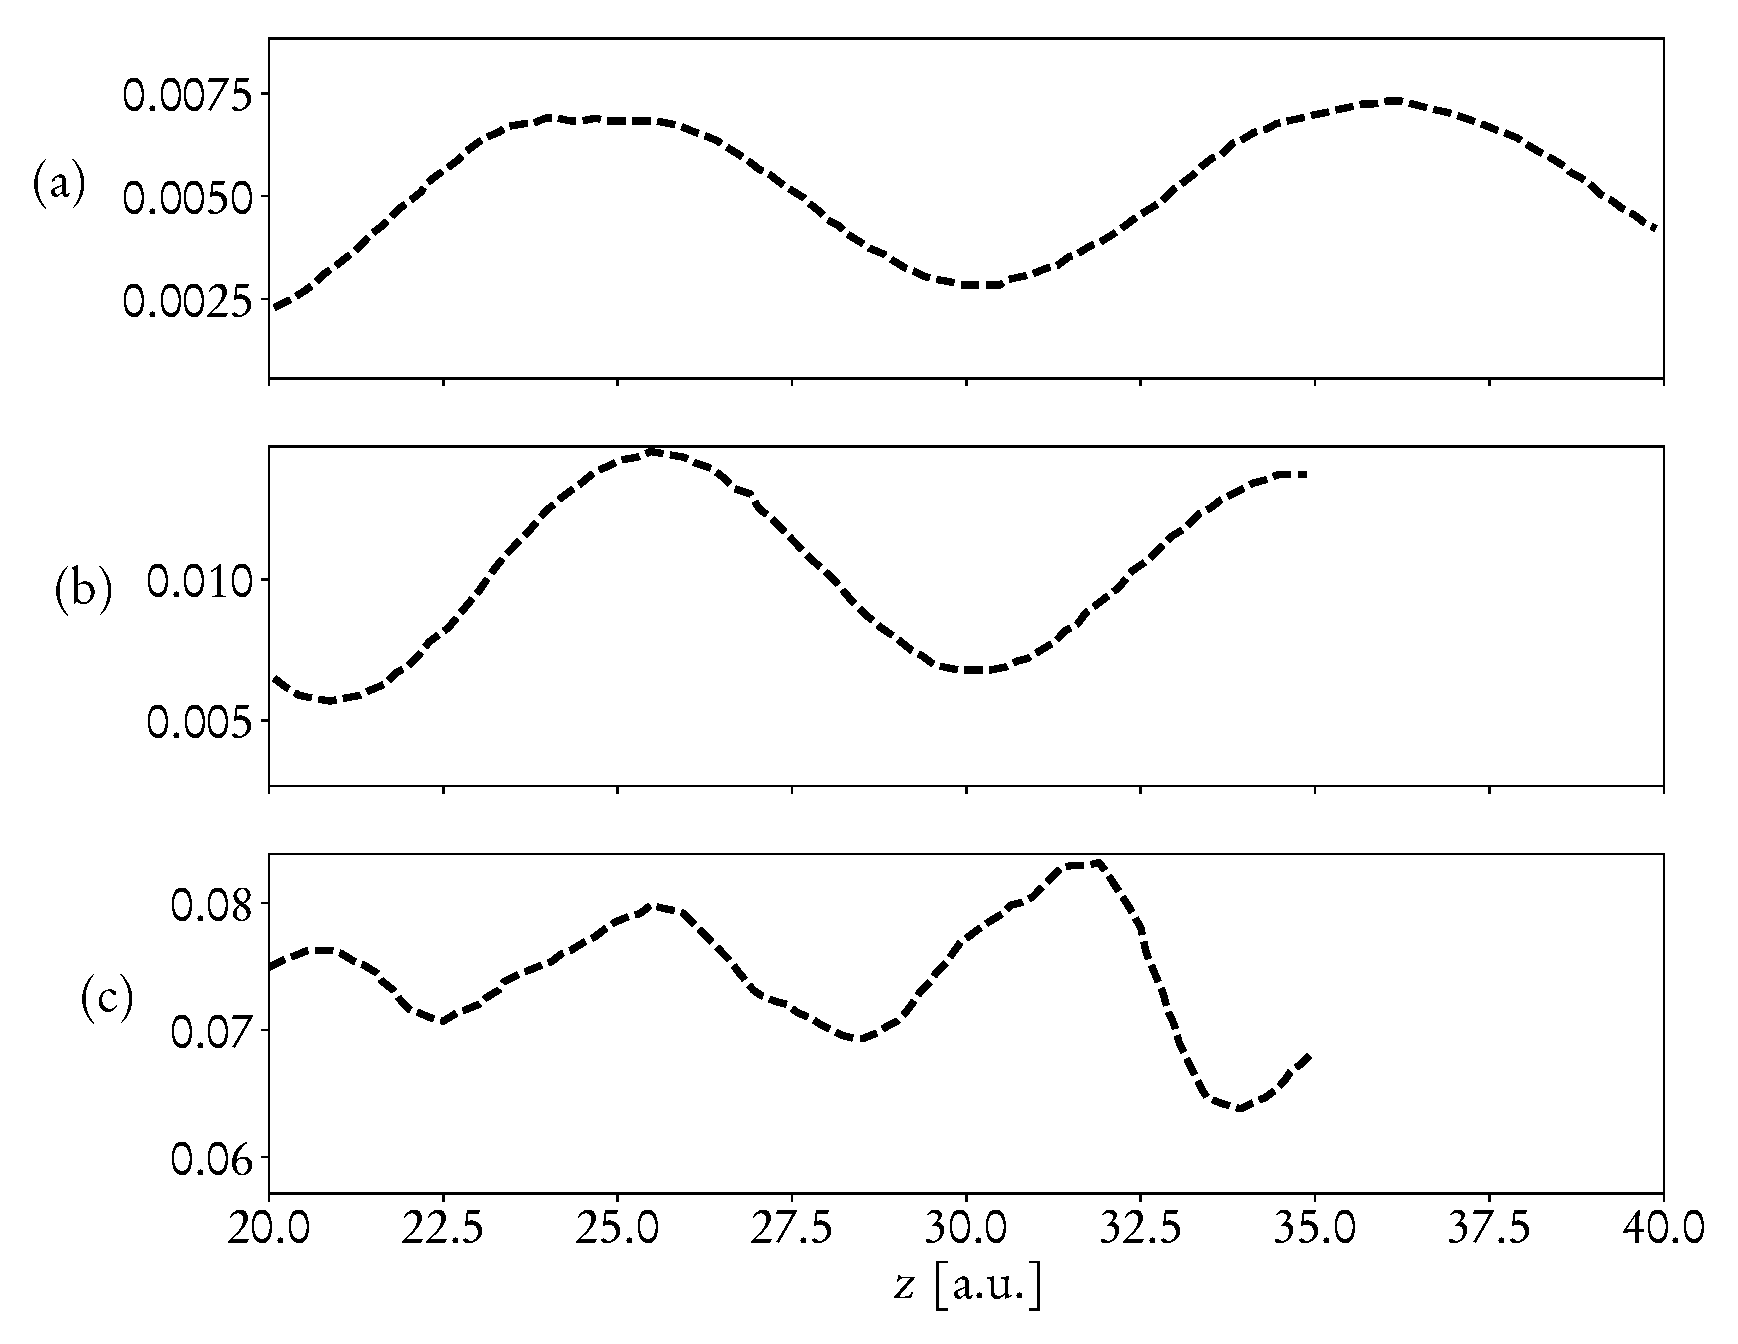
\includegraphics[width = \linewidth]{./images/poz.eps}
            \caption[Probabilities as a function of nuclear separation.]{$p^{II}$ as a
                     function of $z$, an impact energy of 50~keV, and impact parameter of 1~a.u.:
                     (a) $\bar{p}$-He, (b) $p$-He, (c) He\textsuperscript{2+}-He. \label{fig:poz}}
         \end{minipage} \hspace{0.009\linewidth} %
         \begin{minipage}{.49\linewidth}

            \centering
            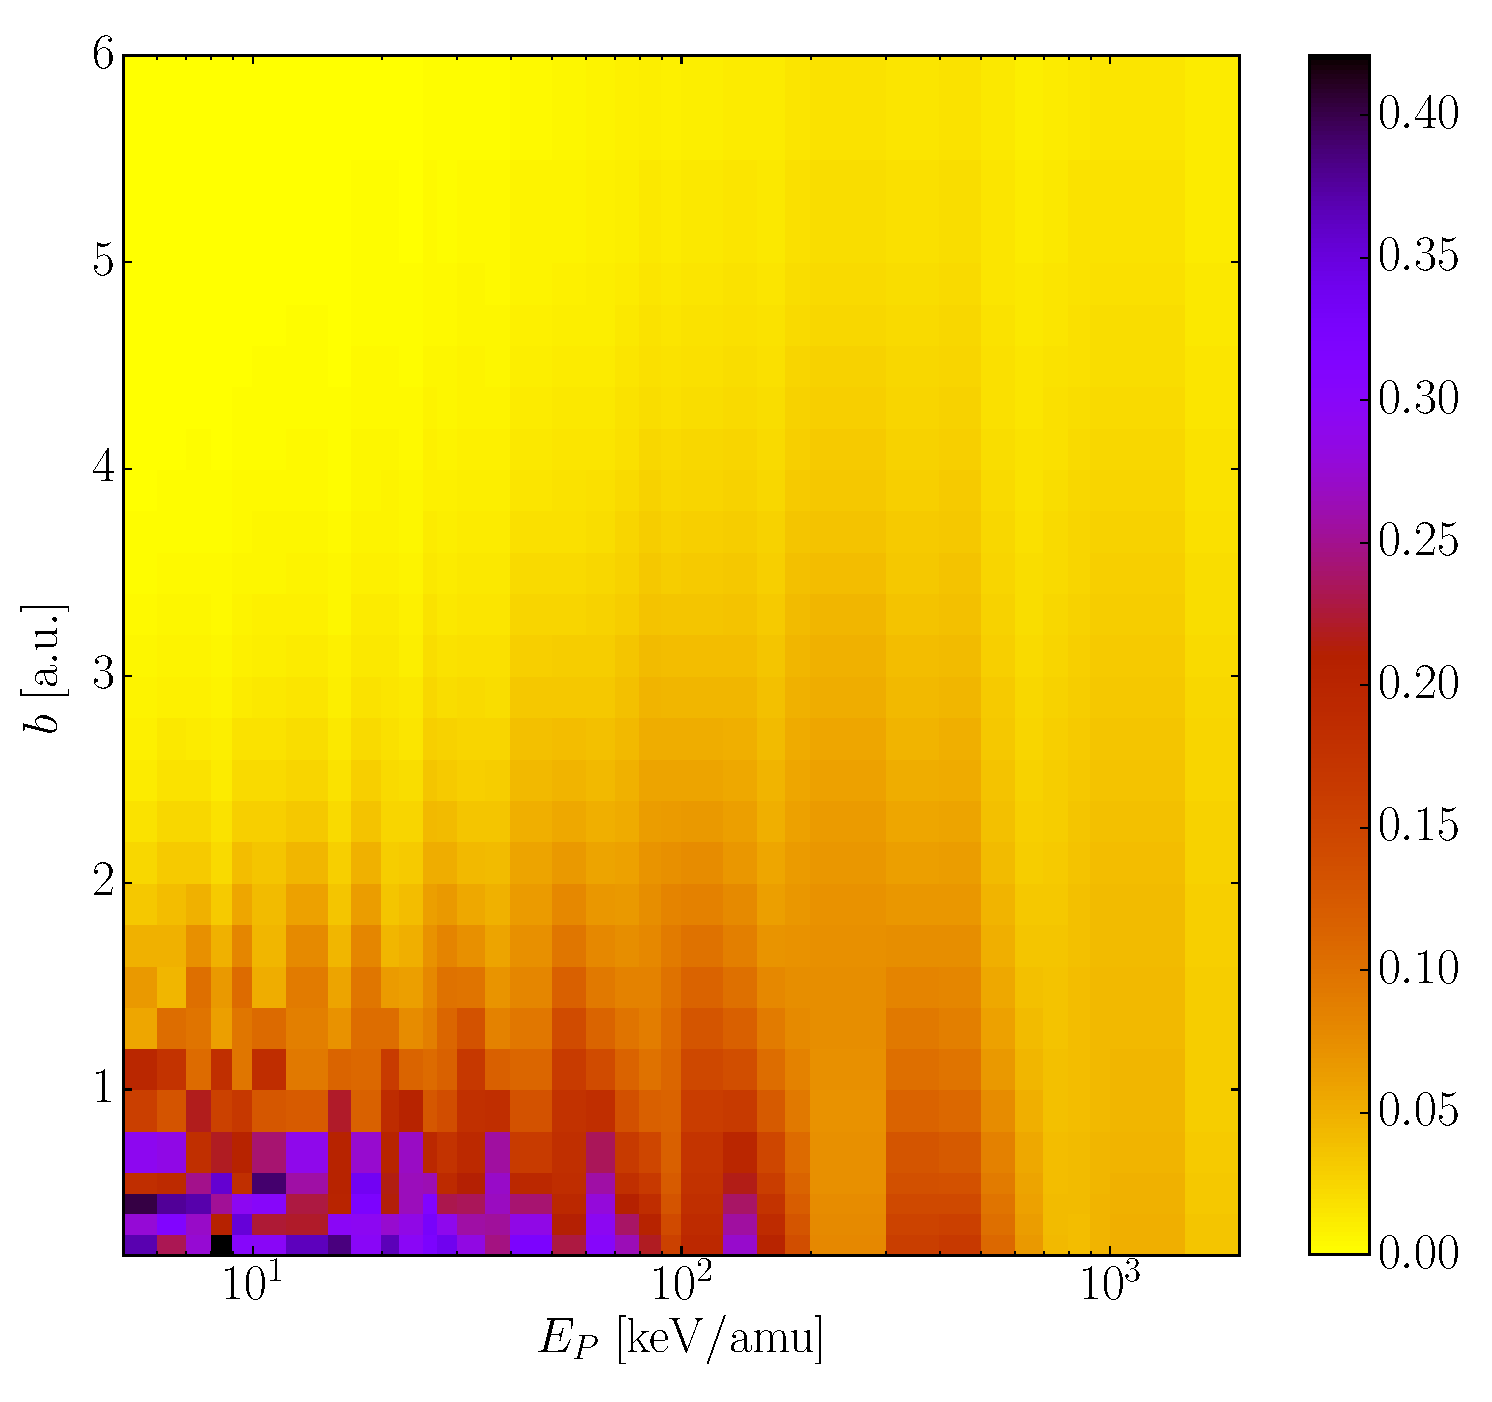
\includegraphics[width = \linewidth]{./images/dendiff.eps}
            \caption[Density difference]
                   {$\left| n_A(t_f) - n (t_f)\right|_1$ for the antiproton
                    helium collision system. \label{fig:l1}}
         \end{minipage}
      \end{figure}

      As has been discussed in previous works, for example~\cite{microresp,pbarhe}, fluctuations in the
      density persist after the collision process has completed if the Kohn-Sham potential is explicitly
      density dependent. Due to this fact the values of observables must be averaged over some range of
      $t_f$. The added complexity of the proton-helium collision system compared to that for
      antiproton-helium restricts the range through which the calculations may be run. Due to this fact
      an insufficient range of $t_f$ is available for averaging to produce a curve as smooth as in the
      $\bar{p}$-He system. More explicitly, letting $z_f = V t_f$ be the final target-projectile
      separation for impact velocity $V$, $\bar{p}$-He collisions may be run to a final separation of
      45~a.u., whereas $p$-He collisions run to a maximum inter-centre distance of around 35~a.u.

      Figure~\ref{fig:poz}, which depicts the values of $p^{II}$ as a function of $z$ for a prototypical
      choice of impact energy and parameter, makes these more apparent. Also of note is that the
      variances increase by about a factor of two between each of the collision systems.

      We can get a sense of how well the adiabatic density approximates the true time-dependent density
      at $t_f$ by considering their separation in function space. Owing to the fact that one-particle
      densities are necessarily $L^1$ functions (i.e.\ integrable functions) it is most natural to use
      the metric induced by the $L^1$-norm defined for any
      $f \in L^1\left(\mathbb{R}\right)$ by
      %
      \begin{equation} \label{eq:l1rorm}
         \left| f \right|_1 = \int \mathrm{d}^3 r \; \left| f(\mathbf{r}) \right|
      \end{equation}
      %
      for measuring this distance.

      Fig.~\ref{fig:l1} displays $\left| n(t_f) - n_A(t_f) \right|_1$, the difference between the
      adiabatic ($n_A$) and fully dynamic ($n$) densities at the final time $t_f$ for the
      antiproton-helium system\footnote{All integrals were performed with the aid of the \textsc{cuba}
      numerical integration package~\cite{cuba}.}. While it is possible to perform such an analysis for
      the $p$-He system as well added complications brought on by having to deal with a two centred
      system make it much more difficult to produce and analyze such data. Intuitively one would expect
      that the difference between the two densities should follow the single-particle probability $p_T$.
      This belief is supported by the easily derived relation
      %
      \begin{equation} \label{eq:diff-bound}
         \left| n(t_f) - n_A(t_f) \right|_1 \leq 4 p_T.
      \end{equation}
      %
      While Fig.~\ref{fig:p-ic} (which will be discussed in next section) demonstrates monotonic
      increase in $p_T$ with increasing impact parameter, a general trend for all impact energies,
      Fig.~\ref{fig:l1} contains additional structures. Also of note is the minimum that appears along
      the impact energy axis between 200 and 300~keV/amu. These unexpected features must be attributed
      to the fact that $n_A$ contains only trivial angular dependence which makes a proper description
      of excitation and partial removal of electronic density impossible. This provides indications of
      the limitations of the \textsc{wb} model.

   \end{section}

   \begin{section}{Results \label{sec:phe2p-res}}

      In the following subsections we present several plots of total cross sections for a variety of
      collision processes. Given an outcome probability $p_\mathrm{outcome}$ the total cross section
      associated with this probability is determined according to
      %
      \begin{equation} \label{eq:tcs}
         \sigma_\mathrm{outcome} = \int \mathrm{d}^2 b \, p_\mathrm{outcome} (\mathbf{b})
         = 2 \pi \int^\infty_0 \mathrm{d}b \; b \, p_\mathrm{outcome} (b).
      \end{equation}

      We will refer to our results using the acronyms \textsc{iem} and \textsc{wb} corresponding to
      probabilities calculated using Eq.~\eqref{eq:prob-iem} and Eq.~\eqref{eq:prob-ic} using the
      \textsc{wb} model respectively. In both cases the dynamics include the frozen \textsc{mchf}
      ground-state correlation potential.

      The figures presented below were generated with several criteria in mind. First, a minimal number
      of older calculations was selected with the aim of covering as much of the impact energy range as
      possible while avoiding over burdening the figures with multiple overlapping curves. Second, works
      chosen must be the product of calculations that go beyond an \textsc{iem} description of the
      collision process with preference given to fully correlated two-electron calculations. If one is
      interested in some of the calculations excluded from these comparisons there exist a plethora of
      independent electron, independent event, or related models~\cite{SLD-83, DMR-84, SLD-85, GM-86,
      CM-87, GM-87, JLF-89, DC-90, DC-91a, DC-91b, DG-91, SKG-91, SL-91, Kuang-92, MLC-93, CM-94,
      CSR-95, BDM-96, MBGH-97, McCartney-97, Mccartney-99, GAMRF-02, GFS-02, AMRF-04, BLMC-04, FRBJG-06,
      FJG-07, GIFK-08, ZK-09, G-11, LFG-11, GG-12a}, classical trajectory Monte Carlo
      calculations~\cite{ZM-85, OWM-86, MO-87, WO-88, MS-89, Cohen-96, TH-96, MMTH-02, DAKW-04, GEP-09},
      and other classical statistical models such as the Bohr-Lindhard model~\cite{DYC-08,Ding-12} for
      one to consider at their own leisure.

      \begin{subsection}{ \texorpdfstring{$\bar{p}$}{pbar}-He Vs. \texorpdfstring{$p$}{p}-He Collisions
                         \label{sec:pbarhe-res}}

         \begin{figure}[t]
            \centering
            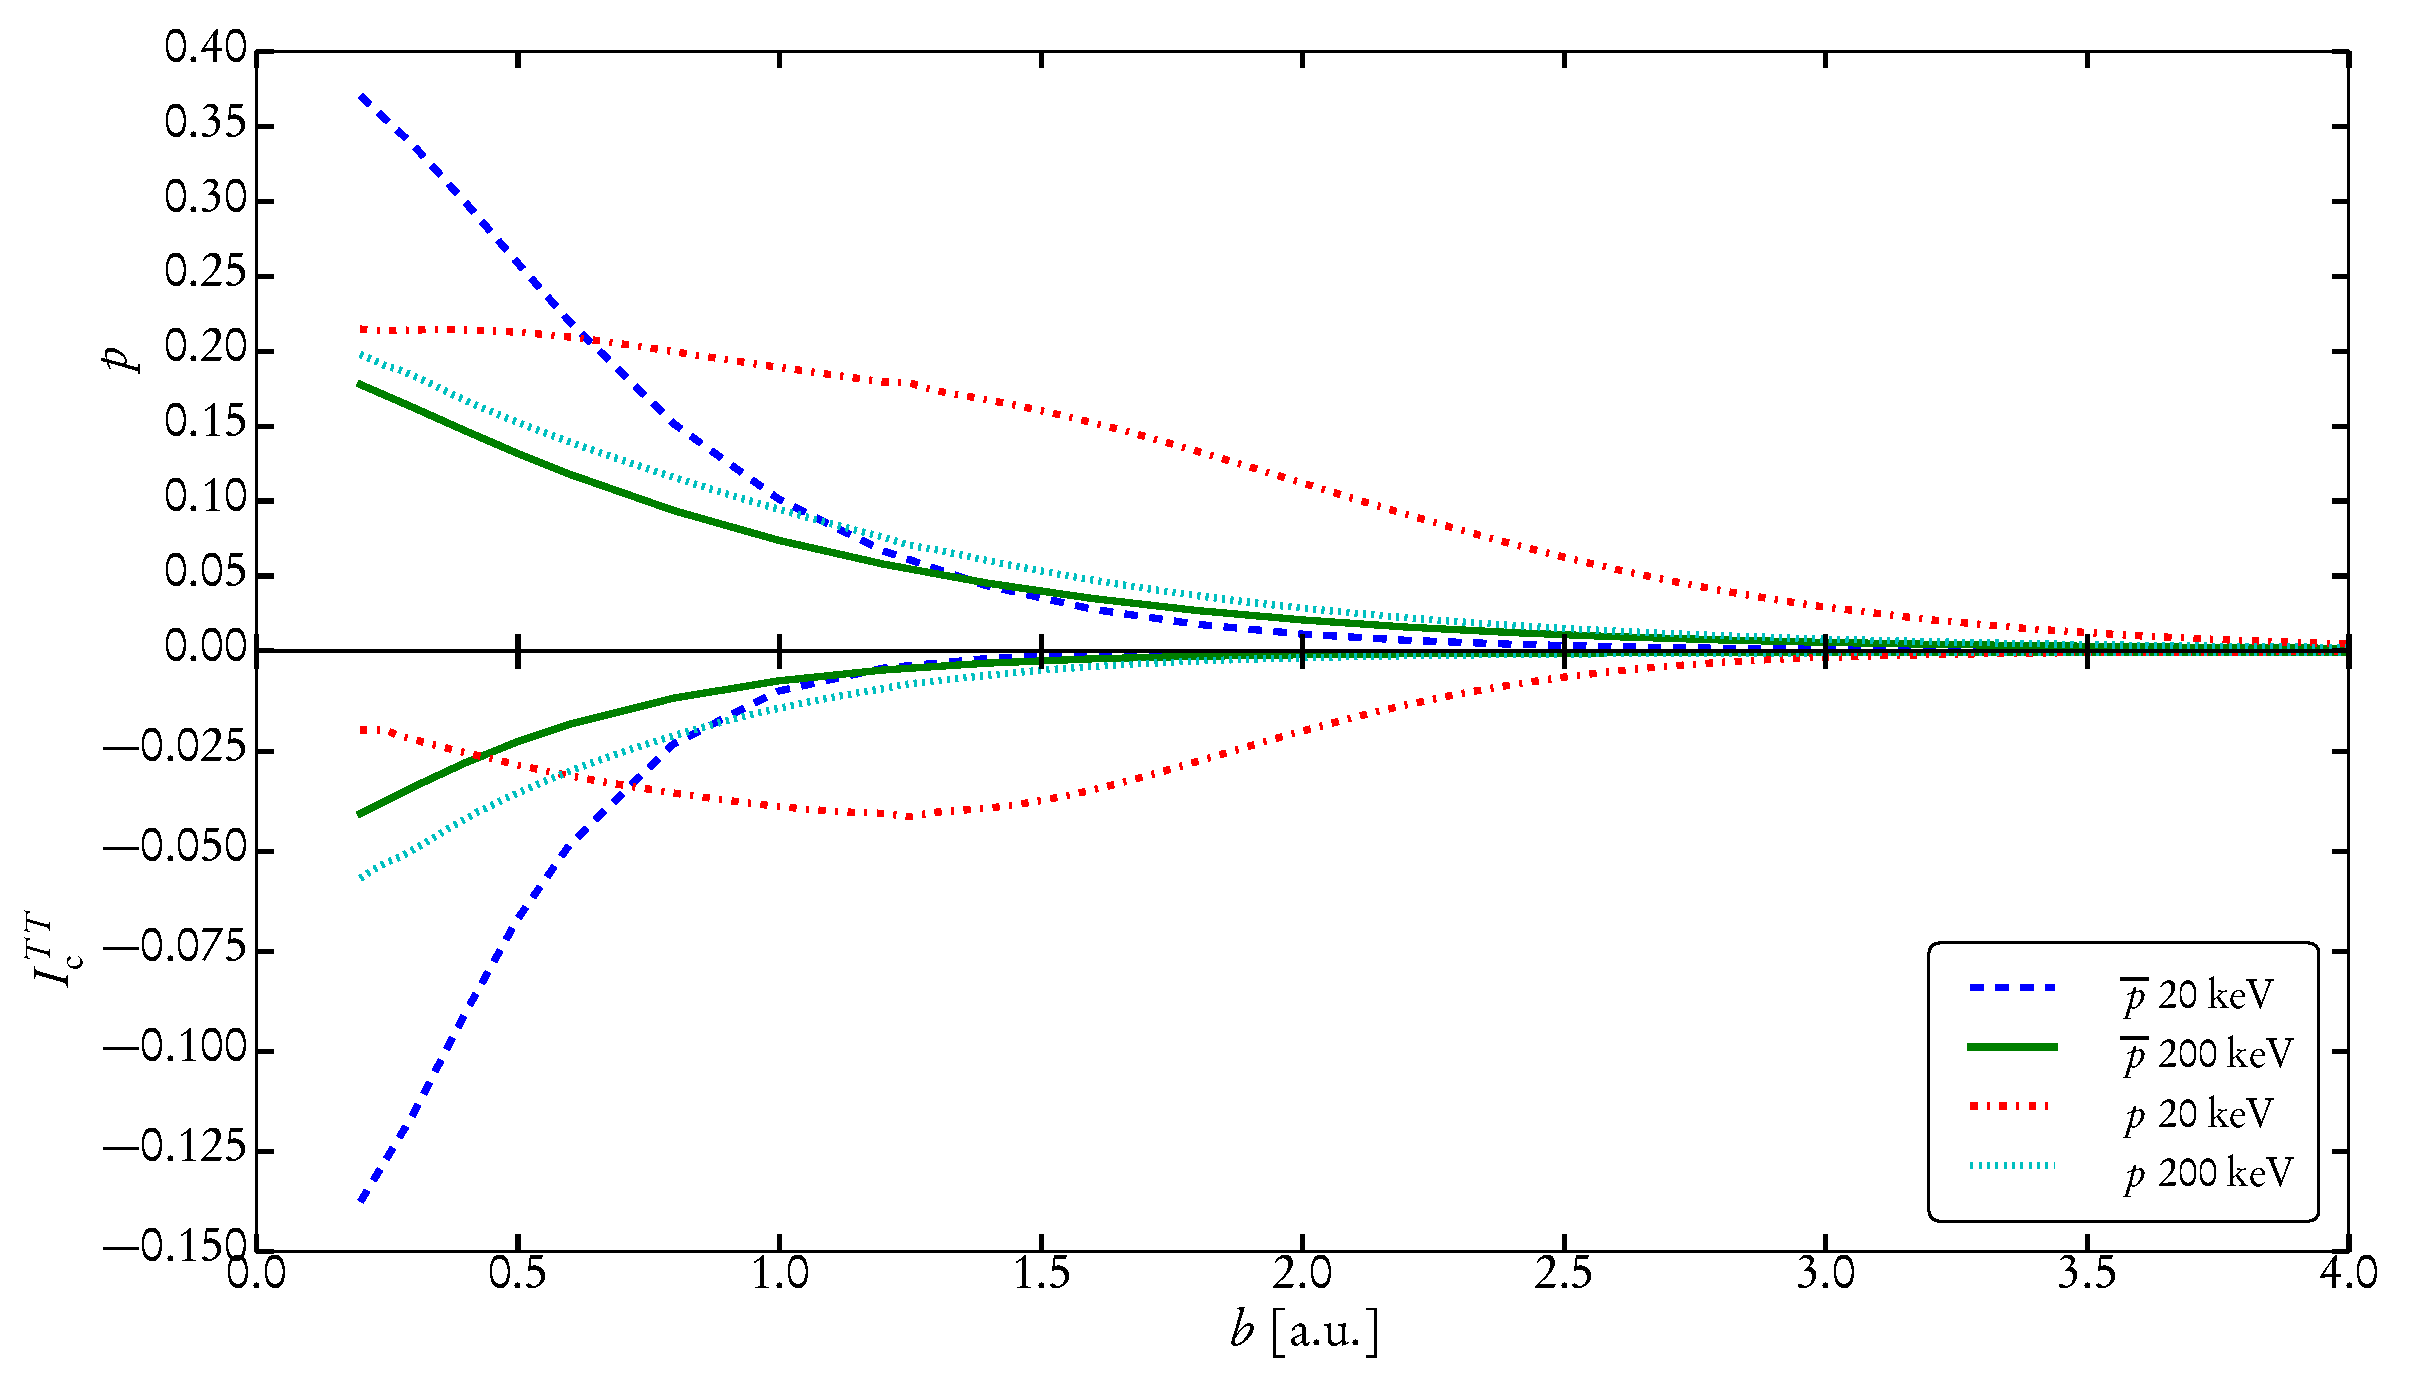
\includegraphics[width = 0.95 \linewidth]{./images/p-ic.eps}
            \caption[Single-particle removal and correlation integral]
                    {Single-particle removal probability, $p$, (upper pane) and
                     correlation integral, $I_\mathrm{c}^{TT}$, (lower pane) as functions of impact
                     parameter for antiprotons and protons incident on helium atoms at 20 and
                     200~keV/amu. \label{fig:p-ic}}
         \end{figure}

         \begin{figure}[t]
            \centering
            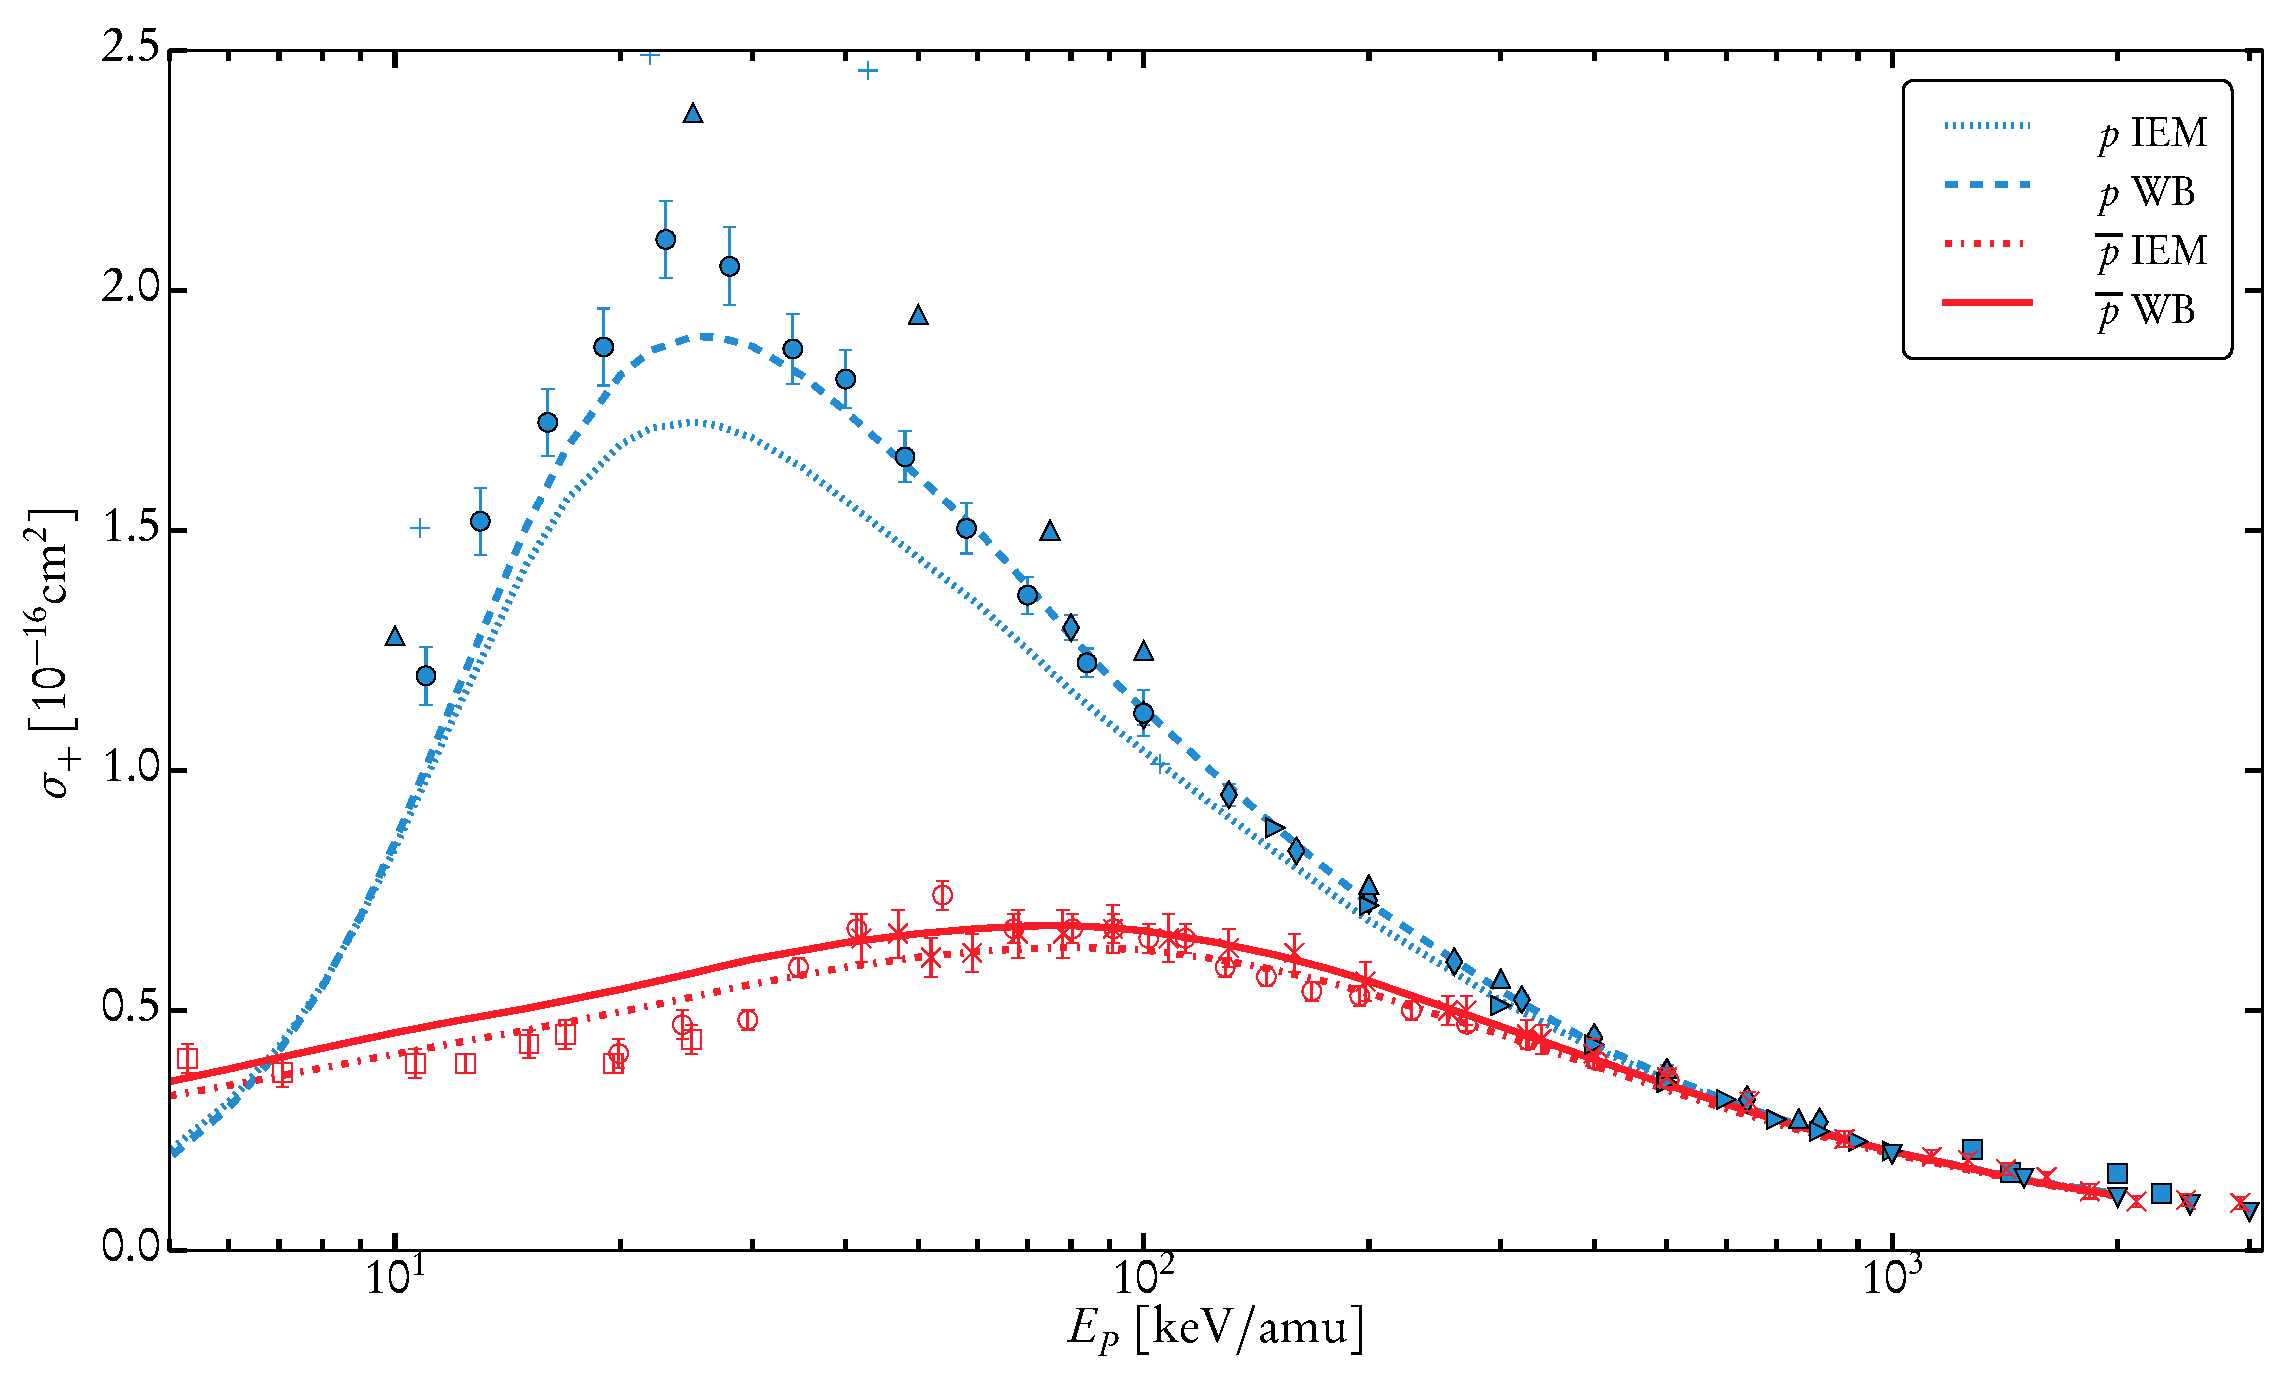
\includegraphics[width = 0.95 \linewidth]{./images/pbarhe/pbarhe-+.eps}
            \caption[Total cross section for one-electron removal from helium by protons and
                     antiprotons.]
                    {Total cross section for one-electron removal from helium by protons and
                     antiprotons. Protons: dotted \textsc{iem} and dashed \textsc{wb} (theory);
                     {\color{blue}{$\blacktriangle$}}~\cite{DTR84}, {\color{blue}{$+$}}~\cite{Sol62},
                     {\color{blue}{$\bullet$}}~\cite{SG89}, {\color{blue}{$\blacklozenge$}}~\cite{SG85},
                     {\color{blue}{$\blacktriangleright$}}~\cite{PM70},
                     {\color{blue}{$\blacktriangledown$}}~\cite{Wex64},
                     and {\color{blue}{$\blacksquare$}}~\cite{KAH84} (experiment).
                     Antiprotons: dashed-dotted \textsc{iem} and solid \textsc{wb} (theory);
                     {\color{red}{$\Box$}}~\cite{KKT08}, {\color{red}{$\circ$}}~\cite{HKM94},
                     and {\color{red}{$\times$}}~\cite{AHK90} (experiment). \label{fig:he+}}
         \end{figure}

         \begin{figure}[t]
            \centering
            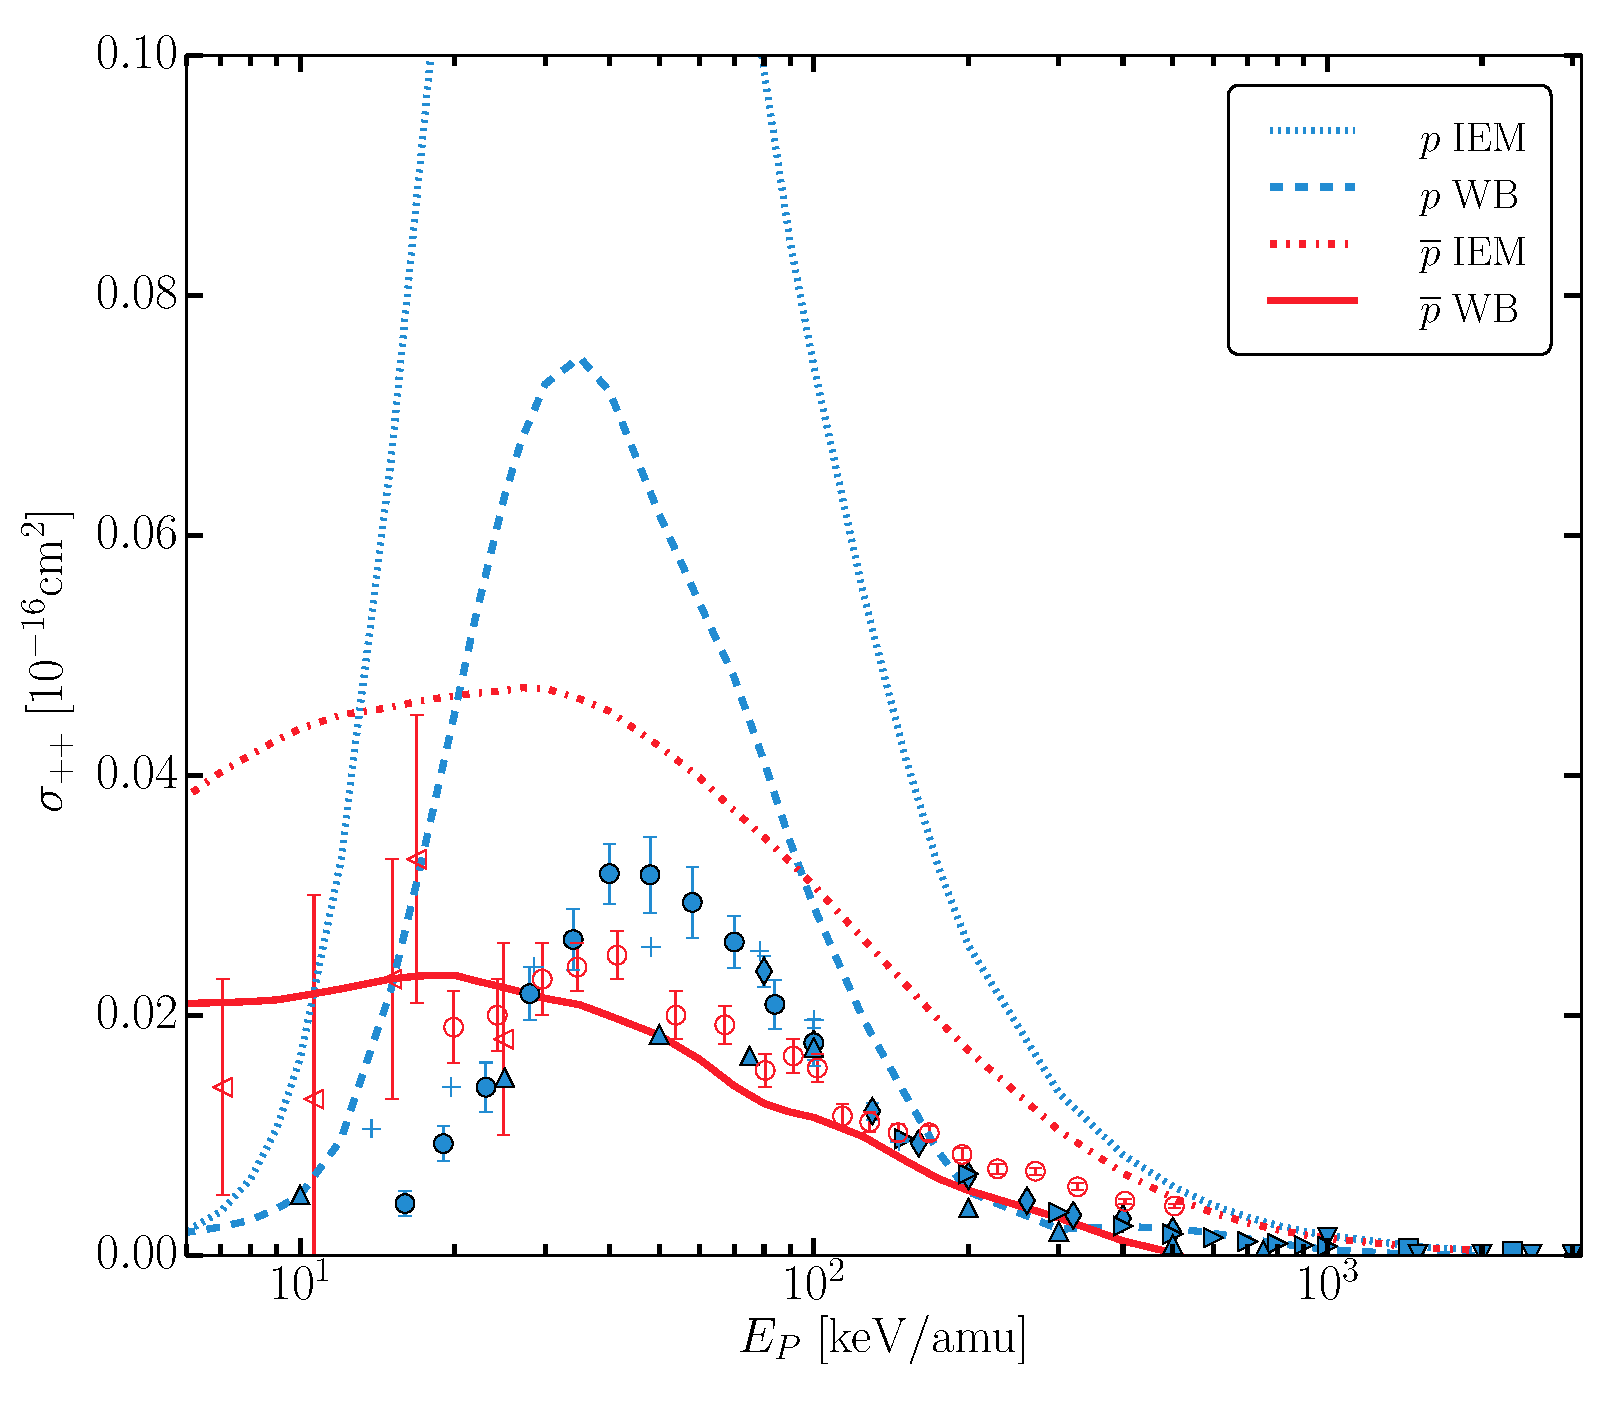
\includegraphics[width = 0.95 \linewidth]{./images/pbarhe/pbarhe-++.eps}
            \caption[Total cross section for two-electron removal from helium atoms as a function of
                     impact energy]
                    {Total cross section for two-electron removal from helium atoms as a function
                     of impact energy. Protons: dotted \textsc{iem} and dashed \textsc{wb} (theory);
                     {\color{blue}{$\blacktriangle$}}~\cite{DTR84}, {\color{blue}{$+$}}~\cite{Sol62},
                     {\color{blue}{$\bullet$}}~\cite{SG89},
                     {\color{blue}{$\blacklozenge$}}~\cite{SG85},
                    {\color{blue}{$\blacktriangleright$}}~\cite{PM70},
                    {\color{blue}{$\blacktriangledown$}}~\cite{Wex64}, and
                    {\color{blue}{$\blacksquare$}}~\cite{KAH84} (experiment).
                    Antiprotons: dashed-dotted \textsc{iem} and solid \textsc{wb} (theory);
                    {\color{red}{$\circ$}}~\cite{HKM94} and {\color{red}{$\triangleleft$}}~\cite{KKT09}
                       (experiment). \label{fig:he++}}
         \end{figure}

         We begin the analysis of results with a comparison of proton and antiproton collisions with
         helium. To facilitate juxtaposition we will consider the zero-, one-, and two-electron removal
         processes in aggregate. The probabilities for these outcomes are given respectively by
         %
         \begin{subequations} \label{eq:remove}
            \begin{equation} \label{eq:rem-0}
               p_0 = (1 - p)^2 + \tfrac{1}{2} I^{TT}_\mathrm{c} = p^{TT},
            \end{equation}
            %
            \begin{equation} \label{eq:rem-1}
               p_+ = 2 p (1-p) - I^{TT}_\mathrm{c} = p^{TI} + p^{TP},
            \end{equation}
            %
            \begin{equation} \label{eq:rem-2}
               p_{++} = p^2 + \tfrac{1}{2} I^{TT}_\mathrm{c} = p^{II} + p^{IP} + p^{PP},
            \end{equation}
         \end{subequations}
         %
         where the single-particle removal probability is given by
         %
         \begin{equation} \label{eq:p-rem}
            p = 1 - \tfrac{1}{2} \int_T \mathrm{d}^3 r \; n(\mathbf{r},t_f)
            = 1 - p_T = p_P + p_I.
         \end{equation}
         %
         For the $\bar{p}$-He system these are simply the probabilities presented in
         Eq.~\eqref{eq:prob-pbarhe} making this choice of observables ideal for contrasting with the
         $p$-He system.

         Presented in Fig.~\ref{fig:p-ic} are the single-particle removal probability and
         $I^{TT}_\mathrm{c}$ for both the proton and antiproton collision systems at 20 and 200~keV/amu
         as functions of the impact parameter. The correlation integral is always negative, decaying to
         zero in increasingly distant collisions as electron removal becomes less likely. This means
         that it provides a blanket enhancement to one-electron removal processes
         [cf.\ Eq.~\eqref{eq:rem-1}].

         At 200~keV/amu the results for both $p$ and $I^{TT}_\mathrm{c}$ become similar; at lower
         energies (i.e., 20~keV/amu) there are significant differences for proton and antiproton
         collisions. In this range the single-removal probability for antiprotons decays swiftly with
         rising impact parameter. On the other hand, the single-particle removal probability in low
         energy proton-helium collisions remains appreciable over a much larger range. Such impact
         parameter profiles are a signature of electron capture which is the dominant electron removal
         process at lower impact energies. This behaviour is mirrored by that of $I^{TT}_\mathrm{c}$.

         A final feature of note is the spike in both antiproton curves at low impact parameter. In this
         region the antiproton passes through the charge density of the helium atom. Such close
         approaches result in destabilization of the electron binding and very efficient
         ionization~\cite{pbarhe-rev}

         Figures~\ref{fig:he+} and~\ref{fig:he++} present the total cross sections for one- and
         two-electron removal as functions of impact energy. These plots compare only the current
         proton-helium collision results to an updated version (denser impact energy grid and larger
         range of averaging as described in Sec.~\ref{sec:phe2p-det}) of the antiproton-helium results
         of~\cite{pbarhe} and to experimental data. For a comparison with other theoretical work
         see~\cite{thesis} (or~\cite{pbarhe}) and~\cite{new-pbarhe} ($\bar{p}$-He) and
         Sec.~\ref{sec:phe-res} ($p$-He).

         For one-electron removal, Fig.~\ref{fig:he+}, the \textsc{wb} model provides an increase for
         both protons and antiprotons over the \textsc{iem} except at higher energies where the
         correlation integral tends to be small in magnitude as indicated by Fig.~\ref{fig:p-ic}. In the
         case of proton-helium collisions this increase is an obvious improvement. The spread of the
         experimental data for antiproton-helium collisions makes it difficult to ascertain whether the
         enhancement in the cross section is preferable.

         The two-electron removal cross sections, Fig.~\ref{fig:he++}, for both proton and antiproton
         collisions are reduced significantly by the \textsc{wb} model. These reductions represent a
         clear improvement in either case. While the antiproton results are in fair agreement with
         experiment through the entire range explored the proton-helium results still differ notably
         below impact energies of 100~keV/amu. This is an indication that the \textsc{wb} model begins
         to display problems as capture becomes more important. These issues will be discussed in
         greater detail in the proceeding subsections.

      \end{subsection}

      \begin{subsection}{\texorpdfstring{$p$}{p}-He Collisions \label{sec:phe-res}}

         \begin{figure}[t]
            \centering
            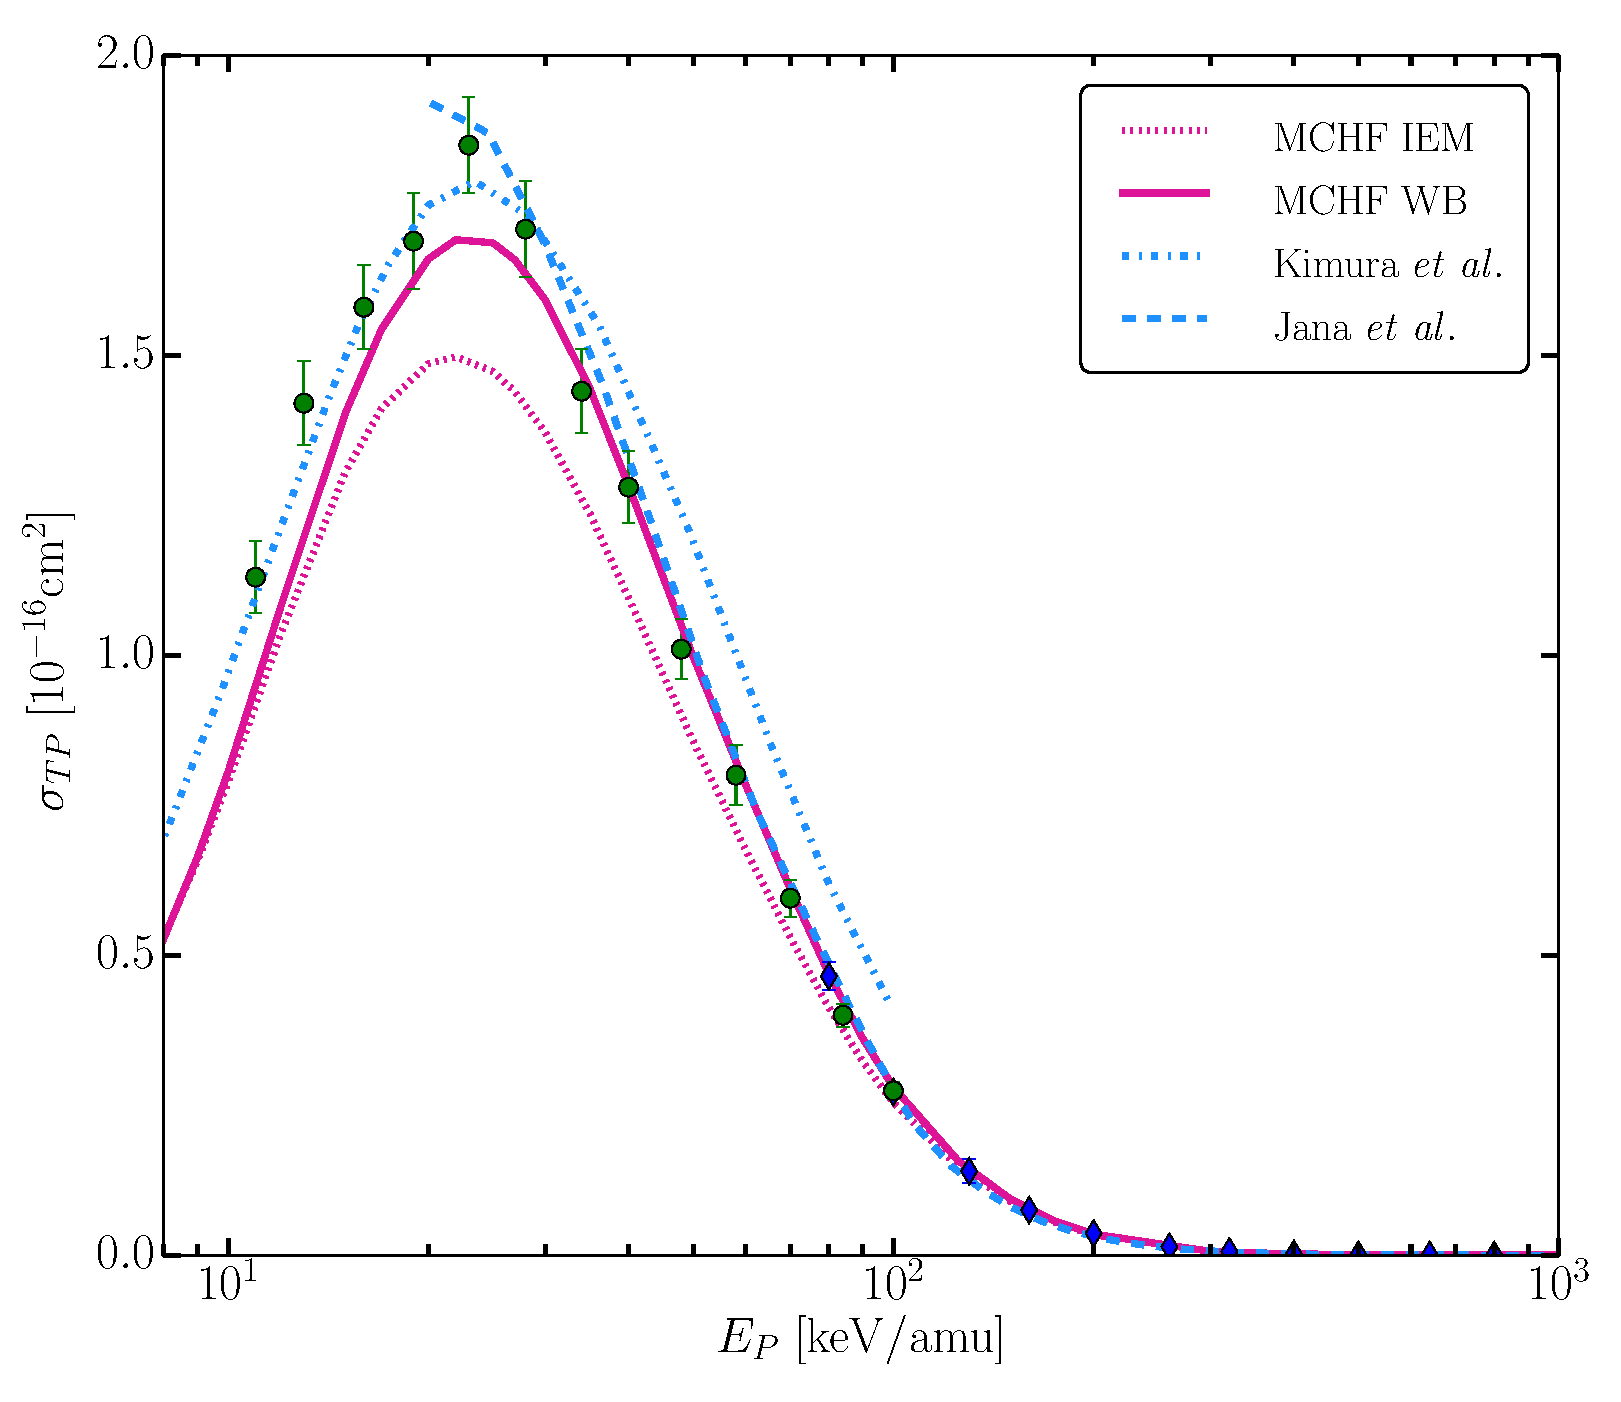
\includegraphics[width = 0.95 \linewidth]{./images/phe/phe-TP.eps}
            \caption[Total cross section for single capture in proton-helium collisions.]
                    {Total cross section for single capture in proton-helium collisions.
                     Theoretical results: \textsc{ao-mo} model of Kimura et al.~\cite{KL-86} and
                     \textsc{dw-4b} (post form) of Jana et al.~\cite{JMP-15}. Experimental Data:
                     {\color{OliveGreen}{$\bullet$}}~\cite{SG89} and
                     {\color{blue}{$\blacklozenge$}}~\cite{SG85}. \label{fig:phe-tp}}
         \end{figure}

         \begin{figure}[t]
            \centering
            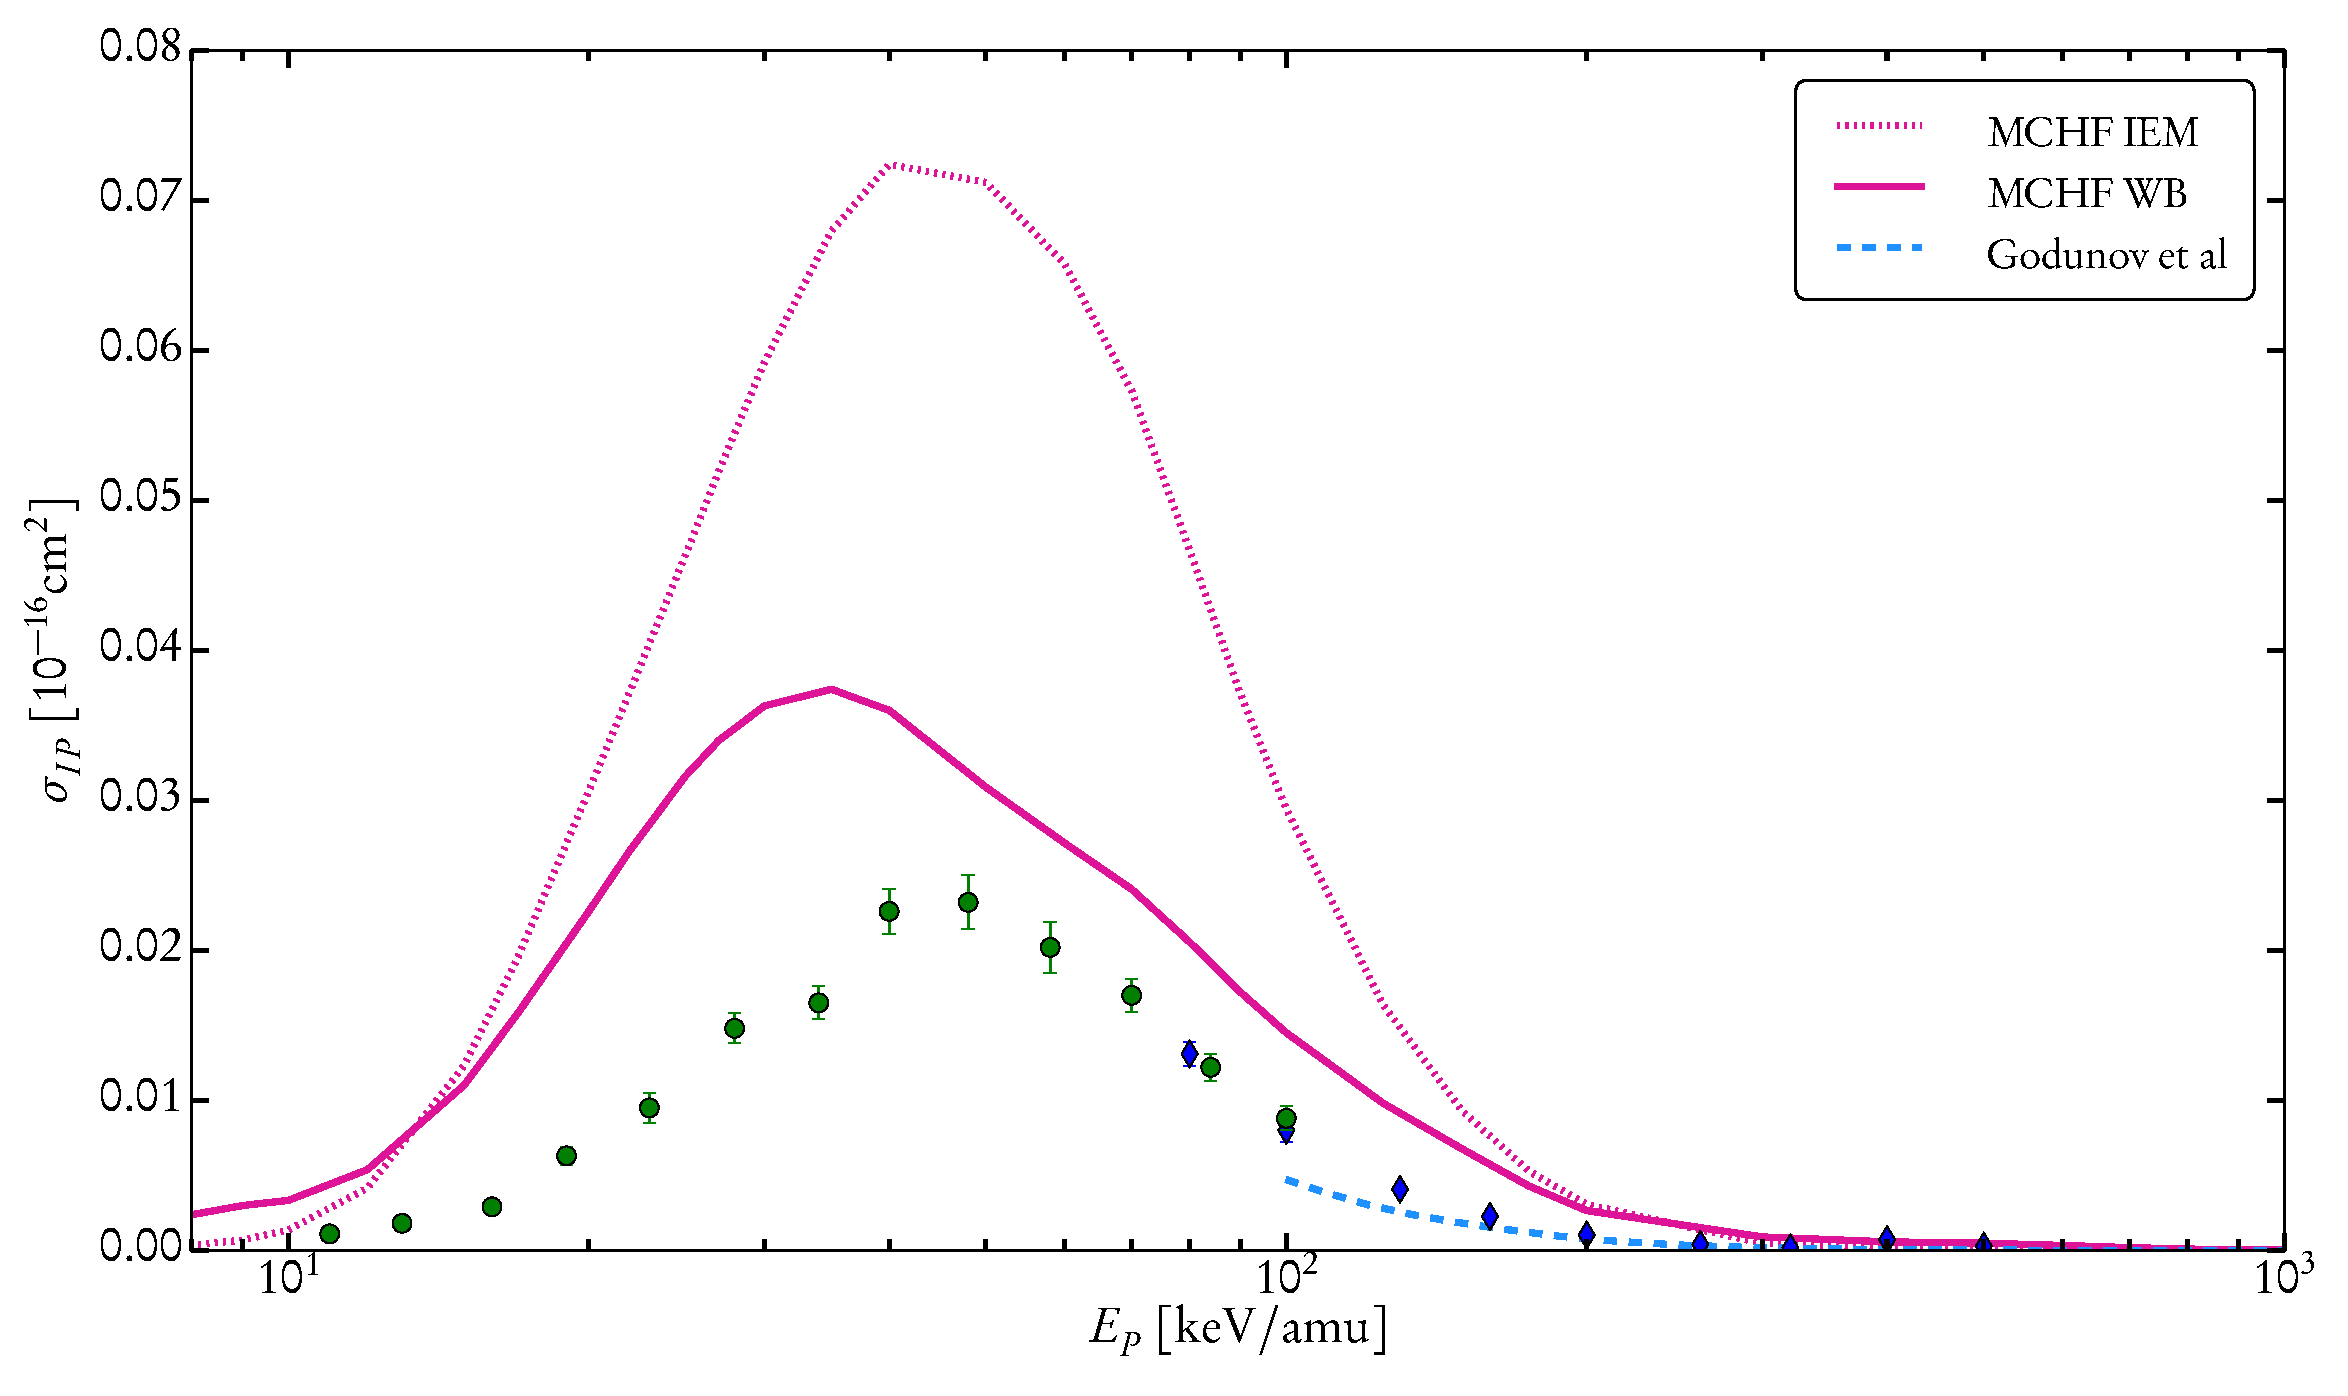
\includegraphics[width = 0.95 \linewidth]{./images/phe/phe-IP.eps}
            \caption[Total cross section for transfer ionization in proton-helium collisions.]
                    {Total cross section for transfer ionization in proton-helium collisions.
                     Theoretical results: Second order Born approximation of Godunov
                     et al.~\cite{Godunov-06}. Experimental data:
                     {\color{OliveGreen}{$\bullet$}}~\cite{SG89} and
                     {\color{blue}{$\blacklozenge$}}~\cite{SG85}. \label{fig:phe-ip}}
         \end{figure}

         \begin{figure}[t]
            \centering
            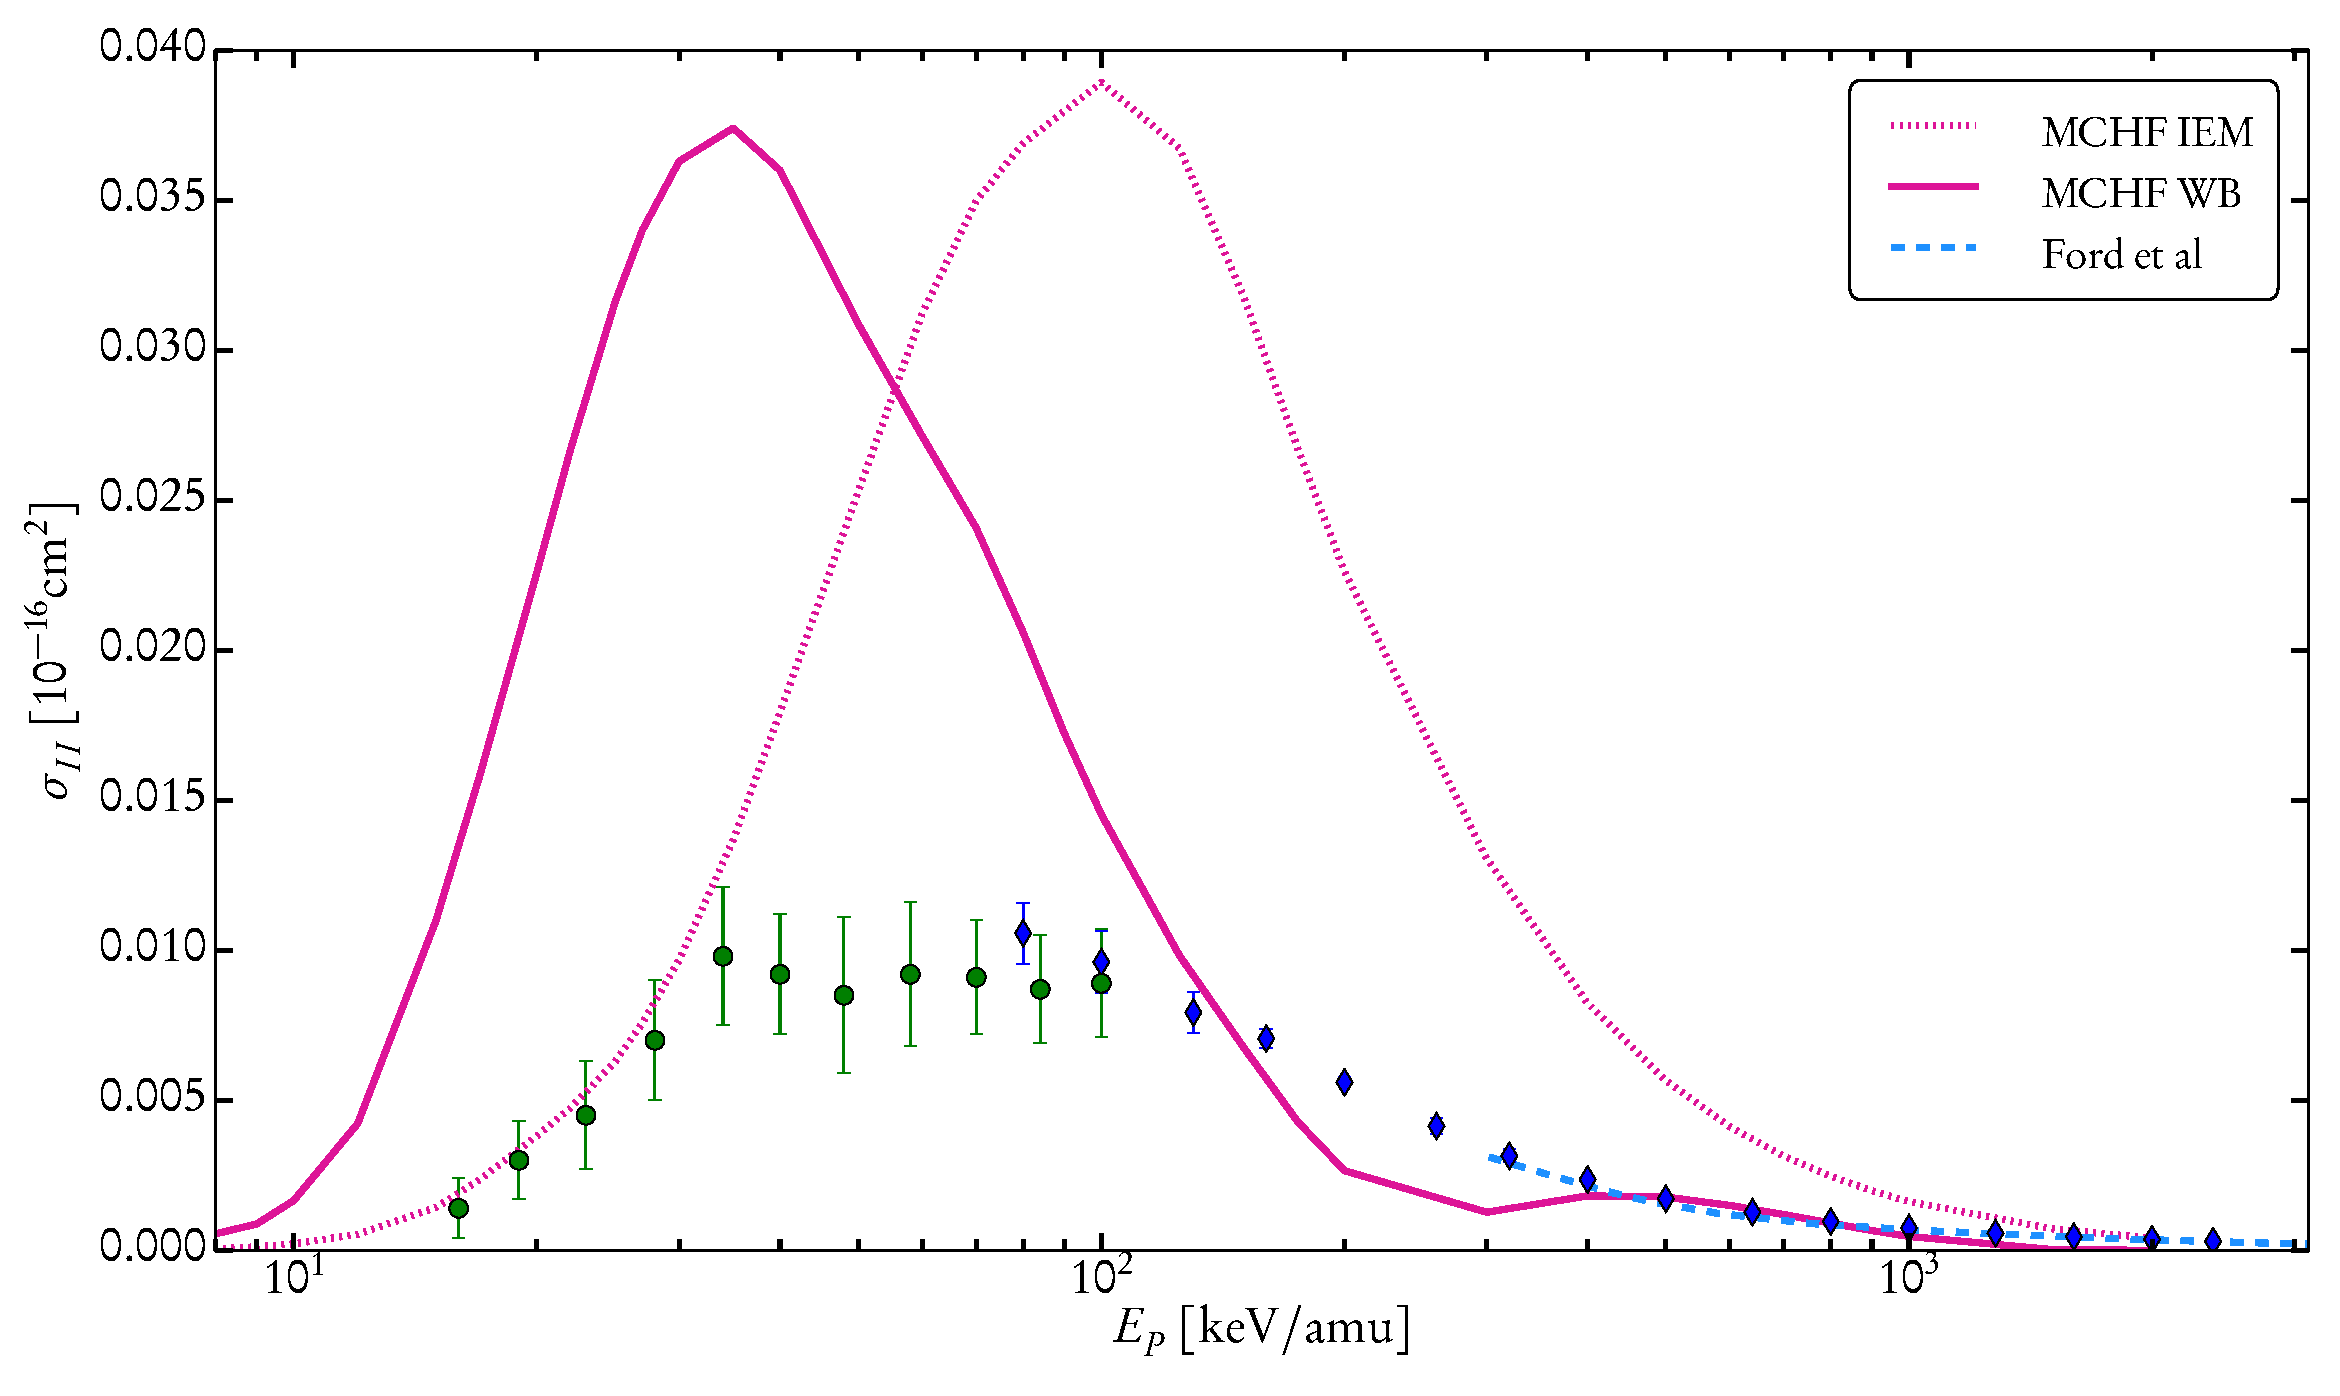
\includegraphics[width = 0.95 \linewidth]{./images/phe/phe-II.eps}
            \caption[Total cross section for double ionization of helium by proton impact.]
                    {Total cross section for double ionization of helium by proton impact.
                     Theoretical results: \textsc{fim} of Ford et al.~\cite{FR-94}.
                     Experimental data: {\color{OliveGreen}{$\bullet$}}~\cite{SG89} and
                     {\color{blue}{$\blacklozenge$}}~\cite{SG85}. \label{fig:phe-ii}}
         \end{figure}

         \begin{figure}[t]
            \centering
            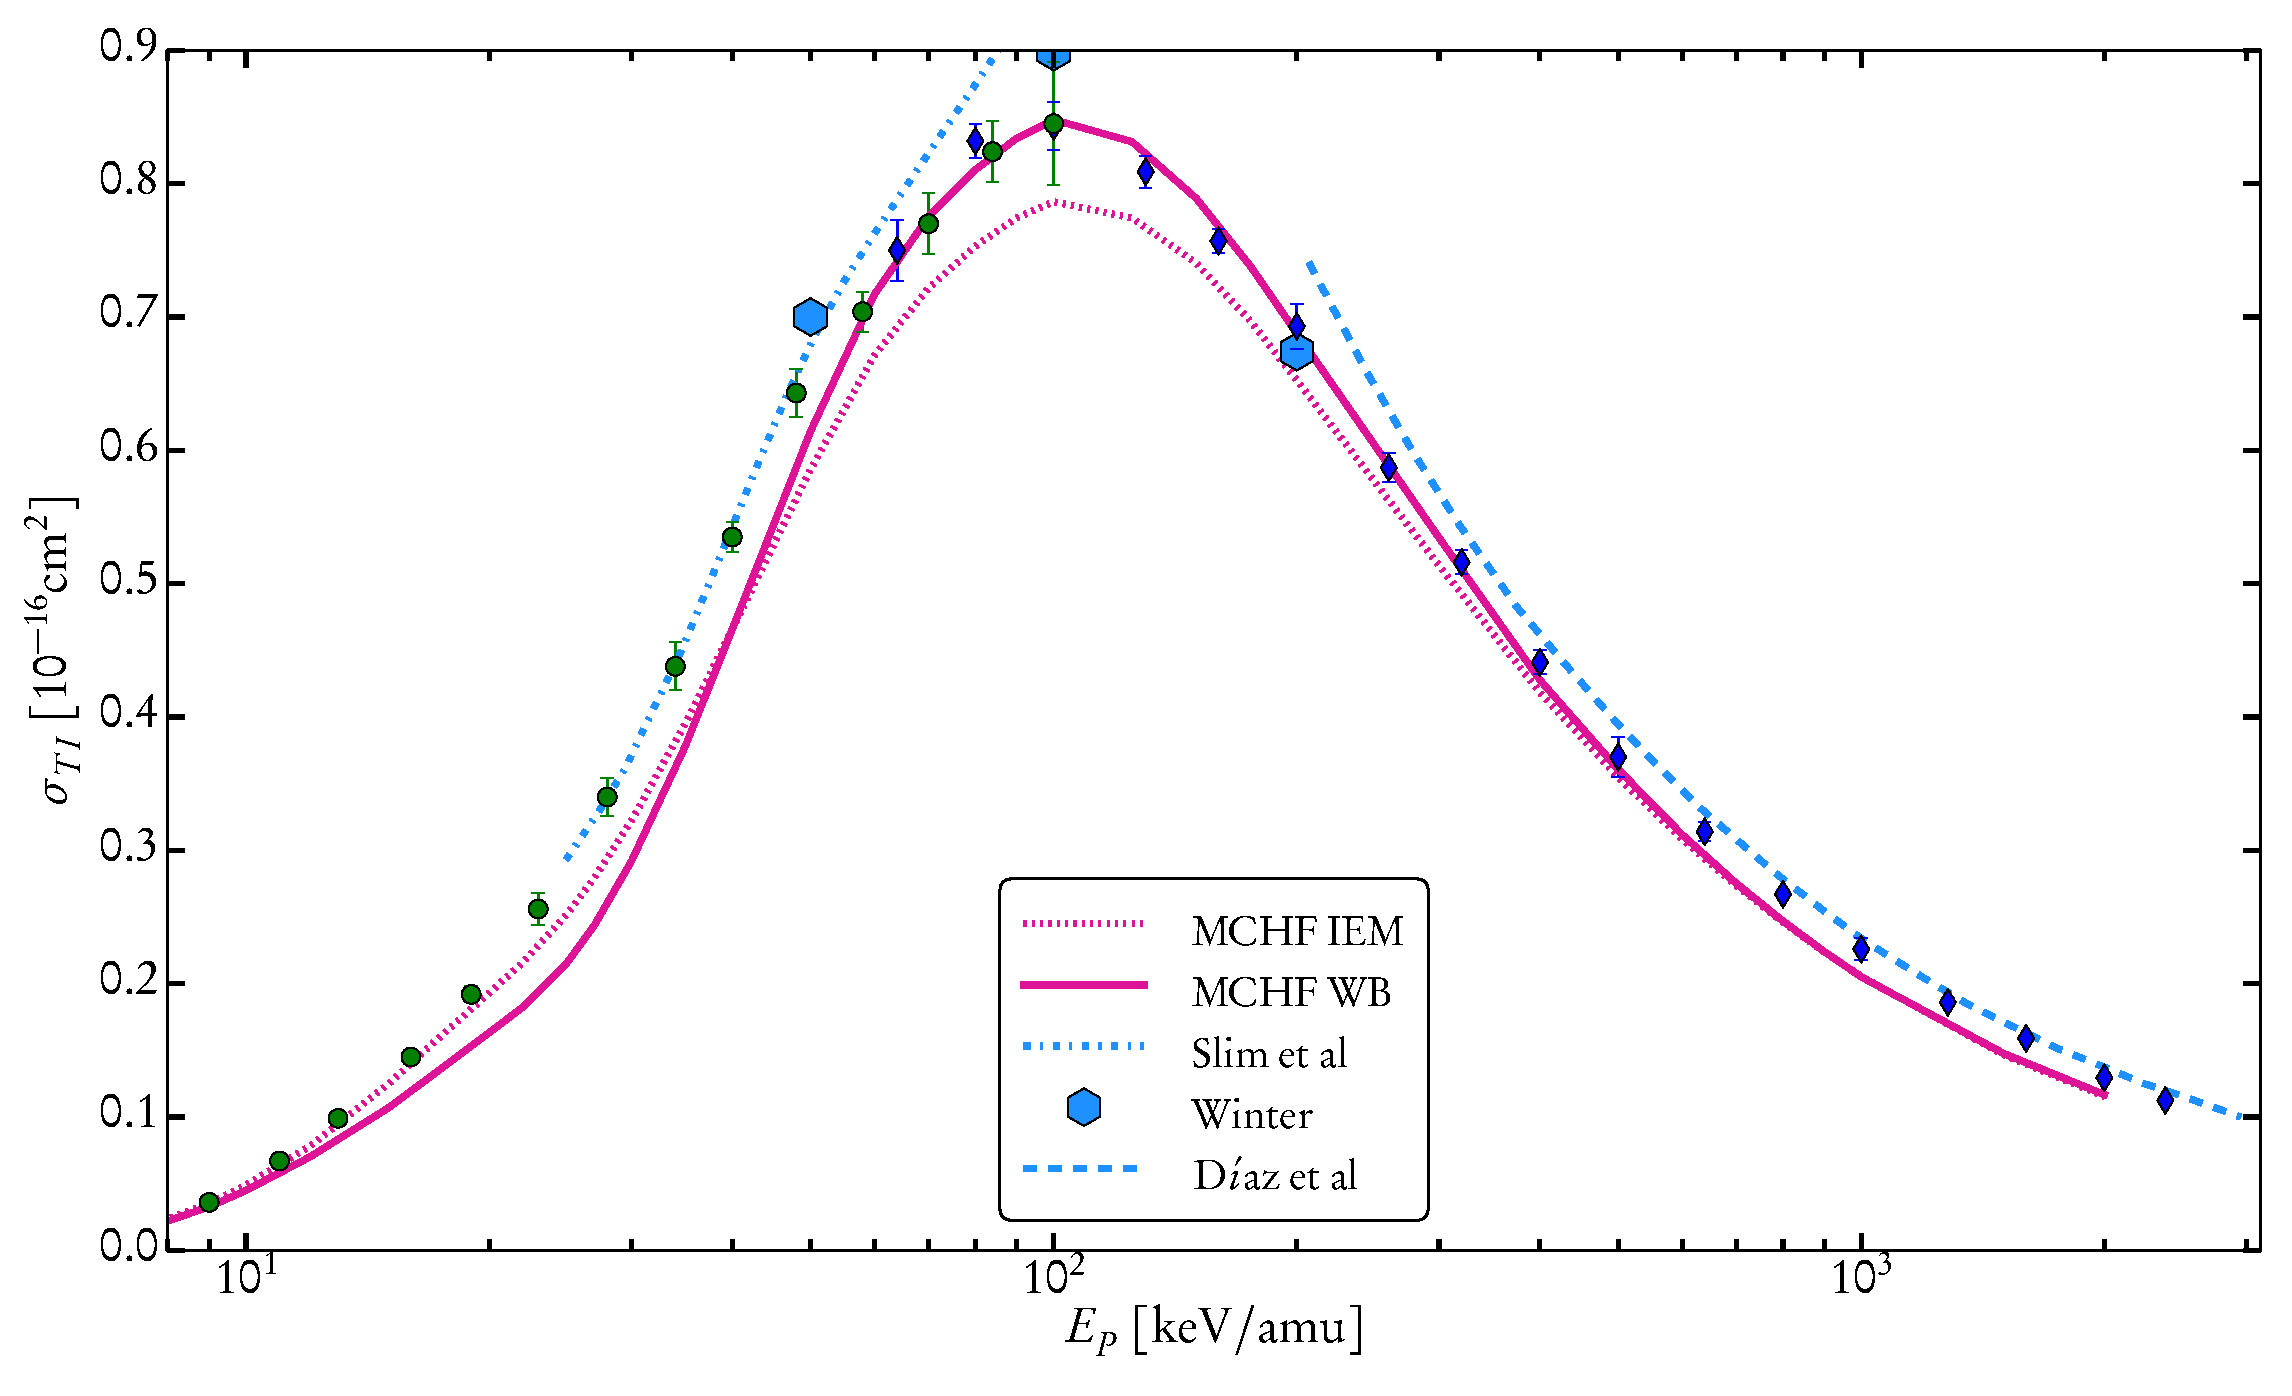
\includegraphics[width = 0.95 \linewidth]{./images/phe/phe-TI.eps}
            \caption[Total cross section for single ionization of helium by proton impact.]
                    {Total cross section for single ionization of helium by proton impact.
                     Theoretical results: Slim et al.~\cite{SHBF-91},
                     Winter~\cite{Winter-91}, and D\'{i}az et al.~\cite{DMS-00}
                     Experimental data: {\color{OliveGreen}{$\bullet$}}~\cite{SG89} and
                     {\color{blue}{$\blacklozenge$}}~\cite{SG85}. \label{fig:phe-ti}}
         \end{figure}

         Total cross sections for the various ionization and capture processes described by
         Eqs.~\eqref{eq:prob-ic} and~\eqref{eq:prob-iem} for both the \textsc{wb} model and the
         \textsc{iem} are presented in Figs.~\ref{fig:phe-tp}--\ref{fig:phe-ti}. These results are
         compared to experiment as well as a selection of previous theoretical studies of $p$-He
         collisions that do account for electron correlation effects.

         We will begin the discussion of these results by considering double capture. For our
         proton-helium collision calculations the single-particle capture probability, $p_P$, never
         rises above 1/2. From Eq.~\eqref{eq:wbExplicit} it follows that $I^{PP}_\mathrm{c} =
         -2 {p_P}^2$, which implies that $p_{PP} \equiv 0$. Due to the triviality of this result no plot
         is displayed. The \textsc{iem} so amplifies the double capture cross section that the
         \textsc{wb} model can be considered in better agreement with experiment even though it is zero
         for all impact energies and perceived as an improvement over \textsc{iem}.

         Similar to double capture, single capture, Fig.~\ref{fig:phe-tp}, only depends on one
         correlation integral. The \textsc{iem} provides fair agreement with the experimental data
         except that it underestimates the peak. This problem is corrected by the \textsc{wb} model
         which is in good agreement with experiment through most of the impact energy range considered.
         This fact helps to justify the model used for $I^{TP}_\mathrm{c}$ in Eq.~\eqref{eq:ictp} as
         single capture is expressed as the \textsc{iem} result plus a correction coming solely from
         $I^{TP}_\mathrm{c}$ [cf.\ Eq.~\eqref{eq:ptp-ic}]. Also presented in Fig.~\ref{fig:phe-tp} are
         the atomic orbital (\textsc{ao}) molecular orbital (\textsc{mo}) matching results of Kimura et
         al.~\cite{KL-86} and the post form, which includes explicit dynamic correlation contributions,
         of the four-body distorted-wave (\textsc{dw-4b}) results of Jana et al.~\cite{JMP-15}. It
         should be noted that what Jana et al.\ call dynamic correlation while not identical to
         \textsc{tddft} dynamic correlation (a time-dependent correlation potential $v_\mathrm{c}$) is
         the analogue in two-electron calculations and ultimately both should describe the same effects.
         The \textsc{dw-4b} and \textsc{wb} models agree quite well above impact energies of 40~keV/amu.
         Below this they begin to deviate, with the \textsc{dw-4b} results remaining in better agreement
         with experiment (excluding the lower extremes of the data where the perturbative nature of the
         \textsc{dw-4b} model likely causes it to become less reliable). The opening of a gap between
         these two calculations coincides precisely with the increased role of dynamic correlation as
         impact energies decrease. This trend continues with the results of Kimura et al.\ throughout
         the remainder of the impact energy range. The discrepancy between the \textsc{ao-mo} results
         and the other calculations for energies above the peak is likely due to the dominance of the
         \textsc{mo} over the \textsc{ao} in the analysis~\cite{KL-86}. The result of this appears to be
         an overestimate of the coupling between centres leading to a slight overestimate of the cross
         section at high energies.

         Figure~\ref{fig:phe-ip} presents the results for transfer ionization. Once again the
         \textsc{wb} model offers an improvement over \textsc{iem} descriptions, lowering the cross
         section by as much as a factor of two. Even with this correction the \textsc{wb} still
         overestimates the data through the entire range. An unfortunate side effect of the model is a
         slight shift in the peak of the curve towards lower energies. The overestimation in this
         channel may be a result of the redistribution of probability which must occur with the double
         capture channel effectively closed by the \textsc{wb} model.

         Our \textsc{iem} and \textsc{wb} results are compared to the second-order Born approximation
         calculation of Godunov et al.~\cite{Godunov-06} (on- and off-shell contributions included). Few
         correlated transfer ionization calculations exist. As a result conclusions for the quality of
         correlation below 100~keV/amu are difficult. One additional calculation was performed by
         Belki\'{c} and Man\v{c}ev~\cite{BM-11}. However, their data covers less of the desired impact
         energy range and was thus excluded from Fig.~\ref{fig:phe-ip}. Godunov et al.\ are
         consistently below both \textsc{iem} and \textsc{wb}. The fact that the \textsc{iem} falls
         slightly below the \textsc{wb} results above 200~keV/amu points to a problem with the
         \textsc{wb} calculations. In this range the difficulty of separating target and projectile will
         naturally be emphasized as the relative errors due to the projection problem grow (see
         discussion following Eq.~\eqref{eq:prob-ic}). It would seem that these issues are compounded
         when the density is forced through the additional machinery of the \textsc{wb} model. In this
         region it then becomes difficult to determine to what extent discrepancies are due to dynamic
         vs.\ functional correlation effects or issues of accuracy.

         Next we turn our attention to the results for double ionization in Fig.~\ref{fig:phe-ii}. The
         \textsc{wb} model improves results by reducing those of the \textsc{iem} at high energies.
         Agreement is lost as impact energy drops below 100~keV/amu. A close inspection of the double
         ionization result reveals that they are identical to those for transfer ionization in the
         approximate range 10--300~keV/amu.

         To understand what is causing this we must examine some of the ramifications of
         Eq.~\eqref{eq:ictp}. It can be shown that whenever $I^{TP}_\mathrm{c}$ is sandwiched between
         either $L_2$ and $U_4$ or $L_4$ and $U_2$ we have $p^{II} = p^{IP}$. As the former is true for
         the majority of contributing impact parameters for the energy range mentioned above we fall in
         a situation where double ionization and transfer ionization are forced to be equal.

         Another undesirable feature of the double ionization cross section is the dip below the
         experimental data between 100 and 400~keV/amu. As has been discussed in
         Sec.~\ref{sec:phe2p-det} the added complexity of the proton-helium collision system compared to
         that for antiproton-helium restricts the range through which the calculations may be run. Due
         to this fact an insufficient range of $t_f$ is available for averaging to produce a curve as
         smooth as in the $\bar{p}$-He system (see Fig.~\ref{fig:poz} and Fig.~\ref{fig:he++}),
         resulting in the additional structure in this region.

         Above 300~keV/amu the \textsc{wb} model behaves in a manner consistent with that seen in
         $\bar{p}$-He collisions, lowering \textsc{iem} results into fair agreement with the data, then
         causing a drop below experiment as impact energy increases.

         As with transfer ionization few correlated calculations exist for double ionization in $p$-He
         collisions. Displayed in Fig.~\ref{fig:phe-ii} are the forced impulse method (\textsc{fim})
         results of Ford et al.~\cite{FR-94}. The \textsc{fim} and \textsc{wb} models agree well between
         400 and 1000~keV/amu. Below this range the issue of final state stability causes a sizable
         disagreement between the two. Above this range issues with how the \textsc{wb} model
         distributes probabilities between channels force  the double ionization cross section to become
         smaller then is physical far too quickly.

         Finally we consider our single ionization results depicted in Fig.~\ref{fig:phe-ti}. The
         \textsc{wb} model corrects the discrepancy between the peaks of the \textsc{iem} and
         experimental data. Both calculations are in good agreement with experiment, and each other,
         except where the \textsc{wb} results dip slightly below the expected values due to a loss of
         probability to the overestimated double ionization maximum around 35~keV/amu.

         For this channel enough previous calculations exist to cover almost all of our impact energy
         range. These include the coupled channel calculations of Slim et al.~\cite{SHBF-91} and
         Winter~\cite{Winter-91} as well as the convergent frozen-correlation approximation
         (\textsc{cfca}) of D\'{i}az et al.~\cite{DMS-00}. Slim et al.\ obtain better agreement with
         experiment in the range 25--50~keV/amu. This is likely due to the overestimation of transfer
         and double ionization discussed earlier. Above this range the \textsc{wb} model performs
         better, this is likely due to what Slim et al.\ describe as the effects of an incomplete
         continuum description in their calculation~\cite{SHBF-91}.

         In the energy range shared with Winter the \textsc{wb} model appears to be in almost exact
         agreement with experiment. Winter attributes much of his disagreement to his calculations' not
         fully accounting for channels beyond single capture and ionization~\cite{Winter-91}.

         The results of D\'{i}az et al.\ provide a similar level of agreement as the \textsc{wb} model.
         Both models are essentially equidistant from experiment above 300~keV/amu. D\'{i}az
         et al.\ attribute their overestimation of the cross section to a neglect of the
         capture channels~\cite{DMS-00}, similarly the \textsc{wb} model falls below the experiment
         likely due to the overestimate of transfer ionization in this impact energy region.

      \end{subsection}

      \begin{subsection}{\texorpdfstring{He\textsuperscript{2+}}{He2+}-He Collisions
                         \label{sec:he2phe-res}}

         \begin{figure}[t]
            \centering
            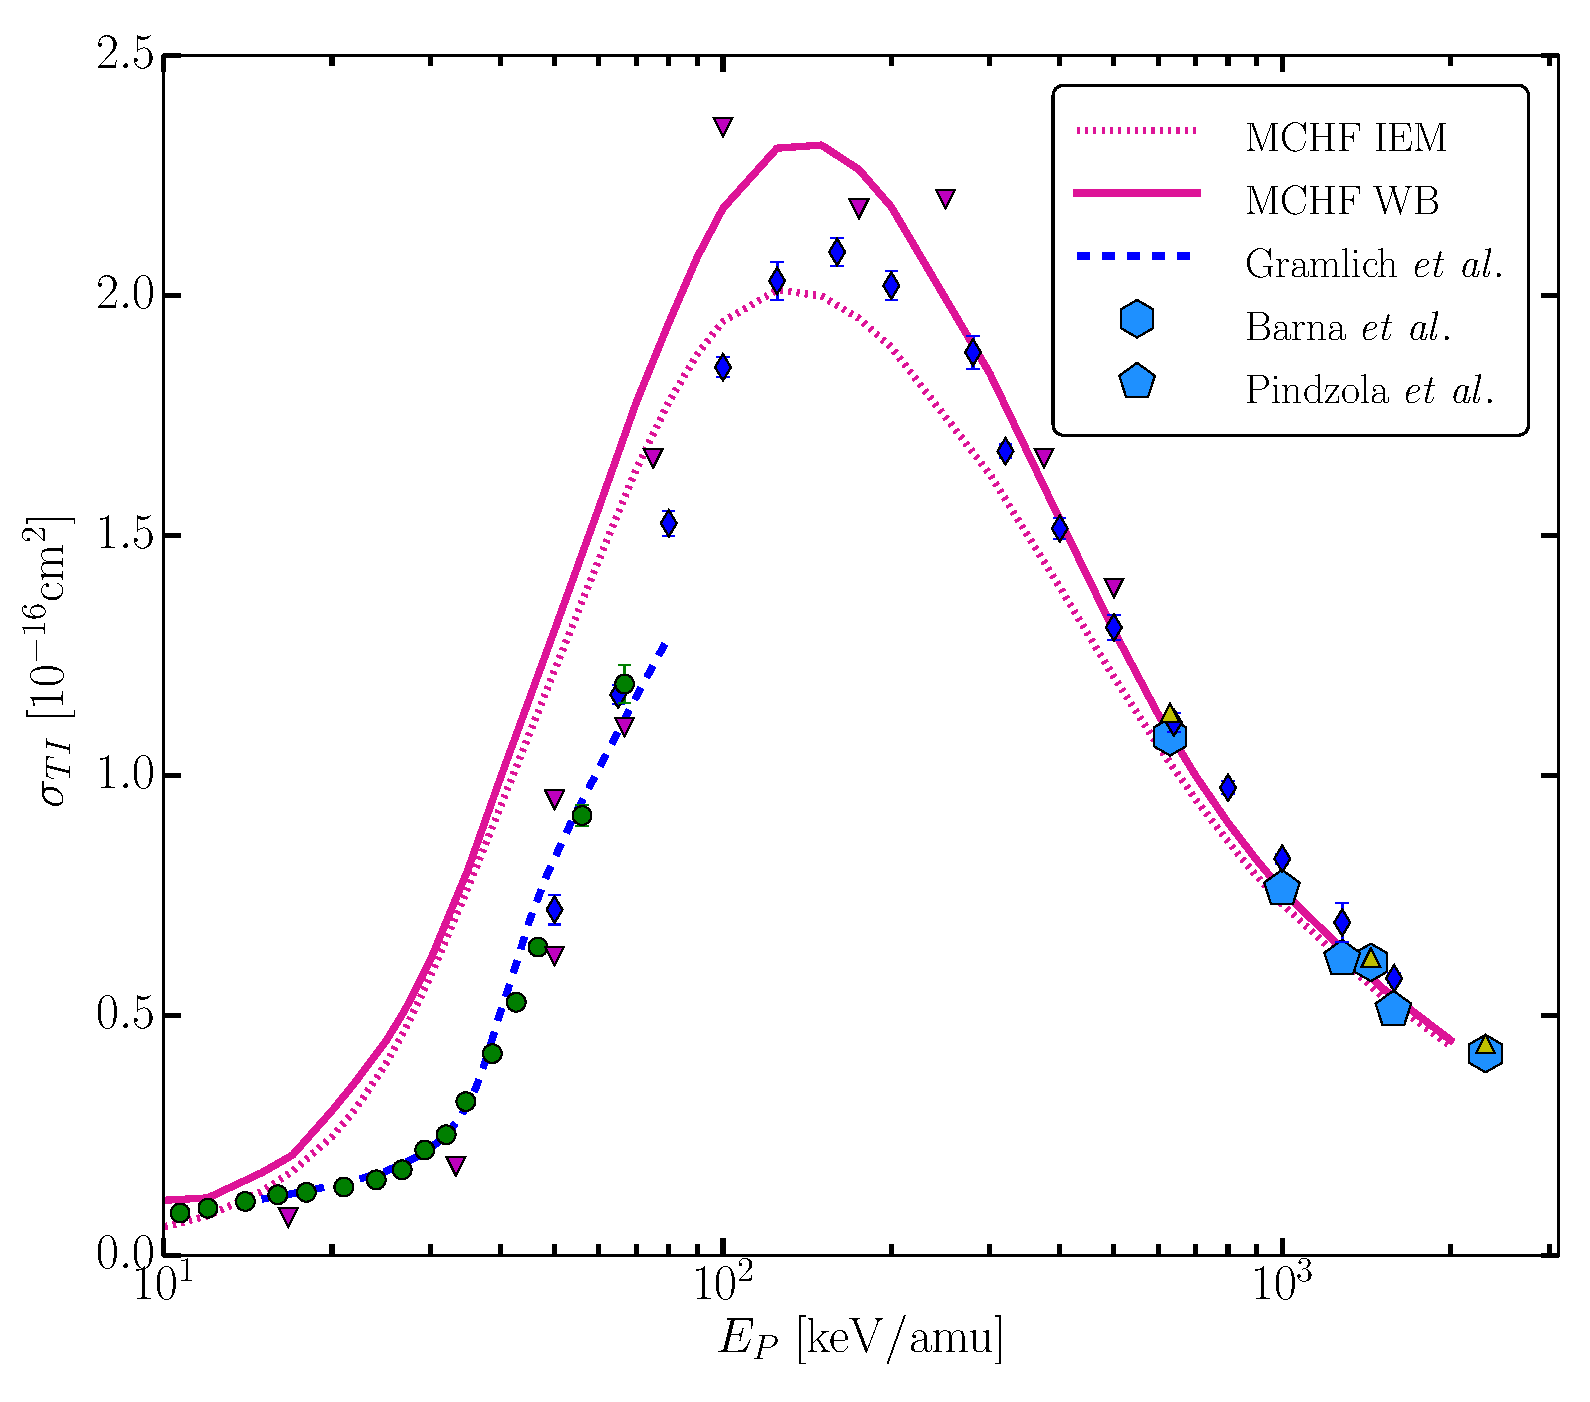
\includegraphics[width = 0.95 \linewidth]{./images/he2phe/he2phe-TI.eps}
            \caption[Total cross section for single ionization of helium by He\textsuperscript{2+}
                     impact.]{Total cross section for single ionization of helium by
                     He\textsuperscript{2+} impact. Theoretical results: Gramlich
                     et al.~\cite{GGS-89}, Barna
                     et al.~\cite{BTB-05}, and Pindzola et al.~\cite{PRC-07}.
                     Experimental data: {\color{blue}{$\blacklozenge$}}~\cite{SG85},
                     {\color{OliveGreen}{$\bullet$}}~\cite{SG89},
                     {\color{RedViolet}{$\blacktriangledown$}}~\cite{Dubois87}, and
                     {\color{GreenYellow}$\blacktriangle$}~\cite{KAH84}. \label{fig:he2phe-ti}}
         \end{figure}

         \begin{figure}[t]
            \centering
            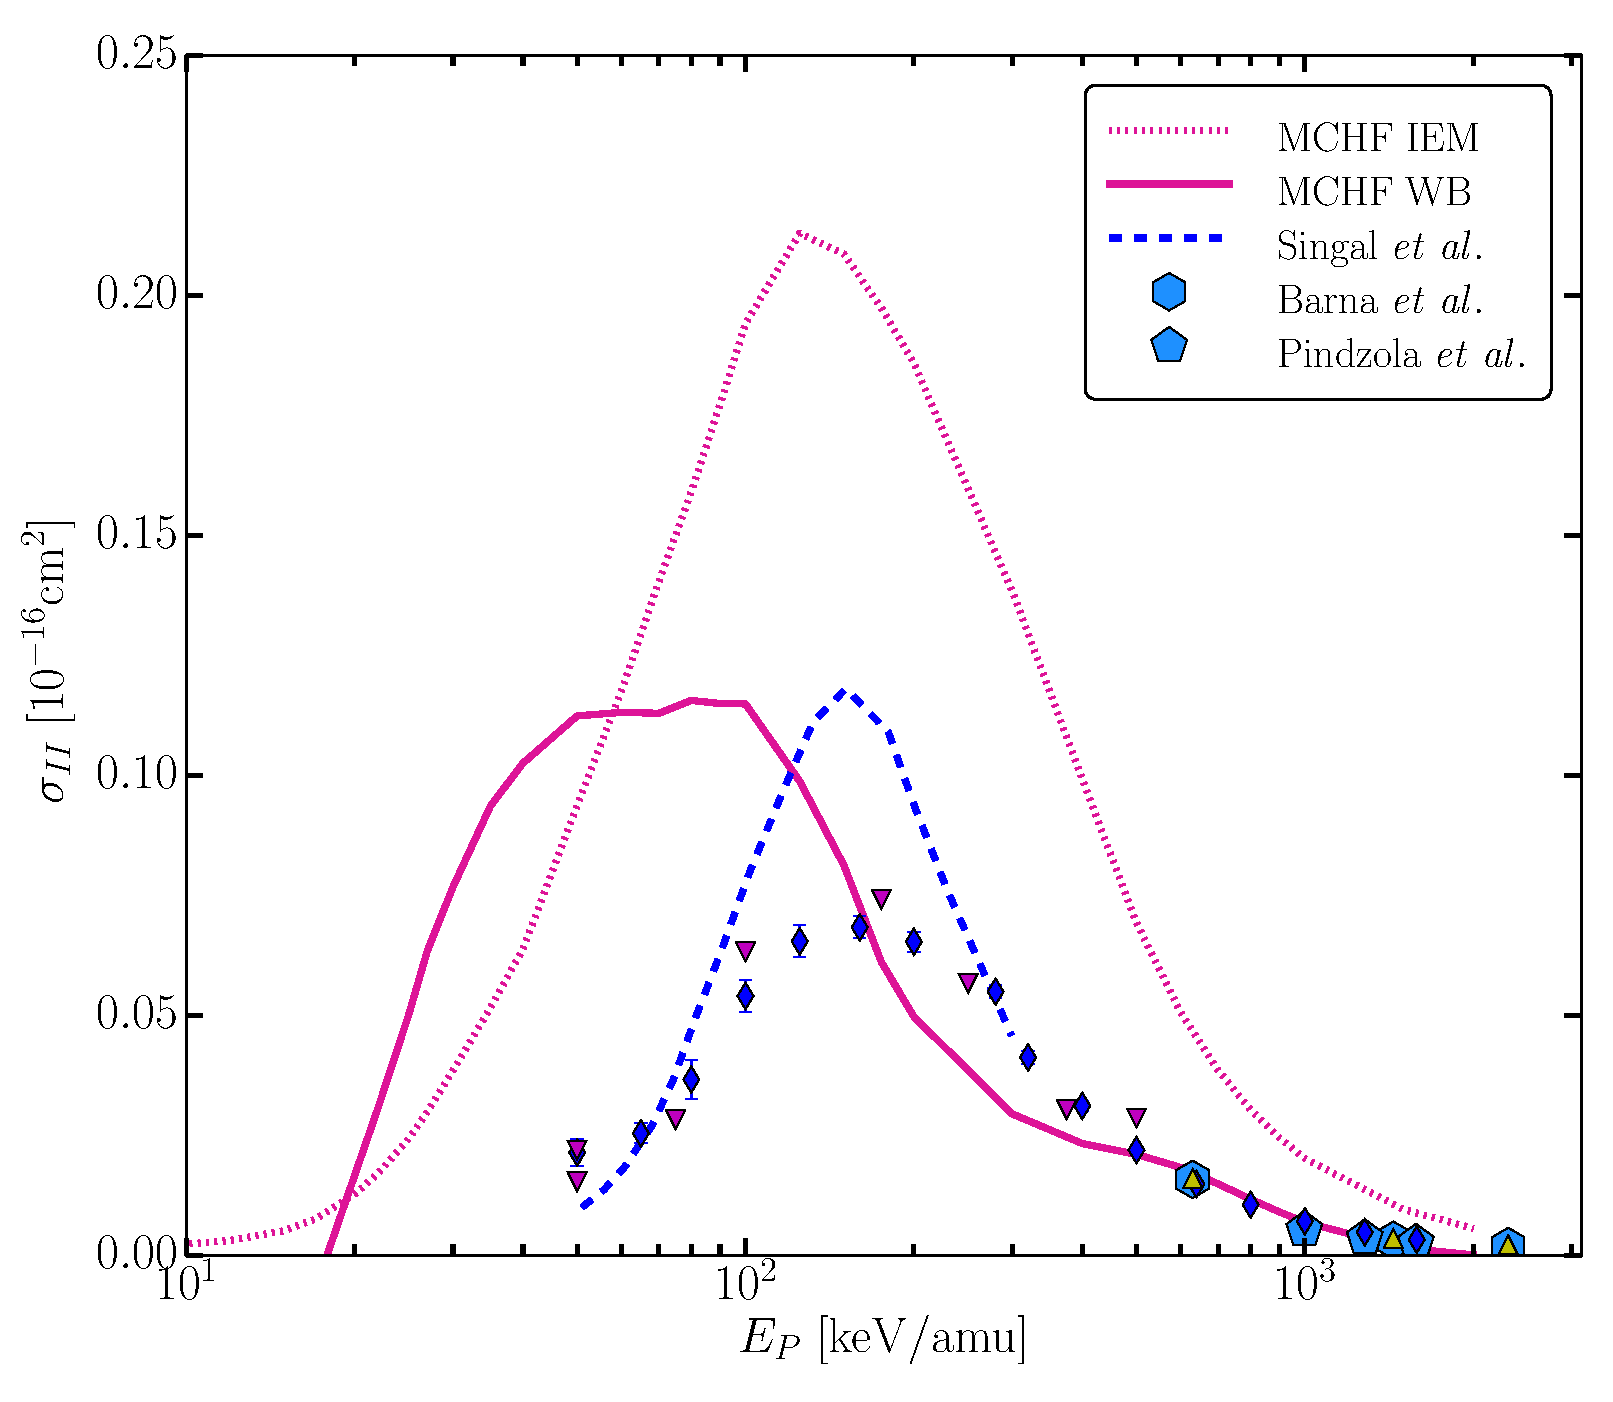
\includegraphics[width = 0.95 \linewidth]{./images/he2phe/he2phe-II.eps}
            \caption[Total cross section for double ionization of helium by He\textsuperscript{2+}
                     impact.]{Total cross section for double ionization of helium by
                     He\textsuperscript{2+} impact. Theoretical results: Singal
                     et al.~\cite{SL-91}, Barna
                     et al.~\cite{BTB-05}, and Pindzola et al.~\cite{PRC-07}
                     Experimental data: {\color{blue}{$\blacklozenge$}}~\cite{SG85},
                     {\color{RedViolet}{$\blacktriangledown$}}~\cite{Dubois87}, and
                     {\color{GreenYellow}$\blacktriangle$}~\cite{KAH84}. \label{fig:he2phe-ii}}
         \end{figure}

         \begin{figure}[t]
            \centering
            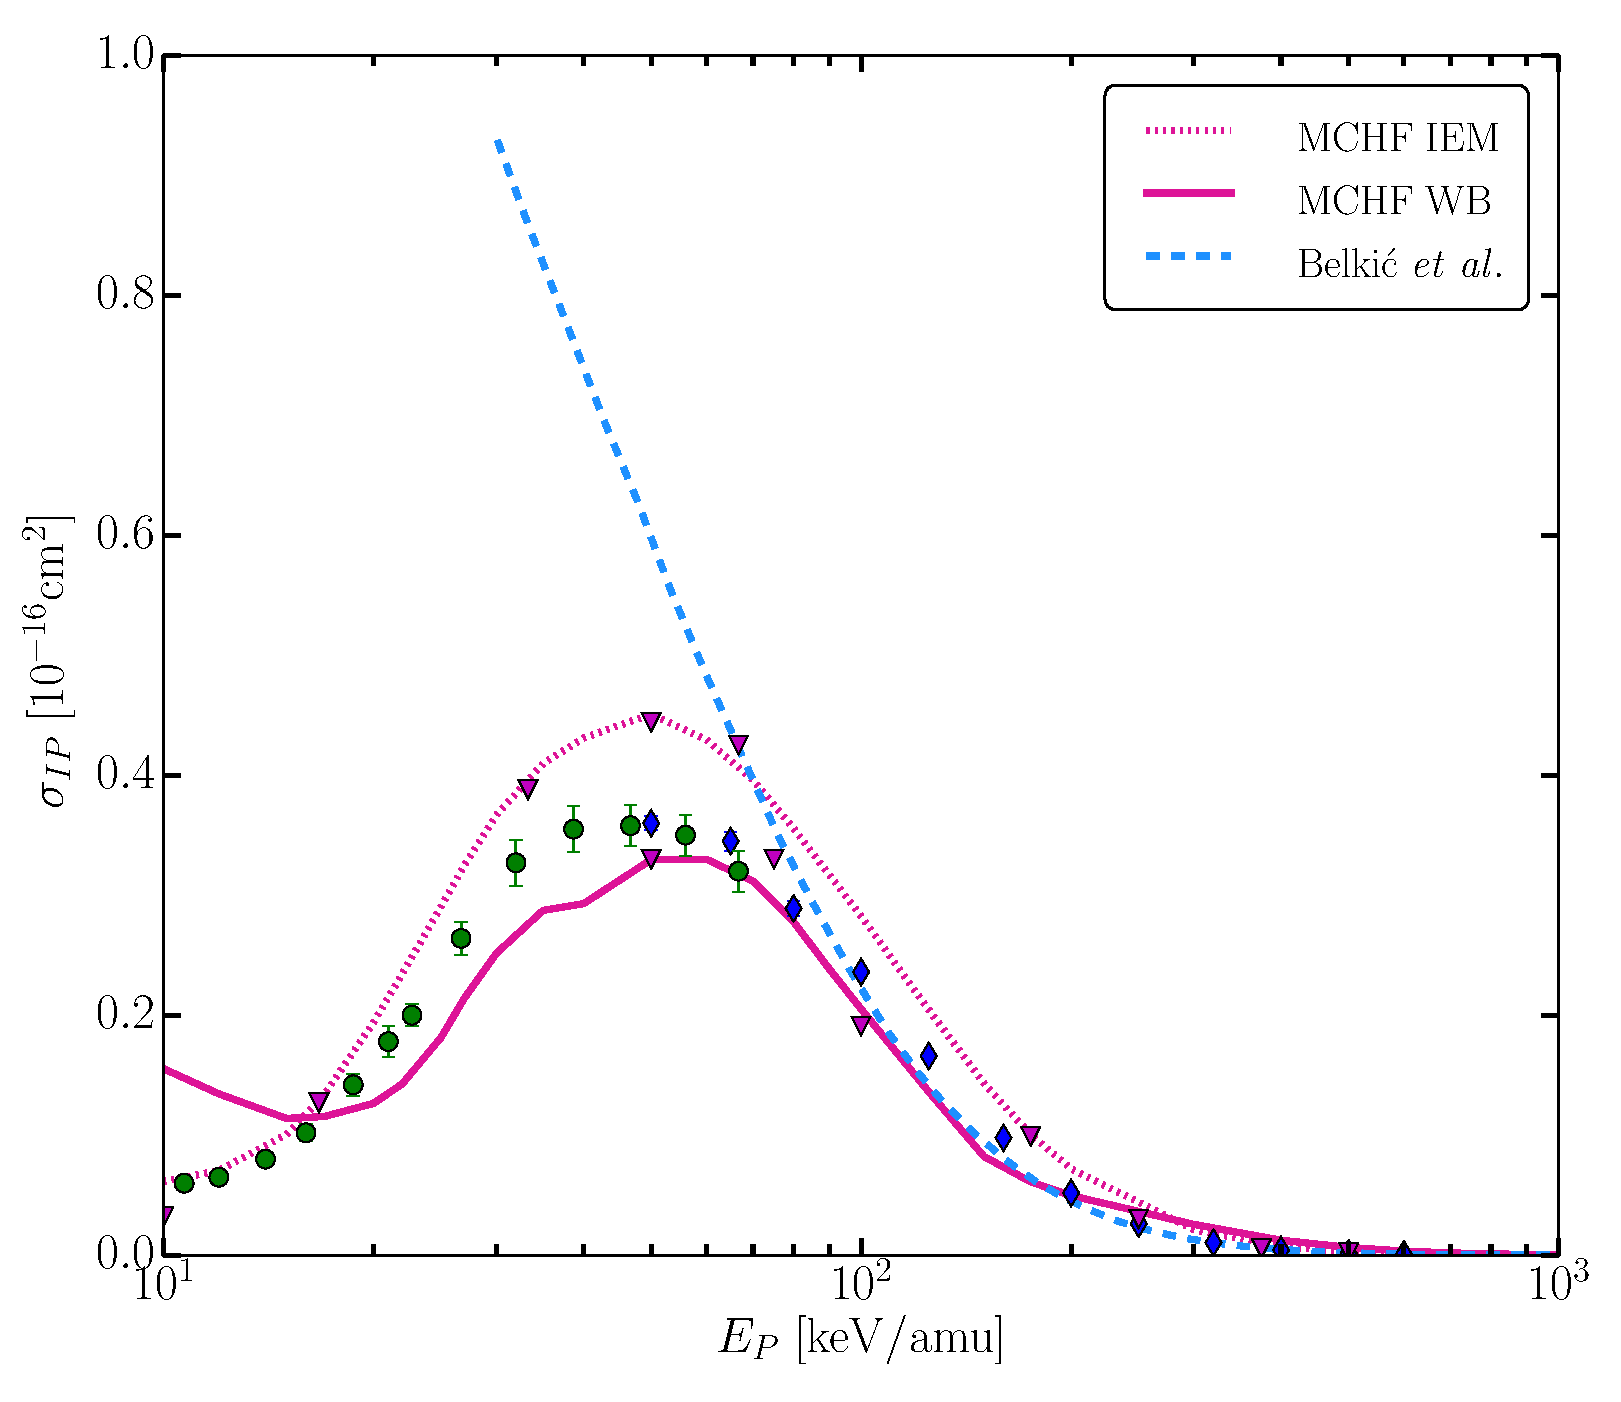
\includegraphics[width = 0.95 \linewidth]{./images/he2phe/he2phe-IP.eps}
            \caption[Total cross section for transfer ionization in He\textsuperscript{2+}-He
                     Collisions.]{Total cross section for transfer ionization in
                     He\textsuperscript{2+}-He Collisions. Theoretical results: Belki\'{c}
                     et al.~\cite{BMM-97}.
                     Experimental data: {\color{blue}{$\blacklozenge$}}~\cite{SG85},
                     {\color{OliveGreen}{$\bullet$}}~\cite{SG89}, and
                     {\color{RedViolet}{$\blacktriangledown$}}~\cite{Dubois87}. \label{fig:he2phe-ip}}
         \end{figure}

         \begin{figure}[t]
            \centering
            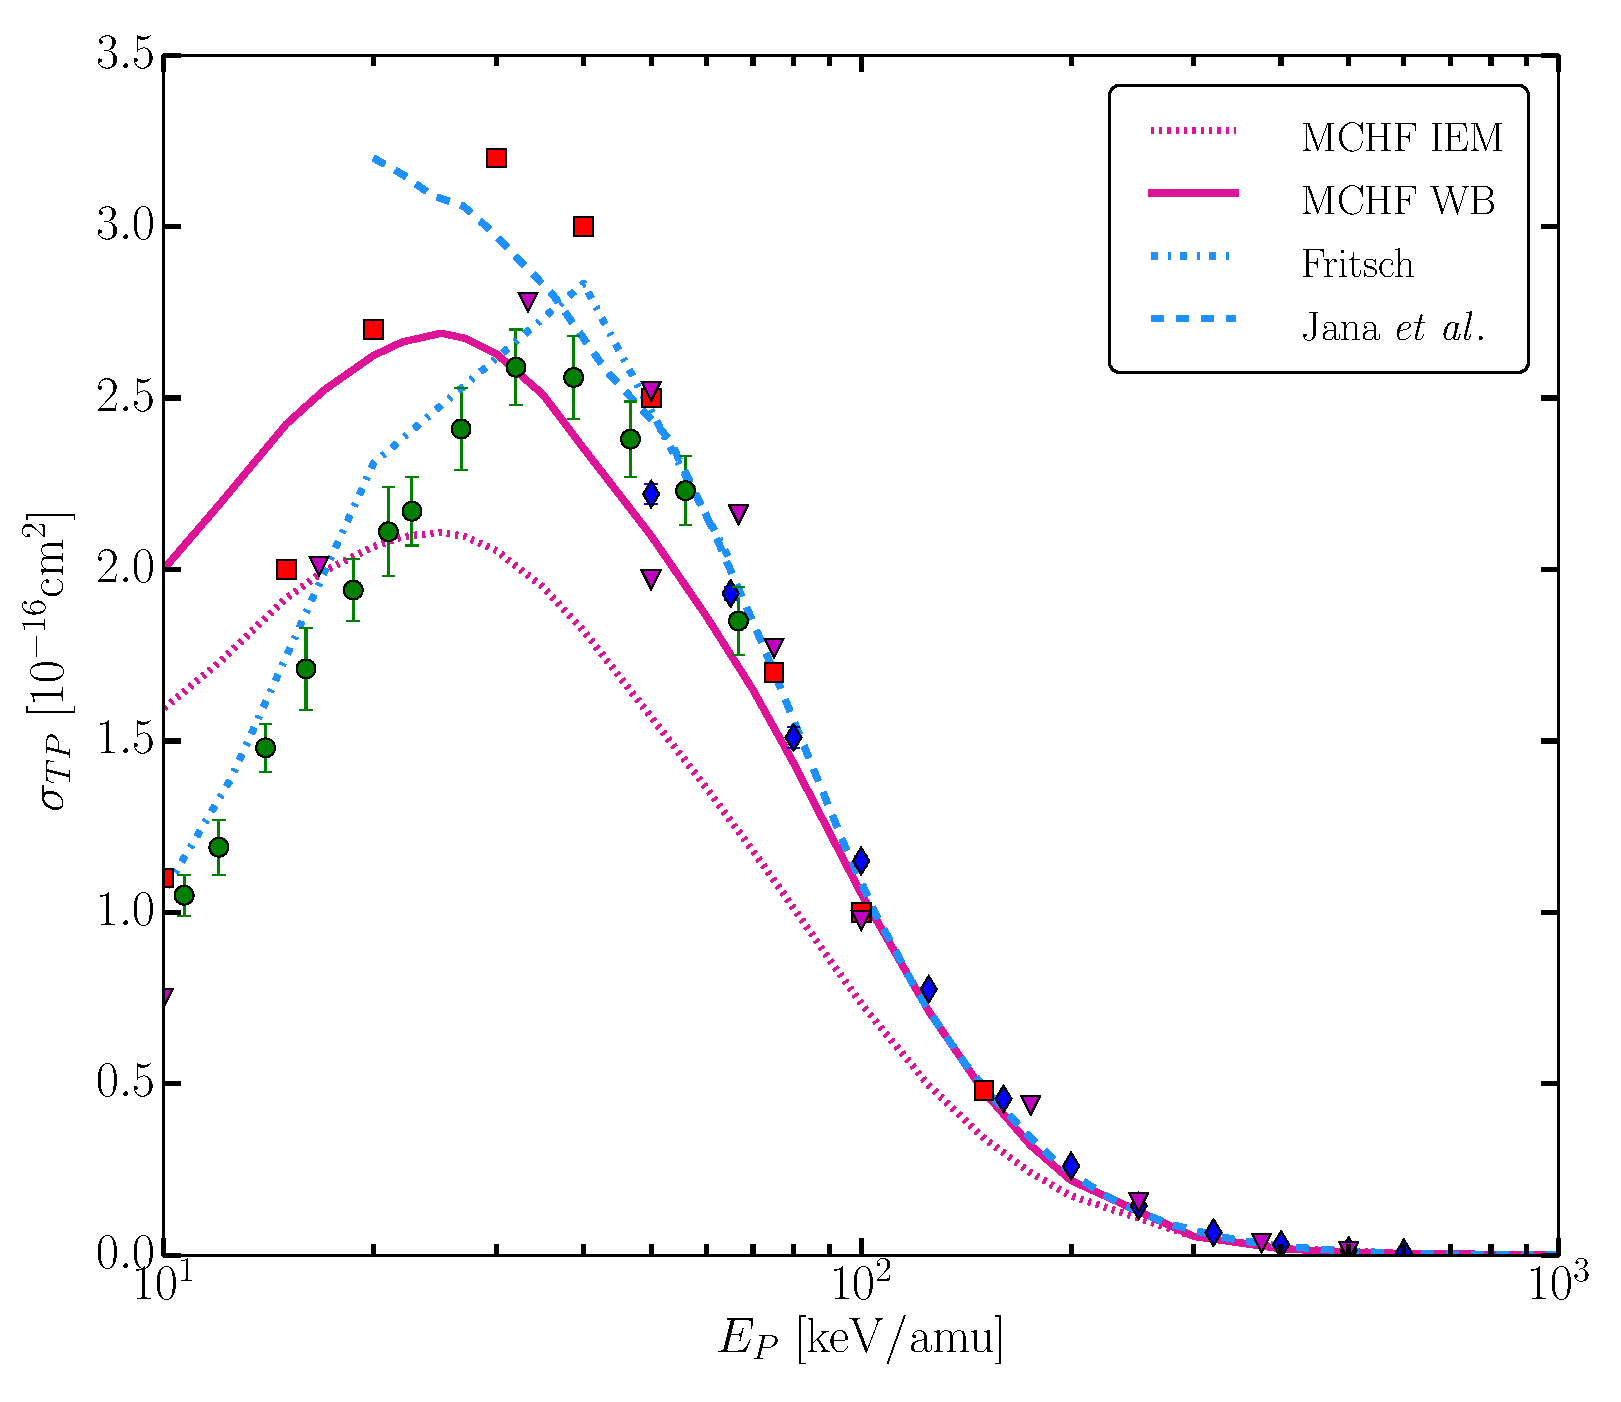
\includegraphics[width = 0.95 \linewidth]{./images/he2phe/he2phe-TP.eps}
            \caption[Total cross section for single capture in He\textsuperscript{2+}-He
                     collisions.]{Total cross section for single capture in He\textsuperscript{2+}-He
                     collisions. Theoretical results: Fritsch~\cite{Fritsch-94} and \textsc{dw-4b} of
                     Jana et al.~\cite{JMP-15}.
                     Experimental data: {\color{blue}{$\blacklozenge$}}~\cite{SG85},
                     {\color{OliveGreen}{$\bullet$}}~\cite{SG89},
                     {\color{RedViolet}{$\blacktriangledown$}}~\cite{Dubois87}, and
                     {\color{red}$\blacksquare$}~\cite{Rudd85}. \label{fig:he2phe-tp}}
         \end{figure}

         \begin{figure}[h]
            \centering
            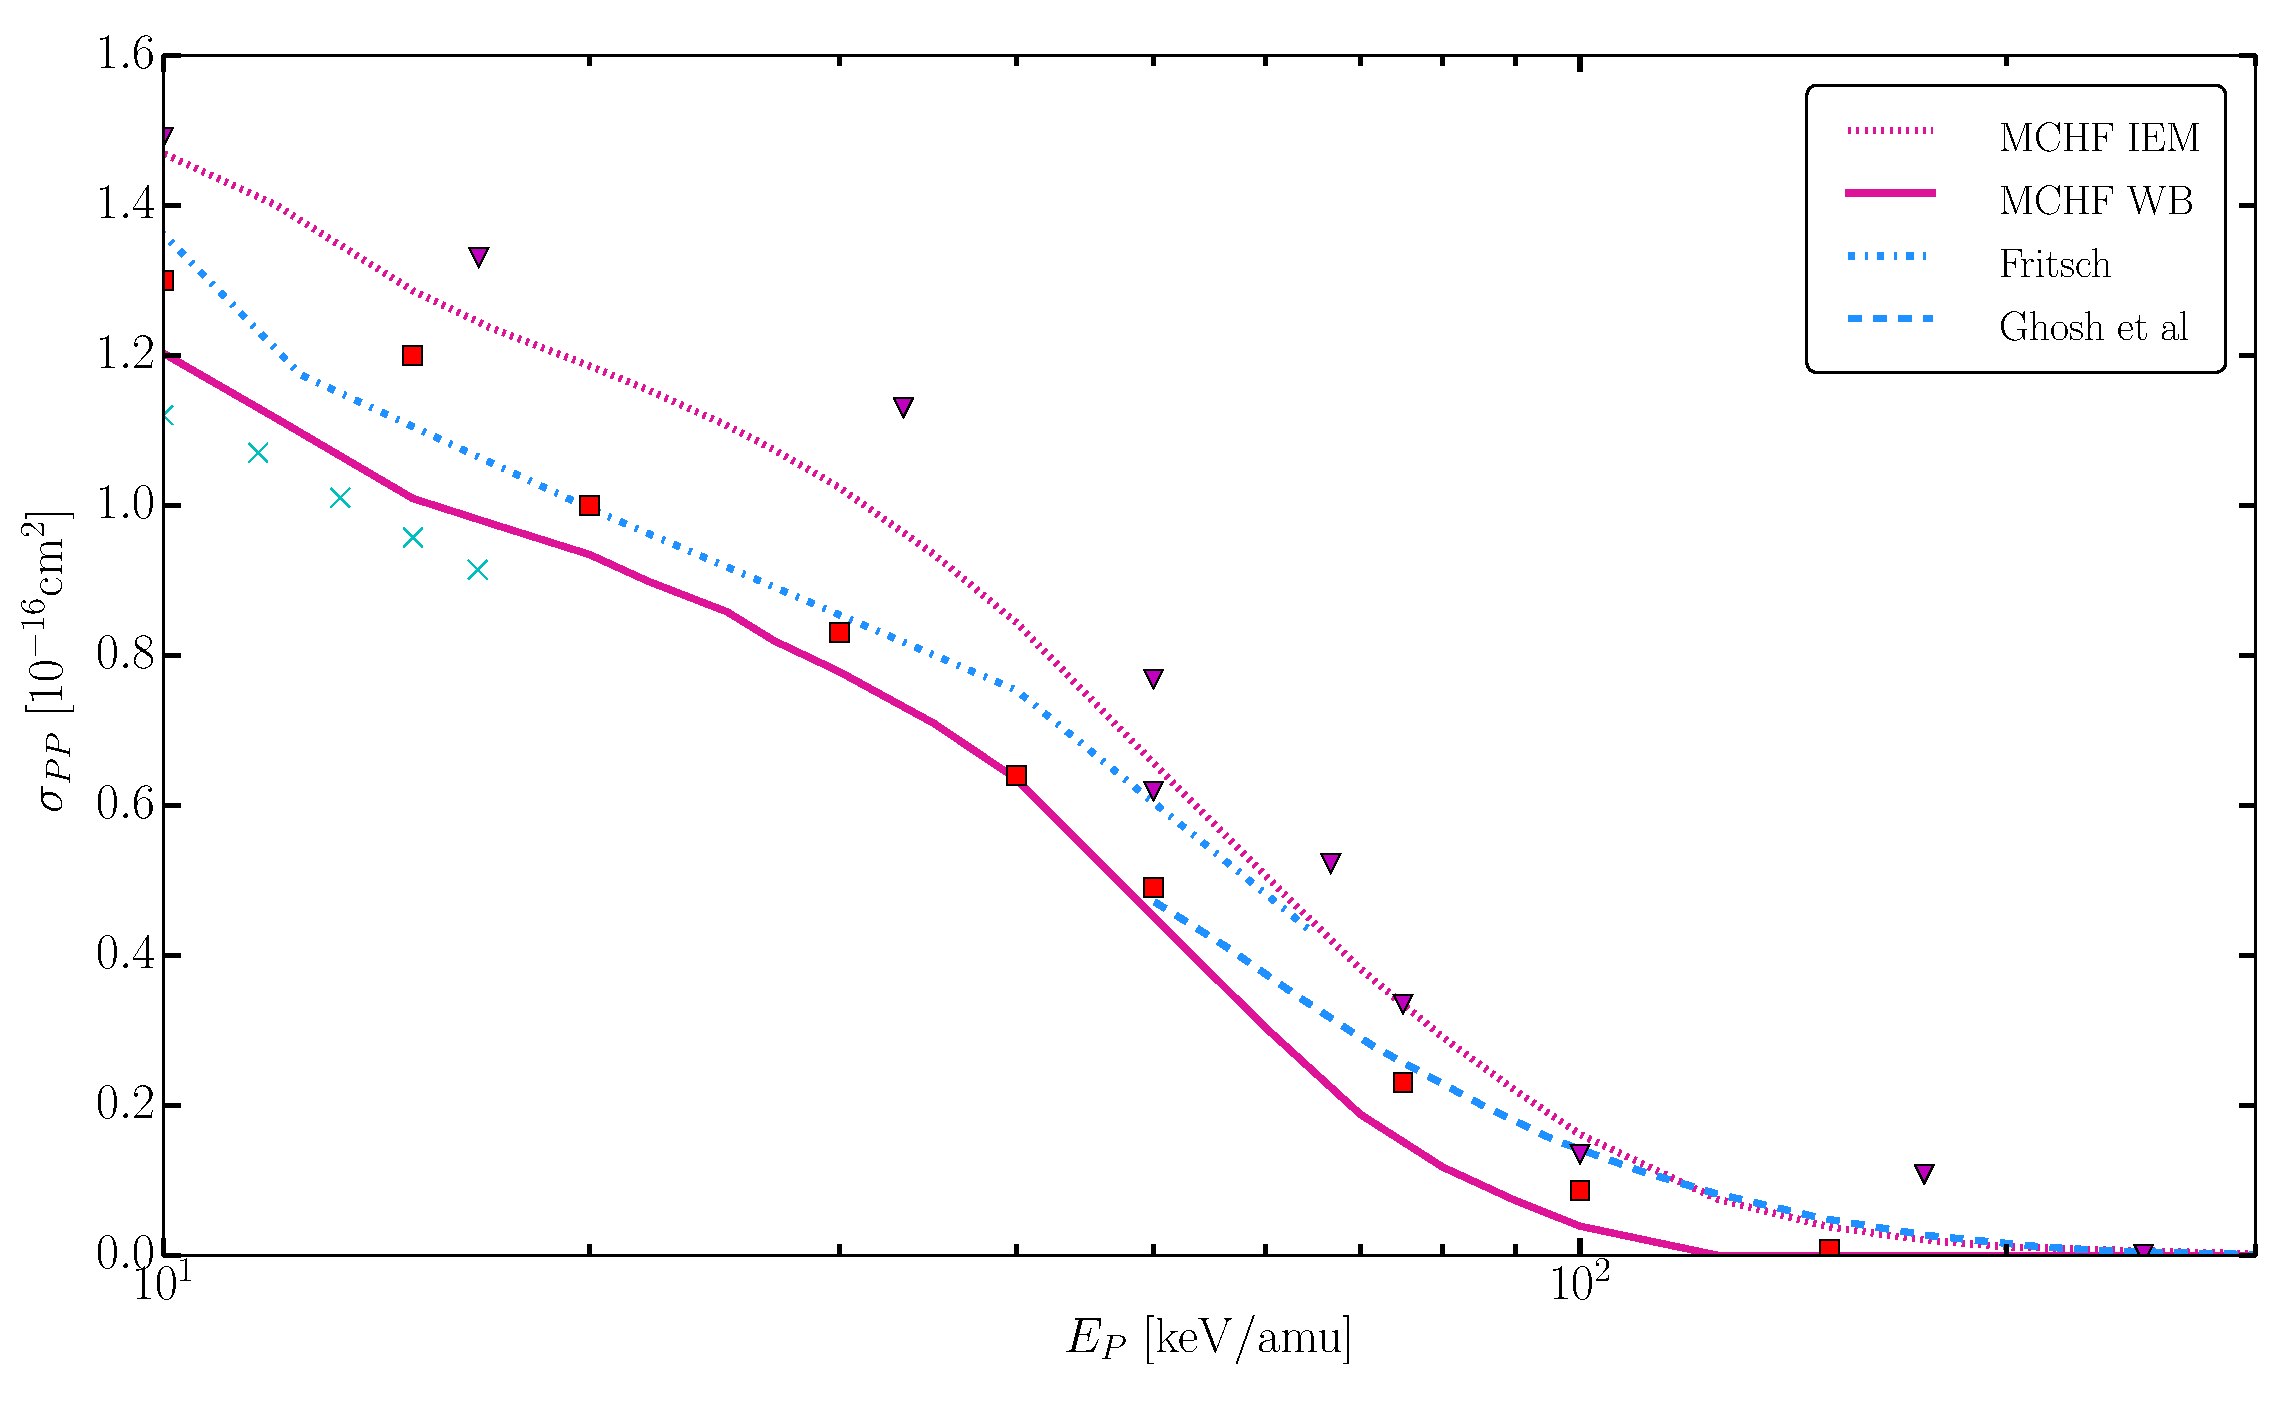
\includegraphics[width = 0.95 \linewidth]{./images/he2phe/he2phe-PP.eps}
            \caption[Total cross section for double capture in He\textsuperscript{2+}-He
                     collisions.]{Total cross section for double capture in He\textsuperscript{2+}-He
                     collisions.
                     Theoretical results: Fritsch~\cite{Fritsch-94} and Ghosh
                     et al.~\cite{GDMP-08}.
                     Experimental data: {\color{RedViolet}{$\blacktriangledown$}}~\cite{Dubois87},
                     {\color{red}$\blacksquare$}~\cite{Rudd85}, and
                     {\color{TealBlue}$\times$}~\cite{SG74}. \label{fig:he2phe-pp}}
         \end{figure}

         The results of the He\textsuperscript{2+}-He calculations for both \textsc{iem} and \textsc{wb}
         model and experimental data are presented in Figs.~\ref{fig:he2phe-ti}--\ref{fig:he2phe-pp}
         along with an assortment of previous, correlated theoretical calculations. As with our
         proton-helium results single ionization (Fig.~\ref{fig:phe-ti}) in both the \textsc{iem} and
         \textsc{wb} model are quite similar excluding an energy range around the maximum where the
         \textsc{wb} increases the cross section significantly. In both cases the peak appears to be
         shifted to a slightly lower impact energy compared to the measurements. Similar behaviour below
         100~keV/amu see the pair falling above experiment. Depicted along side the current results in
         Fig.~\ref{fig:he2phe-ti} are the previous calculations of Gramlich et al.~\cite{GGS-89}, Barna
         et al.~\cite{BTB-05}, and Pindzola et al.~\cite{PRC-07}. At the high end of the energy range
         explored all results are in agreement. At lower energies (approximately 15--80~keV/amu) the
         results of Gramlich et al.\ are in much better agreement with experiment. This region is
         precisely the range where capture is dominant and quite strong. As a result $p_T < 1/2$ for a
         significant portion of this range causing $I^{TT}_\mathrm{c} = -{p_T}^2$. A negative
         $I^{TT}_\mathrm{c}$ will increase $p^{TI}$, luckily $I^{TP}_\mathrm{c}$ is enough to keep the
         \textsc{wb} results from exceeding those of the \textsc{iem}  [cf.\ Eq.~\eqref{eq:pti-ic}]. The
         lack of correlated calculations near the experimental maximum unfortunately means little can be
         concluded in this region of the curve.

         The \textsc{wb} results for double ionization, Fig.~\ref{fig:he2phe-ii}, display the familiar
         pattern seen in both antiproton and proton collisions, namely, fair agreement with experiment
         at high impact energies coupled with overestimation of the data at lower energies and a
         reduction over \textsc{iem}. It should be noted that due to the size of the error bars of the
         low energy $\bar{p}$-He data what constitutes an overestimation is difficult to determine
         (\textsc{wb} results do tend towards the upper limits of these error bars). It would seem that
         such behaviour is a general feature of the \textsc{wb} model. For the positively-charged
         projectiles the \textsc{wb} model causes a shift in the maximum to lower energies. Much like
         the $p$-He results there are slight fluctuations in the He\textsuperscript{2+}-He \textsc{wb}
         results due to instabilities in the dynamics.

         As above Barna et al.\ and Pindzola et al.\ support the high energy \textsc{wb}
         results. Fig.~\ref{fig:he2phe-ii} also includes the results of Singal et al., while
         not a two-electron calculation it incorporates a modified single-particle potential designed to
         account for the increased difficulty of ionizing two electrons. If nothing else these results
         confirm the placement of the position of the \textsc{iem} cross section maximum. This confirms
         the belief that the \textsc{wb} model becomes less dependable at lower energies.

         Unlike for the proton-helium system double ionization and transfer ionization,
         Fig.~\ref{fig:he2phe-ip}, are not identical. The increased role of capture due to the deeper
         potential well of the He\textsuperscript{2+} projectile has the important consequence of
         allowing the $p_P$ to rise above the critical one half threshold. As a result
         $I^{PP}_\mathrm{c}$ is no longer trivial, and the bounds defining $I^{TP}_\mathrm{c}$ vary more
         freely. The \textsc{wb} model reduces \textsc{iem} results through most of the impact energy
         range. A slight over-reduction occurs to the left of the peak. Below 20~keV/amu the results
         begin to swing drastically upwards to compensate for the fact that double ionization becomes
         zero in this region. As mentioned above the ripples present in the \textsc{wb} curve are due to
         instabilities in the dynamics.

         Much like the $p$-He system few calculations exist beyond the level of the \textsc{iem} for the
         transfer ionization channel. Presented is the post form of the four-body continuum
         distorted-wave  approximation results of Belki\'{c} et al.~\cite{BMM-97}. As mentioned above
         the post form includes explicit dynamic correlation. At the extremes of the energy range
         Belki\'{c} et al. are in better agreement with experiment, as the \textsc{wb} and \textsc{iem}
         slightly exaggerate the cross section (similar to the $p$-He results). These discrepancies
         become larger as the peak is approached from above. It is difficult to ascertain how much of
         this widening gap between our \textsc{wb} results and Belki\'{c} et al.'s calculation is a
         result of the increased importance of dynamic correlation. Certainly this is the primary
         difference down to 80~keV/amu, below which point the perturbative calculation appears to break
         down making it of less utility for the current purpose.

         Single capture cross sections, presented in Fig.~\ref{fig:he2phe-tp}, also follow a pattern
         similar to that laid out by the proton-helium case: an increase in the \textsc{wb} over
         \textsc{iem}. This increase results in good agreement with experiment above 50~keV/amu. Unlike
         previous results the enhancement in cross section persists to low energies, where the
         \textsc{wb} model overestimates the measurements.

         In the high energy region of the curve the \textsc{wb} model is in fair agreement with the
         \textsc{dw-4b} results of Jana et al. It would appear the effects of dynamic correlation may
         account for the slight underestimation of the \textsc{wb} model to the right of the maximum.
         Below the peak the coupled channel results of Fritsch~\cite{Fritsch-94} lend credence to the
         experimental data. The failure of both the \textsc{wb} and \textsc{iem} models to agree with
         these results (and by extension experiment) may point to a possible failure of the underlying
         dynamic calculation in separating the target, projectile and ionizing regions ($T$, $P$ and
         $I$).

         As mentioned above the expanded role of capture causes the correlation integral
         $I^{PP}_\mathrm{c}$ to no longer be trivial. This also means that double capture in the
         \textsc{wb} model is no longer identically zero. Results for double capture are presented in
         Fig.~\ref{fig:he2phe-pp}. While the \textsc{wb} decreases the cross section below \textsc{iem}
         it is difficult to conclude whether this is an improvement due to the relatively wide spread in
         the experimental data.

         To aid in this determination we compare our results to those of Fritsch~\cite{Fritsch-94} and
         the post form of the four-body boundary corrected continuum intermediate state approximation
         (\textsc{bccis-4b}) results of Ghosh et al.~\cite{GDMP-08}. For the highest energies presented
         Ghosh et al.\ support the results of the \textsc{iem} over those of the \textsc{wb} model. In
         this region the same factors that force the $p$-He \textsc{wb} double capture channel to be
         identically zero force cross sections above 125~keV/amu into triviality. Below this limit Ghosh
         et al.\ begin to fall more in line with the \textsc{wb} results. As the results of Fritsch
         enter the picture in the lower portion of the energy range the \textsc{wb} model appears to be
         favoured, the gap between Fritsch and the \textsc{wb} being less than that between \textsc{iem}
         and Fritsch. The remaining discrepancy may be due once again to dynamic correlation effects.

      \end{subsection}

   \end{section}

\end{chapter}

\begin{chapter}{\texorpdfstring{He\textsuperscript{+}}{He+}-He Collisions \label{chap:hephe}}

   The investigations of the previous chapter began with the simplest possible multi-electron collision
   system, one where a negatively-charged projectile is incident on helium. The situation was then
   complicated by allowing the projectile to be positive, thus forcing one to consider electron transfer
   in addition to ionization processes.

   In this chapter the system of interest is expanded further by the inclusion of an active electron on
   the projectile. More specifically, the remainder of this work concerns itself with the
   He\textsuperscript{+}-He collision system.

   While the external potential, $v_\mathrm{ext}$, maintains the form of Eq.~\eqref{eq:phe2p-ext}, the
   spin-polarized nature of the collision system suggests that the spin-free description utilized in the
   previous chapter should be replaced by the full spin-dependent \textsc{tdks} presented in
   Eq.~\eqref{eq:tdks}.

   The determination of a spin-dependent exchange-correlation potential forms the bulk of this chapter
   (Sec.~\ref{sec:pot}) in which a procedure for calculating an accurate exchange potential within the
   x-only approximation is discussed. This is followed by a brief discussion of the method used to
   extract cross sections from the one-particle density (Sec.~\ref{sec:hephe-det}) before presenting
   results in Sec.~\ref{sec:hephe-disc}.

   \begin{section}{Calculating the x-Potential \label{sec:pot}}

      While the correlation potential in Eq.~\ref{eq:tdks} may be ignored, that is the x-only
      approximation may be used (with some understanding of the consequences), an accurate exchange
      potential is essential for a precise description of the He\textsuperscript{+}-He collision
      system. The spin-polarized nature of the system, which emphasizes exchange effects, makes this
      fact indisputable. To this end the \textsc{kli} approximation to the \textsc{opm}
      (see Sec.~\ref{sec:kli}) was employed in the calculation of $v^\sigma_\mathrm{x}$.

      The ground-state density functional theory scheme of~\cite{diamol}\footnote{The details of this
      implementation may be found in~\cite{diamol} and were provided by the authors via private
      communication.} has been adapted to calculate a time-dependent exchange potential. At any instant
      of time, $t$, the He\textsuperscript{+}-He system may be regarded as a diatomic quasi-molecule with
      an internuclear distance $R(t) = \sqrt{b^2 + Z(t)^2}$, where $b$ and $Z$ are the impact parameter
      and the $z$ position of the projectile as described below Eq.~\eqref{eq:phe2p-ext}. If at each
      time-step of the propagation the time-dependent Kohn-Sham orbitals,
      $\varphi_{\sigma j}(\mathbf{r},t)$ are fed into the \textsc{kli} functional (ignoring self
      consistency) an exchange potential, $v^{\sigma}_\mathrm{x}[ \{ \varphi_{\sigma^\prime j} \};t]$,
      is obtained\footnote{The normalization of the \textsc{kli} potential is chosen so that
      $v_\mathrm{x}^\textsc{kli}(\mathbf{r},t) \xrightarrow{\vert \mathbf{r} \vert \to \infty} 0$.}. In
      Ref.~\cite{diamol} the \textsc{kli} scheme has been implemented for eigenstates of a total
      \textsc{ks} potential which is invariant against rotation around the internuclear axis. This
      restriction complicates the use of the corresponding \textsc{kli} potential, since the present
      $\varphi_{j \sigma}$ do not exhibit any specific symmetry.

      In order to detail a solution to the symmetry problem a more thorough description of the
      \textsc{tc-bgm}~\cite{tcbgm} is necessary. Within the \textsc{tc-bgm} the Kohn-Sham (\textsc{ks})
      orbitals are represented in a non-orthogonal basis
      %
      \begin{equation} \label{eq:bgmexp}
         \varphi_{\sigma j}(\mathbf{r},t) = \sum\limits_{c \in \{P, T\}} \sum\limits_{k, L, M}
                               d_{c k L}^{\sigma j}(t) \tilde{\chi}^{LM}_{c k}(\mathbf{r},t),
      \end{equation}
      %
      where
      %
      \begin{equation} \label{eq:etfbasis}
         \tilde{\chi}^{L M}_{ck}(\mathbf{r},t) =
            \begin{cases}
               e^{i \mathbf{v}_T \cdot \mathbf{r}} {\chi}^{L M}_{c k}(\mathbf{r},t) & c = T, \\[2ex]
               e^{i \mathbf{v}_P \cdot \mathbf{r}} {\chi}^{L M}_{c k}(\mathbf{r},t) & c = P,
            \end{cases}
      \end{equation}
      %
      which are the basis functions with electron translation factors (\textsc{etf}) included. The basis
      functions themselves are given by [similarly to the one-centre basis of Eq.~\eqref{eq:bgmbasis}]
      %
      \begin{equation} \label{eq:bgmbasis2}
         \chi^{LM}_{ck} (\mathbf{r},t)
         = W_P( \mathbf{r},t, \epsilon_P)^L W_T(\mathbf{r}_T,\epsilon_T)^M \chi^{00}_{ck}(\mathbf{r}),
      \end{equation}
      %
      with
      %
      \begin{equation}
         W_T(\mathbf{r}_T,\epsilon_T) = \frac{1 - e^{-\epsilon_T r_T}}{r_t},
      \end{equation}
      %
      and
      %
      \begin{equation}
         W_P (\mathbf{r},t,\epsilon_P)
         = \frac{1 - e^{-\epsilon_P|\mathbf{r} - \mathbf{R}(t)|}}{|\mathbf{r}_T - \mathbf{R}(t)|},
      \end{equation}
      %
      where $\mathbf{r}_T$ represents the position vector with respect to the target centre and we are
      working in the centre of mass frame where $\mathbf{R} = \mathbf{r}_T - \mathbf{r}_P$.

      In Eq.~\eqref{eq:bgmbasis2} the functions $\chi^{00}_{ck}$ are the bound orbitals for the target
      helium atom ($c = T$) and the projectile helium ion ($c = P$). Just like in the one-centred case
      discussed in Sec.~\ref{sec:p-he2p-he-sys} the basis is simplified by including only states
      generated from the projectile potential. The regularizer is once again set to $\epsilon_P = 1$.
      The complete basis set used may be described in terms of the maximum $L$ value included for each
      bound sub-shell, 1$s$-4$f$, indexed by $k$, in the basis. These values are listed in
      Tab.~\ref{tab:basis} and total 124 basis states.

      \begin{table}
         \centering
         \caption{Description of the \textsc{tc-bgm} basis expansion. \label{tab:basis}}
         \begin{tabular}{lcccccccccccccccccccc}
            \toprule
            state            & 1s & 2s & 2p   & 3s & 3p   & 3d      & 4s & 4p     & 4d      & 4f \\
            $k$              & 1  & 2  & 3, 4 & 5  & 6, 7 & 8{-}10  & 11 & 12, 13 & 14{-}16 & 17{-}20 \\
            $L_\mathrm{max}$ & 0  & 0  & 1    & 1  & 2    & 2       & 2  & 3      & 3       & 3 \\
            \bottomrule
         \end{tabular}
      \end{table}

      It is clear from the above description that only the basis states corresponding to s-type orbitals
      will make cylindrically symmetric contributions to the \textsc{ks}-orbitals. The simplest solution
      is to only feed the 1s contributions into the \textsc{kli} functional. While higher s-states are
      also admissible they will no longer represent the most occupied subshell meaning their inclusion
      will do little to improve the accuracy of the description of a given orbital. Leaving out
      \textsc{etf}s for the time being the orbitals will take the explicit form
      %
      \begin{equation} \label{eq:1sonly}
         \varphi_{\sigma j}^{1s}(\mathbf{r},t) = a^{\sigma j}_T(t) \chi^{00}_{T1}(\mathbf{r},t)
                                               + a^{\sigma j}_P(t) \chi^{00}_{P1}(\mathbf{r},t).
      \end{equation}
      %
      The coefficients, $a^{\sigma j}_c$, are the result of projecting the \textsc{ks}-orbitals onto the
      two-dimensional subspace spanned by the target and projectile 1s-states
      %
      \begin{equation} \label{eq:proj}
         \ket{\varphi^{1s}_{\sigma j}} = \hat{P} \ket{\varphi_{\sigma j}}
                                       = \sum\limits_{c_1, c_2 \in \{T,P\}} \tilde{S}^{-1}_{c_1 c_2}
                                                      \ket{\chi^{00}_{c_1 1}}
                                                      \braket{\chi^{00}_{c_2 1}| \varphi_{\sigma j}}
      \end{equation}
      %
      with $\tilde{S}^{-1}_{c_1 c_2}$ the inverse of the overlap matrix
      %
      \begin{equation} \label{eq:overlap2d}
         \tilde{S}_{c_1 c_2} = \braket{ \chi^{00}_{c_1 1} | \chi^{00}_{c_2 1} }.
      \end{equation}
      %
      The coefficients are then determined to be
      %
      \begin{equation} \label{eq:coef}
         a^{\sigma j}_c = \sum\limits_{c_1, c_2 \in \{T,P\}} \sum\limits_{k = 1}^K
                          \sum\limits_{l = 0}^L \tilde{S}^{-1}_{c c_1} S^{c_2 \, k \, l}_{c \, 1 \, 0}
                             d^{\sigma j}_{c_2 k l},
      \end{equation}
      %
      with
      %
      \begin{equation} \label{eq:overlap}
         S_{c_1 \, k_1 \, l_1 }^{c_2 \, k_2 \, l_2 } =
            \braket{ \chi^{l_1 0}_{c_1 k_1} | \chi^{l_2 0}_{c_2 k_2} }
      \end{equation}
      %
      the full overlap matrix.

      Returning to the question of the \textsc{etf}s, working in the rotating centre of mass frame in
      which the $z$-direction points along the internuclear axis the \textsc{etf}s become
      %
      \begin{subequations} \label{eq:etf}
         \begin{equation} \label{eq:etfT}
            e^{i \mathbf{v}_T \cdot \mathbf{r}} =
             e^{\frac{i V}{2} (x \sin \theta - z \cos \theta)},
         \end{equation}
         %
         \begin{equation} \label{eq:etfP}
            e^{i \mathbf{v}_P \cdot \mathbf{r}} =
             e^{\frac{i V}{2} (z \cos \theta - x \sin \theta)},
         \end{equation}
      \end{subequations}
      %
      where $\theta = \arctan b/Z$ and $V$ is the relative velocity of the centers, the same velocity
      appearing below Eq.~\eqref{eq:phe2p-ext}. If we now introduce a two-centred coordinate system,
      placing the foci at the two nuclear centres it becomes clear that the portion of the \textsc{etf}s
      containing $x$ violates the desired cylindrical symmetry (see Sec.~\ref{sec:prolate}).

      Two obvious solutions present themselves. First, one may simply ignore the \textsc{etf}s
      completely. This would amount to passing the orbitals described by Eq.~\eqref{eq:1sonly} into
      the \textsc{kli} functional. Alternatively the symmetry breaking portions of the \textsc{etf}s
      may be dropped. In this case the full 1s-only \textsc{ks}-orbital becomes
      %
      \begin{equation} \label{eq:1sonlyetf}
         \tilde{\varphi}_{\sigma j}^{1s} (\mathbf{r},t) =
                      a^{\sigma j}_T (t)  e^{-\frac{i V z \cos \theta}{2}} \chi^{0}_{T1} (\mathbf{r},t)
                    + a^{\sigma j}_P (t)  e^{ \frac{i V z \cos \theta}{2}} \chi^{0}_{P1} (\mathbf{r},t).
      \end{equation}
      %
      This will offer at least some of the correction provided by the full \textsc{etf}. Unfortunately,
      as the internuclear coordinate $Z(t)$ approaches zero (corresponding to $\theta = \frac{\pi}{2}$)
      the partial \textsc{etf} will tend to one, meaning that when the target and projectile are at
      their closest, the most active region of the collision, no \textsc{etf} will be present.

      Any investigation of the impact of the \textsc{etf}s is best carried out in an isolated
      environment. To achieve this we may introduce a no-response model. In such a model the initial
      occupations of the orbitals passed to the \textsc{kli} functional will be frozen and the full
      orbitals will be propagated in the resulting potential. To be more concrete, if we have two
      spin-up and one spin-down electron the coefficients be given the fixed values
      %
      \begin{equation} \label{eq:noresp}
         \tilde{a}^{\uparrow 1}_T = \tilde{a}^{\uparrow 2}_P = \tilde{a}^{\downarrow 1}_T  = 1
         ~~~ \mbox{and} ~~~
         \tilde{a}^{\uparrow 1}_P = \tilde{a}^{\uparrow 2}_T = \tilde{a}^{\downarrow 1}_P  = 0.
      \end{equation}
      %
      In this way the only phase information entering the exchange functional will arise directly from
      the \textsc{etf}s.

      Regardless of which option is chosen it is important that $v_\mathrm{H}$ be determined with the
      same set of orbitals used in the calculation of $v_\mathrm{x}^\sigma$, preserving the precise
      cancellation of the self interaction present in the Hartree potential. A description of some of
      the technical details of the process of propagating the \textsc{ks}-orbitals in these
      time-dependent potentials are provided in Appendix~\ref{chap:calcdeets}. A collection of
      visualizations of this process may be found in Sec.~\ref{sec:visual} along with several figures
      which illustrate the time evolution of the collision system.

   \end{section}

   \begin{section}{Final-state analysis \label{sec:hephe-det}}

      Of interest in any scattering problem is the probability of finding the system in some final state.
      If we represent the state being considered as $\ket{f_1 \, f_2 \, f_3}$ and the initial state of
      the system propagated to some final time $t_f$ by $\ket{\varphi_{ \uparrow 1} \,
      \varphi_{\uparrow 2} \, \varphi_{\downarrow 1} (t_f)}$ the exclusive probability to find the
      system in the given final state at time $t_f$ will be given by
      %
      \begin{equation} \label{eq:finalProb}
         P_{f_1 f_2 f_3}(t_f) = \left| \braket{ f_1 \, f_2 \, f_3 | \varphi_{ \uparrow 1} \,
                                       \varphi_{\uparrow 2} \, \varphi_{\downarrow 1} (t_f) } \right|^2.
      \end{equation}
      %
      If one assumes that both the propagated and final states can be represented as a single Slater
      determinant then the probability in question becomes
      %
      \begin{equation} \label{eq:detProb}
         P_{f_1 f_2 f_3}(t_f) = \det \left[ \gamma_{f f^\prime}(t_f) \right],
      \end{equation}
      %
      where $\gamma_{f f^\prime}$ is the one-particle density matrix
      %
      \begin{equation} \label{eq:denmat}
         \gamma_{f f^\prime}(t_f) = \sum\limits_{\sigma} \sum\limits_{j = 1}^{N_\sigma}
                               \braket{f | \varphi_{\sigma j}(t_f)}
                               \braket{\varphi_{\sigma j}(t_f) | f^\prime},
      \end{equation}
      %
      with $f$ and $f`$ $\in \{f_1, f_2, f_3\}$, and the transition amplitudes
      %
      \begin{equation}
         \braket{f | \varphi_{\sigma j}(t_f)}
         = \braket{\tilde{\chi}^{l0}_{c k} | \varphi_{\sigma j}(t_f)}
      \end{equation}
      (for some $k$, $l$, $c$, and properly orthogonalized basis functions $\tilde{\chi}^{l0}_{c k}$)
      readily calculable from the dynamics. A model of this type which ignores the functional
      correlations discussed in Sec.~\ref{sec:phe2p-obs} is consistent with an \textsc{iem} description,
      An example of such a description is provided in Appendix~\ref{chap:moreIc} (in particular
      Eq.~\eqref{eq:iem3}). Expressions similiar to Eq.~\eqref{eq:prob-iem} may be constructed in this
      context. The key to the derivation comes from expressing the single-particle probabilities in
      terms of the transition amplitudes, for example, $p_T$ may be written
      %
      \begin{equation} \label{eq:ptTrans}
         p_T = \frac{1}{3} \sum\limits_{\sigma} \sum\limits_{j = 1}^{N_\sigma} \sum\limits_{k = 1}^{K}
               \left| \braket{ \tilde{\chi}^{00}_{T k} | \varphi_{\sigma j}(t_f)}\right|^2,
      \end{equation}
      %
      with $p_P$ and $p_I$ expressed similarly.

      Alternatively, one could consider the probability to explicitly measure the states of some subset
      of the total number of particles. These so called inclusive probabilities can be expressed in
      terms of determinants of submatrices of the density matrix~\cite{inc-prob}.

      In the current problem we are interested in those probabilities which correspond to the possible
      outcome channels of in the He\textsuperscript{+}-He collision system. The processes can be broadly
      categorized into those that involve one active electron:
      %
      \begin{equation} \label{eq:tpi111}
         \mathrm{He}^+ + \mathrm{He} \rightarrow \mathrm{He}^+ + \mathrm{He}^+ + e^-
      \end{equation}
      %
      \begin{equation} \label{eq:tpi120}
         \mathrm{He}^+ + \mathrm{He} \rightarrow \mathrm{He} + \mathrm{He}^+
      \end{equation}
      %
      \begin{equation} \label{eq:tpi201}
         \mathrm{He}^+ + \mathrm{He} \rightarrow \mathrm{He}^{2+} + \mathrm{He} + e^-,
      \end{equation}
      %
      two active electrons:
      %
      \begin{equation} \label{eq:tpi012}
         \mathrm{He}^+ + \mathrm{He} \rightarrow \mathrm{He}^+ + \mathrm{He}^{2+} + 2e^-
      \end{equation}
      %
      \begin{equation} \label{eq:tpi102}
         \mathrm{He}^+ + \mathrm{He} \rightarrow \mathrm{He}^{2+} + \mathrm{He}^+ + 2e^-
      \end{equation}
      %
      \begin{equation} \label{eq:tpi021}
         \mathrm{He}^+ + \mathrm{He} \rightarrow \mathrm{He} + \mathrm{He}^{2+} + e^-,
      \end{equation}
      %
      and three active electrons:
      \begin{equation} \label{eq:tpi003}
         \mathrm{He}^+ + \mathrm{He} \rightarrow \mathrm{He}^{2+} + \mathrm{He}^{2+} + 3e^{-}.
      \end{equation}
      %
      Additionally there is the channel where no charges are transferred and the two channels that result
      in the production of He\textsuperscript{-}. Cross sections for the latter are known to be
      negligible~\cite{metahe, neghe-neg}.

      In such configurations we find $k$ particles on the projectile, $l$ particles in the continuum,
      and $3 - k - l$ on the target ($0\leq k \leq 3$ and $0 \leq l \leq 3 - k$). The probabilities
      $p_{kl}$ may be calculated in terms of sums of inclusive probabilities to find a given number of
      particles in the bound states of the target and projectile by applying the machinery
      of~\cite{inc-prob} (see for example~\cite{incEx, mitsuko12, gerald15}). The probabilities of
      interest take the form
      %
      \begin{equation} \label{eq:probGer1}
         P^\prime_{kl} = \sum\limits_{\substack{f_1 < \dots < f_k \\ f \in \mathcal{P}}}
                         \sum\limits_{\substack{f_{k+1} < \dots < f_{k+l} \\ f \in \mathcal{I}}}
                         P_{f_1 \dots f_{f_{k+l}}},
      \end{equation}
      %
      then one has
      %
      \begin{equation} \label{eq:probGer2}
         p_{kl} = \sum\limits_{u = k}^N \sum\limits_{v = l}^{N-u} (-1)^{u - k + v -l}
                   {{u}\choose{u-k}} {{v}\choose{l - v}} P^\prime_{uv}.
      \end{equation}
      %
      In the above expression $\mathcal{P}$ and $\mathcal{I}$ are the set of states one the projectile
      and in the continuum ($\tilde{\chi}^{00}_{Pk}$ and $\tilde{\chi}^{l0}_{ck}$, $l \neq 1$
      respectively).

      With the probabilities in hand the corresponding total cross section for each channel may then be
      calculated from (if we ignore $\sigma_{10}$ which includes the elastic channel and must be treated
      with more care)
      %
      \begin{equation} \label{eq:cross}
         \sigma_{kl} = 2 \pi \int_0^\infty b \, p_{kl}(b) \, \mathrm{d}b
      \end{equation}
      %
      in a similar manner to that of Eq.~\eqref{eq:tcs}.

   \end{section}

   \begin{section}{Results \label{sec:hephe-disc}}

      \begin{subsection}{1\textit{s}-only Toy Model \label{sec:toy}}

         Before presenting the results for the full system some of the details of a simplified toy model
         will be discussed. In this model only the $1s$ target and projectile states are included in
         the \textsc{bgm} basis. In this way one can ensure that the orbitals propagated by the dynamics
         code are the same as those passed into the \textsc{kli} functional except that the former
         includes the full \textsc{etf}s while the latter can at most include partial \textsc{etf}s.

         A useful quantity to monitor is the norm of the one-particle density,
         %
         \begin{equation}
            N(t) = \int \mathrm{d}^3 r \, n(\mathbf{r},t).
         \end{equation}
         %
         Ionization having been excluded by construction within this model one should find $N(t) = 3$
         for all time, major violations of this can only be associated with the \textsc{etf}s.

         \begin{figure}[t]
            \centering
            \begin{subfigure}{.5\textwidth}
               \centering
               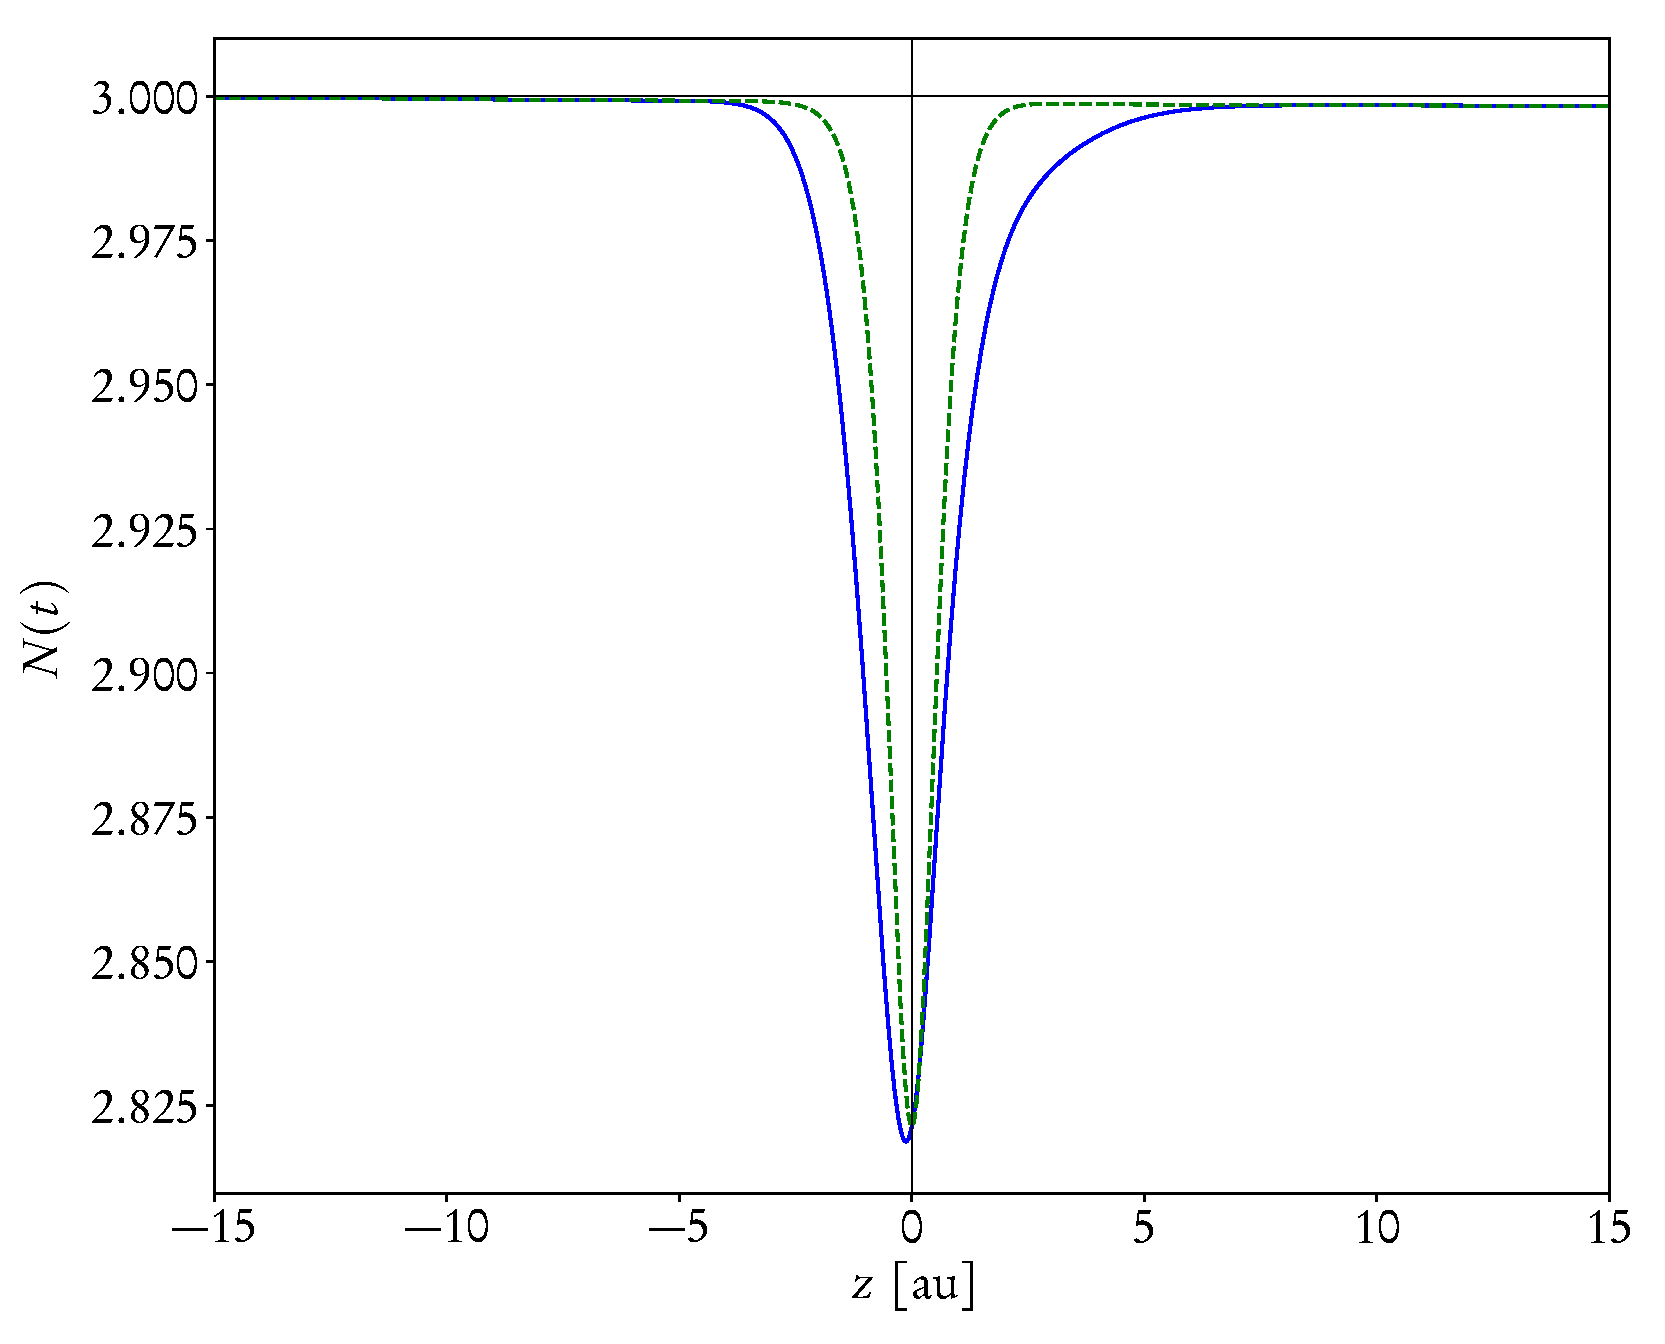
\includegraphics[width=\linewidth]{./images/toymodel/dNorm-1s-20.eps}
               \caption{$E_P = 20~\mathrm{keV}/\mathrm{amu}$. \label{fig:toy20}}
            \end{subfigure}%
            \begin{subfigure}{.5\textwidth}
               \centering
               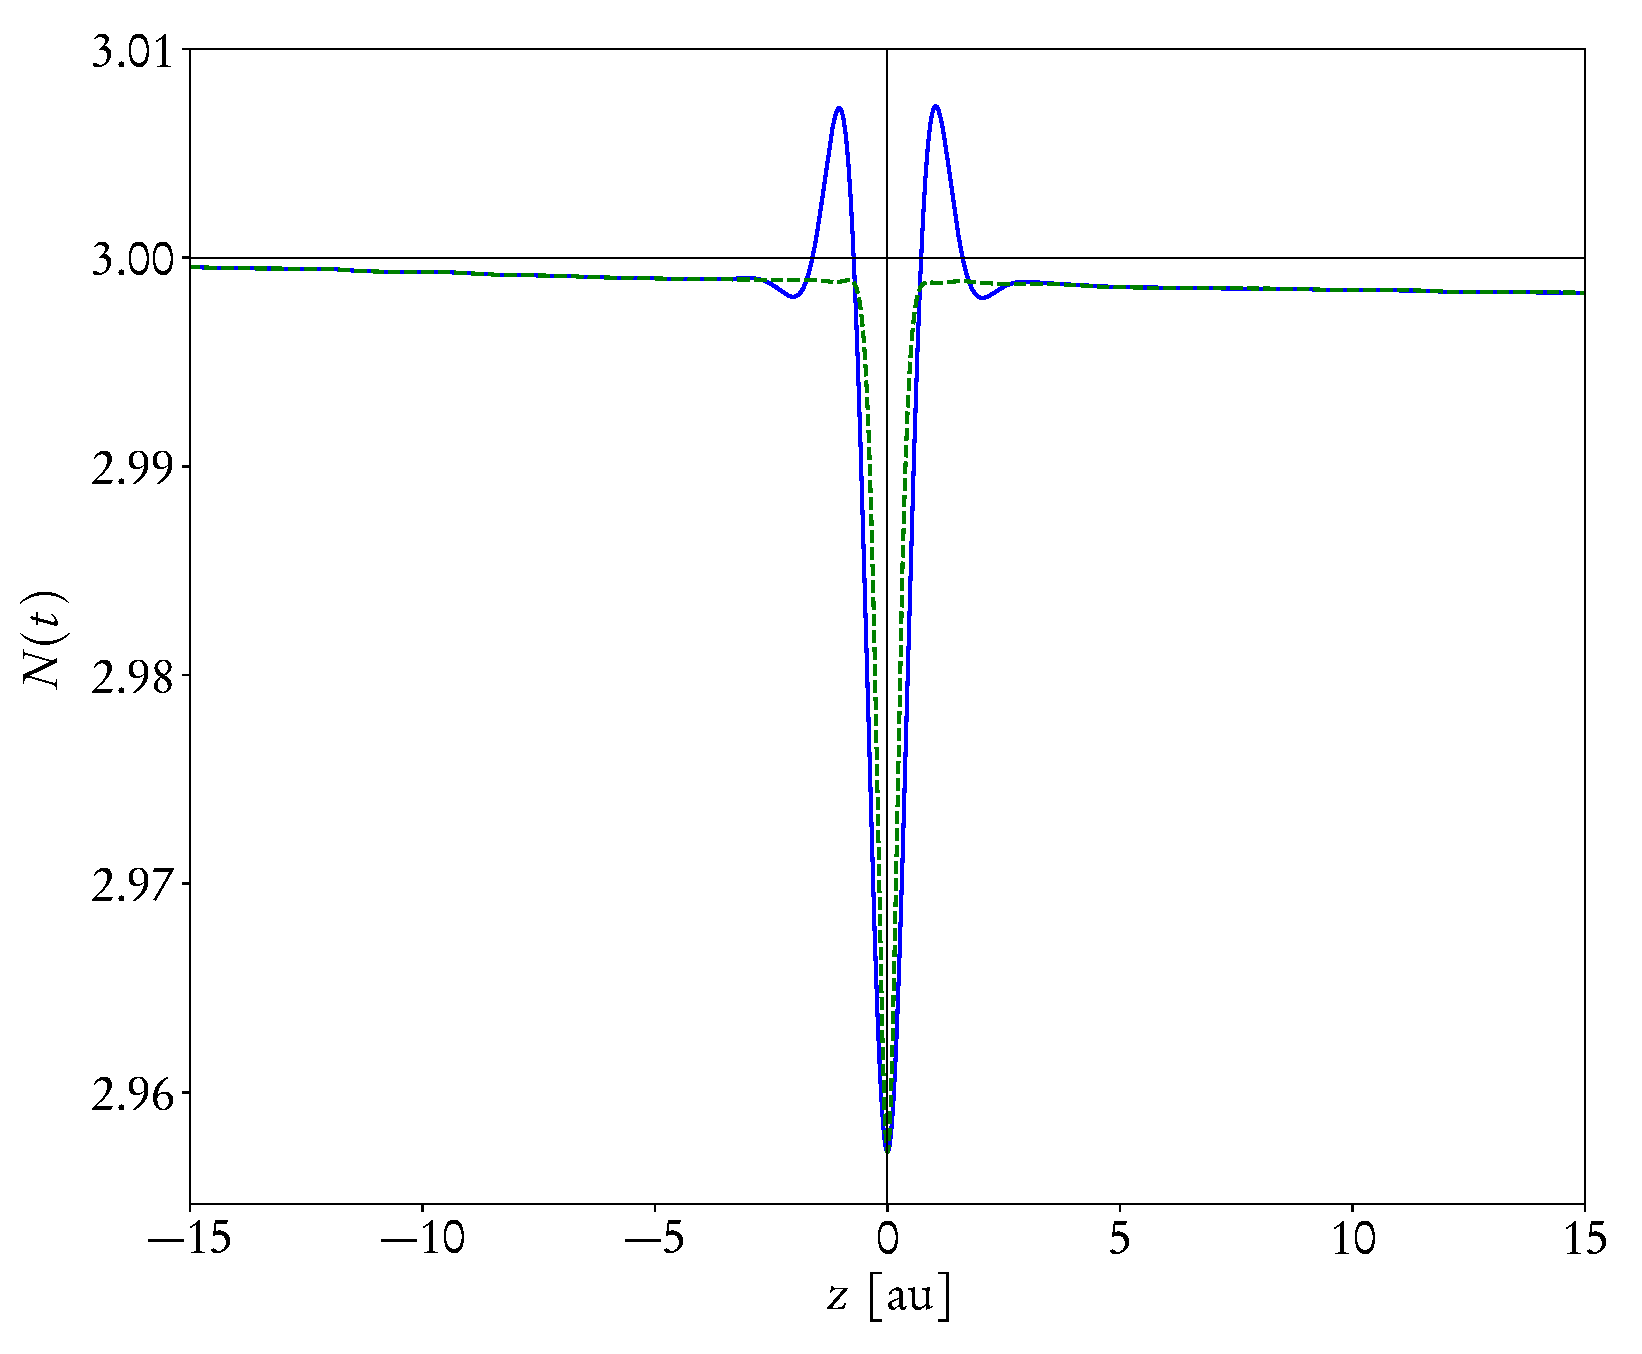
\includegraphics[width=\linewidth]{./images/toymodel/dNorm-1s-1000.eps}
               \caption{$E_P = 1000~\mathrm{keV}/\mathrm{amu}$. \label{fig:toy1000}}
            \end{subfigure}
            \caption[Number of particles as a function of \textit{z} in 1\textit{s}-only toy model]
                    {Number of particles as a function of $z$ in 1$s$-only toy model for $b = 1.0~
                    \mathrm{a.u}$. In both panels; solid line: \textsc{etf} off, dashed line:
                    partial \textsc{etf} on. \label{fig:toy}}
         \end{figure}

         Figures~\ref{fig:toy20} and \ref{fig:toy1000} display $N$ as a function of $z = Vt$ for
         collisions with impact energy of 20~keV/amu and 1000~keV/amu respectively. Both calculations
         including and excluding the partial \textsc{etf}s use an impact parameter of 1~a.u and include
         response. While both curves representing show sizable norm violations the inclusion of a
         partial \textsc{etf} offers clear benefits. The \textsc{etf}s reduce the overall size of the
         violations and reduce the range of time over which these violations occur. This can be seen
         most clearly in Fig.~\ref{fig:toy20} where the dashed curve detaches from the $N = 3$ line more
         slowly and reattaches more quickly. Additionally including \textsc{etf}s corrects the
         unexpected asymmetry about $z = 0$~a.u.

         The origins of the norm violations is easy to trace. According to Eq.~\eqref{eq:dendef2} the
         one-particle density may be written
         %
         \begin{equation} \label{eq:toyden}
            n(\mathbf{r},t) = \left| \varphi_{\uparrow 1}\right|^2
                            + \left| \varphi_{\uparrow 2}\right|^2
                            + \left| \varphi_{\downarrow 1}\right|^2.
         \end{equation}
         %
         Each orbital in the above expression is normalized to 1 and takes the form
         %
         \begin{equation}
            \varphi = a_T e^{i \mathbf{v}_T \cdot \mathbf{r}} \chi_T
                    + a_P e^{-i \mathbf{v}_T \cdot \mathbf{r}} \chi_P.
         \end{equation}
         %
         Every orbital then contributes
         %
         \begin{equation}
            \int \mathrm{d}^3 r \, \left| \varphi \right|^2 = \left| a_T \right|^2
                                                            + \left| a_P \right|^2
            + 2 \Re \left[ {a_T}^* a_P \tilde{S}_{TP} \right]
         \end{equation}
         %
         to $N$, where $\tilde{S}_{TP}$ are the matrix elements of the overlap matrix (including
         \textsc{etf}s). It can then be seen that norm violations are due to the fact that
         the \textsc{kli} cannot fully account for the overlaps of the \textsc{ks}-orbitals, a direct
         consequence of its inability to deal with non-cylindrically symmetric orbitals.

         The slight loss of norm noticeable in the tails of all four curves is on the order of $0.002$.
         One can consider the small violation as a limit on the accuracy of calculations. This error is
         on the order of $0.06 \%$.

      \end{subsection}

      \begin{subsection}{Impact Parameter Dependence}

         \begin{figure}[t]
            \centering
            \begin{subfigure}{.49\textwidth}
               \centering
               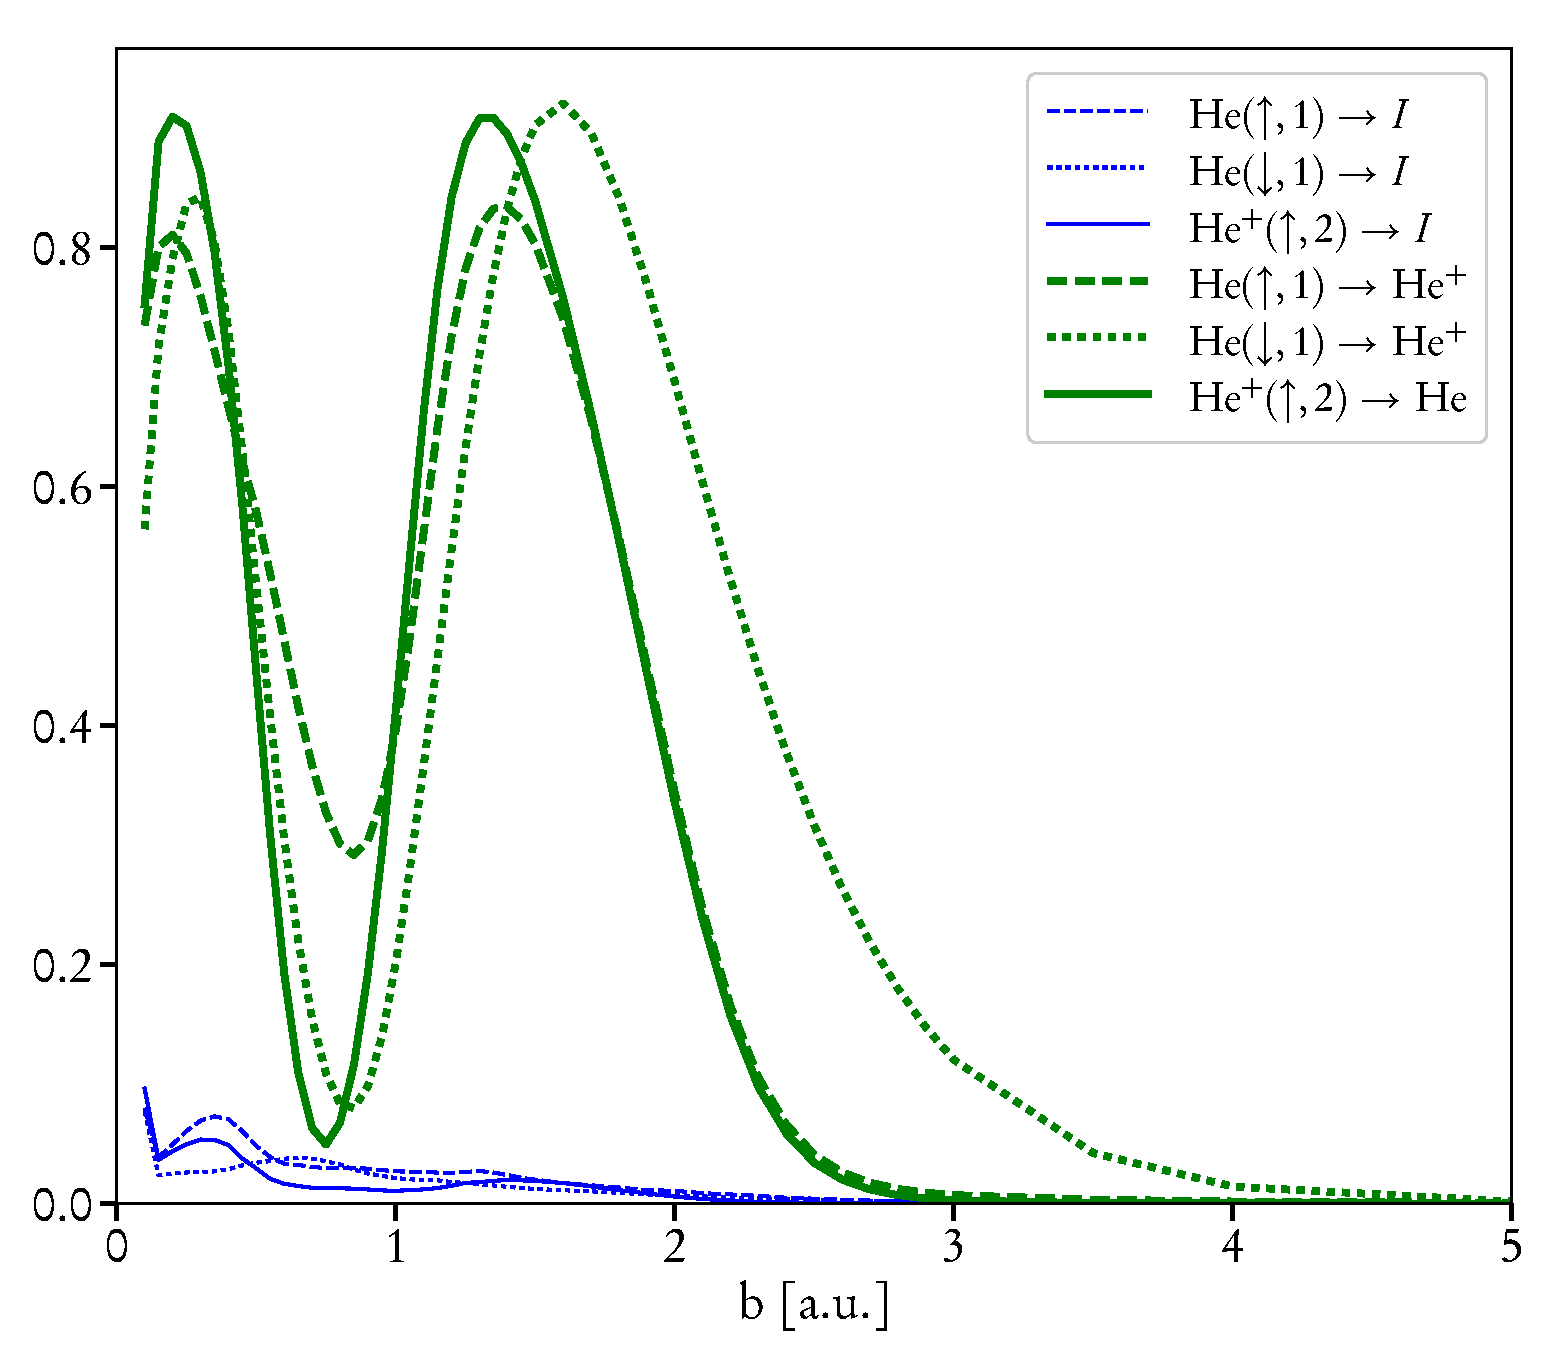
\includegraphics[width=\linewidth]{./images/hephe-bs/hepheTrans10.eps}
               \caption{$E_P = 10~\mathrm{keV}/\mathrm{amu}$. \label{fig:trans10}}
            \end{subfigure} \,
            \begin{subfigure}{.49\textwidth}
               \centering
               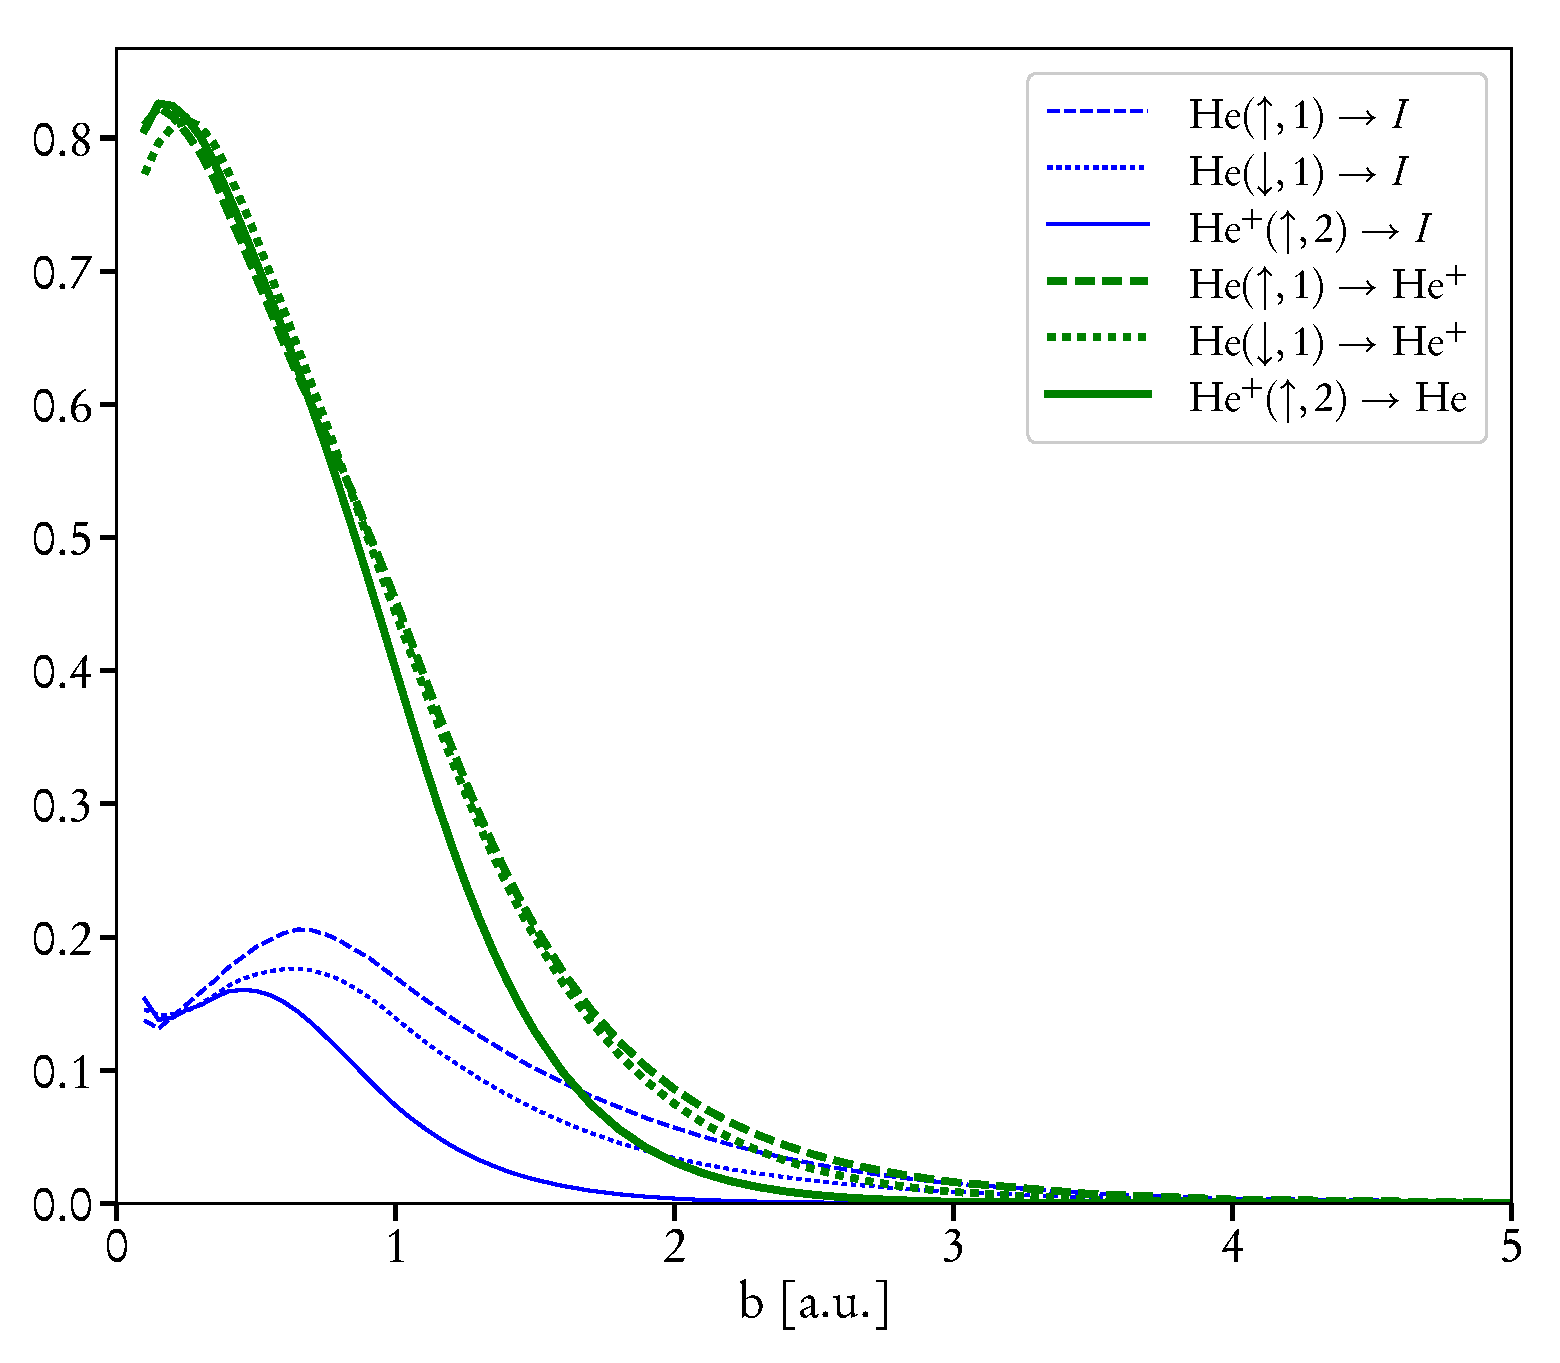
\includegraphics[width=\linewidth]{./images/hephe-bs/hepheTrans60.eps}
               \caption{$E_P = 60~\mathrm{keV}/\mathrm{amu}$. \label{fig:trans60}}
            \end{subfigure}

            \begin{subfigure}{.49\textwidth}
               \centering
               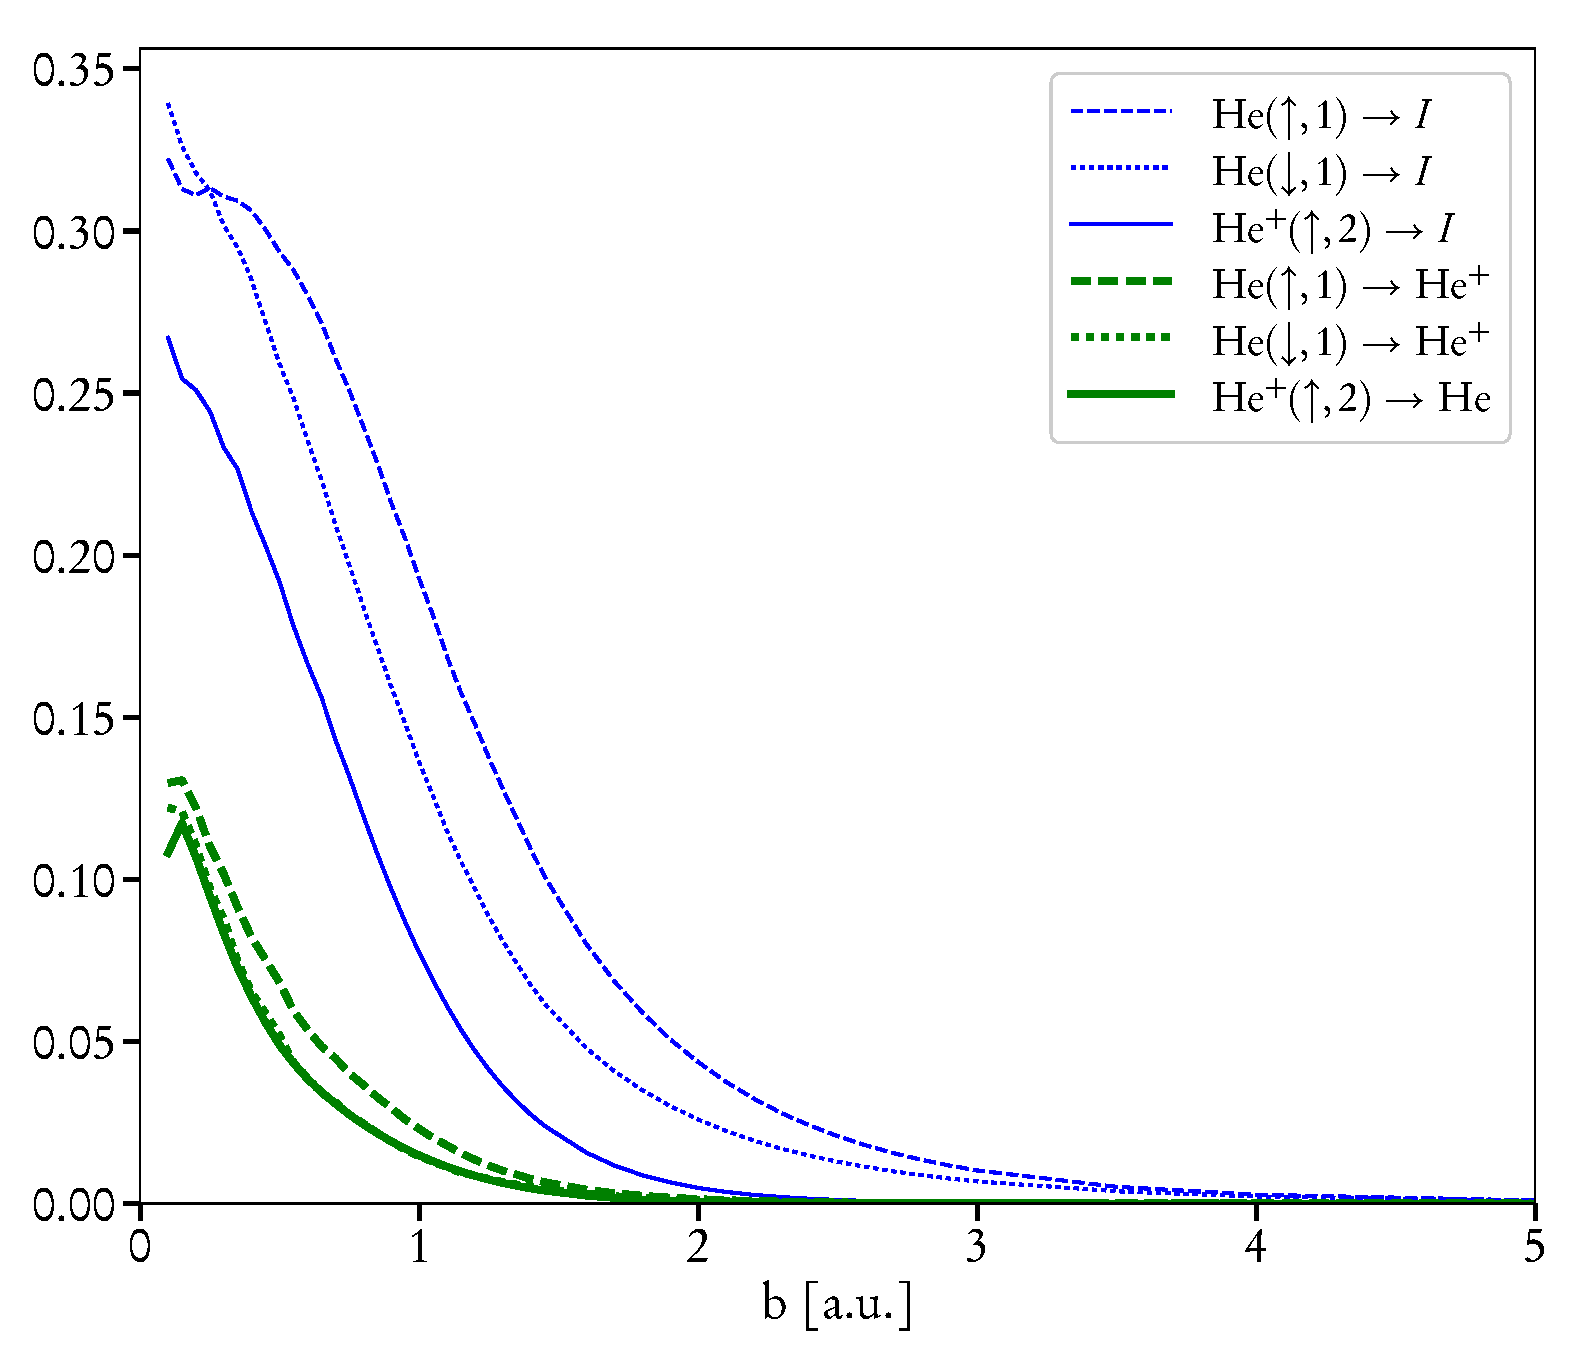
\includegraphics[width=\linewidth]{./images/hephe-bs/hepheTrans250.eps}
               \caption{$E_P = 250~\mathrm{keV}/\mathrm{amu}$. \label{fig:trans250}}
            \end{subfigure}
            \caption[Single-particle transfer and ionization and probabilities in
                     He\textsuperscript{+}-He collisions.]
                    {Single-particle transfer and ionization probabilities in
                     He\textsuperscript{+}-He collisions at various impact energies. \label{fig:trans}}
         \end{figure}

         Before discussing the total cross section results we will present some of the lower level
         features of the full calculations. We will consider the single-particle probabilities for each
         electron to ionize and to switch the nuclear centre to which it is bound. These probabilities
         can be calculated from the transition amplitudes. As an example, if $\varphi_{\uparrow 1}$
         begins initially on the target then the single-particle probability to ionize this electron can
         be written
         %
         \begin{equation} \label{eq:ionprob}
            p \left( \mathrm{He}(\uparrow_1) \rightarrow I \right) =
               \sum\limits_{c \in \{T,P\}} \sum\limits_{k=1}^K \sum\limits_{l = 1}^L
               \left| \braket{ \tilde{\chi}^{l0}_{c k} | \varphi_{\uparrow 1}(t_f)} \right|^2
         \end{equation}
         %
         and the single-particle probability to transfer to the projectile may be written
         %
         \begin{equation} \label{eq:transprob}
            p(\mathrm{He}(\uparrow_1) \rightarrow \mathrm{He}^+) =
               \sum\limits_{k=1}^K \left| \braket{ \tilde{\chi}^{00}_{P k} | \varphi_{\uparrow 1}(t_f)}
                          \right|^2,
         \end{equation}
         %
         where the probabilities are defined in terms of orthogonalized orbitals including full
         \textsc{etf}s. These probabilities are presented for the response model including partial
         \textsc{etf}s at the impact energies of 10, 60 and 250~keV/amu in Fig.~\ref{fig:trans}. When a
         distinction is made between response and no-response results the text refers to cross sections
         calculated using either set of fully time-dependent 1s-only orbitals and those using the model
         described in the text surrounding Eq.~\eqref{eq:noresp} respectively, when no distinction is
         made the text refers simply to the response versions.

         For low energy collisions capture processes can be seen to be dominant, this is clearly
         depicted in Fiq.~\ref{fig:trans10} where the single-particle ionization probabilities are
         negligible through the majority of impact parameters. In contrast, Fig.~\ref{fig:trans250}
         shows the diminishing importance of capture over ionization as impact energies increase.
         As one would expect the probability to ionize the more tightly bound He\textsuperscript{+}
         electron is consistently less than for either of the He electrons. Also of note is the obvious
         difference between the two He electrons, a clear reflection of the implementation of a
         spin-dependent potential.

         \begin{figure}[t]
            \centering
            \begin{subfigure}{.49\textwidth}
               \centering
               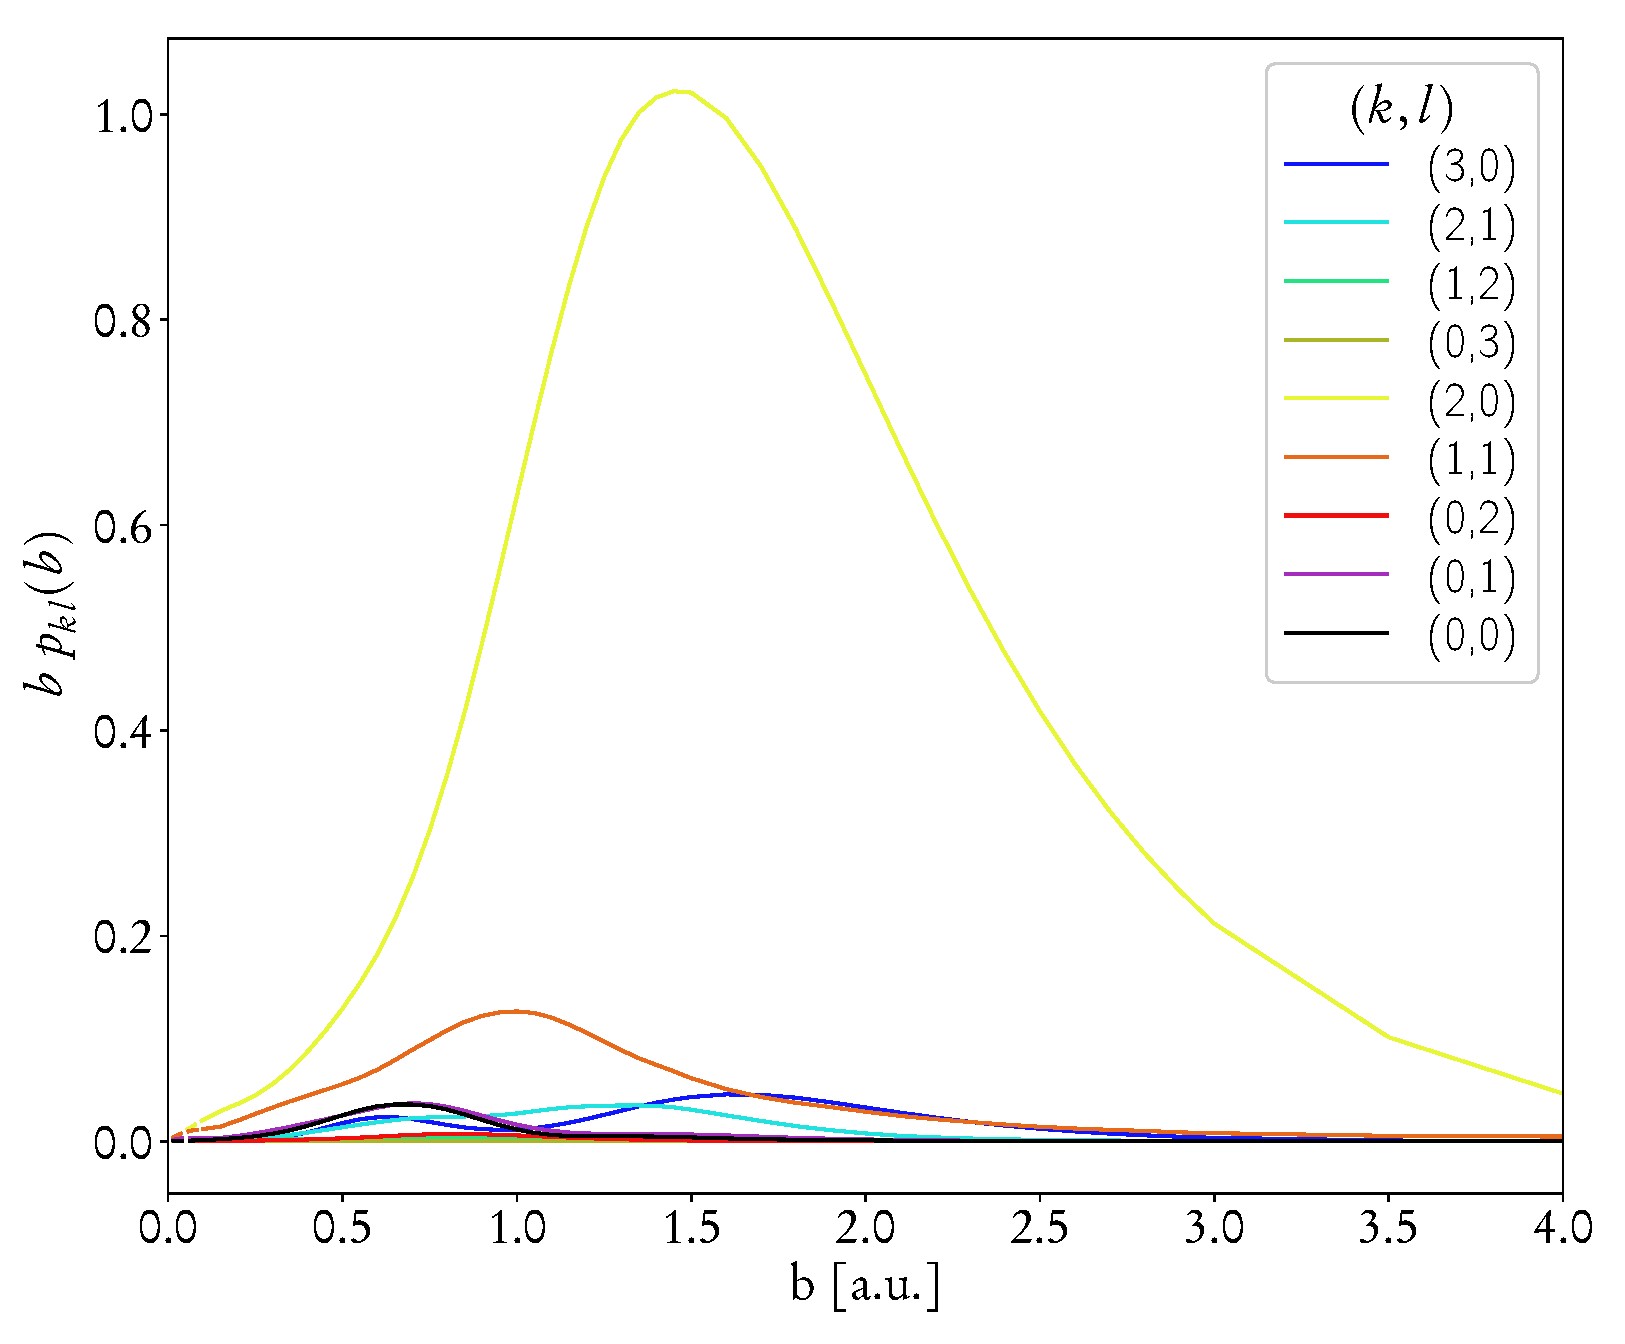
\includegraphics[width=\linewidth]{./images/hephe-bs/pkl-E20.eps}
               \caption{$E_P = 20~\mathrm{keV}/\mathrm{amu}$. \label{fig:pkl20}}
            \end{subfigure} \,
            \begin{subfigure}{.49\textwidth}
               \centering
               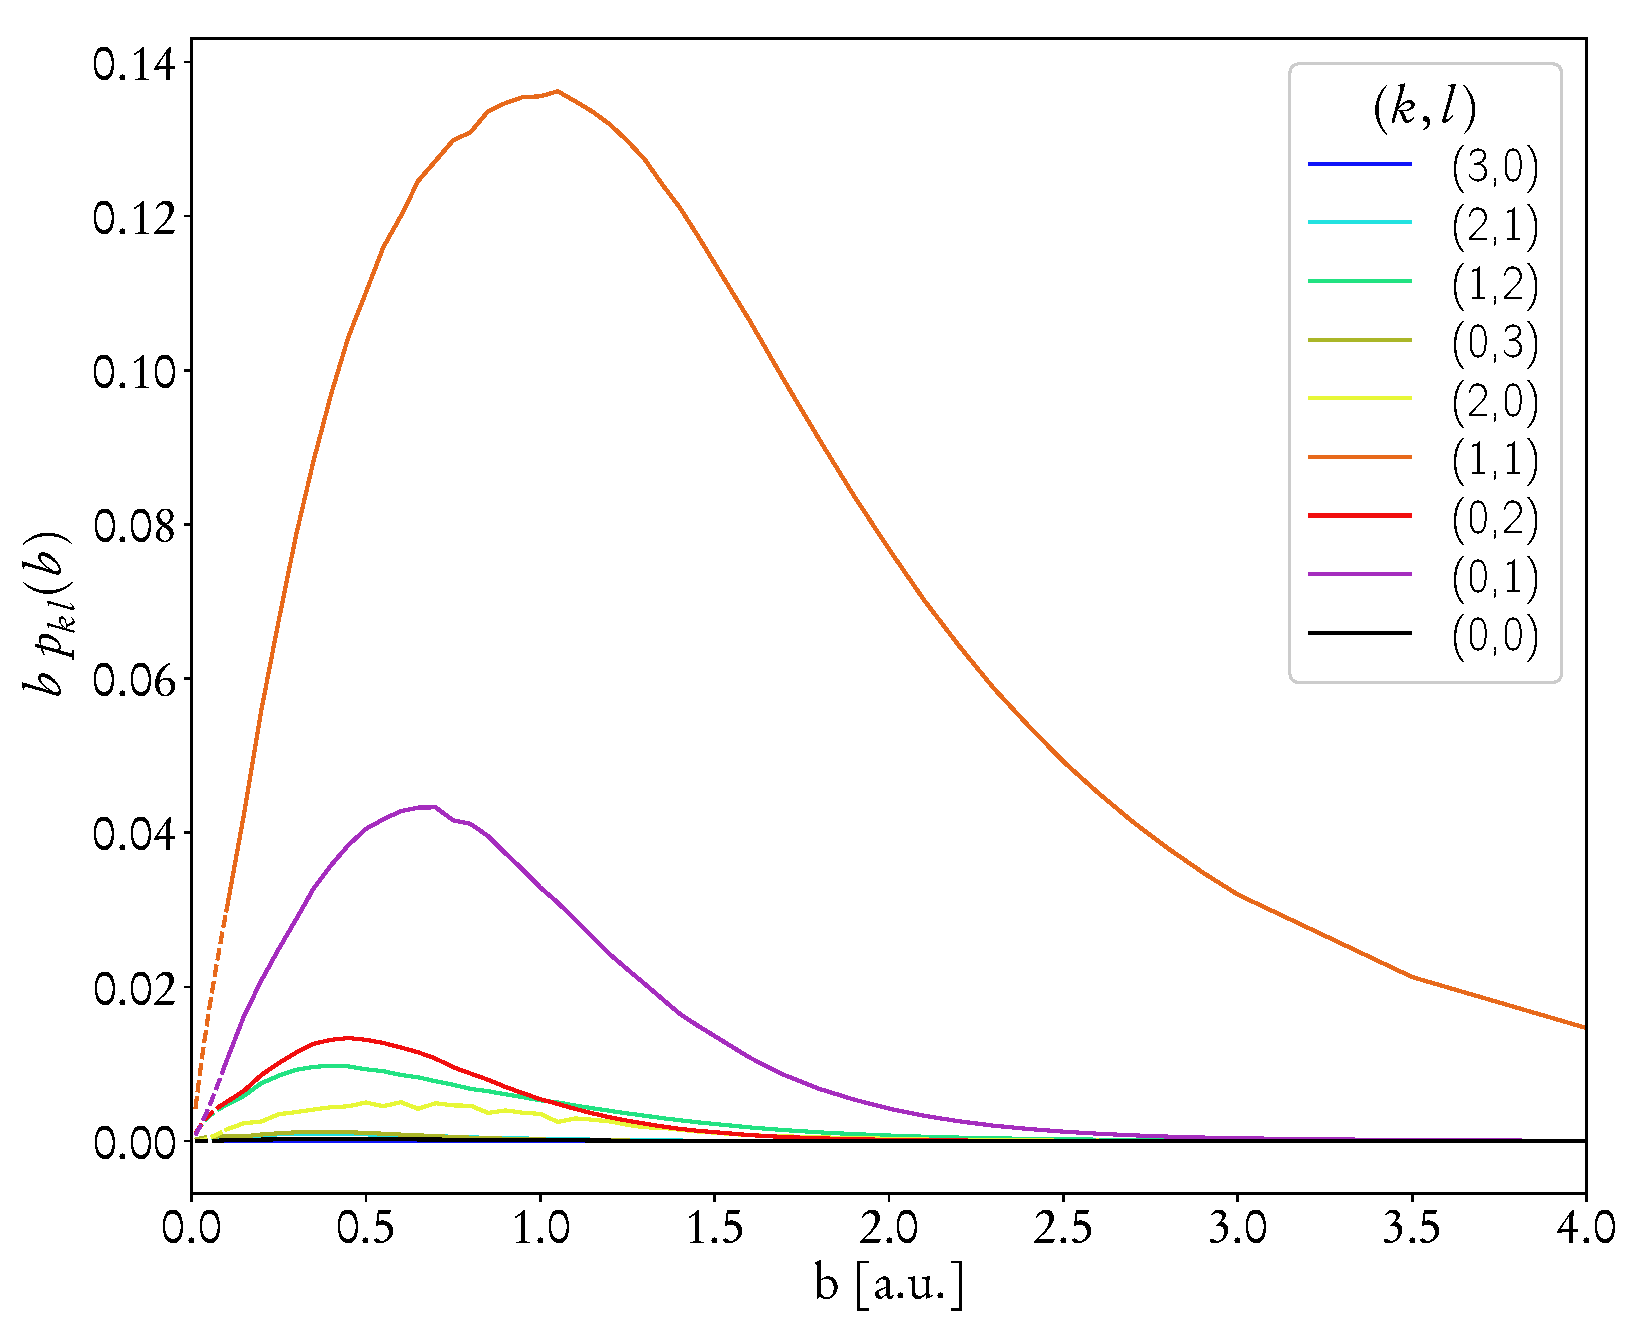
\includegraphics[width=\linewidth]{./images/hephe-bs/pkl-E500.eps}
               \caption{$E_P = 500~\mathrm{keV}/\mathrm{amu}$. \label{fig:pkl500}}
            \end{subfigure}

            \begin{subfigure}{.49\textwidth}
               \centering
               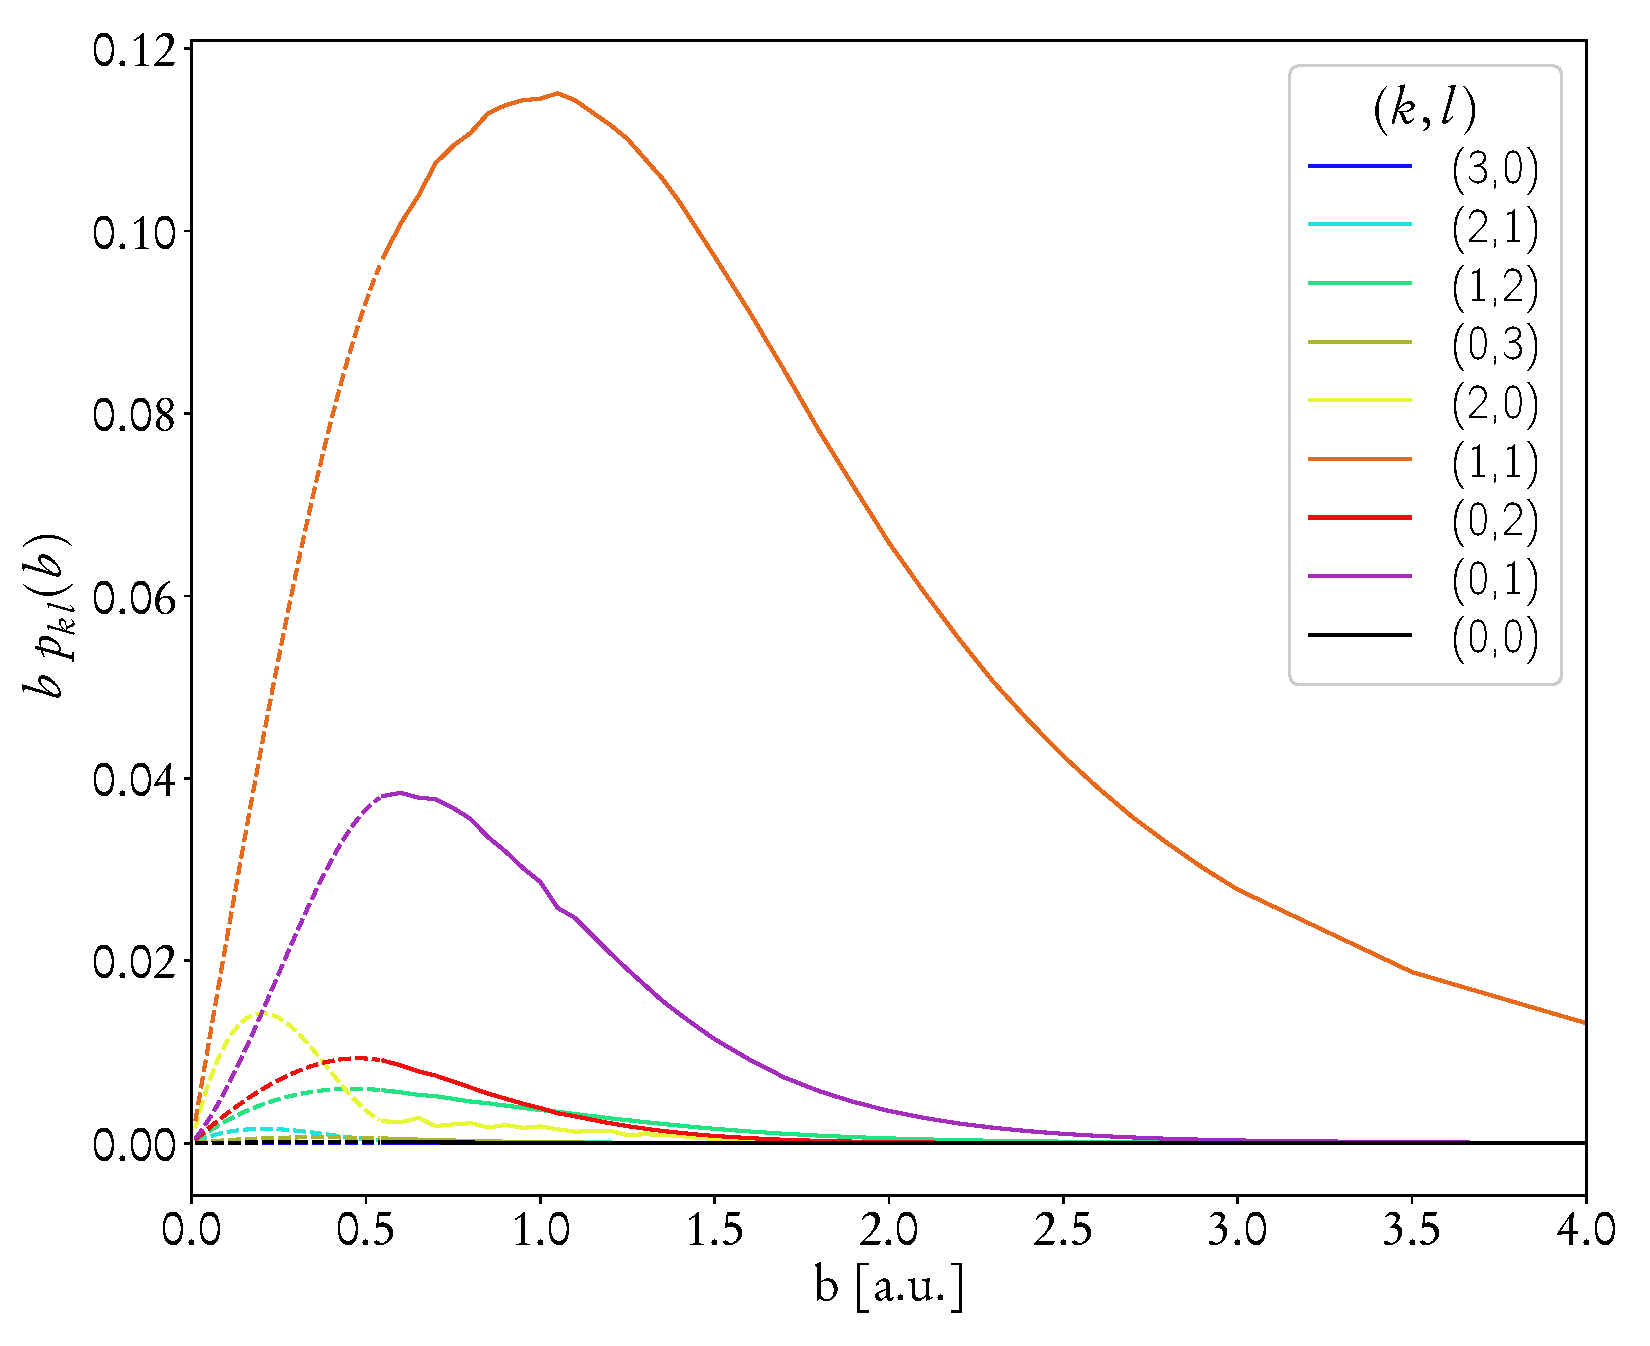
\includegraphics[width=\linewidth]{./images/hephe-bs/pkl-E600.eps}
               \caption{$E_P = 600~\mathrm{keV}/\mathrm{amu}$. \label{fig:pkl600}}
            \end{subfigure}
            \caption[Impact parameter dependent probabilities for all outcome channels in
                     He\textsuperscript{+}-He collisions]
                    {Impact parameter dependent probabilities for all outcome channels in
                     He\textsuperscript{+}-He collisions. Dashed portions of curves represent the region
                     where only the spline interpolant is available. \label{fig:pkl}}
         \end{figure}

         One last point must be mentioned before closing the discussion of impact parameter dependent
         probabilities. Presented in Fig.~\ref{fig:pkl} are integrands of Eq.~\eqref{eq:cross} for
         several impact energies, that is, impact parameter dependent probabilities for the outcome
         channels of Eqs.~\eqref{eq:tpi111}-\eqref{eq:tpi003} (with the addition of $p_{00}$ and
         $p_{30}$) times the impact parameter. For $E_p \leq$ 500~keV/amu the probabilities behave as
         one would expect. That is to say that the probabilities generally follow the relation $p(b)
         \sim b^n e^{-a b}$ for some integer $n$ and positive real number $a$. However, above this level
         unphysical structures begin to emerge. As an example the $p_{20}$ curve in
         Fig.~\ref{fig:pkl600} contains a large hump below 0.5~a.u.

         These are the result of numerical issues that limit the minimum possible impact parameter for
         which the calculations produce results from 0.1~a.u.\ below 500~keV/amu gradually to 0.8~a.u.\
         at 1000~keV/amu. In Eq.~\eqref{eq:cross} the integrand, $b \, p_{kl}(b)$, is approximated by a
         cubic spline which is, in turn, integrated to arrive at a cross section. The structure of the
         integrand means that so long as $p_{kl}(0)$ is finite its value is irrelevant and we always
         know the integrand at $b = 0$. In Fig.~\ref{fig:pkl} the solid portion of each curve represents
         the region where the probability may be determined at any point, the dashed sections represent
         the region where the spline interpolates between $b = 0$ and the next lowest available impact
         parameter. In the best possible scenario the lower bound on the error of a cubic spline will
         scale to the fourth power in the largest step between knots~\cite{spline-err}, for a spline
         $s_f$ interpolating a function $f$ one has
         %
         \begin{equation} \label{eq:splineErr}
            E(s_f) = \left| f - s_f \right|_\infty \leq \frac{5 \left| f^{(4)} \right|_\infty h^4}{384},
         \end{equation}
         %
         where $h$ is the largest separation between grid points used in determining the spline and
         %
         \begin{equation} \label{eq:supnorm}
            | g |_\infty = \sup\limits_{x \in [a,b]} \{ |g(x)| \}.
         \end{equation}
         %
         The step size factor in the error bound then increases from 0.0001 to 0.4096, an increase by an
         approximate factor of 4000. It is this decrease in the accuracy of the interpolation which
         results in the unphysical structures present in some outcome channels above 500~keV/amu. The
         presence of these structures are the reason for the lack of a data point at 800~keV/amu in
         Fig.~\ref{fig:cs201}, despite values having been calculated.

      \end{subsection}

      \begin{subsection}{Visualizing the Time-dependent Potential \label{sec:visual}}

         \begin{figure}[b]
            \centering
            \begin{subfigure}{.49\textwidth}
               \centering
               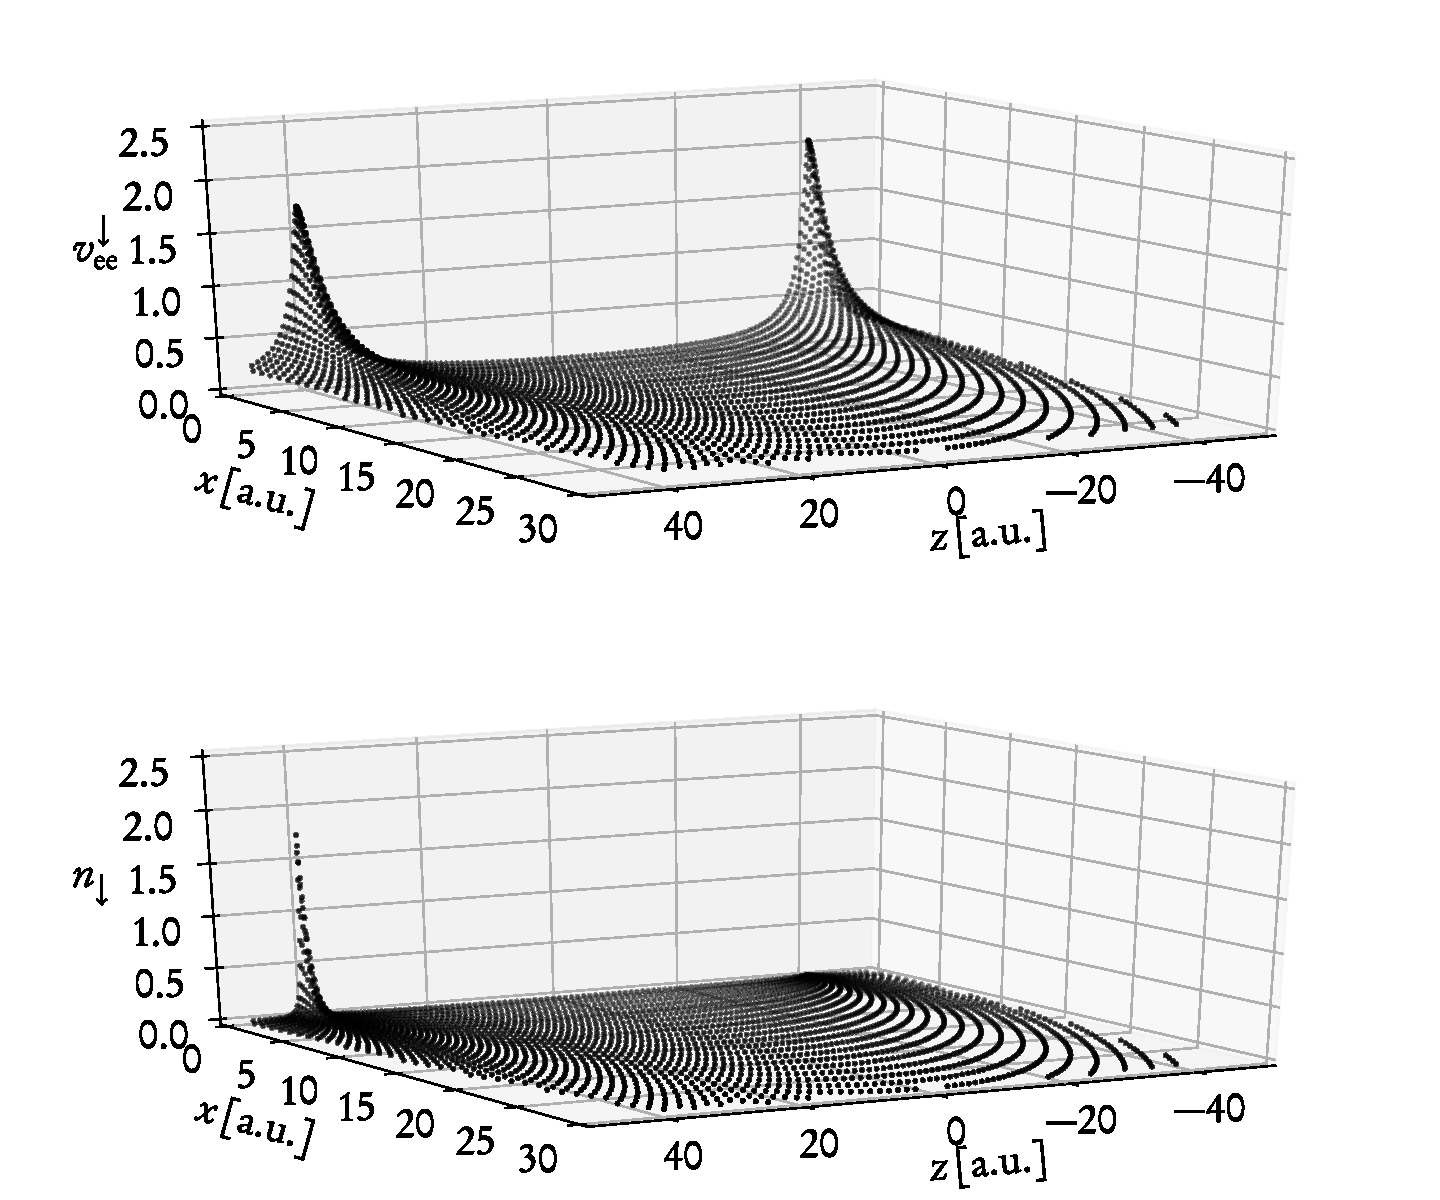
\includegraphics[width=\linewidth]{./images/frames/vee-dn-E50-b1-initial.pdf}
               \caption{$Z(t) = -40~\mathrm{a.u.}$. \label{fig:dnI}}
            \end{subfigure}
            \begin{subfigure}{.49\textwidth}
               \centering
               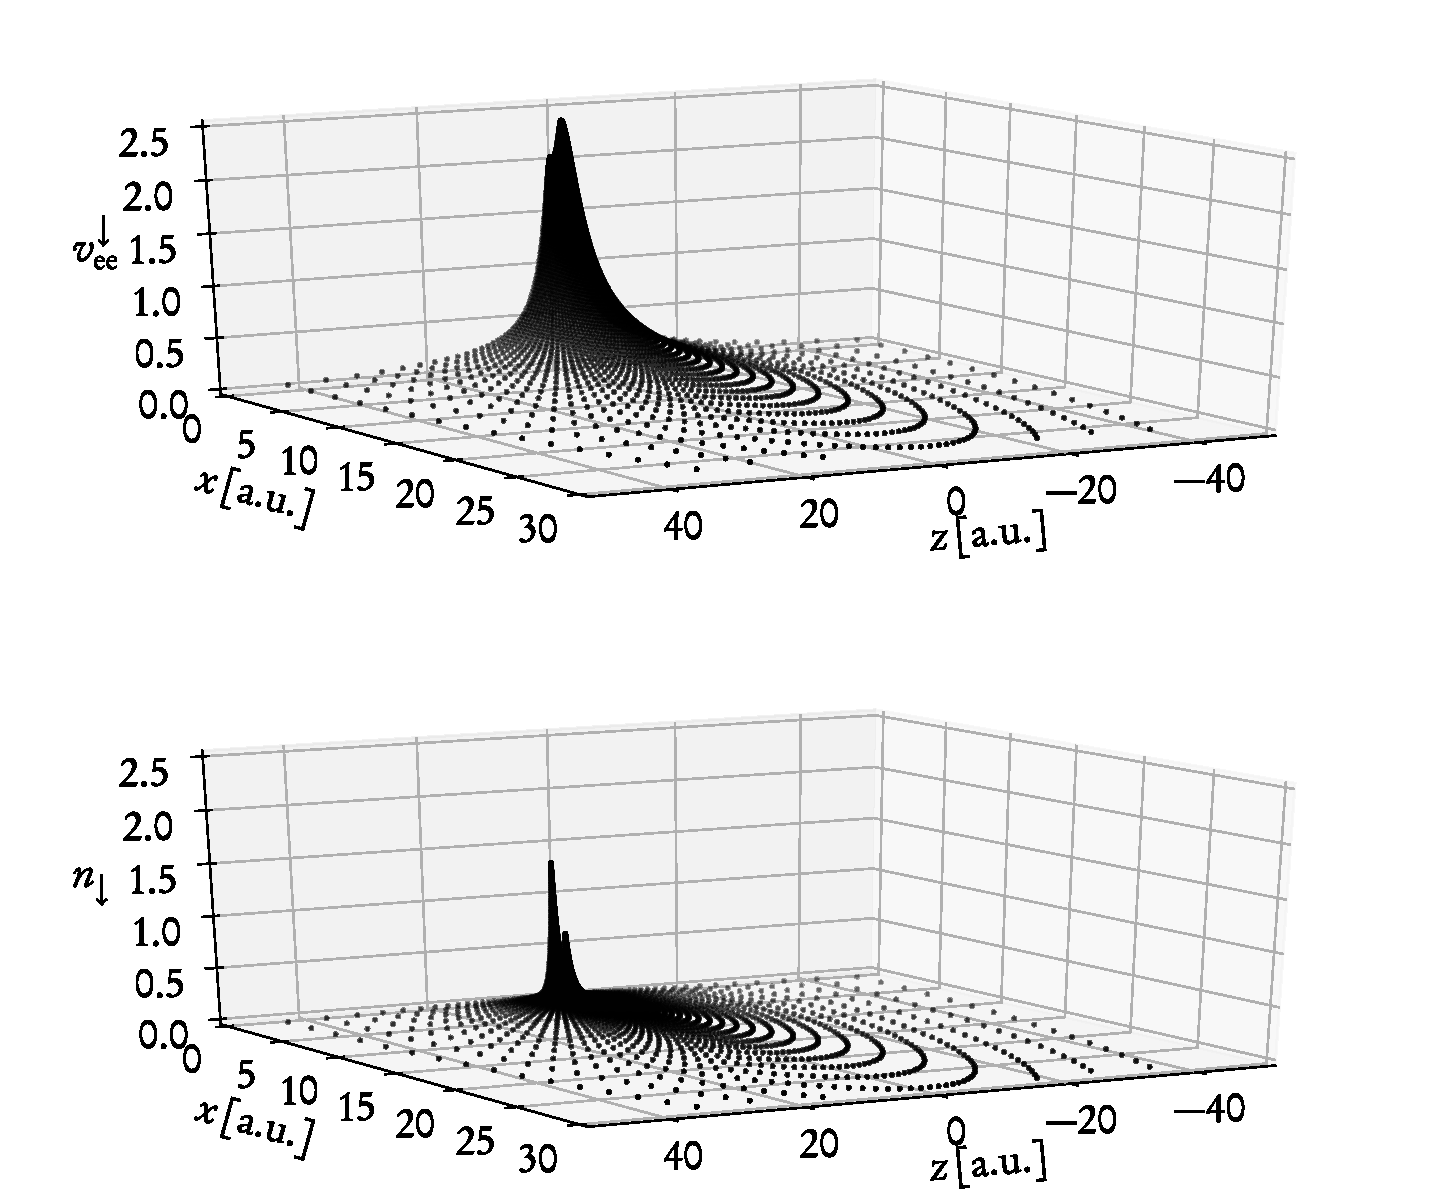
\includegraphics[width=\linewidth]{./images/frames/vee-dn-E50-b1-closest.pdf}
               \caption{$Z(t) = 0~\mathrm{a.u.}$. \label{fig:dnC}}
            \end{subfigure}
            \begin{subfigure}{.49\textwidth}
               \centering
               \includegraphics[width=\linewidth]{./images/frames/vee-dn-E50-b1-final.pdf}
               \caption{$Z(t) = 40~\mathrm{a.u.}$. \label{fig:dnF}}
            \end{subfigure}
            \caption[Spin-down electron-electron potential]
                    {Spin-down electron-electron potential compared with the spin-down component of the
                    one-particle density intially (a), at closest approach (b), and finally.
                    The parameters of the calculation are $E_P = 50~\mathrm{keV/amu}$ and
                    $b = 1.0~\mathrm{a.u.}$ \label{fig:dnPlots}}
         \end{figure}

         \begin{figure}[t]
            \centering
            \begin{subfigure}{.49\textwidth}
               \centering
               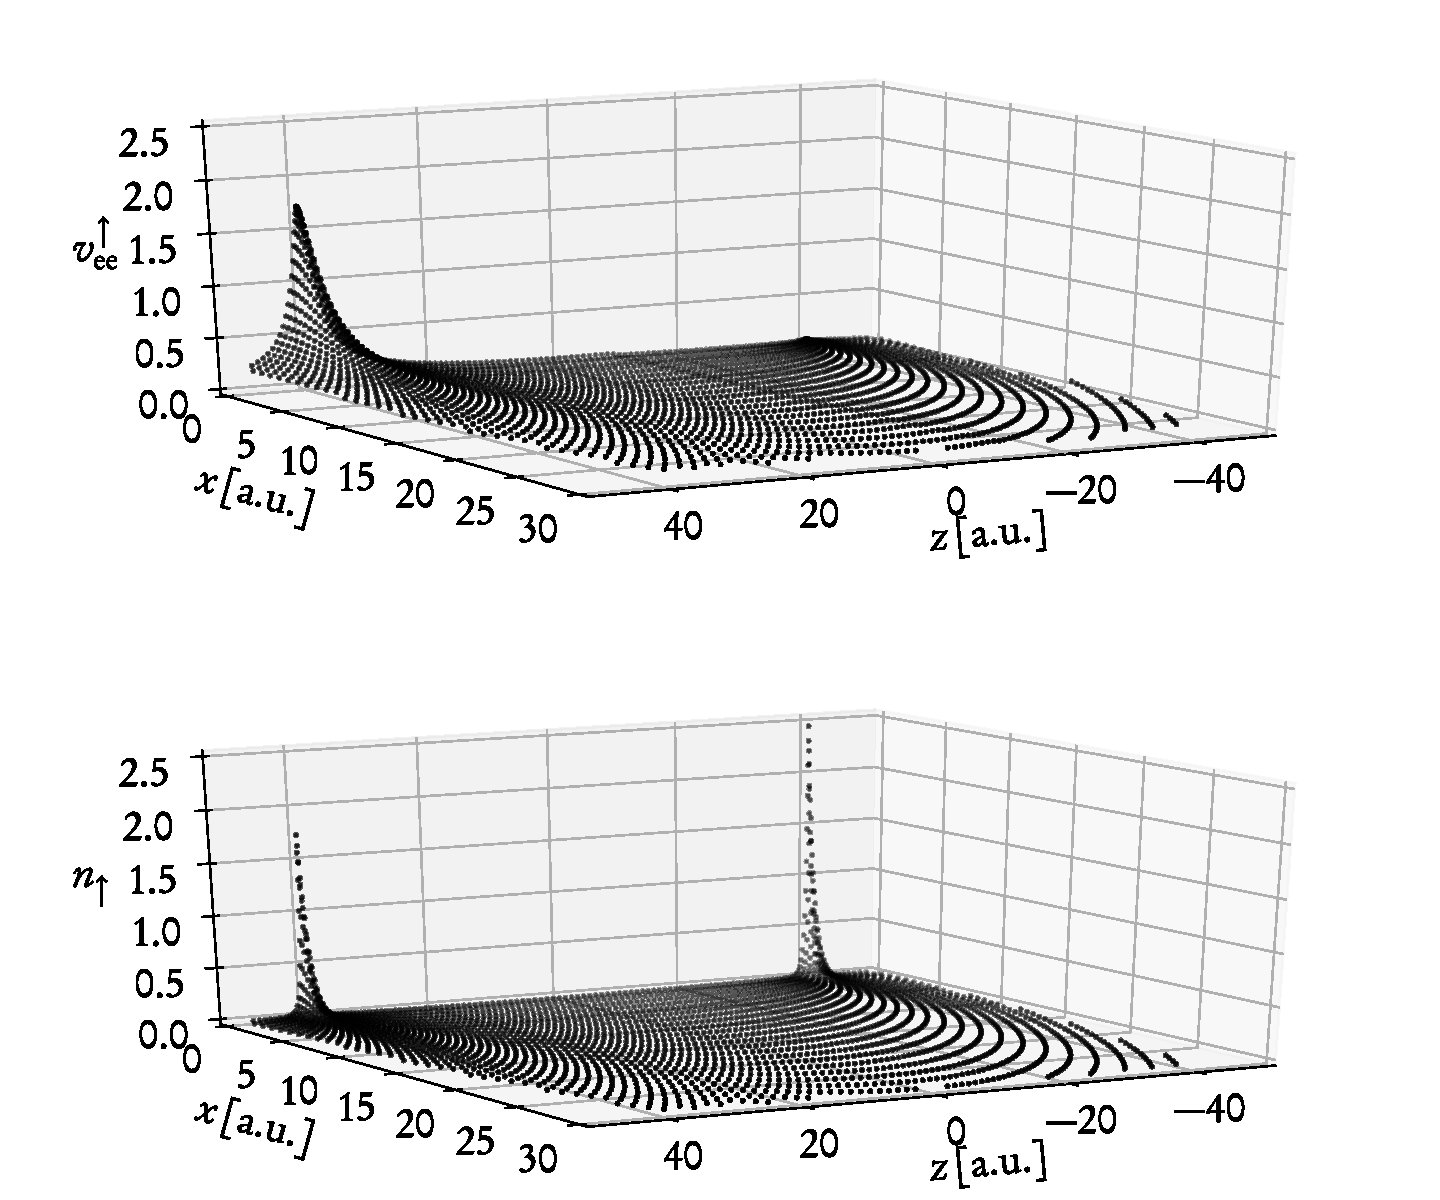
\includegraphics[width=\linewidth]{./images/frames/vee-up-E50-b1-initial.pdf}
               \caption{$Z(t) = -40~\mathrm{a.u.}$. \label{fig:upI}}
            \end{subfigure}
            \begin{subfigure}{.49\textwidth}
               \centering
               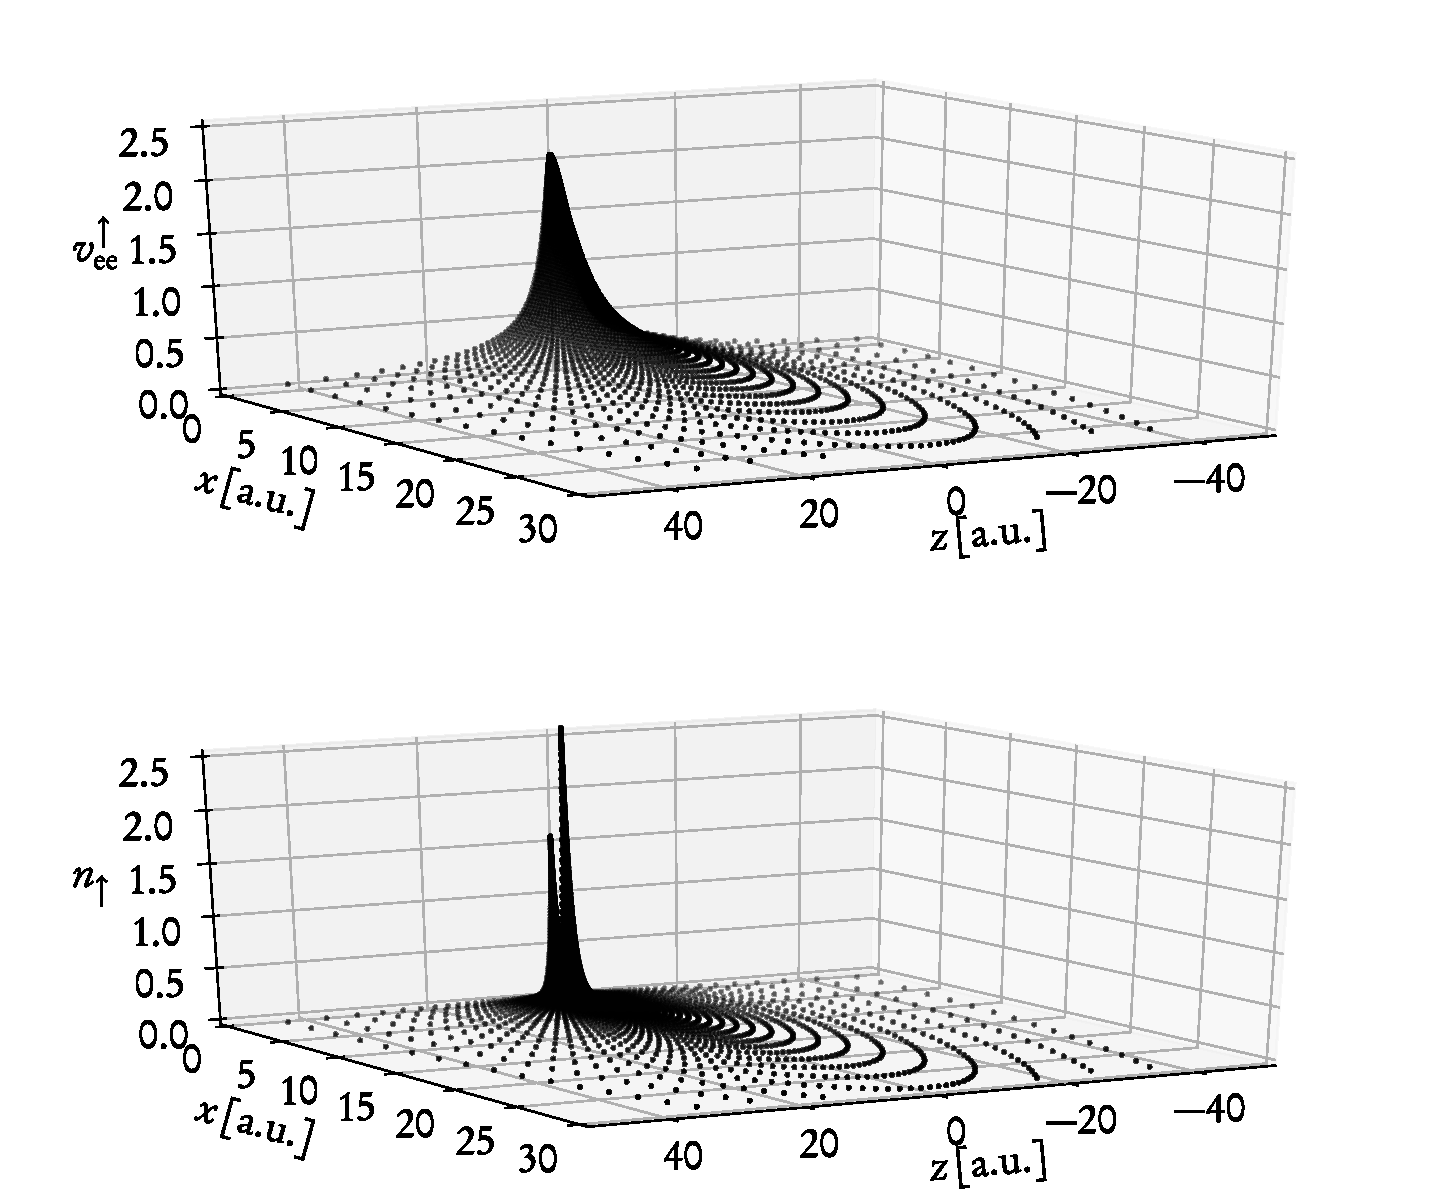
\includegraphics[width=\linewidth]{./images/frames/vee-up-E50-b1-closest.pdf}
               \caption{$Z(t) = 0~\mathrm{a.u.}$. \label{fig:upC}}
            \end{subfigure}
            \begin{subfigure}{.49\textwidth}
               \centering
               \includegraphics[width=\linewidth]{./images/frames/vee-up-E50-b1-final.pdf}
               \caption{$Z(t) = 40~\mathrm{a.u.}$. \label{fig:upF}}
            \end{subfigure}
            \caption[Spin-up electron-electron potential]
                    {Spin-up electron-electron potential compared with the spin-down component of the
                    one-particle density intially (a), at closest approach (b), and finally.
                    The parameters of the calculation are $E_P = 50~\mathrm{keV/amu}$ and
                    $b = 1.0~\mathrm{a.u.}$ \label{fig:upPlots}}
         \end{figure}

         If a picture is worth a thousand words then a thirty second long video at 24~fps is worth
         approximatetly 720 thousand words. To this end this appendix presents a collection of animations
         depicting the time evolution of the time-dependent \textsc{ks} potential. These videos may be
         found online\footnote{\url{https://tinyurl.com/ybo3yhqd}}.

         When visualizing the \textsc{ks} potential it is best to consider only the electron-electron
         contributions, that is to ignore the external potential. This is beneficial because from the
         perspective of the current work we are primarily interested in the performance of our
         approximation to these portions of the potential. As the behaviour of the internuclear potential
         is well established tracking it is of little value. Additionally, the poles of the Couloumb
         potential will drown out the electron electron effects. For these reasons we will concern
         ourselves with just the electron-electron contributions
         %
         \begin{equation}
            v_\mathrm{ee}^\sigma = v_\mathrm{x}^\sigma + v_\mathrm{H}.
         \end{equation}

         The the spin-dependent electron-electron potentials are best shown along with the associated
         spin-densities, $n_\sigma$ of Eq.~\eqref{eq:spinden} genereted from the $1s$-only orbitals in
         the p\textsc{etf} model. In this way one can more easily understand the appearance and time
         evolution of $v_\mathrm{ee}^\sigma$. For example, $v_\mathrm{ee}^\uparrow$ contain a single
         peak. This is due to the exact cancelation of self interaction that is present on the
         projectile centre where initially only one electron resides.

         Figures \ref{fig:dnPlots} and \ref{fig:upPlots} show a sample of several frames taken from the
         animation for an collision with an impact energy of 50~keV/amu and impact parameter of 1.0~a.u.
         These figures depict the collisions process at the initial separation (Figs.~\ref{fig:dnI} and
         \ref{fig:upI}), at closest approach (Figs.~\ref{fig:dnC} and \ref{fig:upC}), and at the final
         time step (Figs.~\ref{fig:dnF} and \ref{fig:upF}). The arrangement of the collision system is
         easily determine by combining the initial spin-up and spin-down frames. Both of the density
         plots have peaks on the left while only the spin-up density has a peak on the right clearly
         demonstrating that the target is on the left side of the figures (as these plots are presented
         in the rotating centre of mass frame the target and projectile remain on one side of the plane
         with the internuclear axis as normal).

         At closest approach in Fig.~\ref{fig:dnC} one may already see a
         second peak developing on the projectile as some of the norm is transfered between the collsion
         centres. This interpretation is cemented in Fig.~\ref{fig:dnF} where the one-particle density
         contains two distinct maxima.

         The spin-up channels appear less active. This can be through the fact that up to closest
         approach the size and shape of the two peaks appear unchanged, only their possistions are
         noticably different. In the final frame a decernable loss of norm from both centres is
         apparent. This may be seen as evidence that the Pauli exclusion promised by the x-potential is
         performing as advertised.

         \FloatBarrier

      \end{subsection}

      \begin{subsection}{Results \label{sec:hephe-res}}

         In what follows all results obtained by propagating the full \textsc{ks} orbitals in a
         potential generated from the 1s-only orbitals of Eq.~\eqref{eq:1sonly} that include no electron
         translation factors will be designated by n\textsc{etf}. Those obtained by an application of
         the same processes using the 1s-only orbitals, with partial \textsc{etf}s, of
         Eq.~\eqref{eq:1sonlyetf} will be referred to as p\textsc{etf}.

         Where available the results of the current work are compared with calculations of other groups.
         It should be noted that only those calculations that describe the system quantum mechanically
         were considered, that is to say works that employ approaches such as the classical trajectory
         Monte Carlo method~\cite{GMZ17}, the over the barrier model~\cite{CC-07}, or the Bohr–Lindhard
         model~\cite{DYC-08, DLZ-12} are not included.

         We will begin our discussion of the total cross section results with a broad overview comparing
         the response and no-response calculations. In general for the cross sections presented in
         Figs.~\ref{fig:cs111} through \ref{fig:cs030} the response calculations produce values that are
         noticeably lower with the exception of $\sigma_{01}$ and $\sigma_{00}$ (Figs.~\ref{fig:cs201}
         and \ref{fig:cs300} respectively). Where the $\sigma_{01}$ no-response curve drops below the
         response results would appear to coincide with a spike in the response $\sigma_{30}$ results
         (Fig.~\ref{fig:cs030}). The artificial nature of the $\sigma_{00}$ channel makes determining
         whether the lower result is desirable or not difficult. The only other channel, apart from
         $\sigma_{00}$, where the no-response calculations are in better agreement with experiment is
         $\sigma_{02}$, Fig.~\ref{fig:cs102}, where lowering the results moves the response curve below
         experiment. The addition of response effects causing a decrease in cross sections is a typical
         result, see for example Ref.~\cite{microresp}.

         As was mentioned above the primary purpose of the no-response model in the present context was
         as a test-bed for isolating the \textsc{etf}s from other phase factors. If we consider only the
         physical outcome channels, i.e.\ exclude $\sigma_{00}$ and $\sigma_{03}$, a clear pattern
         emerges. For low impact energies the n\textsc{etf} and p\textsc{etf} curves coincide, what one
         would expect as $V$ approaches zero. As the impact energy increases a gap begins to open
         between the two sets of results. The only exceptions to this trend are $\sigma_{20}$
         (Fig.~\ref{fig:cs120}), where the cross sections are likely too large for small distinctions to
         be apparent, and $\sigma_{01}$ (Fig.~\ref{fig:cs201}) where the n\textsc{etf} and p\textsc{etf}
         response curves are slightly erratic. Leaving aside this channel the tendencies of the response
         and no-response models in the presence, or absence, of the partial \textsc{etf}s are
         essentially identical. From the discussion in Sec.~\ref{sec:toy} it is clear that the
         \textsc{etf}s have no effect on $v_\mathrm{H}$ in the no-response model. One can interpret this
         to mean that the differences between the n\textsc{etf} and p\textsc{etf} results are primarily
         attributable to the \textsc{etf}s and not the result of some unforeseen additional processes.

         \begin{figure}[t]
            \centering
            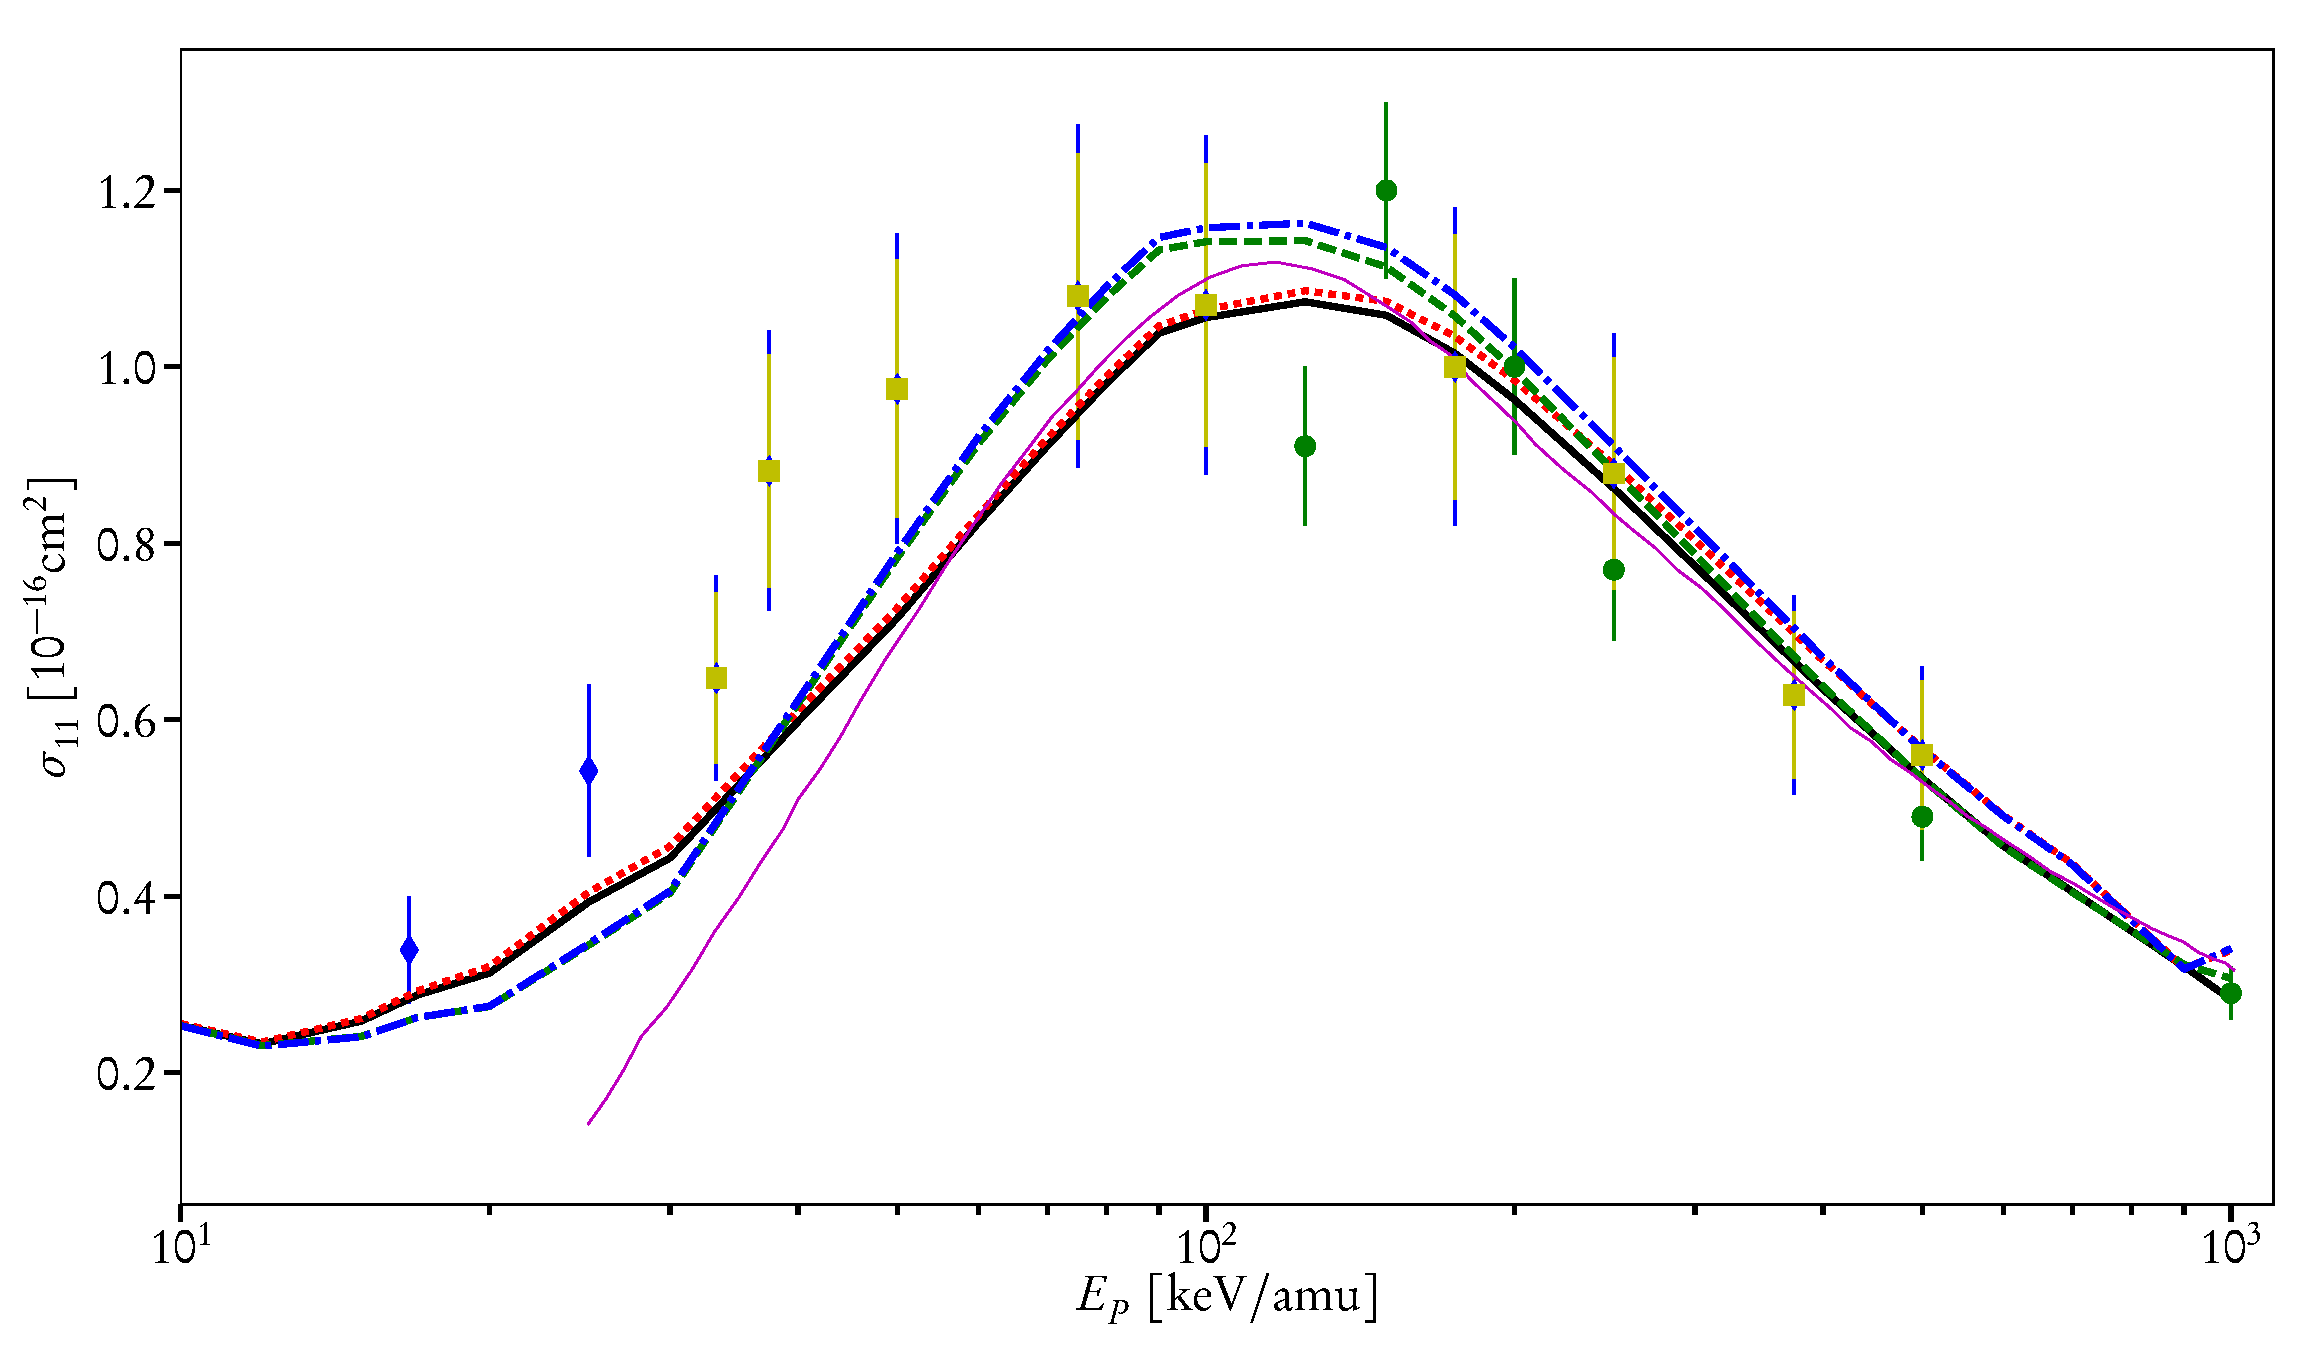
\includegraphics[width = \linewidth]{./images/hephe-cross/HepHe-111.eps}
            \caption[Total cross section for single ionization of the target in He\textsuperscript{+}-He
                     collisions.]
                    {Total cross section for single ionization of the target.
                     Theoretical results: p\textsc{etf} response (solid line), n\textsc{etf} response
                                          (dotted line), p\textsc{etf} no-response (dashed line),
                                          n\textsc{etf} no-response (dash-dotted line), and
                                          \textsc{cdw-eis} of Miraglia and Gravielle~\cite{MG-10}
                                          (thin solid line).
                     Experimental data: diamonds~\cite{Dub-89}, circles~\cite{FTFHLP-95}, and
                                        squares~\cite{DT-88}.
                     \label{fig:cs111}}
         \end{figure}

         \begin{figure}[t]
            \centering
            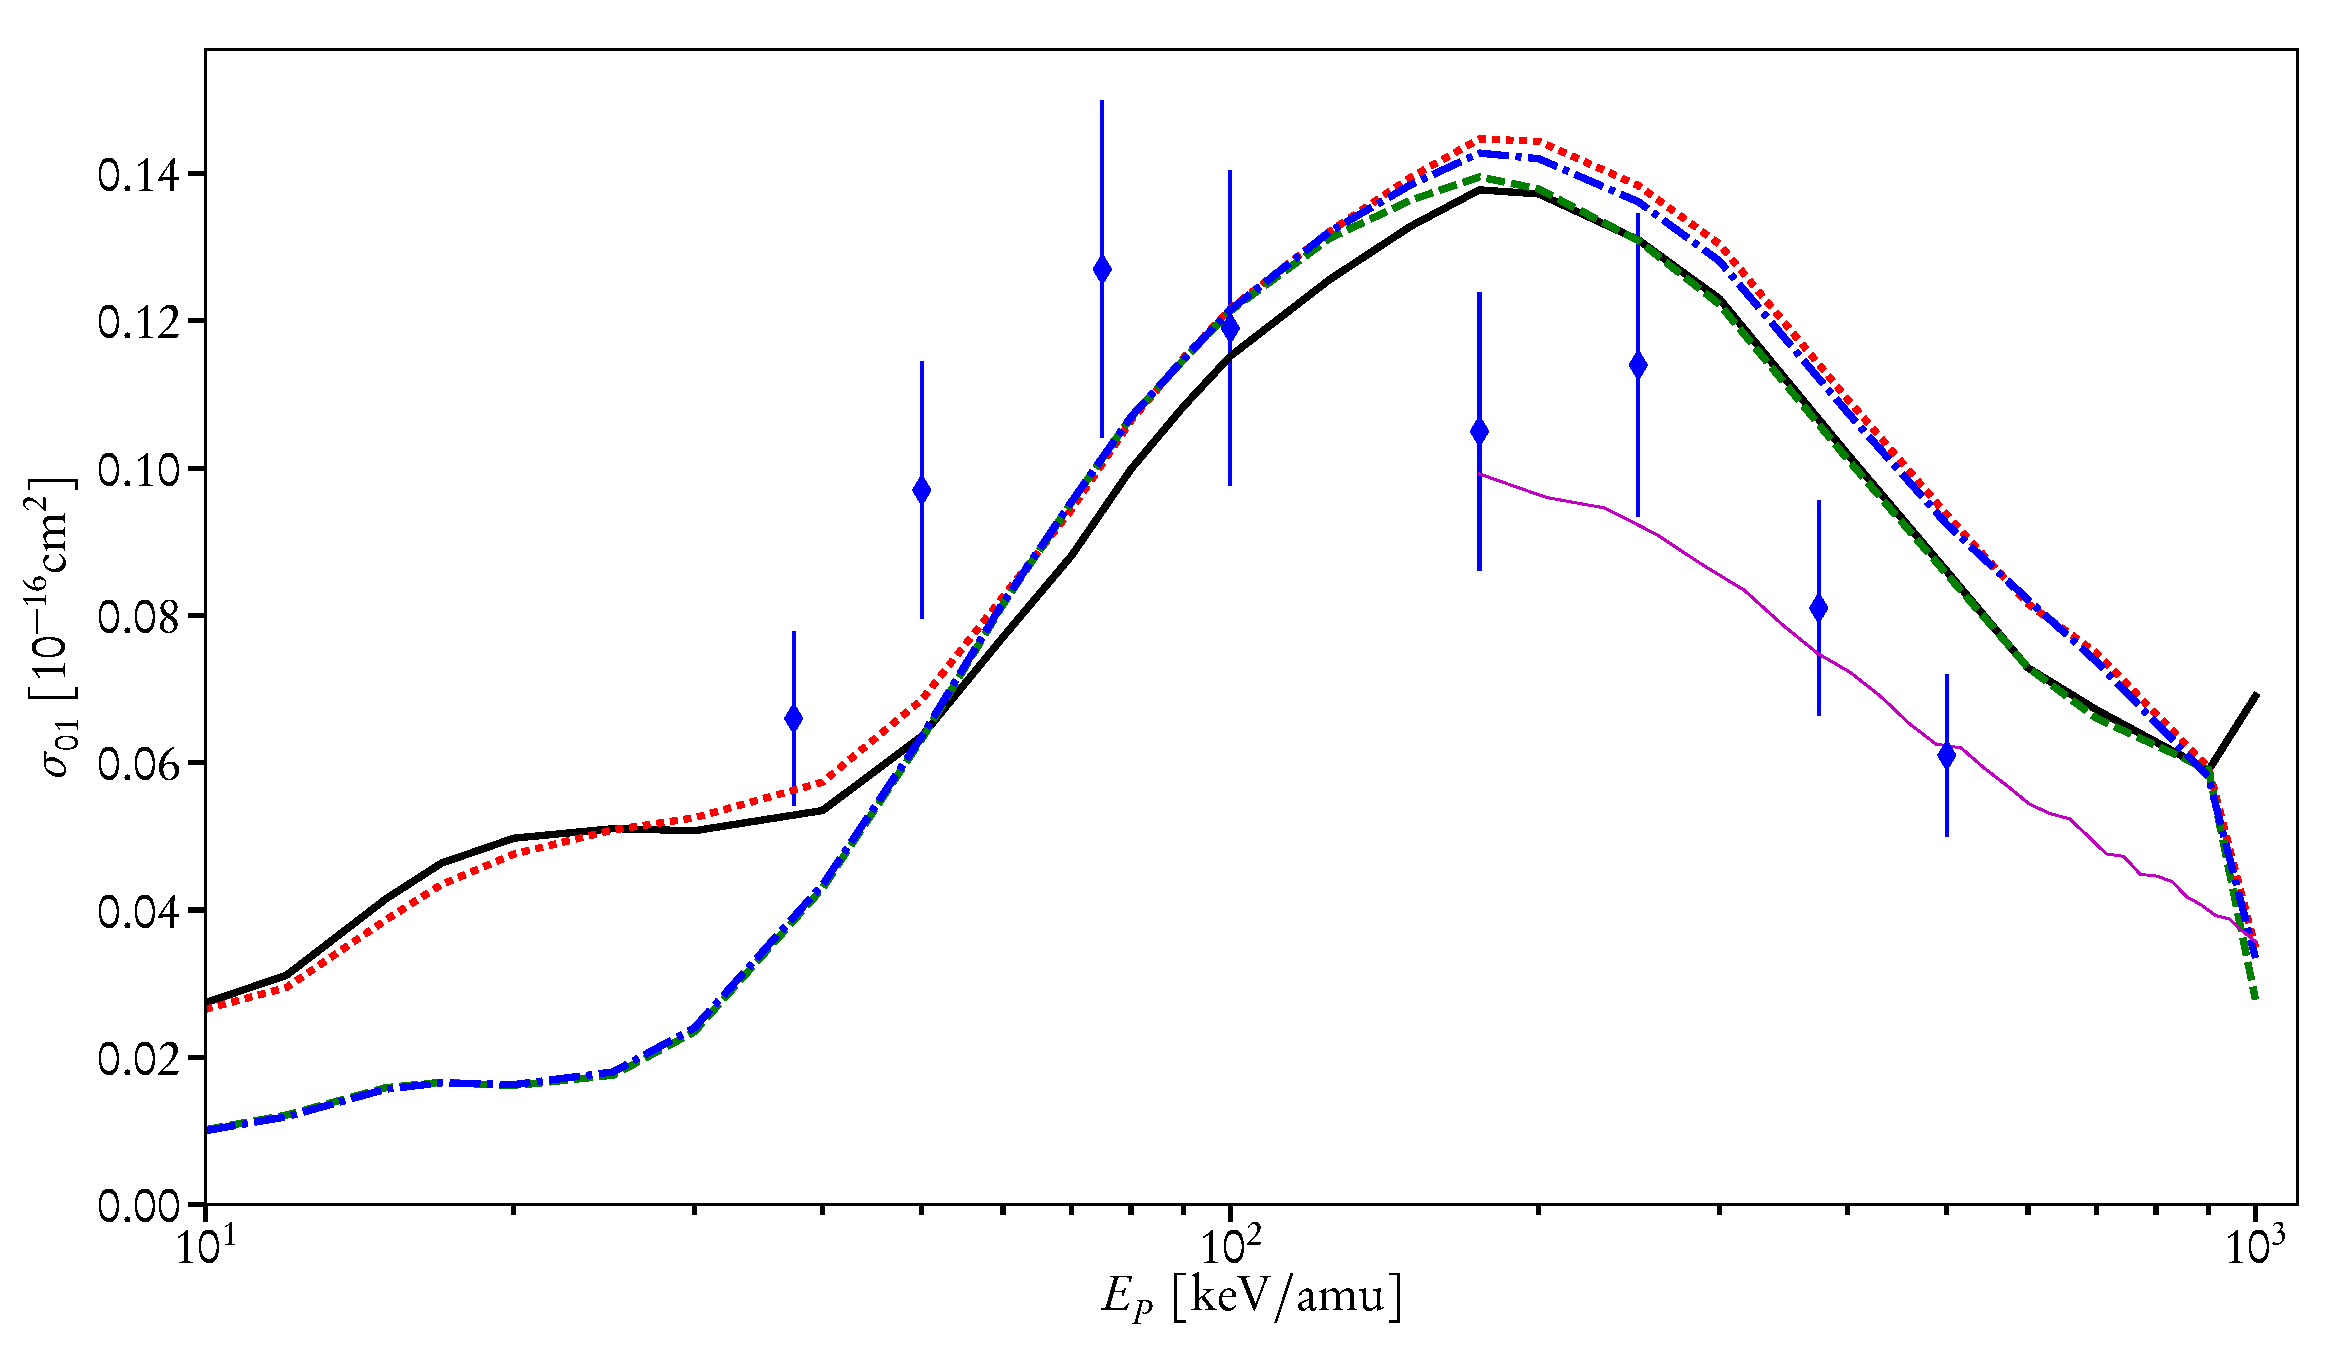
\includegraphics[width = \linewidth]{./images/hephe-cross/HepHe-201.eps}
            \caption[Total cross section for single ionization of the projectile in
                     He\textsuperscript{+}-He collisions.]
                    {Total cross section for single ionization of the projectile.
                     Theoretical results: p\textsc{etf} response (solid line), n\textsc{etf} response
                                          (dotted line), p\textsc{etf} no-response (dashed line),
                                          n\textsc{etf} no-response (dash-dotted line), and
                                          \textsc{ievm} of Sigaud and Montenegro~\cite{SM-03}
                                          (dash-dotted line).
                     Experimental data: diamonds~\cite{Dub-89}. \label{fig:cs201}}
         \end{figure}

         \begin{figure}[t]
            \centering
            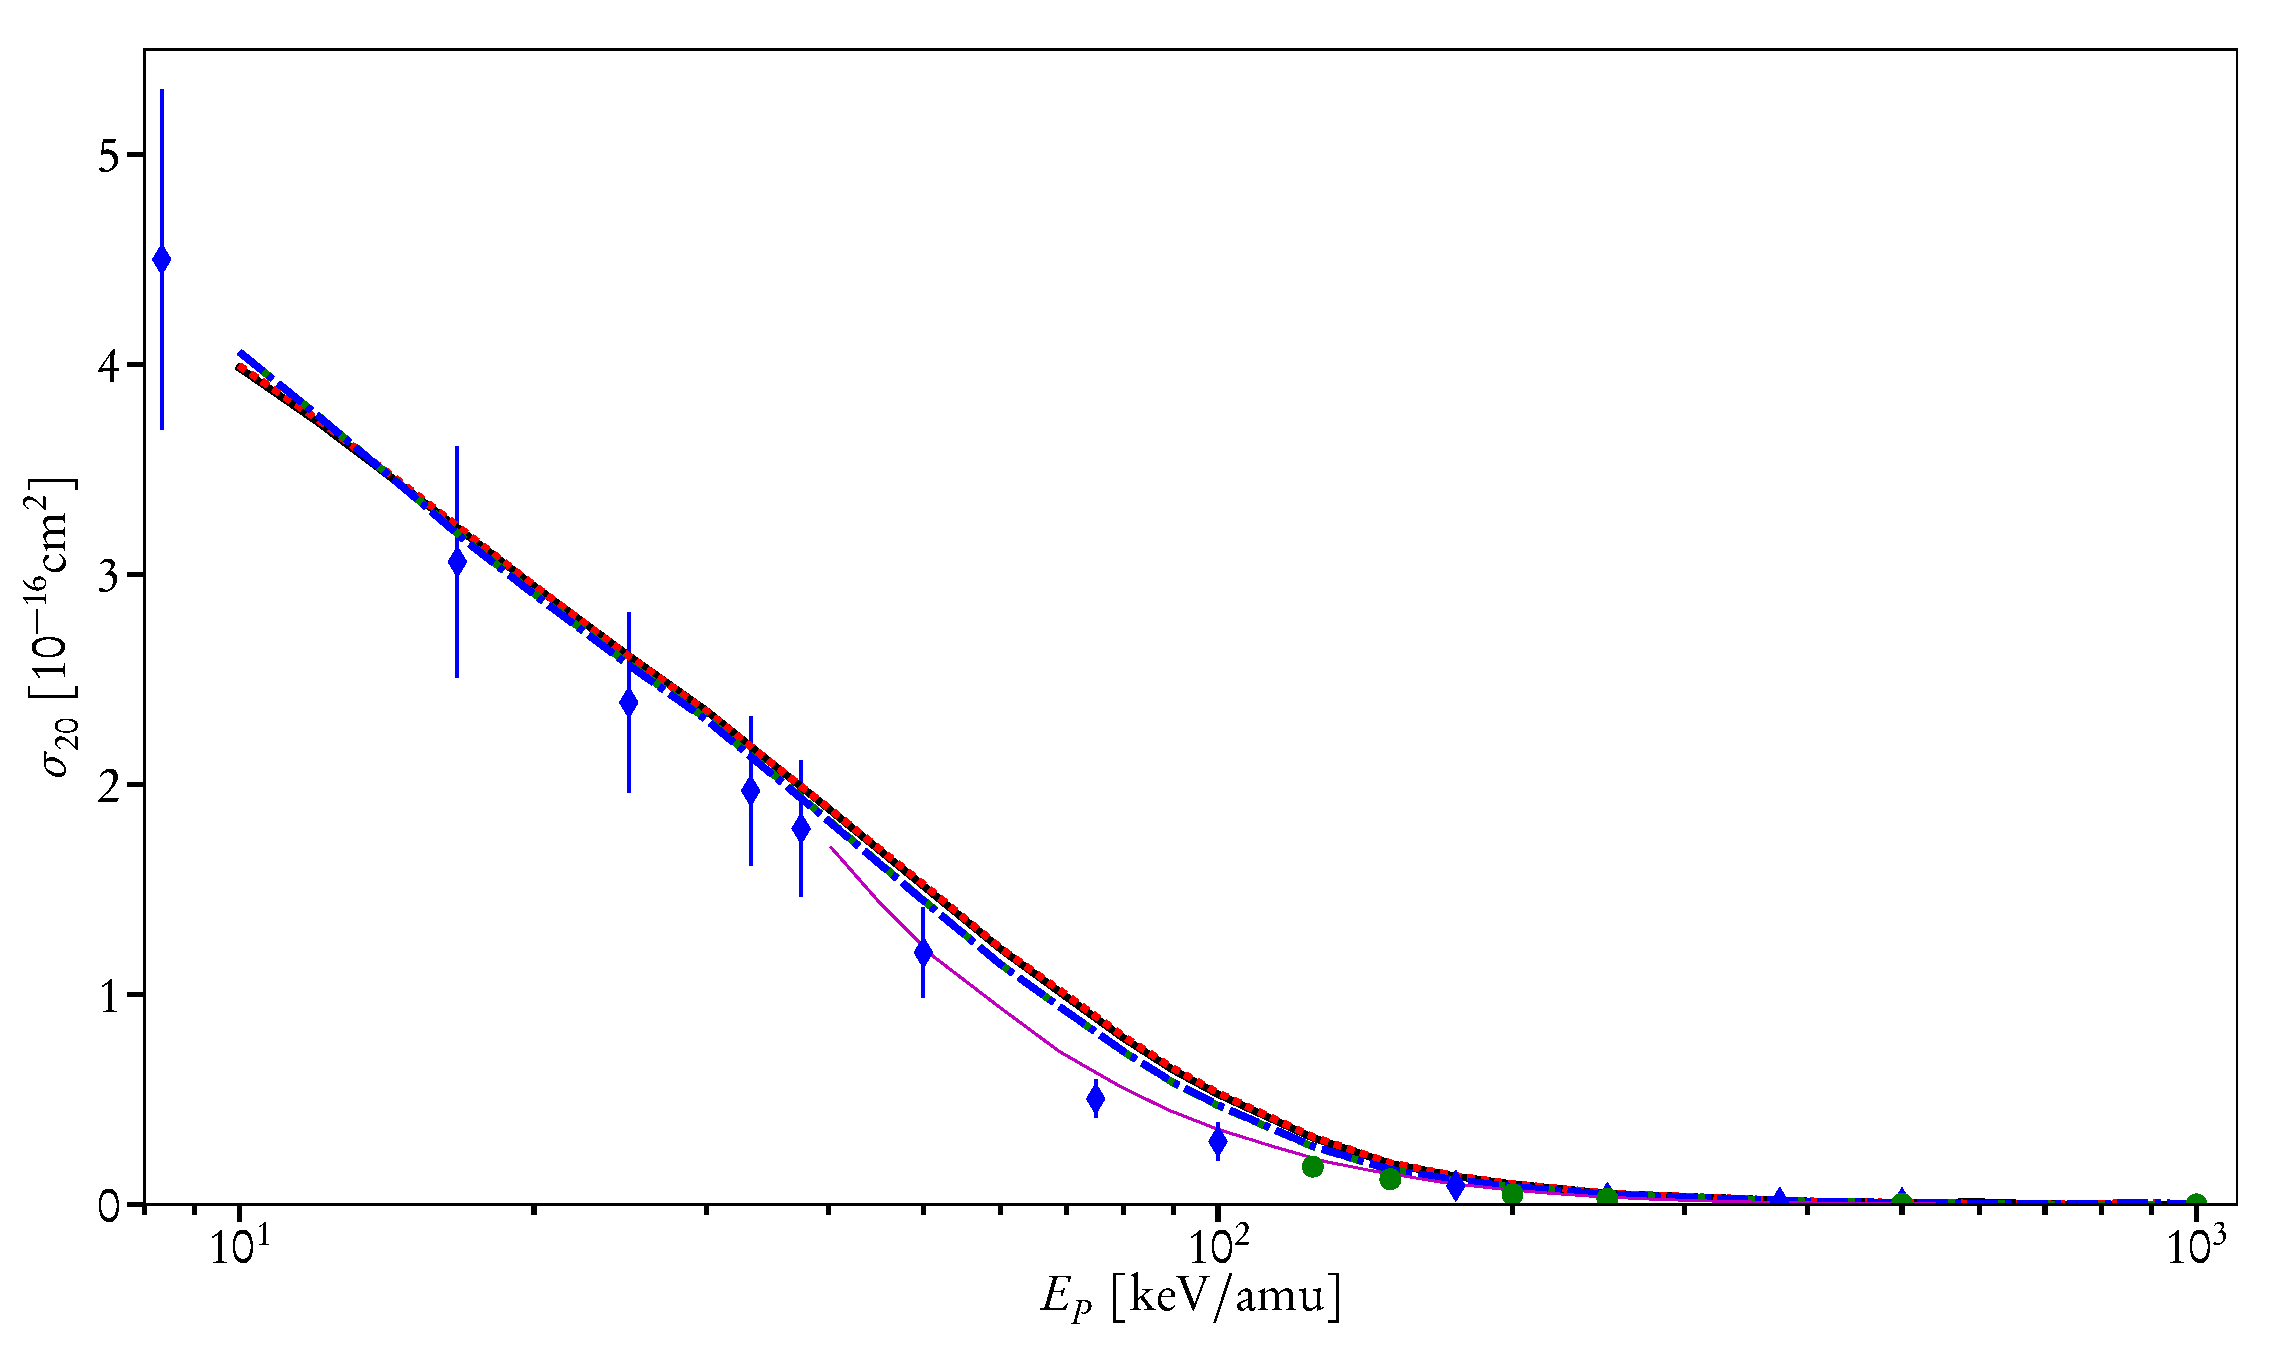
\includegraphics[width = \linewidth]{./images/hephe-cross/HepHe-120.eps}
            \caption[Total cross section for single capture to the projectile He\textsuperscript{+}-He
                     collisions.]
                    {Total cross section for single capture to the projectile.
                     Theoretical results: p\textsc{etf} response (solid line), n\textsc{etf} response
                                          (dotted line), p\textsc{etf} no-response (dashed line),
                                          n\textsc{etf} no-response (dash-dotted line), and
                                          \textsc{cdbw-4b} (post form) of Ghanbari-Adivi
                                          \textit{et al}.~\cite{GAG15} (dashed line).
                     Experimental data: diamonds~\cite{Dub-89} and circles~\cite{FTFHLP-95}.
                     \label{fig:cs120}}
         \end{figure}

         \begin{figure}[t]
            \centering
            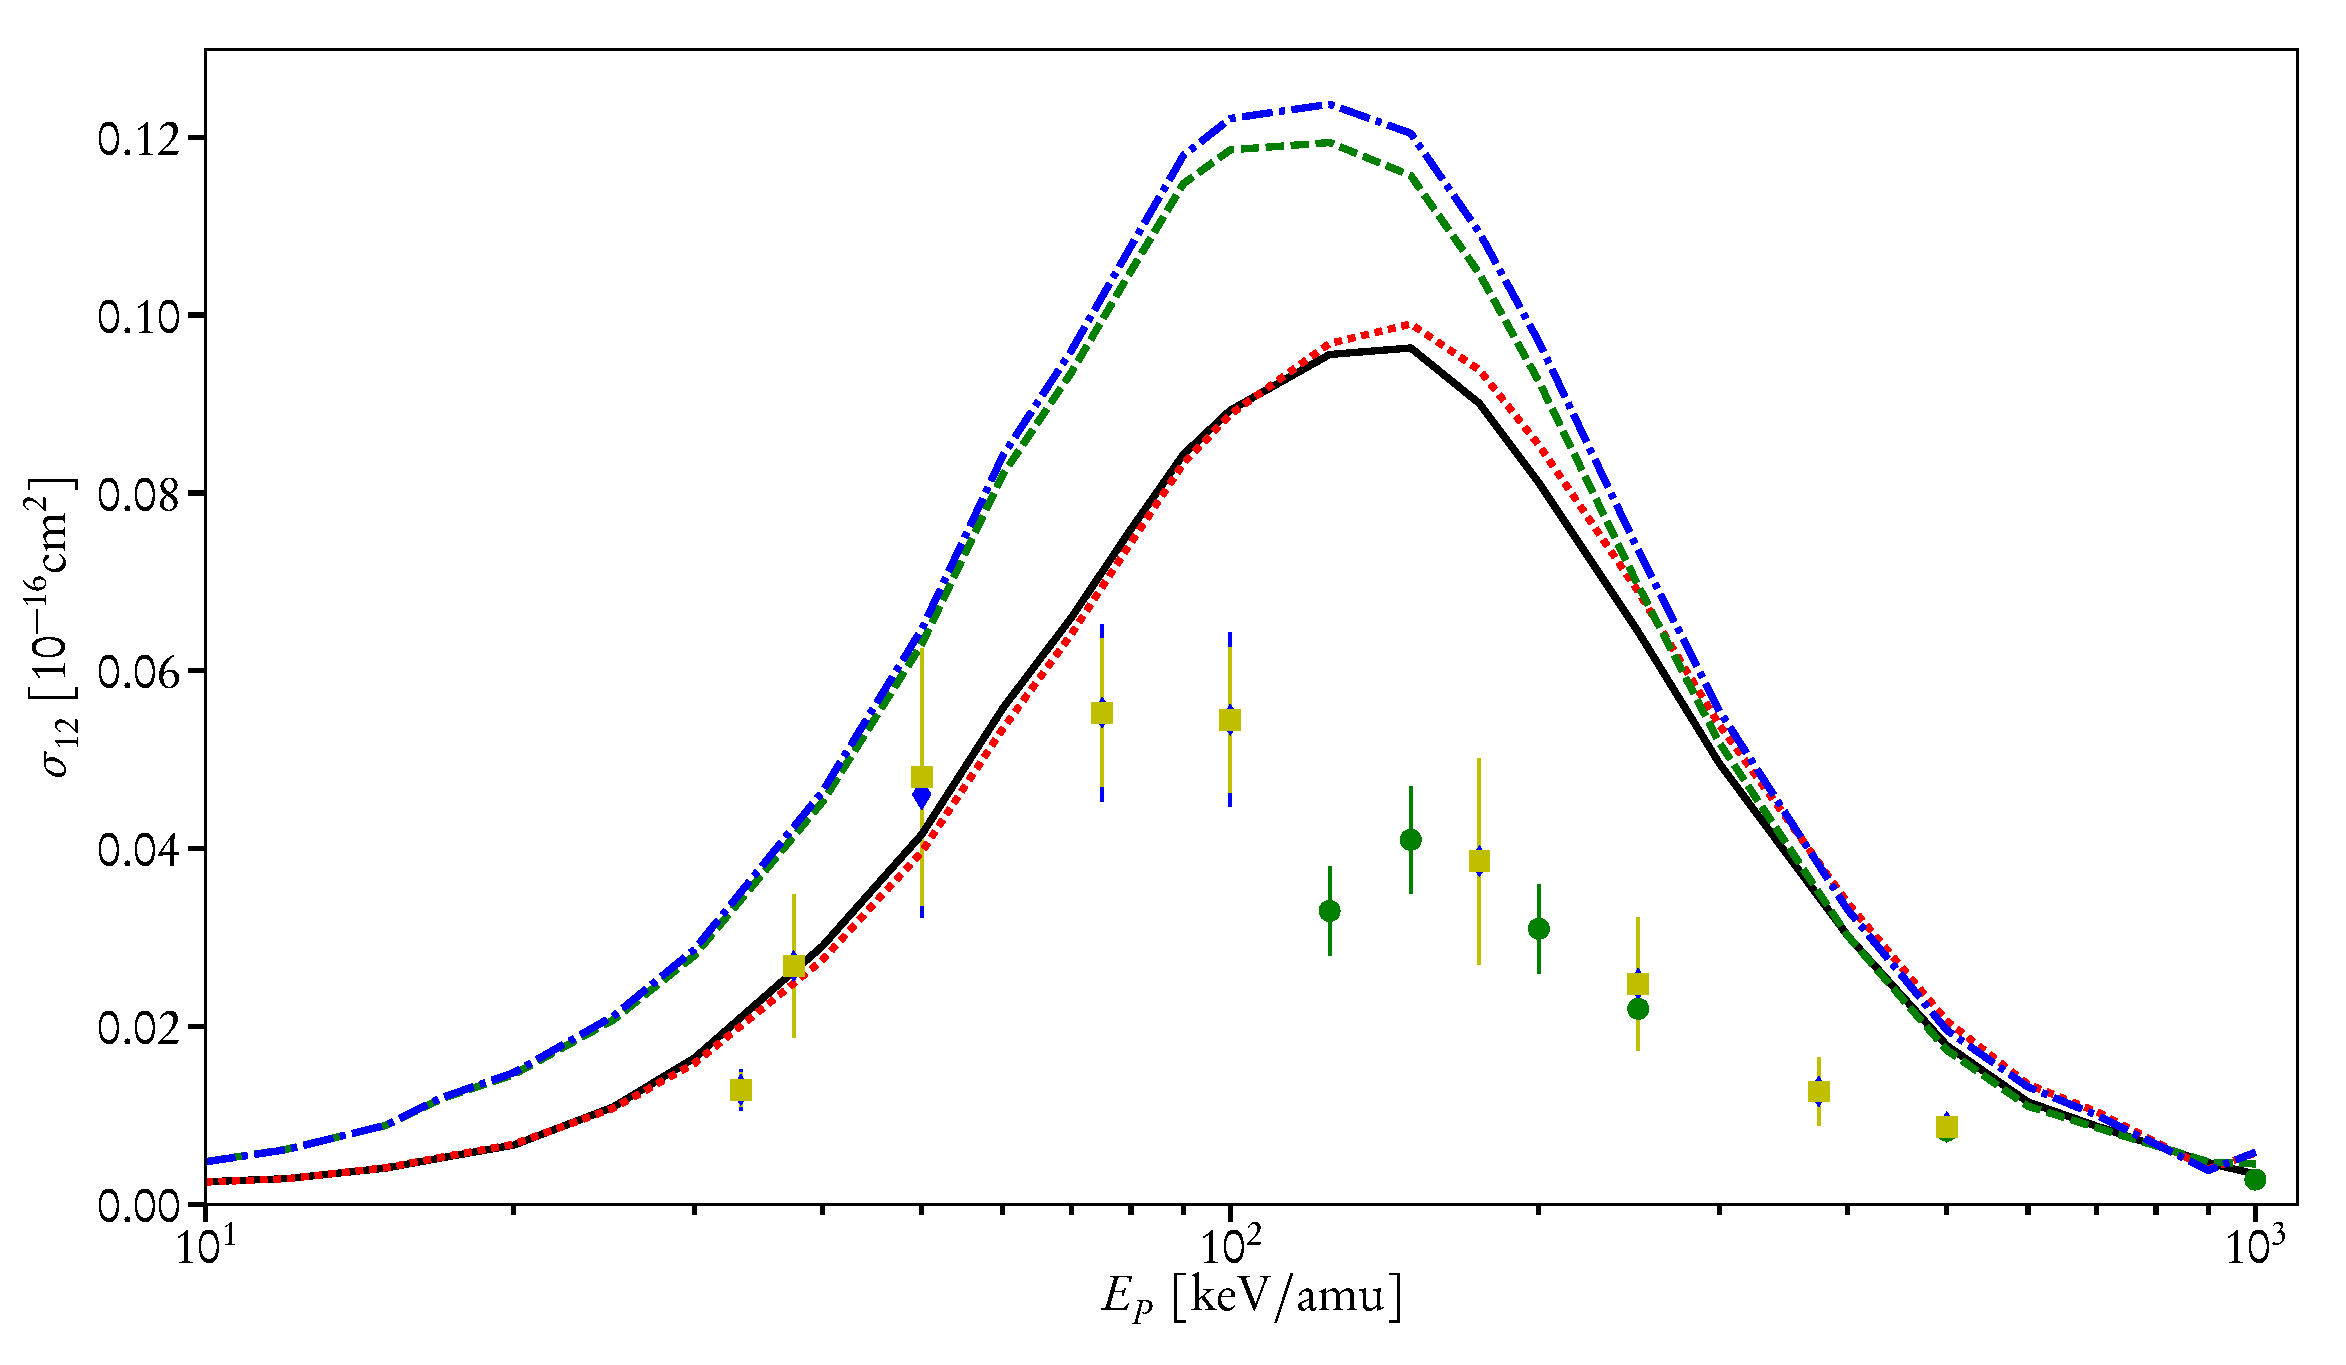
\includegraphics[width = \linewidth]{./images/hephe-cross/HepHe-012.eps}
            \caption[Total cross section for double ionization of the target in He\textsuperscript{+}-He
                     collisions.]
                    {Total cross section for double ionization of the target.
                     Theoretical results: p\textsc{etf} response (solid line), n\textsc{etf} response
                                          (dotted line). p\textsc{etf} no-response (dashed line), and
                                          n\textsc{etf} no-response (dash-dotted line).
                     Experimental data: diamonds~\cite{Dub-89}, circles~\cite{FTFHLP-95}, and
                                        squares~\cite{DT-88}. \label{fig:cs012}}
         \end{figure}

         \begin{figure}[t]
            \centering
            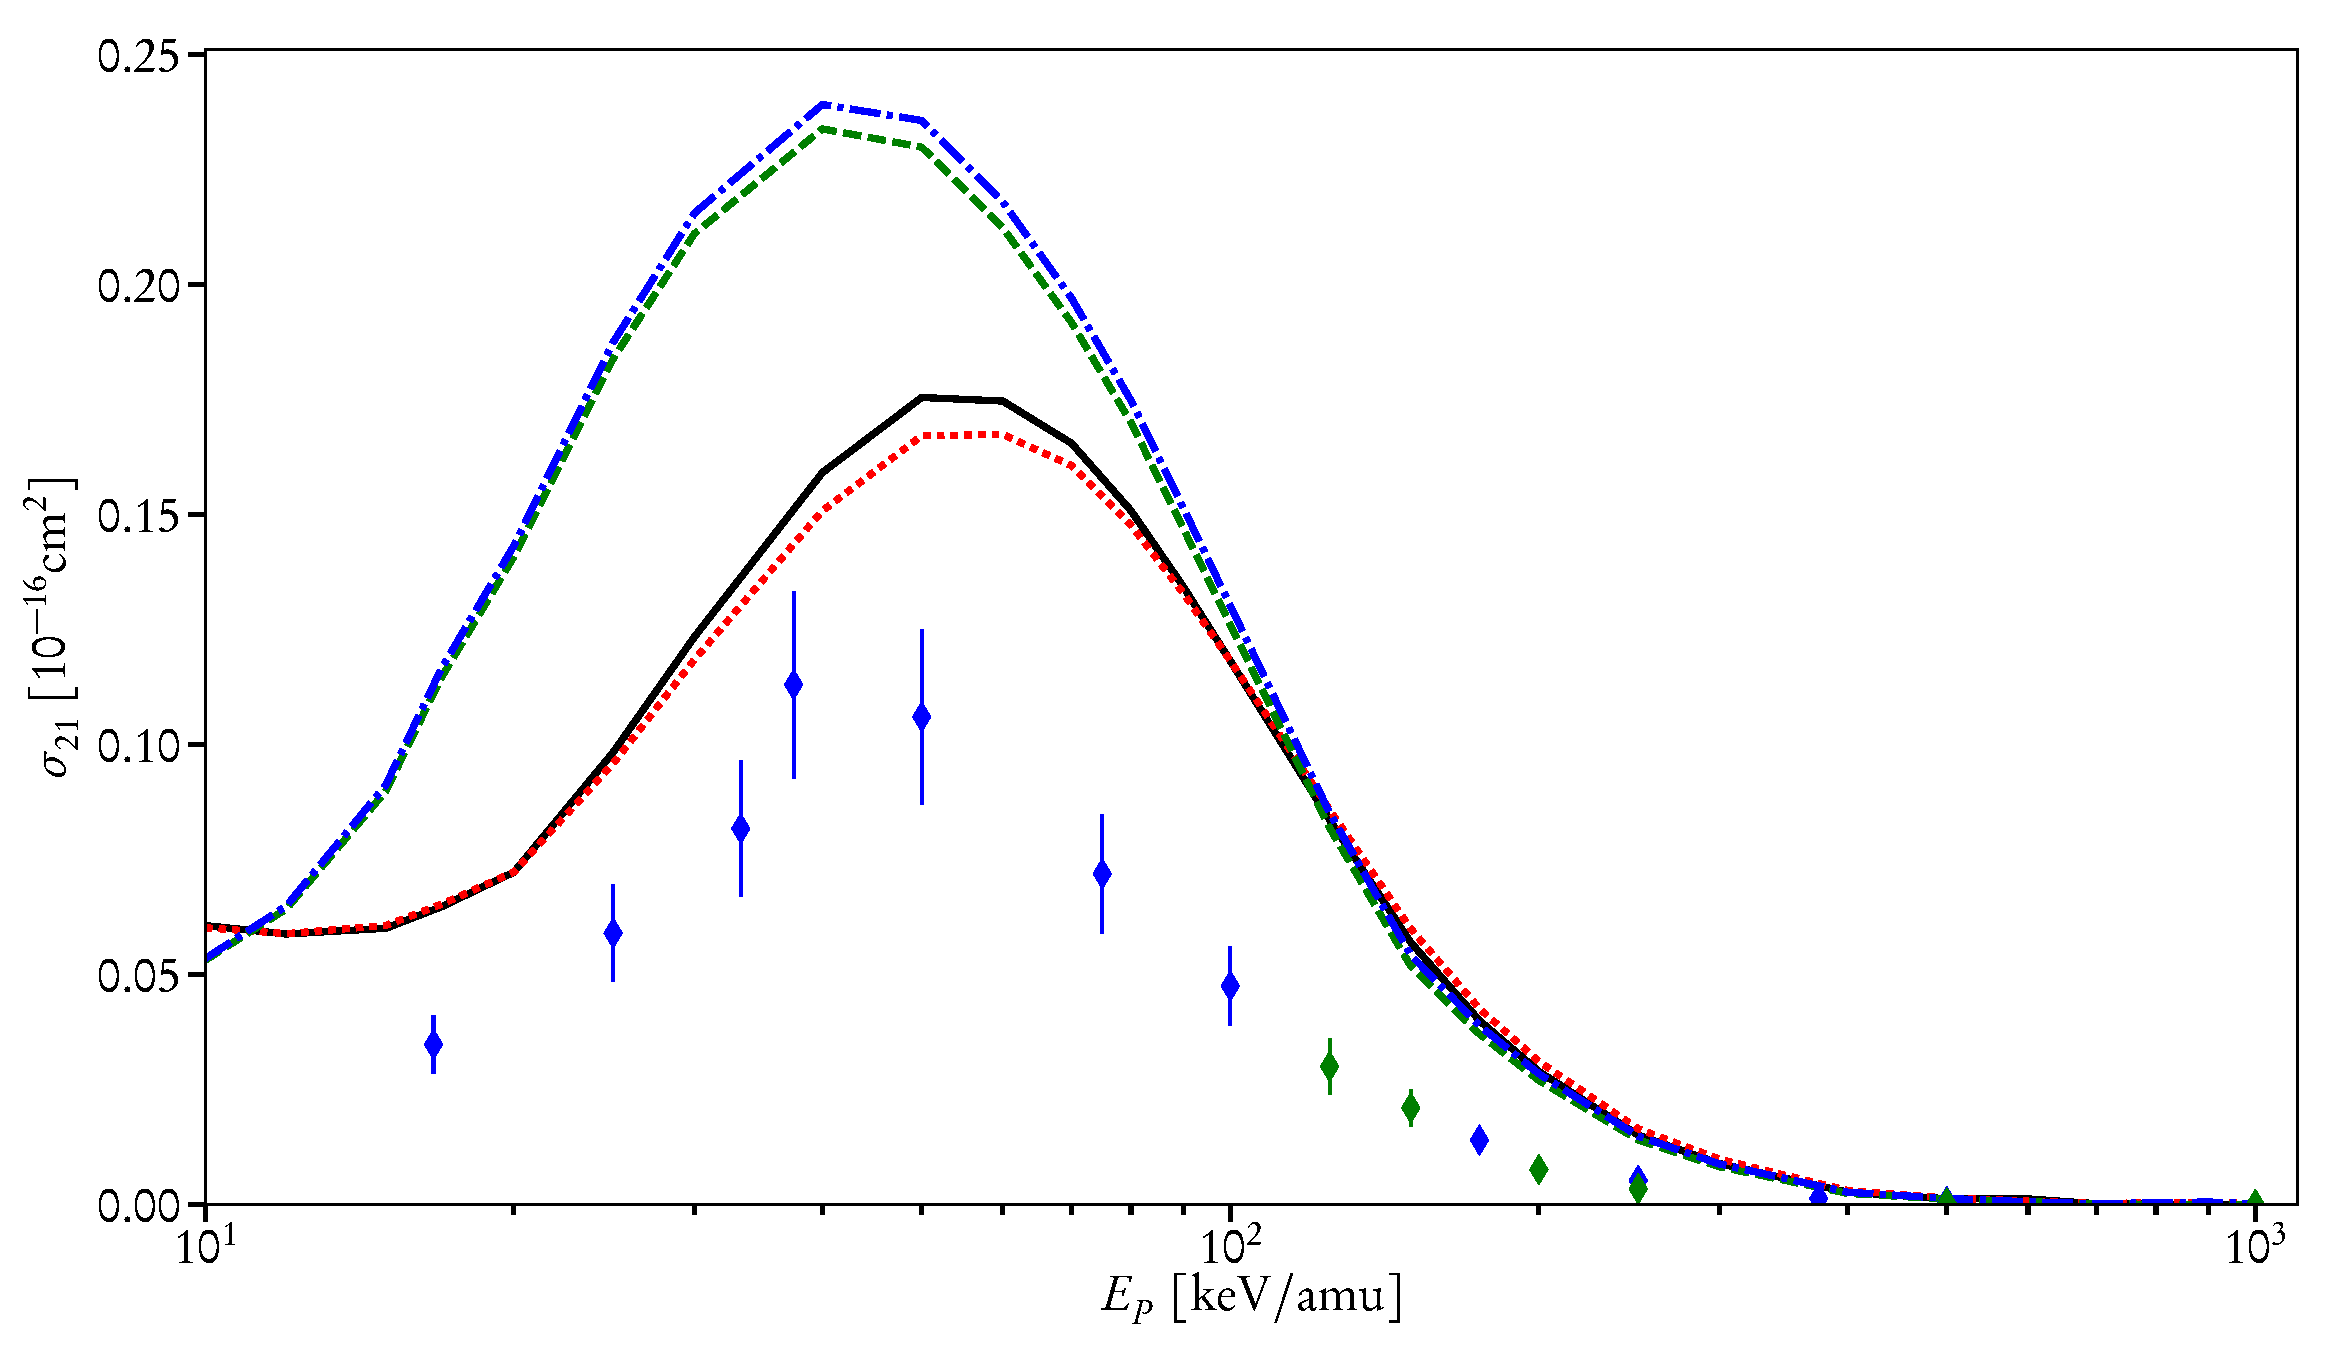
\includegraphics[width = \linewidth]{./images/hephe-cross/HepHe-021.eps}
            \caption[Total cross section for transfer ionization of the target in
                     He\textsuperscript{+}-He collisions.]
                     {Total cross section for transfer ionization of the target.
                     Theoretical results: p\textsc{etf} response (solid line), n\textsc{etf} response
                                          (dotted line), p\textsc{etf} no-response (dashed line), and
                                          n\textsc{etf} no-response (dash-dotted line).
                     Experimental data: diamonds~\cite{Dub-89} and circles~\cite{FTFHLP-95}.
                     \label{fig:cs021}}
         \end{figure}

         \begin{figure}[t]
            \centering
            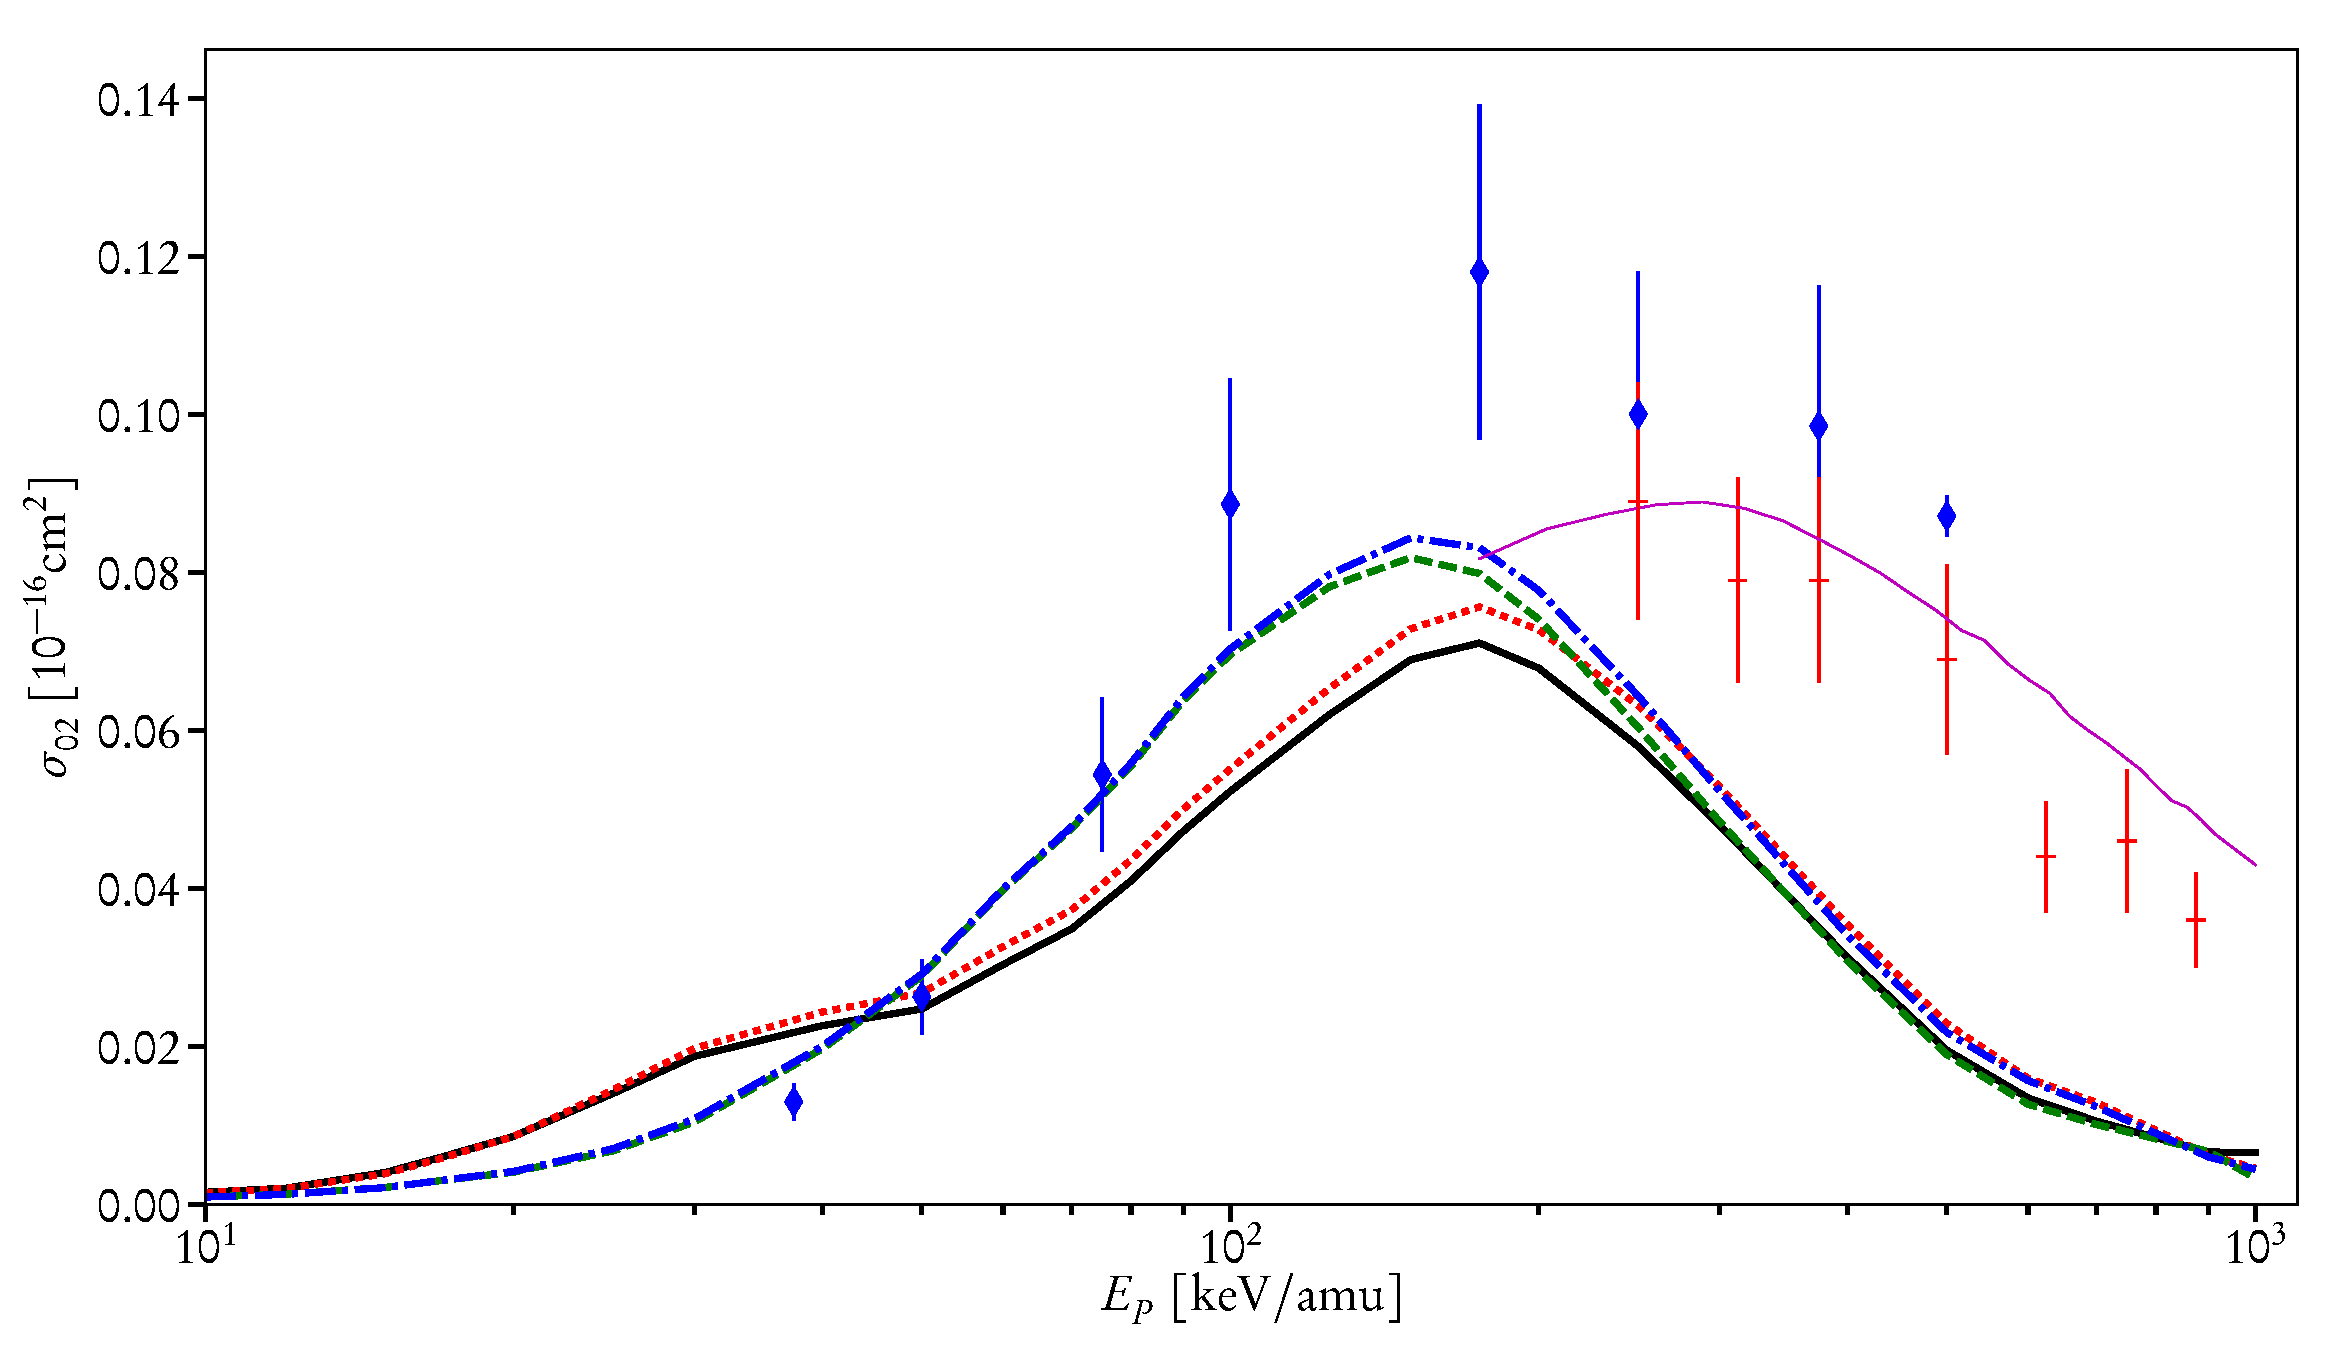
\includegraphics[width = \linewidth]{./images/hephe-cross/HepHe-102.eps}
            \caption[Total cross section for simultaneous single ionization of the target and projectile
                     in He\textsuperscript{+}-He collisions.]
                    {Total cross section for simultaneous single ionization of the target and
                     projectile.
                     Theoretical results: p\textsc{etf} response (solid line), n\textsc{etf} response
                                          (dotted line), p\textsc{etf} no-response (dashed line),
                                          n\textsc{etf} no-response (dash-dotted line), and
                                          \textsc{ievm} of Sigaud and Montenegro~\cite{SM-03} (thin
                                          solid line).
                     Experimental data: diamonds~\cite{Dub-89} and crosses~\cite{SSMSM-11}.
                     \label{fig:cs102}}
         \end{figure}

         \begin{figure}[t]
            \centering
            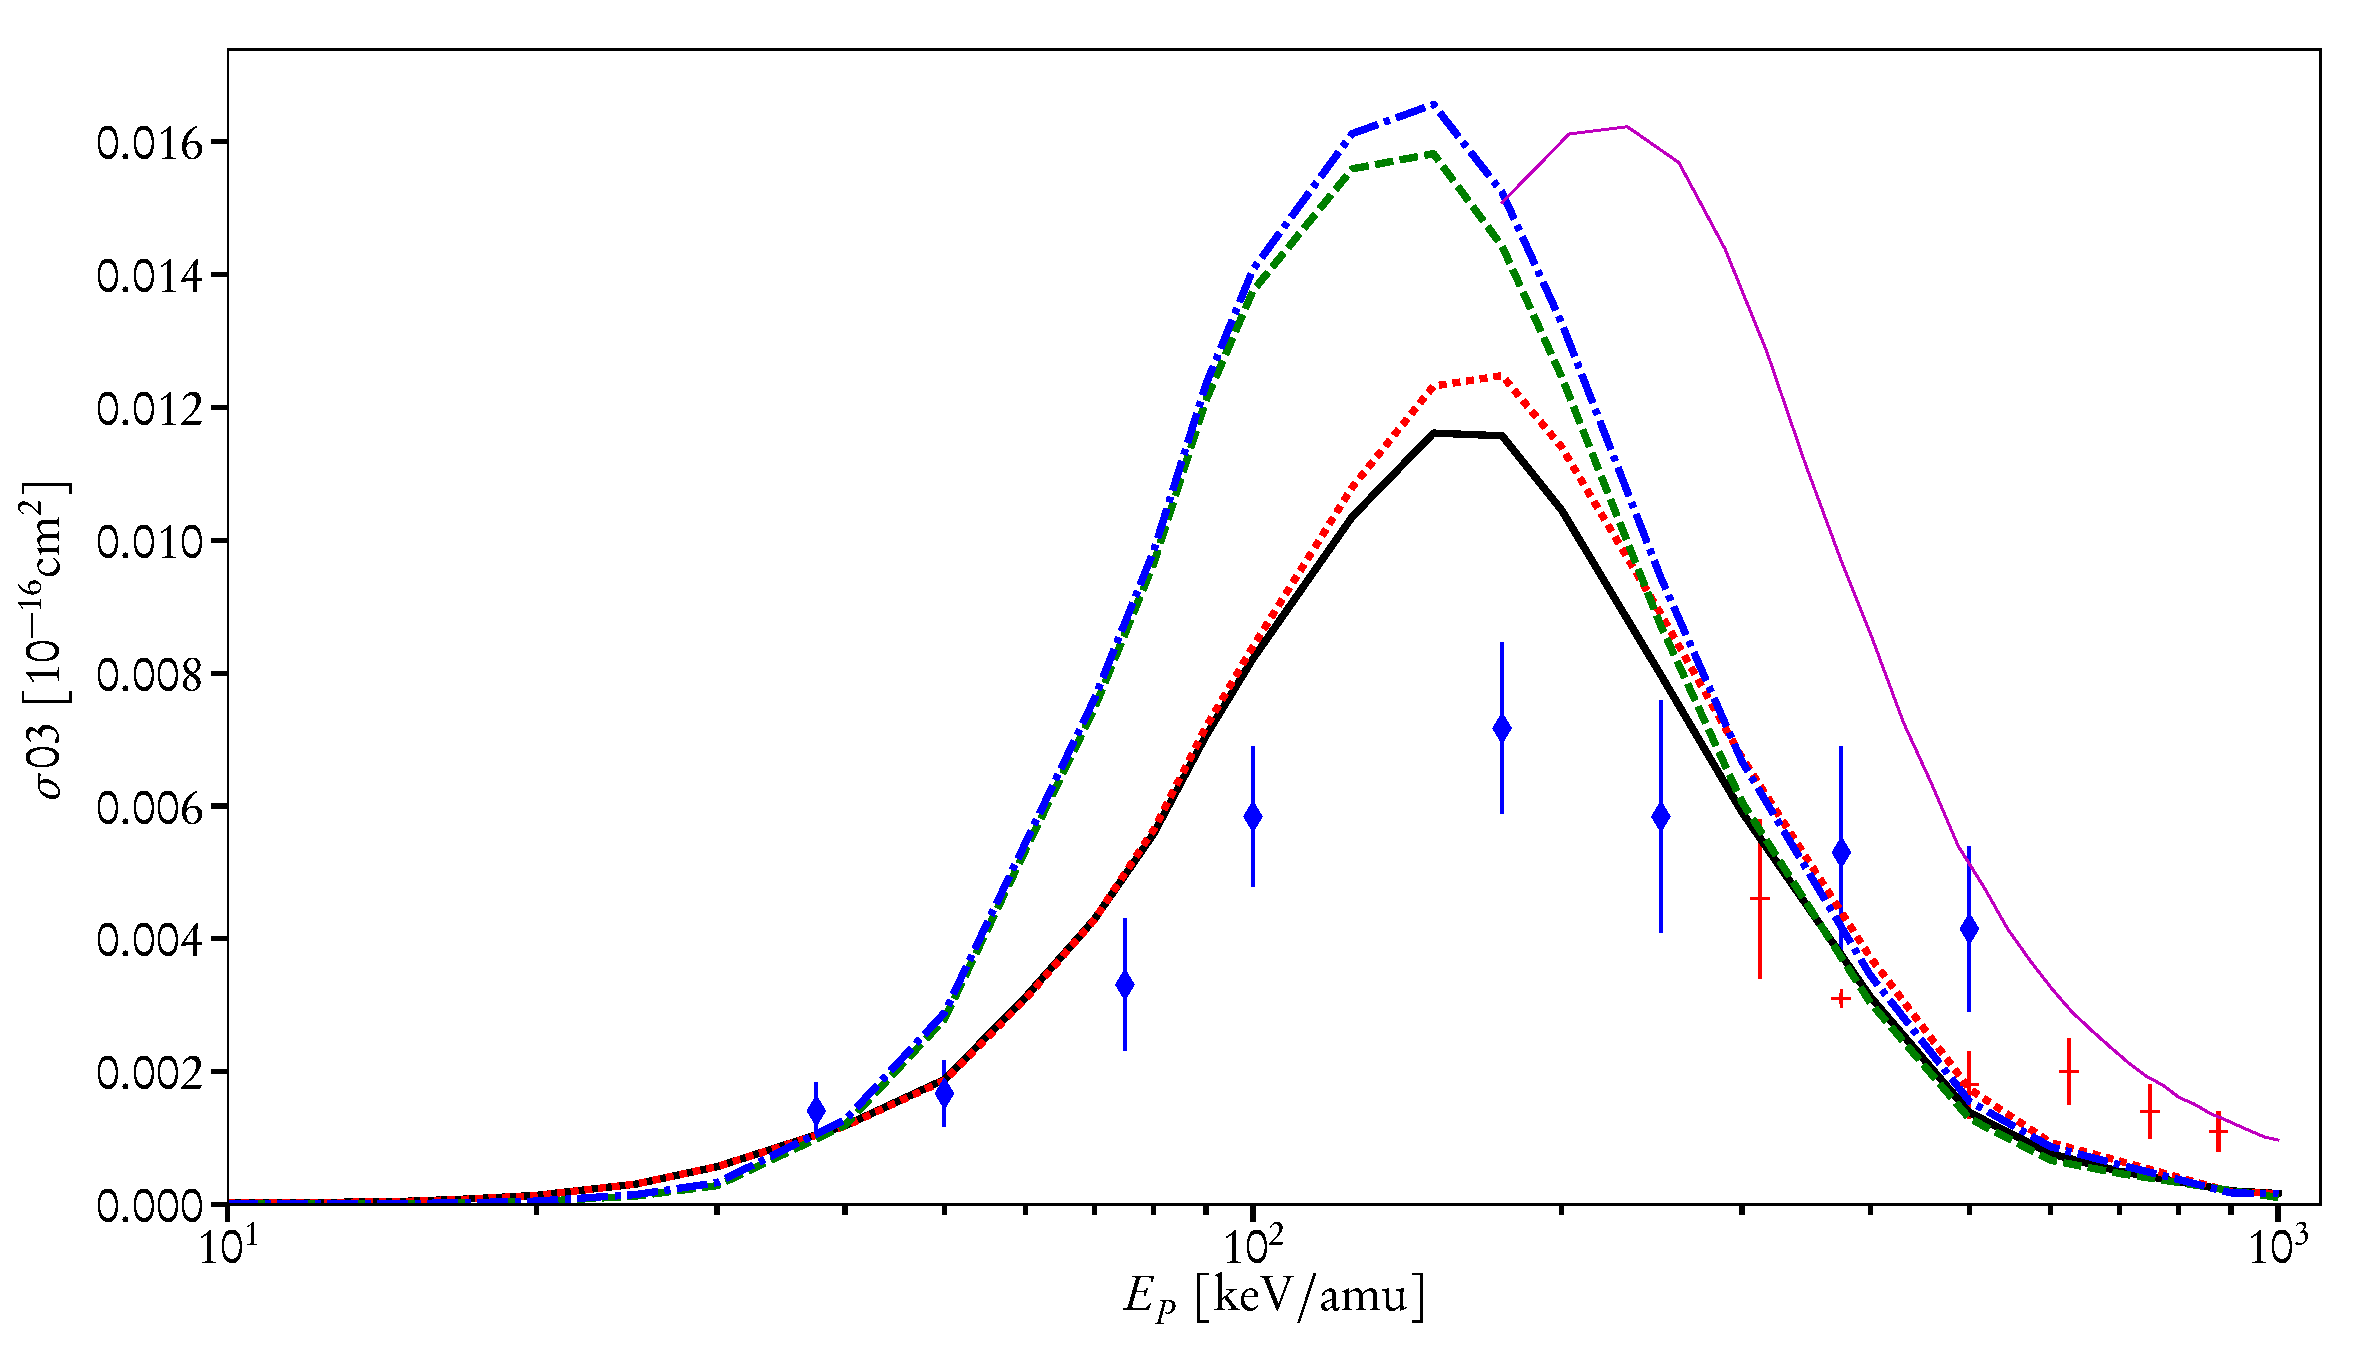
\includegraphics[width = \linewidth]{./images/hephe-cross/HepHe-003.eps}
            \caption[Total cross section simultaneous double target and single projectile ionization in
                     He\textsuperscript{+}-He collisions.]
                    {Total cross section simultaneous double target and single projectile ionization.
                     Theoretical results: p\textsc{etf} response (solid line), n\textsc{etf} response
                                          (dotted line), p\textsc{etf} no-response (dashed line),
                                          n\textsc{etf} no-response (dash-dotted line), and
                                          \textsc{ievm} of Sigaud and Montenegro~\cite{SM-03} (thin
                                          solid line).
                     Experimental data: diamonds~\cite{Dub-89} and crosses~\cite{SSMSM-11}.
                     \label{fig:cs003}}
         \end{figure}

         \begin{figure}[t]
            \begin{minipage}{.49\linewidth}
               \centering
               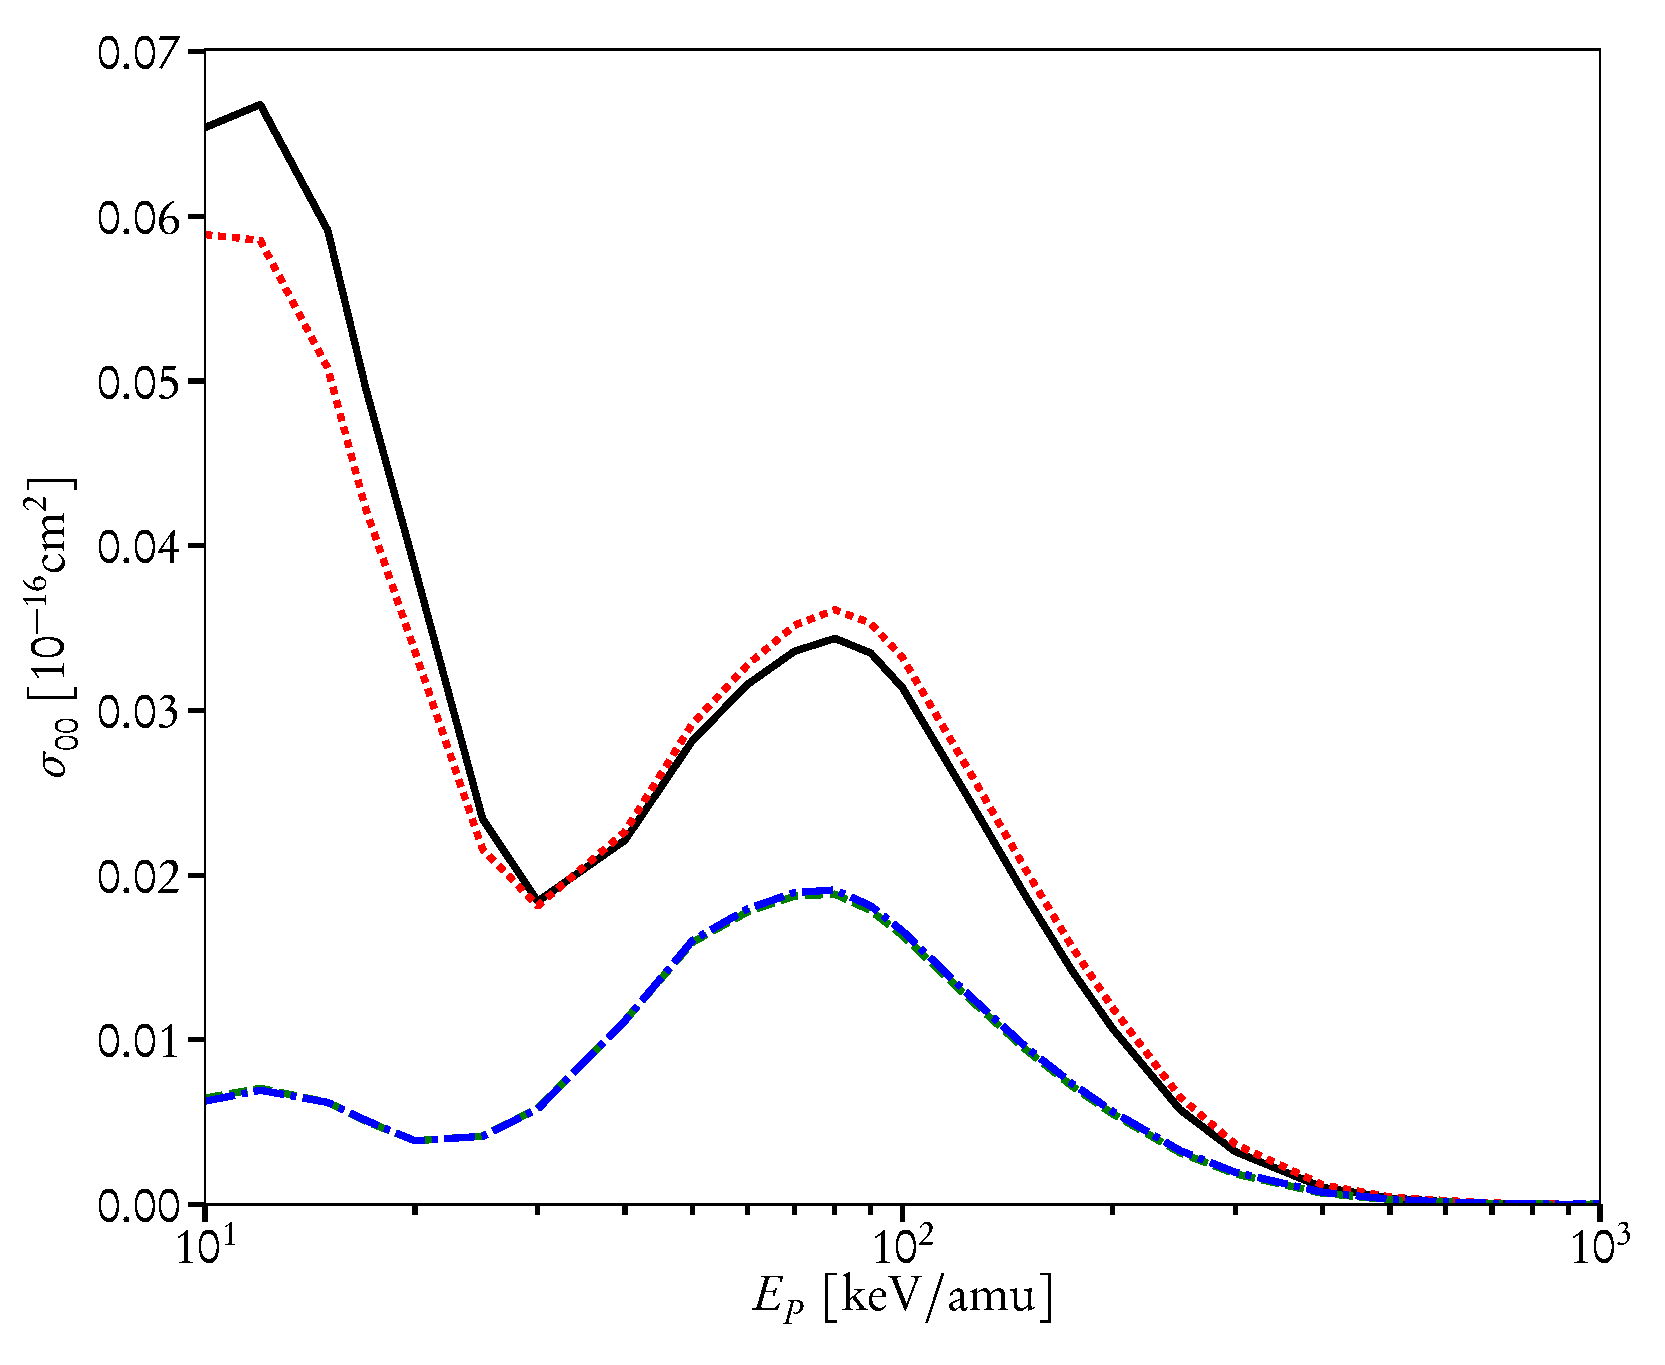
\includegraphics[width = \linewidth]{./images/hephe-cross/HepHe-300.eps}
               \caption[Total cross section for capture to the target in He\textsuperscript{+}-He
                        collisions.]
                       {Total cross section for capture to the target in He\textsuperscript{+}-He
                        collisions.
                        Theoretical results: p\textsc{etf} response (solid line), n\textsc{etf} response
                                             (dotted line), p\textsc{etf} no-response (dashed line), and
                                             n\textsc{etf} no-response (dash-dotted line).
                        \label{fig:cs300}}
            \end{minipage} \hspace{0.009\linewidth} %
            \begin{minipage}{.49\linewidth}
               \centering
               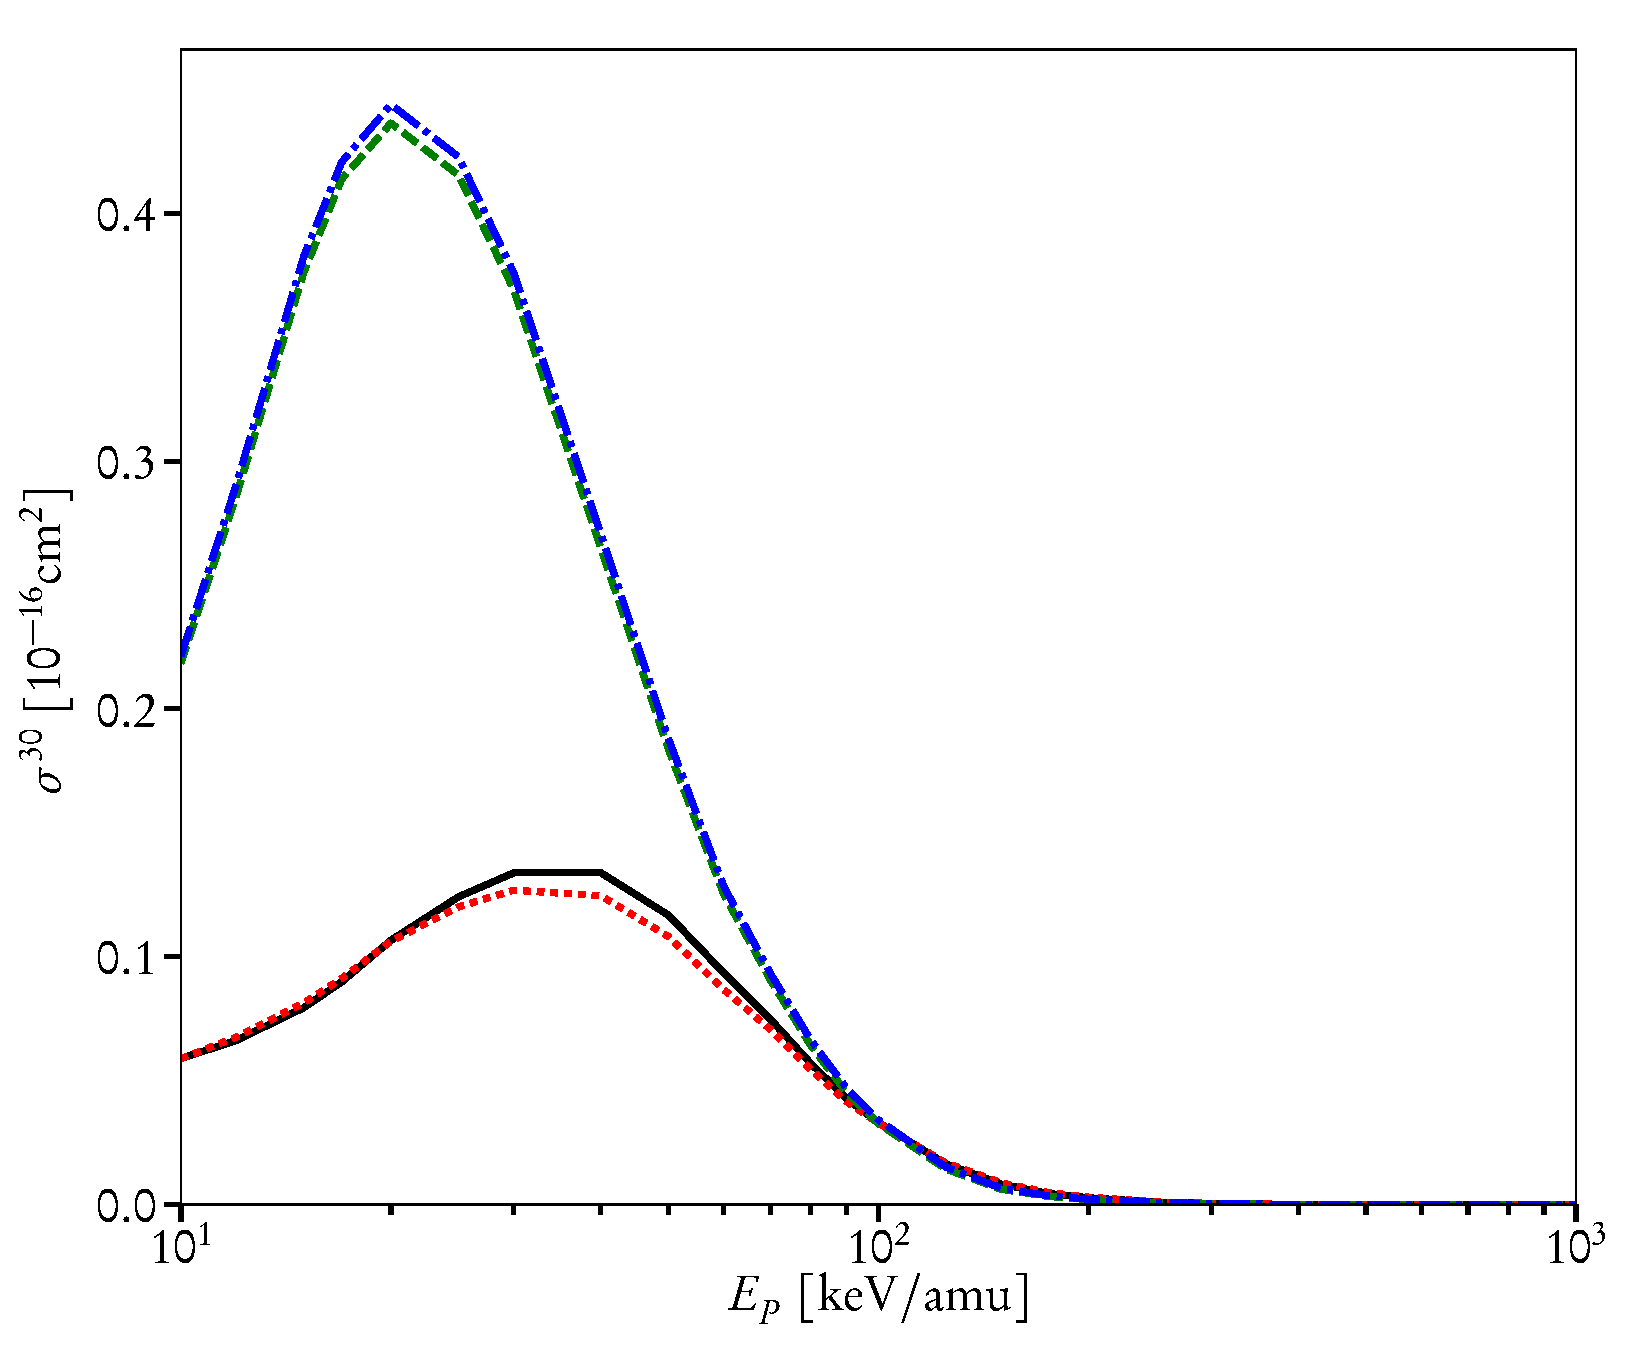
\includegraphics[width = \linewidth]{./images/hephe-cross/HepHe-030.eps}
               \caption[Total cross section for double capture to the projectile in
                        He\textsuperscript{+}-He]
                       {Total cross section for double capture to the projectile in
                        He\textsuperscript{+}-He.
                        Theoretical results: p\textsc{etf} response (solid line), n\textsc{etf} response
                                             (dotted line), p\textsc{etf} no-response (dashed line), and
                                             n\textsc{etf} no-response (dash-dotted line).
                        \label{fig:cs030}}
            \end{minipage}
         \end{figure}

         \begin{figure}[t]
            \centering
            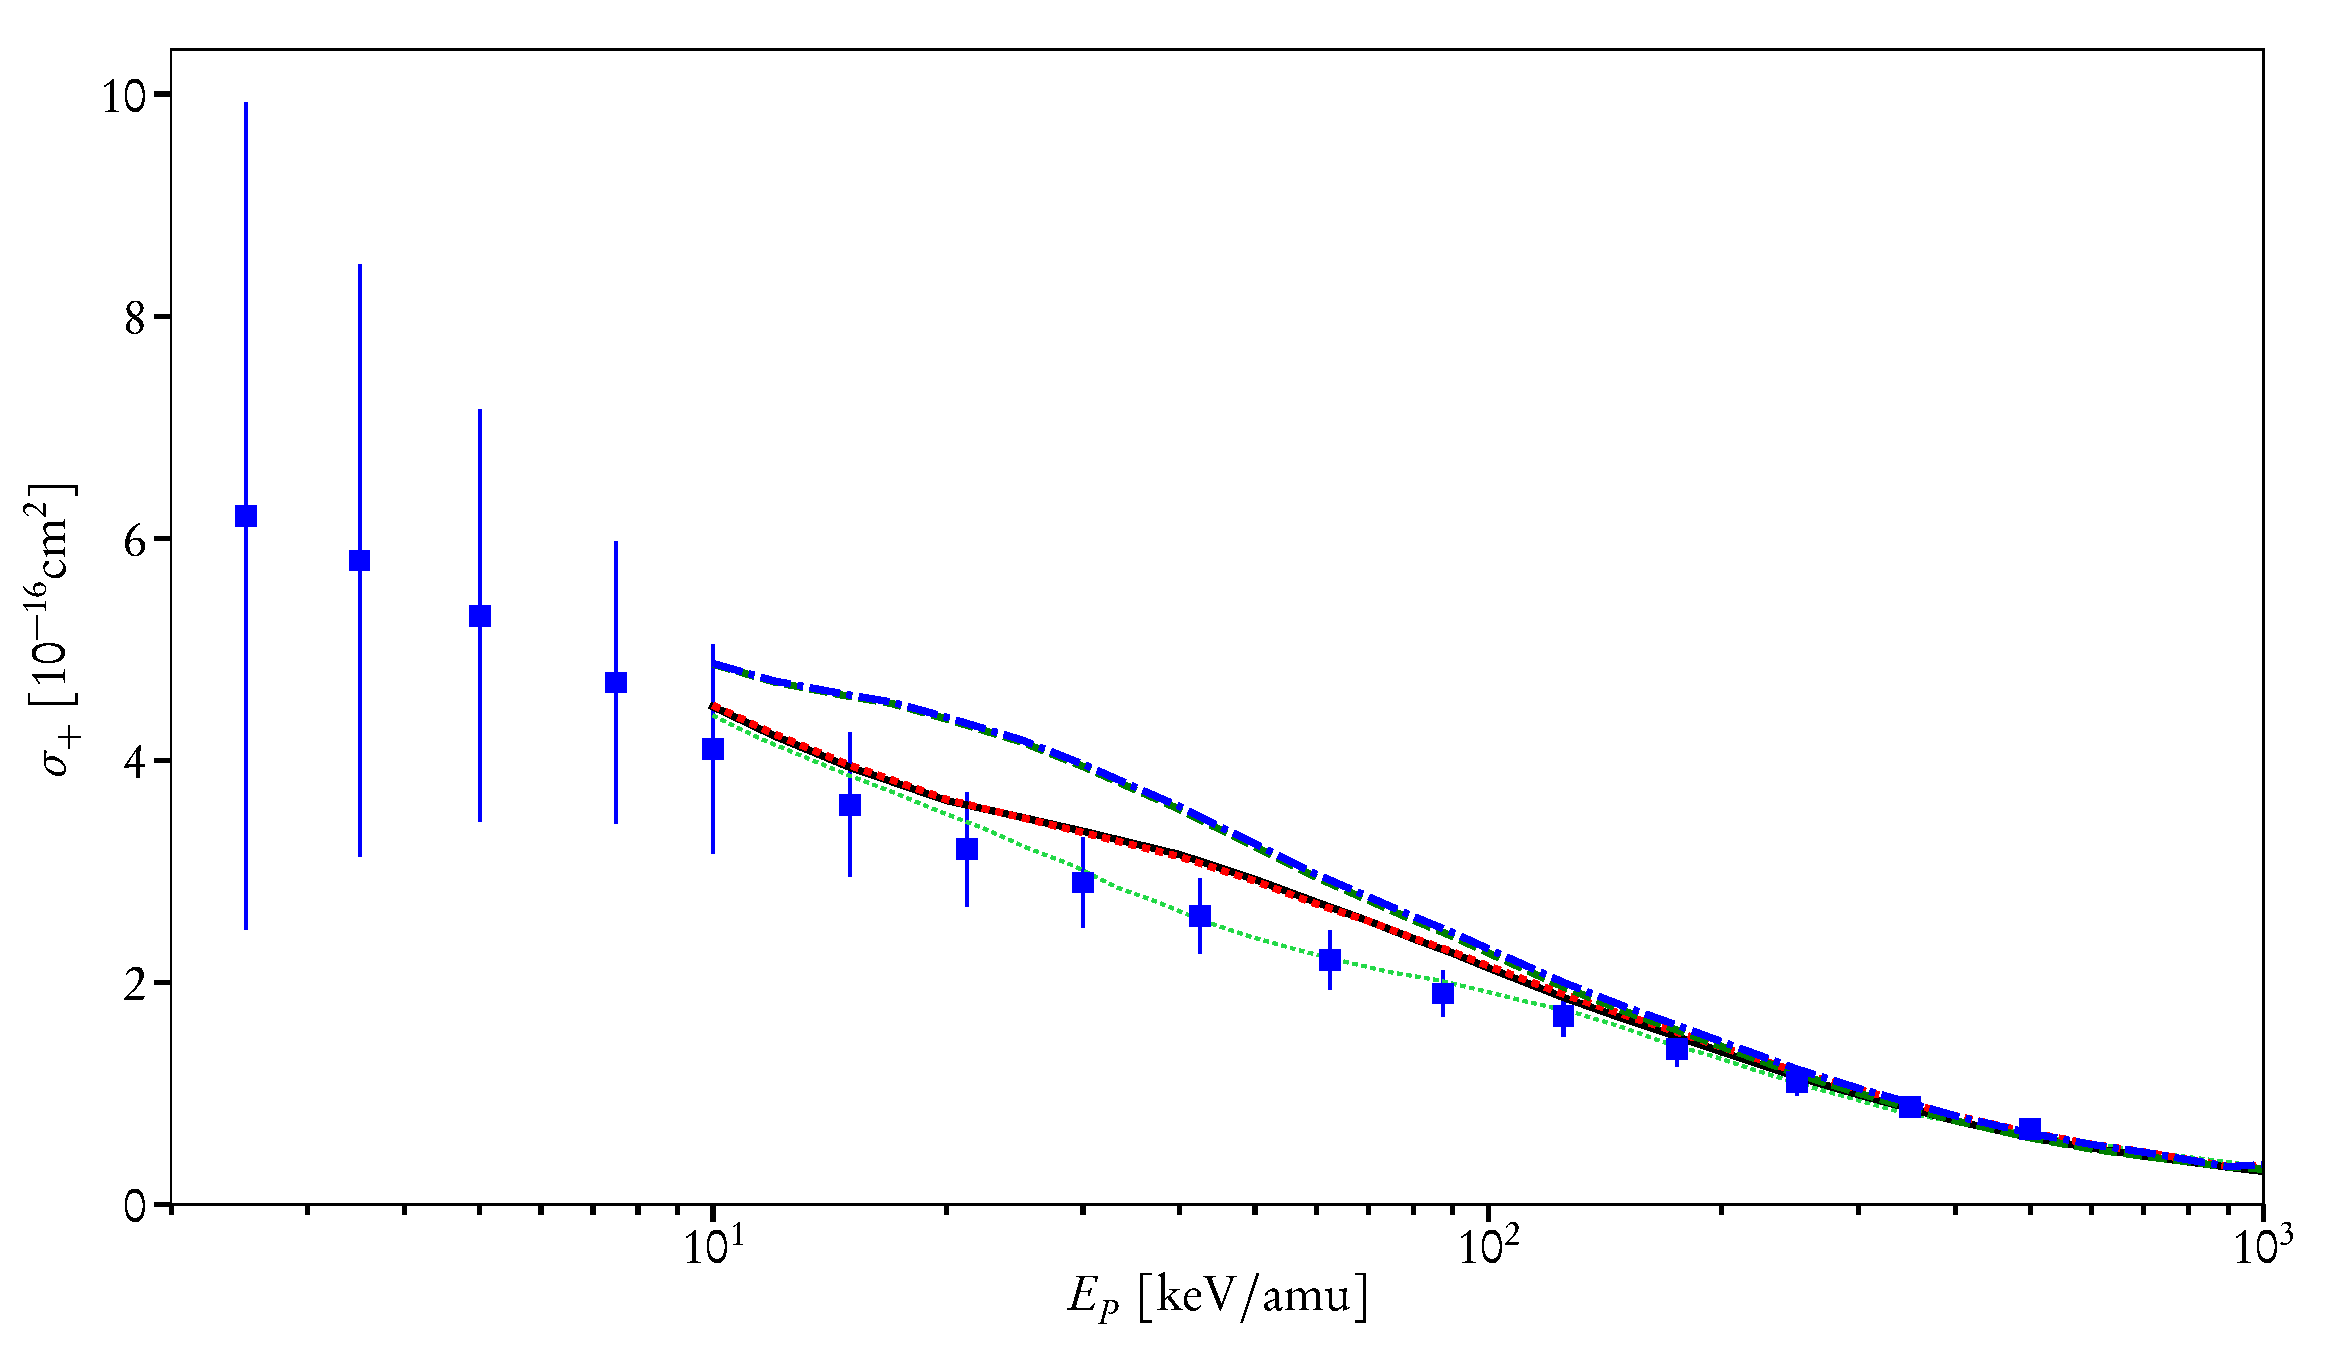
\includegraphics[width = \linewidth]{./images/hephe-cross/netRecoil.eps}
            \caption[Total cross section for net recoil ion production in He\textsuperscript{+}-He
                     collisions.]
                    {Total cross section for net recoil ion production in He\textsuperscript{+}-He
                     collisions.
                     Theoretical results: p\textsc{etf} response (solid line), n\textsc{etf} response
                                          (dotted line), p\textsc{etf} no-response (dashed line),
                                          n\textsc{etf} no-response (dash-dotted line), and
                                          \textsc{cmf} of Schenk~\cite{geraldDiss}
                                          (thin dotted line).
                     Experimental data: squares~\cite{RGID85}. \label{fig:recoil}}
         \end{figure}

         We now discuss the comparison of our response results with experimental data and other
         calculations by considering the single target ionization process of Eq.~\eqref{eq:tpi111}. The
         results for this channel, $\sigma_{11}$ are presented in Fig.~\ref{fig:cs111}. Both
         n\textsc{etf} and p\textsc{etf} are in good agreement with experiment throughout the full range
         of impact energies. The slightly lower values for the p\textsc{etf} version above 200~keV/amu
         make it a better fit to experiment. The underestimation of both curves below the peak
         corresponds almost exactly with the region where $\sigma_{20}$ results begin to rise above the
         experimental results (see Fig.~\ref{fig:cs120}).

         Also displayed in Fig.~\ref{fig:cs111} are the continuum-distorted-wave eikonal-initial-state
         approximation (\textsc{cdw-eis}) results of Miraglia and Gravielle~\cite{MG-10}. These results
         seem to compliment the results of the present work through the majority of the impact energy
         range. One notable exception to this is the slightly higher cross section maximum however. As
         there is a fairly large spread in the experimental data around this region it is difficult to
         say which is more accurate. The results of Miraglia and Gravielle also begin to diverge as one
         approaches lower impact energies. This feature is likely due in large part to the perturbative
         nature of \textsc{cdw-eis} which becomes less reliable as one decreases the impact energy.

         Next, we consider the results for $\sigma_{01}$ [Eq.~\eqref{eq:tpi201}] shown in
         Fig.~\ref{fig:cs201}. As with the previous channel both n\textsc{etf} and p\textsc{etf} results
         are in reasonable agreement with the experiment where it is available. Also following the
         general trend described above both models begin essentially equal at low impact energies and
         separate as $E_P$ increases. Both models begin to over estimate the data above the peak around
         200~keV/amu. Once again the slightly lower p\textsc{etf} results are in better agreement with
         experiment. The slight unphysical structures in the curves below 40~keV/amu seem to correspond
         with the peaks of the $\sigma_{00}$ channel. This issue will be discussed in greater detail
         below.

         These calculations have been compared with the independent event model (\textsc{ievm}) results
         of Sigaud and Montenegro~\cite{SM-03}. While they do not directly report $\sigma_{01}$ they do
         present $\sigma_{02}$, $\sigma_{03}$, and what they call total electron loss (we will denote
         this by $\sigma_\mathrm{total}$). Using the relation
         %
         \begin{equation} \label{eq:total}
            \sigma_\mathrm{total} = \sigma_{01} + \sigma_{02} + \sigma_{03}
         \end{equation}
         %
         one can easily determine $\sigma_{01}$ from their disclosed results. Their values seem to be in
         much better agreement with experiment in the high energy range than either n\textsc{etf} or
         p\textsc{etf} models. This can perhaps be explained by the presence of correlation in the
         \textsc{ievm} calculations. As will be discussed in more detail below all of our models
         underestimate $\sigma_{02}$ and $\sigma_{03}$ in this impact energy range. Keeping in mind that
         $\sum p_{kl} = 1$ the increase in these channels resulting from the incorporation of
         correlation effects, so-called antiscreening in particular, would be drawn in part from the
         current channel of focus $\sigma_{01}$ resulting in a decrease putting our results in better
         agreement with both Sigaud and Montenegro and the experimental data.

         For the results of single electron capture to the projectile, the process of
         Eq.~\eqref{eq:tpi120} depicted in Fig.~\ref{fig:cs120}, both n\textsc{etf} and p\textsc{etf}
         models are essential identical. This is what one would hope for as they are in good agreement
         with experiment in the entire range of impact energies. A possible explanation of the slight
         discrepancy between theory and experiment in the 50-150~keV/amu interval is offered by a
         comparison with the four-body Coulomb–Born distorted wave approximation (\textsc{cdbw-4b})
         results of Ghanbari-Adivi \textit{et al}.~\cite{GAG15}. The correlation effects included in
         this model may point to the slight rise in cross section being related to the fact that we have
         employed an \textsc{iem} approximation. Alternatively, the rise may be due to a failure of the
         partial \textsc{etf}.

         The latter explanation may provide a more satisfying solution to this problem. One would expect
         that capture processes should be dominated by the contributions of slow and close collisions.
         The regions where the n/p\textsc{etf} models start to diverge from experiment is approximately
         the region where both models begin to diverge in other channels (see for example $\sigma_{12}$
         in Fig.~\ref{fig:cs012}), that is the lowest energies where \textsc{etf}s are important.
         Additionally they begin to agree with experiment once the cross sections begin to rapidly
         approach zero, for fast collisions. This would seem to be an indication that correct
         \textsc{etf}s are important for capture processes (a fact that should be at least intuitively
         obvious).

         A few words should be spent addressing the choice for the theoretical calculation compared
         against. Unlike other channels there exists a relatively large number of works to select from
         that fit the criteria listed above. As the majority of these belong to a family of related
         perturbative models~\cite{Mancev96, BOC05, Mancev-07, MG-10, NTC11, GG-12b, GAG15} the latest,
         that of Ghanbari-Adivi \textit{et al}., was chosen. A comparison of the work of Ghanbari-Adivi
         \textit{et al}.\ with several earlier perturbative calculations can be found in
         Ref.~\cite{GAG15}.

         With the single-electron processes taken care of double target ionization,
         Eq.~\eqref{eq:tpi012}, the first of the two-electron processes will be considered next. The
         results for this channel are presented in Fig.~\ref{fig:cs012}. As with previous channels both
         n\textsc{etf} and p\textsc{etf} results appear to be very similar with a slight edge going to
         the p\textsc{etf} model's marginally lower results above 100~keV/amu. Both models seem to shift
         the peak in the cross section to higher impact energy than experiment would suggest is correct.
         As one would expect from an \textsc{iem} the two models exaggerate double ionization, see for
         example Refs.~\cite{pbarhe-rev, p-he2p-he}. As there are no previous works fitting the
         conditions for inclusion listed earlier little else can be concluded about the results of the
         present work.

         Another channel where the literature lacks a proper touchstone is that of transfer ionization
         [Eq.~\eqref{eq:tpi021} shown in Fig.~\ref{fig:cs021}]. The trends for $\sigma_{21}$ are very
         similar to those of $\sigma_{12}$. As with the previously discussed process both models are
         above experiment and shift the experimental peak to a higher impact energy. The only
         significant difference is that this is one of the few channels where the n\textsc{etf} model
         tends to give larger cross section values and is in slightly better agreement with experiment
         than the p\textsc{etf}. The flattening of the curves below 20~keV/amu is an artifact of the
         \textsc{tc-bgm} becoming less reliable at the lowest impact energies.

         The last two-electron process is simultaneous single ionization of the target and projectile,
         Eq.~\eqref{eq:tpi102}. The results for our n\textsc{etf} and p\textsc{etf} models are presented
         in Fig.~\ref{fig:cs102}. These results both follow the trend of the data quite closely,
         arguably matching the position of the peak in the experimental cross sections. This channel is
         the second of two where the n\textsc{etf} model has a slight egde over the results of the
         p\textsc{etf}. Unfortunately they fall below experiment for the majority of the impact energy
         range shown.

         A comparison with the \textsc{ievm} of Sigaud and Montenegro explains this fact. Sigaud and
         Montenegro claim to capture the effects of antiscreening, the direct interaction between target
         and projectile electrons, which becomes increasingly important for projectile ionization
         processes at larger impact energies. As the results of the current work are those of an
         \textsc{iem} they make no effort to capture any correlation effects. Sigaud and Montenegro's
         efforts to capture antiscreening see their results fall within experiment for their entire
         extent. Encouragingly, if one were to extend the curve of Sigaud and Montenegro it would seem
         to overlap with the results of the present work lending credence to the curve in the region
         below the cross section peak, where antiscreening cannot contribute.

         Next wee will consider the sole three electron process, simultaneous double target and single
         projectile ionization [Eq.~\eqref{eq:tpi003}]. The results, presented in Fig.~\ref{fig:cs003},
         again follow the general trends found in the previously discussed channels; overestimation of
         the cross section peak and a slightly better showing for the p\textsc{etf} model over the
         results of the n\textsc{etf} model. Unlike for previous channels our results are in better
         agreement with experiment than those of Sigaud and Montenegro which over estimate the cross
         sections to a greater extent and over a larger impact energy range. As in previous channels the
         under estimation of our cross sections at larger impact energies may be attributed to
         correlation effects, in particular, to antiscreening which  Sigaud and Montenegro seem to
         exaggerate in this channel.

         In addition to the outcome channels discussed above there are three further processes. One,
         $\sigma_{10}$, has been left out as it involves no charge transfer. The other two,
         $\sigma_{00}$ and $\sigma_{30}$, involve all three electrons bound to either the target or the
         projectile and are displayed in Figs.~\ref{fig:cs300} and \ref{fig:cs030}. As was pointed out
         earlier these channels should not be considered due to the fact that the production cross
         sections for these configurations should be negligible, unfortunately in our results they are
         not. While modelling the initial and final states of the system as single Slater determinants
         accounts for Pauli exclusion which precludes all three electrons from occupying the ground
         state there is nothing in the model to stop additional electrons from capturing and remaining
         in excited states. Keeping in mind that this model is simply an example of an \textsc{IEM},
         albeit a sophisticated one, the probabilities for these unphysical channels will behave in a
         predictable manner $p_{00} \sim {p_T}^3$ and $p_{30} \sim {p_P}^3$. The inclusion of functional
         correlation should, in principle, provide an offset. An exaggerated example of this is
         provided in Chap.~\ref{chap:p-he2p-he} where a \textsc{wb} type model could potentially cause
         both channels to be zero. The only recourse, short of implementing a model which contains at
         least some functional correlation, is to artificially redistribute the probability from
         $p_{00}$ and $p_{30}$ into other channels.

         Two options immediately present themselves. The first possibility is to feed the extra
         probability into the corresponding ionization channels. In other words, $p_{00}$ and $p_{30}$
         would augment $p_{01}$ and $p_{21}$ respectively. With the peak in $\sigma_{30}$ approximately
         matching that of $\sigma_{21}$ in both position and magnitude this solution would lead to a
         doubling of the over estimation present in the $\sigma_{21}$ channel. A similar issue would
         arise in the lower impact energy range of the $\sigma_{01}$ curve. This leaves one with the
         second option, to put the extra probability from $p_{00}$ into $p_{10}$ and feed $p_{30}$ into
         $p_{20}$. The only effect this could have on the presented results would be to increase
         $\sigma_{20}$ however, as $\sigma_{30}$ is at worst an order of magnitude less than
         $\sigma_{20}$ it would provide only a small shift in the curve displayed in
         Fig.~\ref{fig:cs120}.

         To close out this section we will consider the total cross section for net recoil ion
         production. This quantity, presented in Fig.~\ref{fig:recoil}, may be calculated from
         previously presented results
         %
         \begin{equation}
            \sigma_{+} = \sigma_{11} + \sigma_{20} + \sigma_{02} + 2 \sigma_{12} + 2 \sigma_{21}
                                     + 2 \sigma_{03} + 2 \sigma_{30}.
         \end{equation}
         %
         Just as in the separate channels the response results are lower than those of the no-response
         model for the majority of the impact energy range putting them in fair agreement with
         experiment outside of the imtermediate energy range. No distinction between n\textsc{etf} and
         p\textsc{etf} curves is discernible.

         Also show in Fig.~\ref{fig:recoil} are the common mean field (\textsc{cmf}) results of Schenk
         and Kirchner~\cite{geraldDiss}. The \textsc{cmf} which is in good agreement with experiment.
         The difference between the \textsc{cmf} results and those of the current work can be traced to
         the overestimation of single capture (see discussion above and Fig.~\ref{fig:cs120}). As was
         discussed in Ref.~\cite{geraldDiss} the \textsc{cmf} model is very well suited for describing
         processes involving initial target electrons. This in large part due to the fact that in the
         \textsc{cmf} both target and projectile electrons are propagated with the same Hamiltonian,
         that of the target. One can see this as evidence that the current work trades an excellent
         description of a single centre for a slightly less realistic description of both atomic
         centres.

      \end{subsection}

   \end{section}

\end{chapter}

\begin{chapter}{Conclusion \label{chap:con}}

   Following the programme laid out in the introduction this work has presented investigations of an
   increasingly complex series of ion-atom collisions systems. This journey began with the relatively
   simple antiproton-helium system, continued with the proton-helium and He\textsuperscript{2+}-He
   systems, and culminated in a discussion of the He\textsuperscript{+}-He collision system. In the
   proceeding subsections more detailed and collision specific conclusions will be offer for these
   investigations. Before embarking on a summary of individual results it is, perhaps, necessary to
   emphasize one of the overarching themes of this work. In most situations our results are competitive
   with the best models of others. In many cases our results are the only ones which can consistently
   describe all outcome channels for a given collision system, that is they produce some of the best
   results available without being focused on a specific process. This certainly demonstrates the
   utility of density functional theory techniques over a fairly wide range of systems.

   \begin{section}{\texorpdfstring{$p$}{p}-He and \texorpdfstring{He\textsuperscript{2+}}{He2+}-He
                   Collisions \label{sec:con-phe2p-he}}

      We have investigated correlation effects in $p$-He and He\textsuperscript{2+}-He collisions. By
      expanding the correlation integral model of Wilken and Bauer~\cite{wb} applied previously to the
      antiproton-helium system~\cite{pbarhe} we have produced total cross sections for single, double,
      and transfer ionization as well as single and double capture. In order to incorporate electron
      capture processes into the \textsc{wb} model two additional correlation integrals, one centred on
      the projectile ($I^{PP}_\mathrm{c}$) and the other two-centred ($I^{TP}_\mathrm{c}$), were
      introduced. While $I^{PP}_\mathrm{c}$ was dealt with using straight forward modification of the
      original \textsc{wb} model. $I^{TP}_\mathrm{c}$ was determined based on the values of the other
      correlation integrals and the single particle probabilities, $p_T$ and $p_P$. The use of this
      model was justified by the favourable $p$-He results for single capture that depend on only
      $I^{TP}_\mathrm{c}$ explicitly.

      For the majority of the channels investigated the \textsc{wb} model represents a clear improvement
      over \textsc{iem}  results, the most notable exceptions being the double ionization results at low
      and intermediate impact energies. Where enough correlated two-electron calculations exist to make
      a proper comparison these fully correlated calculations represent a much larger improvement over
      \textsc{iem} than \textsc{wb} results.

      Overall it appears that the $p$-He results are superior to those of the He\textsuperscript{2+}-He
      system. The variation in the quality of results may be attributed to the increased charge of the
      projectile. The stronger potential well on the projectile results in an increase in the role of
      capture in the dynamics. Immediately, this means that the problems present in all calculations of
      separating the target, capture, and ionizing regions becomes amplified. The increased role of
      capture also enters into the \textsc{wb} model itself where the previously closed $p_P > 1/2$
      branches of the correlation integrals are opened, further complicating the analysis. The lack of a
      full reference calculation over a wide impact energy range makes separating these issues all the
      more difficult.

      The opening of the capture channels introduces additional complications into the \textsc{wb}
      model. First, it accentuates some of the short comings of the underlying dynamic calculation.
      While some gains may be made by rerunning these calculations using the full \textsc{tc-bgm} the
      base level accuracy of the method is essentially fixed (especially at low impact energies). One
      could take this as more confirmation that no single calculation is yet capable of covering vast
      tracts of impact energy space~\cite{LRV-14}. In this regard our results cover more channels, over
      a larger energy range than most.

      Second, the \textsc{wb} model itself appears to distribute probabilities among the six outcome
      channels in unphysical ways (for example causing double and transfer ionization in $p$-He
      collisions to be equal). While the precise origin of these issues is not currently known at least
      some blame must be taken by the piece-wise nature of the adiabatic approximation which causes only
      one of $I^{TT}_\mathrm{c}$ or $I^{PP}_\mathrm{c}$ to be nontrivial at any given impact parameter.
      Another source of poor probability partitioning is the model chosen for $I^{TP}_\mathrm{c}$ which,
      as mentioned above, causes $p_{II} = p_{IP}$. Regardless of the provenance of these issues further
      applications of the \textsc{wb} model in the context of capture are inadvisable. This should,
      however, not be interpreted as a criticism of correlation-integral models in general merely a
      reflection of the \textsc{wb} model's apparent limitations. Work in this vein can be made easier
      provided more correlated two-electron calculations become available.

   \end{section}

   \begin{section}{\texorpdfstring{He\textsuperscript{+}}{He+}-He Collisions \label{sec:con-hephe}}

      The He\textsuperscript{+}-He collision system was investigated within  time-dependent spin-density
      functional theory under the constraints of the exchange-only approximation. An accurate
      time-dependent exchange potential was determined through the application of the \textsc{kli}
      approximation. Total cross section results for all physical outcome channels were then offered in
      the approximate impact energy of range 10-1000~keV/amu for two models; one in which electron
      translation factors were ignored and a second model where partial \textsc{etf}s
      were used. The results of both models are in overall good agreement with experiment.

      Without diminishing the results of this work it is necessary to highlight a few limitations and
      where the results may be improved in future iterations. First, the restriction of the
      implementation of the \textsc{kli} functional to systems of cylindrical symmetry is the impetus
      for both the 1s-only approximation as well as the need to consider both the n\textsc{etf} and
      p\textsc{etf} models. Future applications of the procedure laid out in this work would benefit
      greatly from a fully three-dimensional implementation of the \textsc{kli} functional that makes no
      symmetry assumptions. Failing this, it may be possible to express the \textsc{ks} orbitals in
      terms of a multipole expansion. In this way more complex, symmetry respecting orbitals may be
      obtained.

      Comparisons of our results with the theoretical works of other groups points to the fact that the
      calculations would also gain from the inclusion of correlation effects. Treating this x-only
      version as a proof of concept there is nothing, apart from the added complexity of the
      calculations, precluding the addition of dynamic correlation through the application of any number
      of ground-state correlation functionals in the future. It should be noted that such a model would
      still not offer a complete description of time-dependent correlation, it would, for example, lack
      memory effects~\cite{tddft}. An added difficulty would be the inclusion of functional correlation
      effects. In order to move beyond the \textsc{iem} single Slater determinant description of outcome
      probabilities, one would have to adapt a model, preferably one that avoids the problems of the
      model of Wilken and Bauer~\cite{wb} used in Chap.~\ref{chap:p-he2p-he} (and Ref.~\cite{p-he2p-he})
      to explicitly spin-polarized systems. A starting point for such a model is outlined in
      Appendix~\ref{chap:moreIc}.

   \end{section}

\end{chapter}

\begin{appendices}

   \begin{chapter}{Coordinate Systems \label{chap:coords}}

      This appendix contains the fundamentals of some non-rectangular coordinate systems used in the
      text. This discussion focuses on the lesser know coordinate systems. For more detail the reader
      is referred to any mathematical handbook for physics, for example~\cite{coord1, coord2}.

      \begin{section}{Elliptical Coordinates \label{sec:elliptic}}

         \begin{figure}[t]
            \centering
            \begin{subfigure}{.5\textwidth}
               \centering
               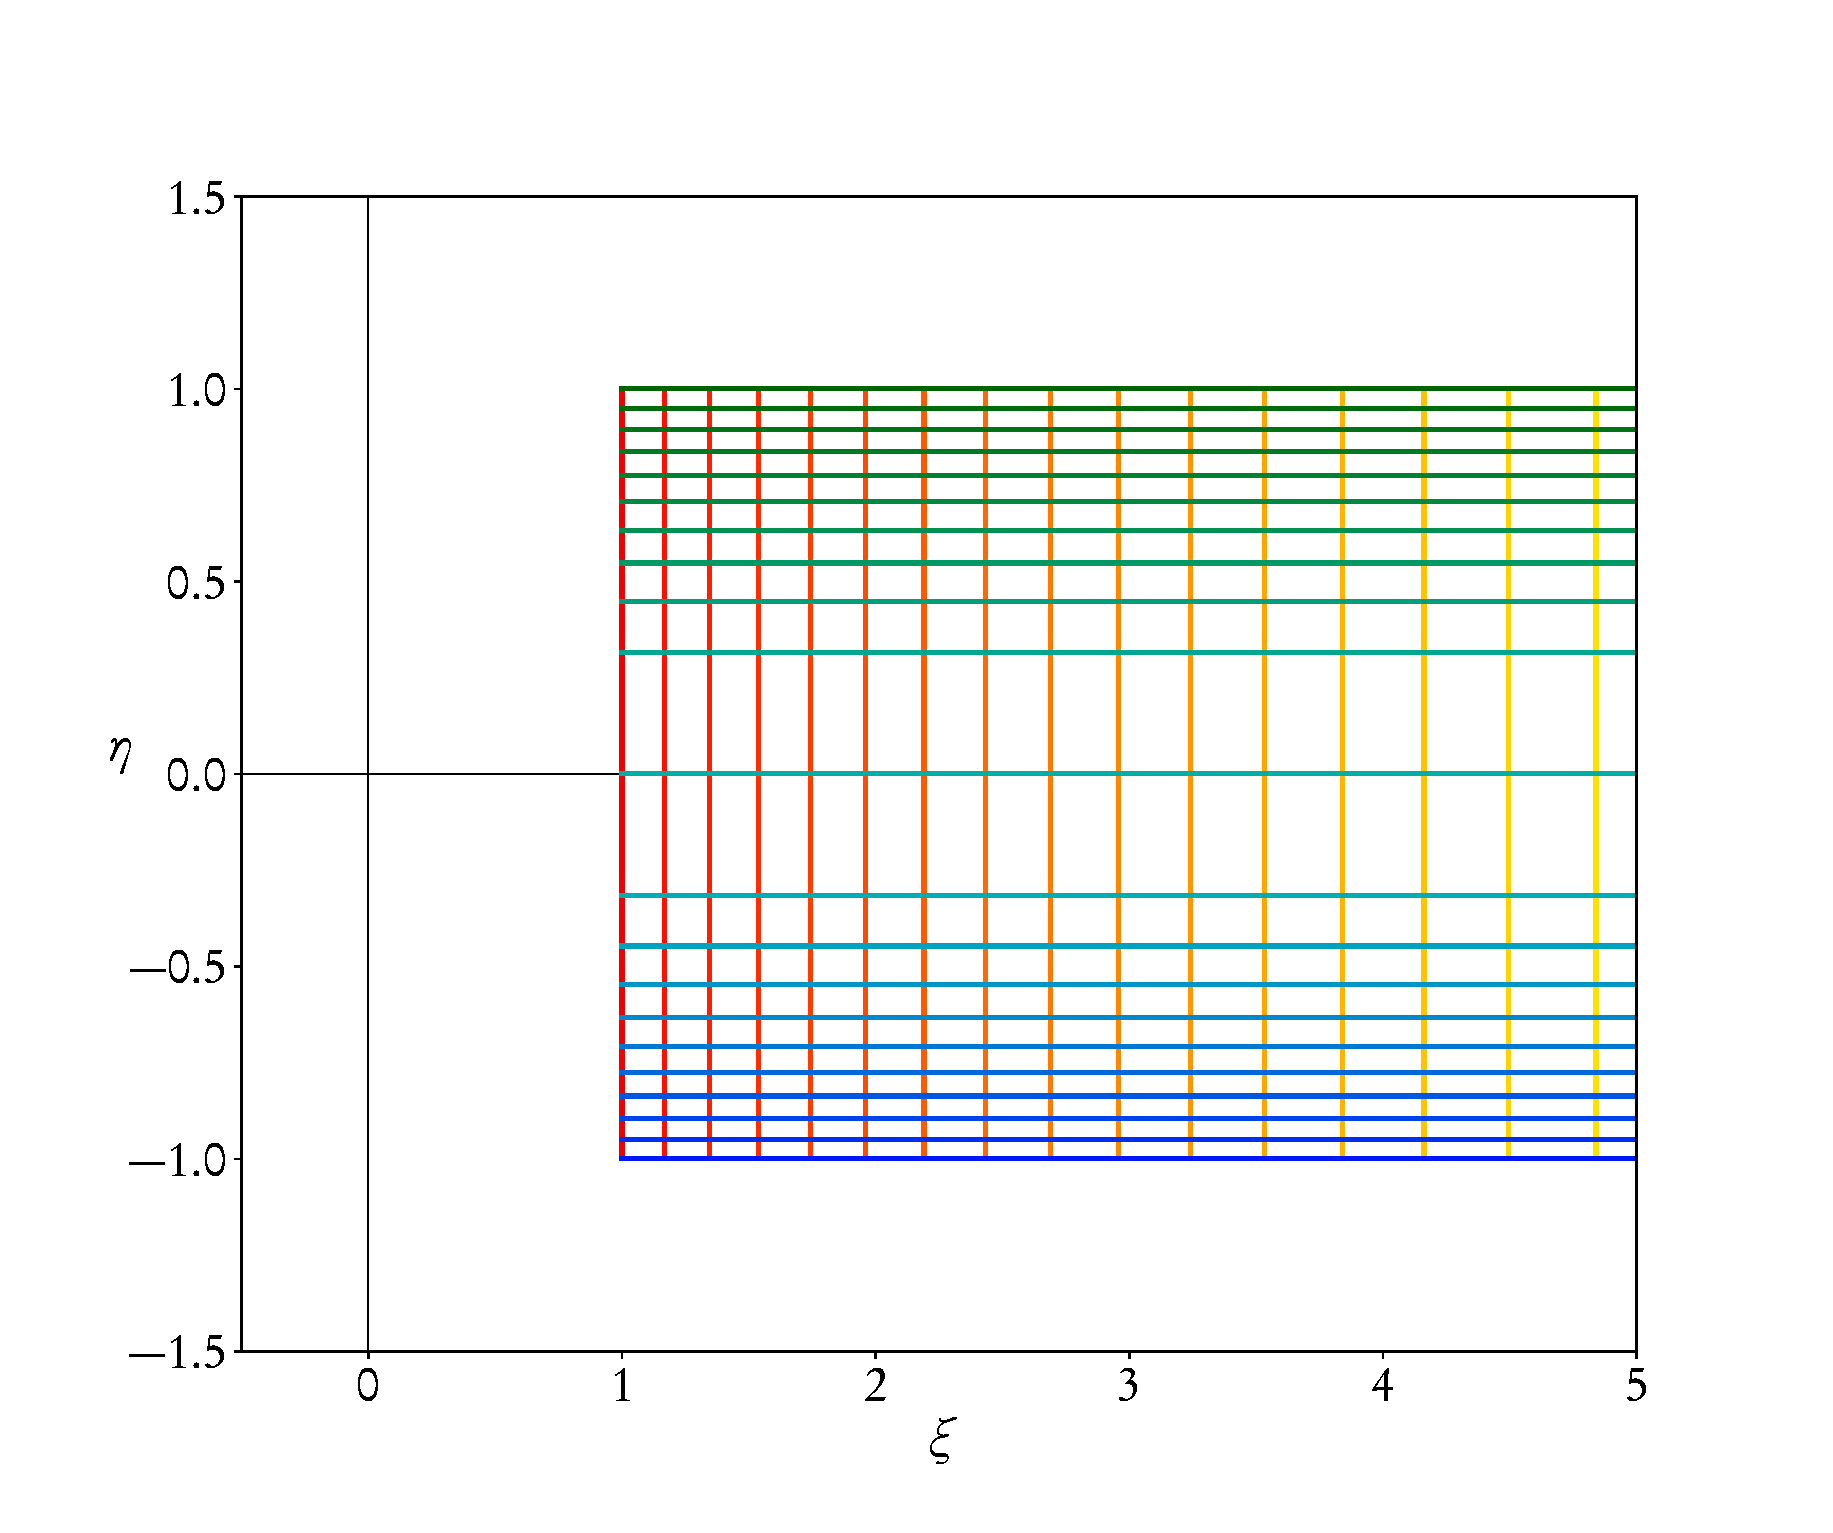
\includegraphics[width=\linewidth]{./images/appendix/xieta.eps}
               \caption{$\xi$-$\eta$ space. \label{fig:xieta}}
            \end{subfigure}%
            \begin{subfigure}{.5\textwidth}
               \centering
               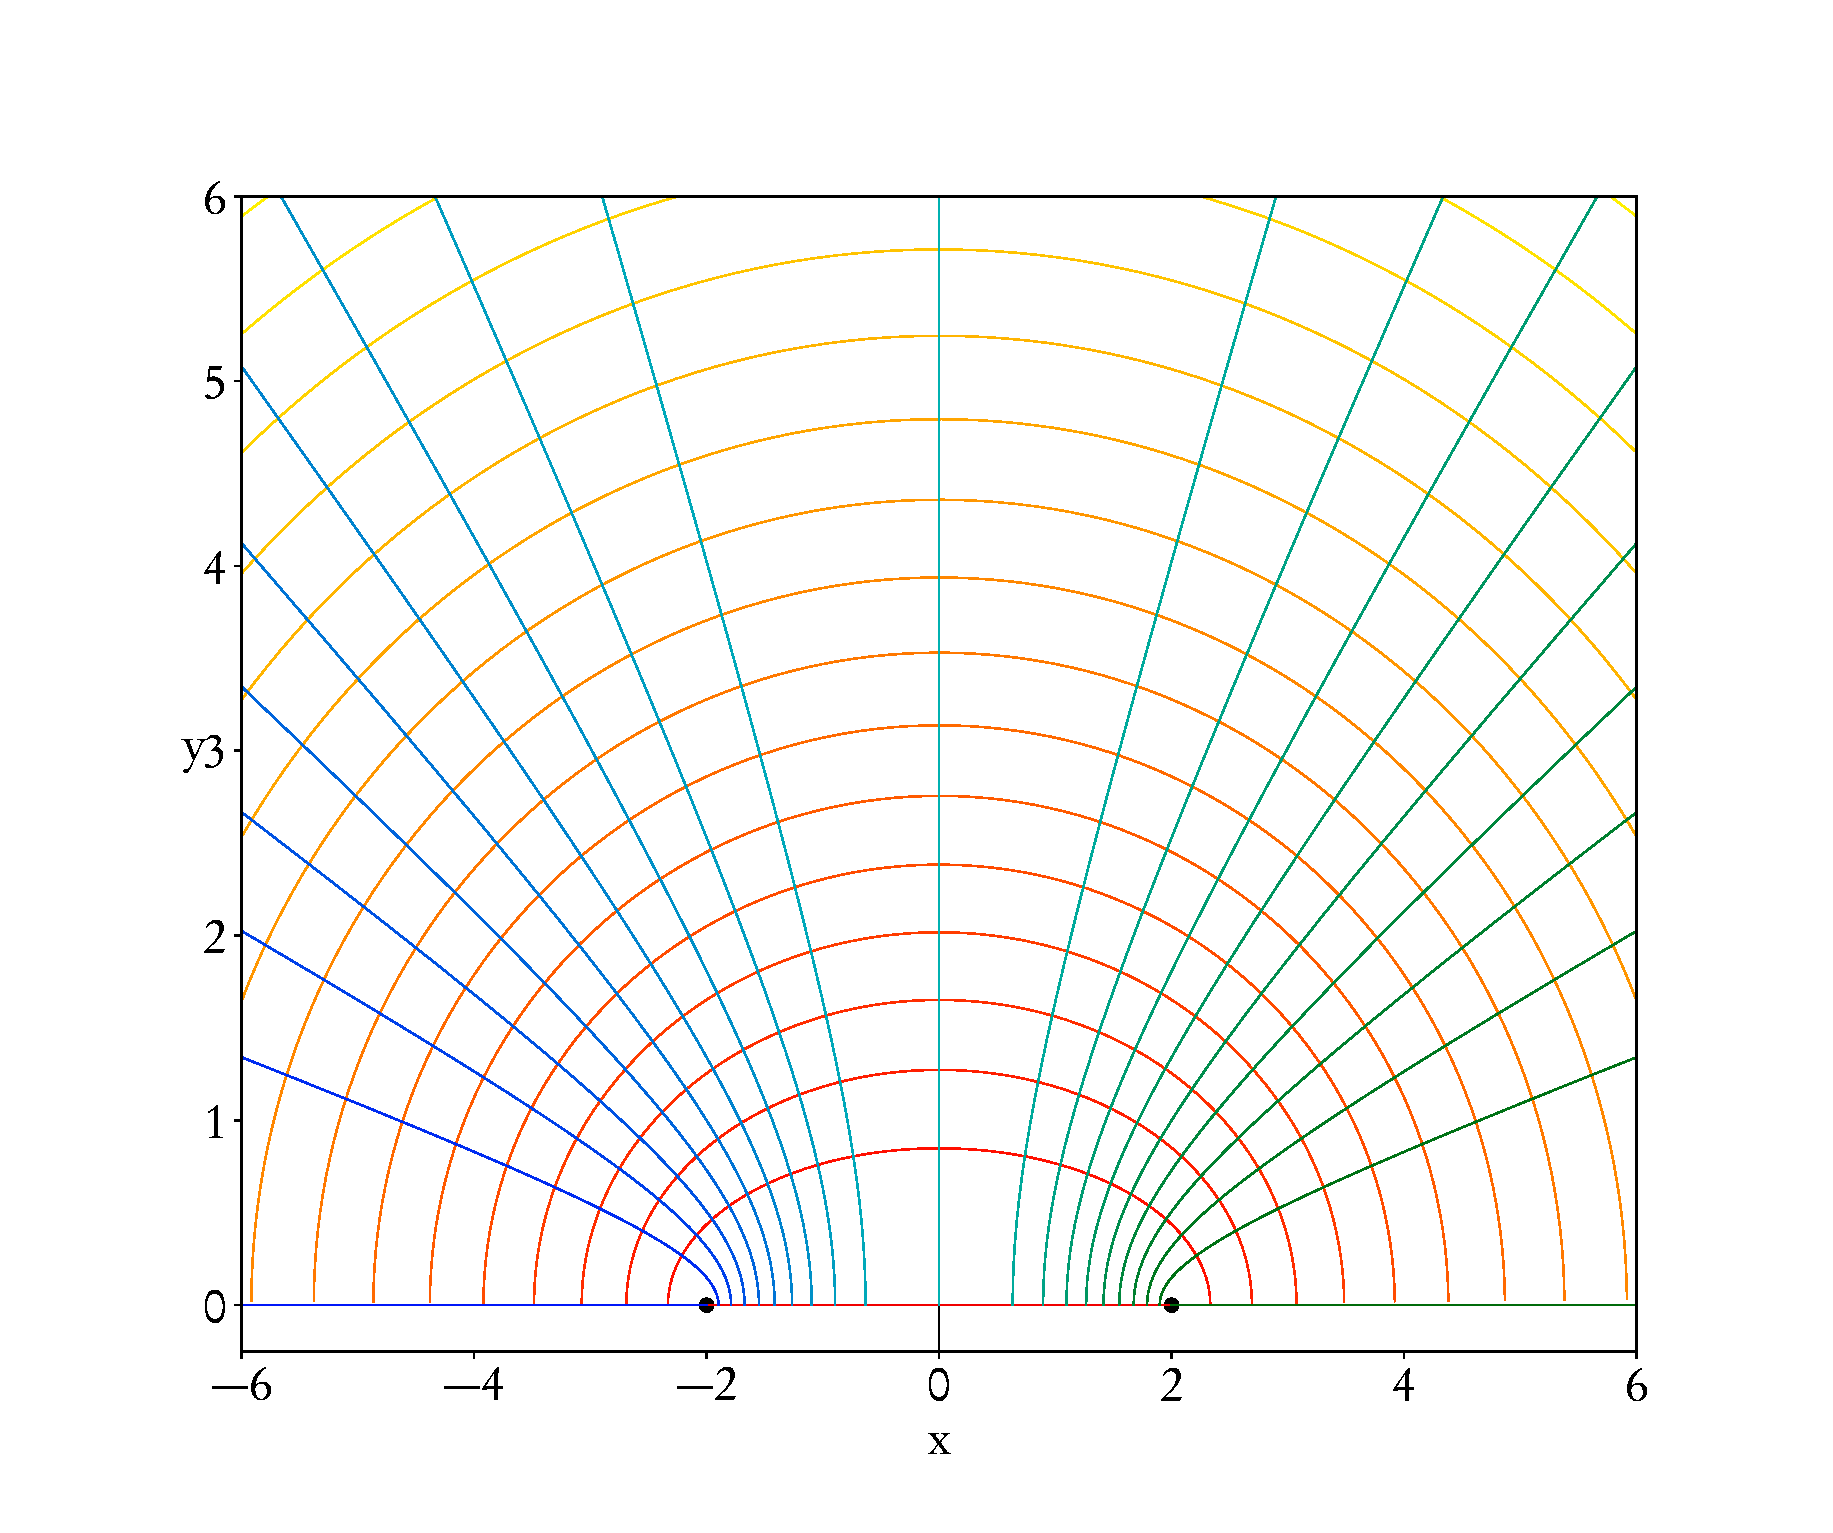
\includegraphics[width=\linewidth]{./images/appendix/eliptical.eps}
               \caption{$x$-$y$ space. \label{fig:xy}}
            \end{subfigure}
            \caption[Coordinate chart of elliptical coordinates]{The coordinate mapping of
                     Eq.~\eqref{eq:elipdef} is demonstrated by the correspondence between
                     coloured grid lines.\label{fig:elliptic}}
         \end{figure}

         Elliptical coordinates are formed by the intersection of series of confocal ellipses and
         hyperbole. If we let $(\xi, \eta)$ denote the elliptic and hyperbolic grid lines and $a > 0$
         their focal length we can cover the plane with two charts. The first is given by
         %
         \begin{equation} \label{eq:elipdef}
            \left\{
            \begin{array}{l}
               x   = a \xi \eta \\
               y^2 = a \left( \xi^2 - 1 \right) \left( 1 - \eta^2 \right),
            \end{array}
            \right.
         \end{equation}
         %
         while the second is defined similarly and covers the lower half space ($(\xi,\eta) \mapsto
         (x,-y)$). Both charts are defined for $(\xi,\eta) \in [1, \infty] \times [-1,1]$ and
         $a = \frac{R}{2}$.

         This mapping is demonstrated in Fig.~\ref{fig:elliptic}. The coloured lines in the left panel
         represent a selection of $\xi$ (blues and greens) and $\eta$ (reds and oranges) grid lines.
         Grid lines are mapped by Eq.~\eqref{eq:elipdef} to lines of corresponding colour in the right
         panel.

      \end{section}

      \begin{section}{Prolate Spheroidal Coordinates \label{sec:prolate}}

         Prolate spheroidal coordinates are a three-dimensional coordinate system that result from
         rotating the upper half space elliptical coordinates (defined in the proceeding section) around
         the line running through the co-foci of the elliptic and hyperbolic grid lines.

         While several conventions exist, throughout this work prolate spheroidal coordinates are
         defined as
         %
         \begin{equation} \label{eq:psc}
            \left\{
            \begin{array}{l}
               x = a \sqrt{(\xi^2 - 1)(1 - \eta^2)} \sin \phi, \\
               y = a \sqrt{(\xi^2 - 1)(1 - \eta^2)} \cos \phi, \\
               z = a \xi \eta,
            \end{array}
            \right.
         \end{equation}
         %
         for $(\xi, \eta, \phi) \in [1, \infty) \times [-1,1] \times [0,2\pi)$.

         One says that a function $f: \mathbb{R}^3 \rightarrow \mathbf{R}$ is cylindrically symmetric if
         it has no $\phi$ dependence, i.e.\ if $f(\xi,\eta,\phi) = f(\xi,\eta)$.

      \end{section}

   \end{chapter}

   \begin{chapter}{The Calculation (bad title) \label{chap:calcdeets}}

      In this appendix details of the code used to calculate the results presented in
      Sec.~\ref{sec:hephe-disc} are presented. This code is an amalgam of several components. These
      consist primarily of the code base developed for carrying out \textsc{tc-bgm} collision
      calculations, here referred to as \texttt{BGM}, the ground-state \textsc{dft} structure code,
      \texttt{DIAMOL}, which can be used to produce a \textsc{ks}-potential for a given arrangement of a
      diatomic molecule, and a short program, \texttt{hephe.py} which manages the execution of a single
      run.

      Both \texttt{BGM} and \texttt{DIAMOL} are mature stand-alone programs. While this makes them well
      suited to preforming their intended function it also makes them somewhat less adaptable. With this
      in mind the design philosophy behind the development of a hybrid code proceeded from a desire to
      modify the existing code as little as possible. Essentially the only modifications made to the
      \texttt{DIAMOL} were to replace a subroutine which calculates the \textsc{ks}-orbitals with one
      which reads the orbitals from a file output by \texttt{BGM}. Similarly the \texttt{BGm} was
      altered to output orbitals to be fed into \texttt{DIAMOL} and to read in potentials output by
      \texttt{DIAMOL}. Additionally execution control was added to \texttt{BGM} which causes it to pause
      and wait for a signal to proceed at each time step, this allows time for a new potential to be
      calculate as necessary.

      These pieces are monitored and controlled by \texttt{hephe.py}. This script servers several
      purposes. First, it sets up the input files needed by \texttt{BGM} and launches two child threads.
      Each thread contains an instance of \texttt{BGM}, one for the spin-up electrons and another for
      spin-down. As These run \texttt{hephe.py} monitors their outputs for a flag which denotes that
      they are ready to receive a new potential. At this point the \texttt{BGM} instances are paused
      and input files needed for \texttt{DIAMOL} are generated from their outputs. Once \texttt{DIAMOL}
      has completed its execution the \texttt{BGM} threads are resumed. In this way the
      \textsc{ks}-orbitals are propagated in a time-dependent potential.

   \end{chapter}

   \begin{chapter}{Three-Electron Correlation Integrals \label{chap:moreIc}}

      The process of deriving three-electron versions of the equations presented in
      Sec.~\ref{sec:phe2p-obs} begins as it did in the two electron state with the full $N$-body wave
      function. Unlike in the former case the wave function is not readily split into spatial and spin
      components. On is then forced to work with the function $\Psi(\mathbf{r}_1, \sigma_1, \mathbf{r}_2,
      \sigma_2, \mathbf{r}_3, \sigma_3, t)$. Our notation may be simplified by introducing a combined
      spatial-spin coordinates $\mathbf{x}_j = (\mathbf{r}_j, \sigma_j)$ and a combined integral
      operator
      %
      \begin{equation} \label{eq:combInt}
         \fint_V \mathrm{d}^3x = \sum\limits_{\sigma = \uparrow, \downarrow} \int_V \mathrm{d}^3 r.
      \end{equation}


      With a slight modification to the definition of the one-particle density
      %
      \begin{equation} \label{eq:xDen}
         n(\mathbf{x}) = N \fint \mathrm{d}^3 x_2 \dots \mathrm{d}^3 x_N
            \left| \Psi( \mathbf{x}, \mathbf{x}_2, \dots, \mathbf{x}_N, t) \right|^2
      \end{equation}
      %
      the single-particle probabilities to find an electron on the target or the projectile may be
      obtained
      %
      \begin{equation}
         p_T = \frac{1}{3} \fint_T n(\mathbf{x},t_f) \, \mathrm{d}^3 x
      \end{equation}
      %
      and
      %
      \begin{equation}
         p_P = \frac{1}{3} \fint_P n(\mathbf{x},t_f) \, \mathrm{d}^3 x.
      \end{equation}
      %
      In addition to these probabilities we will define two varieties of correlation integral, one that
      involves three-particle interactions
      %
      \begin{equation}
         I_\mathrm{c}^{V_1 V_2 V_3} = \fint_{V_1} \fint_{V_2} \fint_{V_3}
           \mathrm{d}^3 x_1 \mathrm{d}^3 x_2 \mathrm{d}^3 x_3 \,
           g^{(3)}_\mathrm{c}(\mathbf{x}_1, \mathbf{x}_2, \mathbf{x}_3, t)
           n(\mathbf{x}_1,t) n(\mathbf{x}_2,t) n(\mathbf{x}_3,t),
      \end{equation}
      %
      \begin{equation}
         g^{(3)}_\mathrm{c}(\mathbf{x}_1, \mathbf{x}_2, \mathbf{x}_3, t) =
            \frac{\rho(\mathbf{x}_1, \mathbf{x}_2, \mathbf{x}_3, t)}
            {n(\mathbf{x}_1,t) n(\mathbf{x}_2,t) n(\mathbf{x}_3,t)} - \frac{1}{9}
      \end{equation}
      %
      and a more familiar two-particle version
      %
      \begin{equation}
         I_\mathrm{c}^{V_1 V_2} = \fint_{V_1} \fint_{V_2} \mathrm{d}^3 x_1 \mathrm{d}^3 x_2 \,
         g^{(2)}_\mathrm{c}(\mathbf{x}_1, \mathbf{x}_2, t) n(\mathbf{x}_1,t) n(\mathbf{x}_2,t),
      \end{equation}
      %
      \begin{equation}
         g^{(2)}_\mathrm{c}(\mathbf{x}_1, \mathbf{x}_2, t) =
         \frac{\rho_2(\mathbf{x}_1, \mathbf{x}_2, t)}
         {n(\mathbf{x}_1,t) n(\mathbf{x}_2,t) } - \frac{1}{3}
      \end{equation}
      %
      where $V_1$, $V_2$, and $V_3 \in \{T,P,I\}$, $\rho = 3|\psi|^2$, and $\rho_2 =
      \fint \mathrm{d}^3 x \rho$.

      With these definitions established the ten outcome probabilities, $p_{kl}$, detailed in
      Sec.~\ref{sec:hephe-det}
      %
      \begin{subequations}
         \begin{equation}
            p_{00} = \frac{1}{3} \fint_T \fint_T \fint_T \rho(\mathbf{x}_1, \mathbf{x}_2,
            \mathbf{x}_3, t_f) \, \mathrm{d}^3 x_1 \mathrm{d}^3 x_2 \mathrm{d}^3 x_3,
         \end{equation}
         %
         \begin{equation}
            p_{01} = \fint_T \fint_T \fint_I \rho(\mathbf{x}_1, \mathbf{x}_2, \mathbf{x}_3, t_f) \,
            \mathrm{d}^3 x_1 \mathrm{d}^3 x_2 \mathrm{d}^3 x_3,
         \end{equation}
         %
         \begin{equation}
            p_{02} = \fint_T \fint_I \fint_I \rho(\mathbf{x}_1, \mathbf{x}_2, \mathbf{x}_3, t_f) \,
            \mathrm{d}^3 x_1 \mathrm{d}^3 x_2 \mathrm{d}^3 x_3,
         \end{equation}
         %
         \begin{equation}
            p_{03} = \frac{1}{3} \fint_I \fint_I \fint_I \rho(\mathbf{x}_1, \mathbf{x}_2,
            \mathbf{x}_3, t_f) \, \mathrm{d}^3 x_1 \mathrm{d}^3 x_2 \mathrm{d}^3 x_3,
         \end{equation}
         %
         \begin{equation}
            p_{10} = \fint_T \fint_T \fint_P \rho(\mathbf{x}_1, \mathbf{x}_2, \mathbf{x}_3, t_f) \,
            \mathrm{d}^3 x_1 \mathrm{d}^3 x_2 \mathrm{d}^3 x_3,
         \end{equation}
         %
         \begin{equation}
            p_{11} = 2 \fint_T \fint_P \fint_I \rho(\mathbf{x}_1, \mathbf{x}_2, \mathbf{x}_3, t_f) \,
            \mathrm{d}^3 x_1 \mathrm{d}^3 x_2 \mathrm{d}^3 x_3,
         \end{equation}
         %
         \begin{equation}
            p_{12} = \fint_P \fint_I \fint_I \rho(\mathbf{x}_1, \mathbf{x}_2, \mathbf{x}_3, t_f) \,
            \mathrm{d}^3 x_1 \mathrm{d}^3 x_2 \mathrm{d}^3 x_3,
         \end{equation}
         %
         \begin{equation}
            p_{20} = \fint_T \fint_P \fint_P \rho(\mathbf{x}_1, \mathbf{x}_2, \mathbf{x}_3, t_f) \,
            \mathrm{d}^3 x_1 \mathrm{d}^3 x_2 \mathrm{d}^3 x_3,
         \end{equation}
         %
         \begin{equation}
            p_{21} = \fint_P \fint_P \fint_I \rho(\mathbf{x}_1, \mathbf{x}_2, \mathbf{x}_3, t_f) \,
            \mathrm{d}^3 x_1 \mathrm{d}^3 x_2 \mathrm{d}^3 x_3,
         \end{equation}
         %
         \begin{equation}
            p_{30} = \frac{1}{3} \fint_P \fint_P \fint_P \rho(\mathbf{x}_1, \mathbf{x}_2,
            \mathbf{x}_3, t_f) \, \mathrm{d}^3 x_1 \mathrm{d}^3 x_2 \mathrm{d}^3 x_3,
         \end{equation}
      \end{subequations}
      %
      may be rewritten as
      %
      \begin{subequations}
         \begin{equation}
            p_{00} = {p_T}^3 + \frac{1}{3} I_\mathrm{c}^{TTT},
         \end{equation}
         %
         \begin{equation}
            p_{01} = 3 {p_T}^2 (1- p_T -p_P) + I_\mathrm{c}^{TT} - I_\mathrm{c}^{TTT}
                   - I_\mathrm{c}^{TTP},
         \end{equation}
         \begin{equation}
            p_{02} = 3 p_T (1 - p_T - p_P)^2 - 2 I_\mathrm{c}^{TT} - 2 I_\mathrm{c}^{TP}
                   + I_\mathrm{c}^{TTT} + 2 I_\mathrm{c}^{TTP} + I_\mathrm{c}^{TPP},
         \end{equation}
         %
         \begin{equation}
            p_{03} = (1 - p_T - p_P)^3 + I_\mathrm{c}^{TT} + 3 I_\mathrm{c}^{TP} + I_\mathrm{c}^{PP}
                   - \frac{1}{3} I_\mathrm{c}^{TTT} - I_\mathrm{c}^{TTP} - I_\mathrm{c}^{TPP}
                   - \frac{1}{3} I_\mathrm{c}^{PPP},
         \end{equation}
         %
         \begin{equation}
            p_{10} = 3{p_T}^2 p_P + I_\mathrm{c}^{TTP},
         \end{equation}
         %
         \begin{equation}
            p_{11} = 6 p_T p_P (1 - p_T - p_P) + 2 I_\mathrm{c}^{TP} - 2 I_\mathrm{c}^{TTP}
                   - 2 I_\mathrm{c}^{TPP},
         \end{equation}
         %
         \begin{equation}
            p_{12} = 3 p_P(1 - p_T - p_P)^2 - 2 I_\mathrm{c}^{TP} - 2 I_\mathrm{c}^{PP}
                   + I_\mathrm{c}^{TTP} + 2 I_\mathrm{c}^{TPP} + I_\mathrm{c}^{PPP},
         \end{equation}
         %
         \begin{equation}
            p_{20} = 3 p_T {p_P}^2 + I_\mathrm{c}^{TPP},
         \end{equation}
         %
         \begin{equation}
            p_{21} = 3 {p_P}^2(1 - p_T - p_P) + I_\mathrm{c}^{PP} - I_\mathrm{c}^{TPP}
                   - I_\mathrm{c}^{PPP},
         \end{equation}
         %
         \begin{equation}
            p_{30} = {p_P}^3 + \frac{1}{3} I_\mathrm{c}^{PPP}.
         \end{equation}
      \end{subequations}

      Just like in the two electron case the \textsc{iem} model may be recovered by setting all
      correlation integrals to zero. One finds
      %
      \begin{subequations} \label{eq:iem3}
         \begin{equation}
            p^\textsc{iem}_{00} = {p_T}^3,
         \end{equation}
         %
         \begin{equation}
            p^\textsc{iem}_{01} = 3 {p_T}^2 (1- p_T -p_P),
         \end{equation}
         %
         \begin{equation}
            p^\textsc{iem}_{02} = 3 p_T (1 - p_T - p_P)^2,
         \end{equation}
         %
         \begin{equation}
            p^\textsc{iem}_{03} = (1 - p_T - p_P)^3,
         \end{equation}
         %
         \begin{equation}
            p^\textsc{iem}_{10} = 3{p_T}^2 p_P,
         \end{equation}
         %
         \begin{equation}
            p^\textsc{iem}_{11} = 6 p_T p_P (1 - p_T - p_P),
         \end{equation}
         %
         \begin{equation}
            p^\textsc{iem}_{12} = 3 p_P(1 - p_T - p_P)^2,
         \end{equation}
         %
         \begin{equation}
            p^\textsc{iem}_{20} = 3 p_T {p_P}^2,
         \end{equation}
         %
         \begin{equation}
            p^\textsc{iem}_{21} = 3 {p_P}^2(1 - p_T - p_P),
         \end{equation}
         %
         \begin{equation}
            p^\textsc{iem}_{30} = {p_P}^3.
         \end{equation}
      \end{subequations}
      %
      Moving beyond an \textsc{iem} description may prove difficult. The failings of the \textsc{wb}
      model, discussed in Chap.~\ref{chap:p-he2p-he}, essentially preclude its application in this more
      complex setting. Any new model envisioned may be aided in part by realtions between the full
      three-particle density and its various reductions (see for example Ref.~\cite{reduce}).

   \end{chapter}

\end{appendices}

\cleardoublepage
\phantomsection
\addcontentsline{toc}{chapter}{References}

\singlespacing

\printbibliography[title=References]

\end{document}

